%
% approx.tex -- daubechies wavelet 2
%
% (c) 2019 Prof Dr Andreas Müller, Hochschule Rapperswil
%
\documentclass[tikz]{standalone}
\usepackage{amsmath}
\usepackage{times}
\usepackage{txfonts}
\usepackage{pgfplots}
\usepackage{csvsimple}
\usetikzlibrary{arrows,intersections,math}
\begin{document}
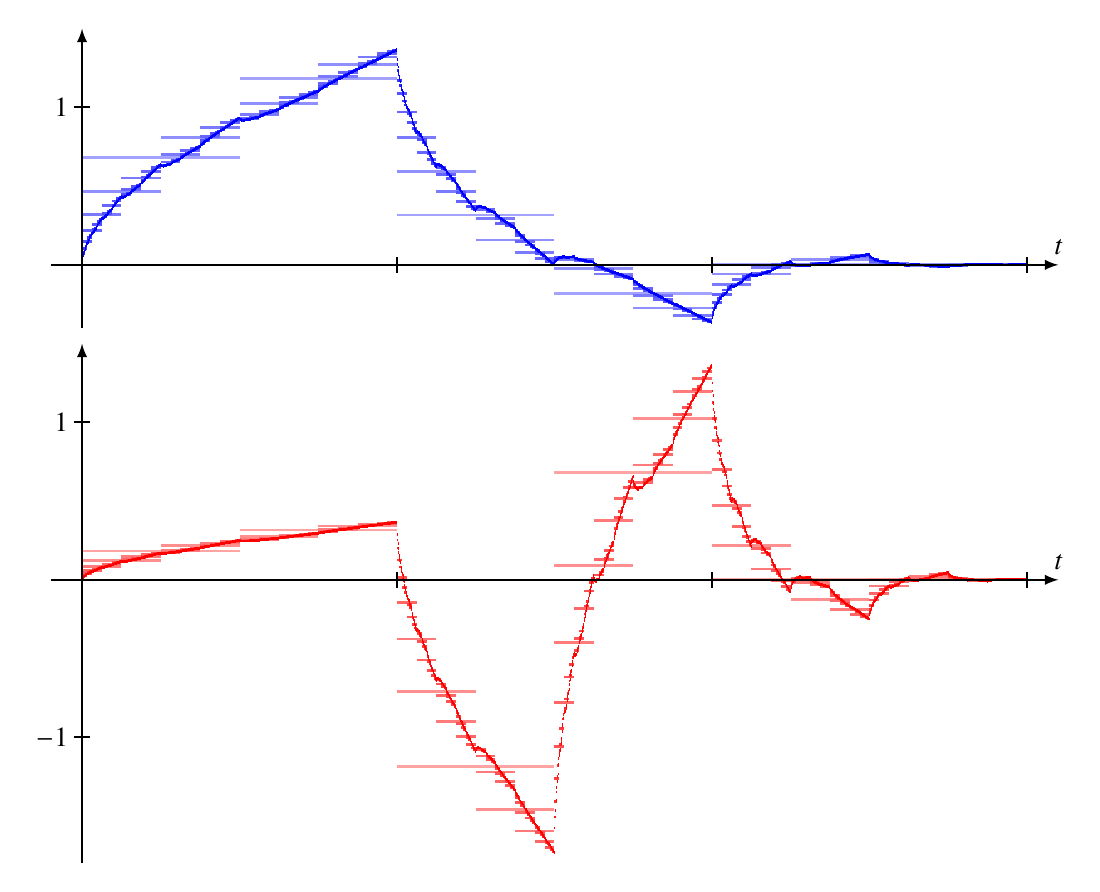
\begin{tikzpicture}[>=latex,yscale=2,xscale=4]

% db1 with J=1
\draw[line width=1pt,color=blue!36] (0.00000,0.68301)--(0.50000,0.68301);
\draw[line width=1pt,color=blue!36] (0.50000,1.18301)--(1.00000,1.18301);
\draw[line width=1pt,color=blue!36] (1.00000,0.31699)--(1.50000,0.31699);
\draw[line width=1pt,color=blue!36] (1.50000,-0.18301)--(2.00000,-0.18301);
\draw[line width=1pt,color=blue!36] (2.00000,0.00000)--(2.50000,0.00000);
\draw[line width=1pt,color=blue!36] (2.50000,0.00000)--(3.00000,0.00000);
% db1 with J=2
\draw[line width=1pt,color=blue!44] (0.00000,0.46651)--(0.25000,0.46651);
\draw[line width=1pt,color=blue!44] (0.25000,0.80801)--(0.50000,0.80801);
\draw[line width=1pt,color=blue!44] (0.50000,1.02452)--(0.75000,1.02452);
\draw[line width=1pt,color=blue!44] (0.75000,1.27452)--(1.00000,1.27452);
\draw[line width=1pt,color=blue!44] (1.00000,0.59151)--(1.25000,0.59151);
\draw[line width=1pt,color=blue!44] (1.25000,0.15849)--(1.50000,0.15849);
\draw[line width=1pt,color=blue!44] (1.50000,-0.02452)--(1.75000,-0.02452);
\draw[line width=1pt,color=blue!44] (1.75000,-0.27452)--(2.00000,-0.27452);
\draw[line width=1pt,color=blue!44] (2.00000,-0.05801)--(2.25000,-0.05801);
\draw[line width=1pt,color=blue!44] (2.25000,0.03349)--(2.50000,0.03349);
\draw[line width=1pt,color=blue!44] (2.50000,0.00000)--(2.75000,0.00000);
\draw[line width=1pt,color=blue!44] (2.75000,0.00000)--(3.00000,0.00000);
% db1 with J=3
\draw[line width=1pt,color=blue!52] (0.00000,0.31863)--(0.12500,0.31863);
\draw[line width=1pt,color=blue!52] (0.12500,0.55188)--(0.25000,0.55188);
\draw[line width=1pt,color=blue!52] (0.25000,0.69976)--(0.37500,0.69976);
\draw[line width=1pt,color=blue!52] (0.37500,0.87051)--(0.50000,0.87051);
\draw[line width=1pt,color=blue!52] (0.50000,0.95589)--(0.62500,0.95589);
\draw[line width=1pt,color=blue!52] (0.62500,1.06414)--(0.75000,1.06414);
\draw[line width=1pt,color=blue!52] (0.75000,1.19527)--(0.87500,1.19527);
\draw[line width=1pt,color=blue!52] (0.87500,1.32027)--(1.00000,1.32027);
\draw[line width=1pt,color=blue!52] (1.00000,0.80801)--(1.12500,0.80801);
\draw[line width=1pt,color=blue!52] (1.12500,0.46651)--(1.25000,0.46651);
\draw[line width=1pt,color=blue!52] (1.25000,0.29575)--(1.37500,0.29575);
\draw[line width=1pt,color=blue!52] (1.37500,0.07925)--(1.50000,0.07925);
\draw[line width=1pt,color=blue!52] (1.50000,0.03349)--(1.62500,0.03349);
\draw[line width=1pt,color=blue!52] (1.62500,-0.05801)--(1.75000,-0.05801);
\draw[line width=1pt,color=blue!52] (1.75000,-0.19527)--(1.87500,-0.19527);
\draw[line width=1pt,color=blue!52] (1.87500,-0.32027)--(2.00000,-0.32027);
\draw[line width=1pt,color=blue!52] (2.00000,-0.12664)--(2.12500,-0.12664);
\draw[line width=1pt,color=blue!52] (2.12500,-0.01839)--(2.25000,-0.01839);
\draw[line width=1pt,color=blue!52] (2.25000,0.00449)--(2.37500,0.00449);
\draw[line width=1pt,color=blue!52] (2.37500,0.05024)--(2.50000,0.05024);
\draw[line width=1pt,color=blue!52] (2.50000,0.01062)--(2.62500,0.01062);
\draw[line width=1pt,color=blue!52] (2.62500,-0.00613)--(2.75000,-0.00613);
\draw[line width=1pt,color=blue!52] (2.75000,0.00000)--(2.87500,0.00000);
\draw[line width=1pt,color=blue!52] (2.87500,0.00000)--(3.00000,0.00000);
% db1 with J=4
\draw[line width=1pt,color=blue!60] (0.00000,0.21763)--(0.06250,0.21763);
\draw[line width=1pt,color=blue!60] (0.06250,0.37694)--(0.12500,0.37694);
\draw[line width=1pt,color=blue!60] (0.12500,0.47794)--(0.18750,0.47794);
\draw[line width=1pt,color=blue!60] (0.18750,0.59457)--(0.25000,0.59457);
\draw[line width=1pt,color=blue!60] (0.25000,0.65288)--(0.31250,0.65288);
\draw[line width=1pt,color=blue!60] (0.31250,0.72682)--(0.37500,0.72682);
\draw[line width=1pt,color=blue!60] (0.37500,0.81639)--(0.43750,0.81639);
\draw[line width=1pt,color=blue!60] (0.43750,0.90176)--(0.50000,0.90176);
\draw[line width=1pt,color=blue!60] (0.50000,0.92883)--(0.56250,0.92883);
\draw[line width=1pt,color=blue!60] (0.56250,0.97151)--(0.62500,0.97151);
\draw[line width=1pt,color=blue!60] (0.62500,1.02983)--(0.68750,1.02983);
\draw[line width=1pt,color=blue!60] (0.68750,1.08395)--(0.75000,1.08395);
\draw[line width=1pt,color=blue!60] (0.75000,1.15371)--(0.81250,1.15371);
\draw[line width=1pt,color=blue!60] (0.81250,1.21927)--(0.87500,1.21927);
\draw[line width=1pt,color=blue!60] (0.87500,1.28065)--(0.93750,1.28065);
\draw[line width=1pt,color=blue!60] (0.93750,1.34315)--(1.00000,1.34315);
\draw[line width=1pt,color=blue!60] (1.00000,0.97039)--(1.06250,0.97039);
\draw[line width=1pt,color=blue!60] (1.06250,0.71426)--(1.12500,0.71426);
\draw[line width=1pt,color=blue!60] (1.12500,0.57476)--(1.18750,0.57476);
\draw[line width=1pt,color=blue!60] (1.18750,0.40401)--(1.25000,0.40401);
\draw[line width=1pt,color=blue!60] (1.25000,0.34988)--(1.31250,0.34988);
\draw[line width=1pt,color=blue!60] (1.31250,0.26450)--(1.37500,0.26450);
\draw[line width=1pt,color=blue!60] (1.37500,0.14788)--(1.43750,0.14788);
\draw[line width=1pt,color=blue!60] (1.43750,0.03962)--(1.50000,0.03962);
\draw[line width=1pt,color=blue!60] (1.50000,0.04800)--(1.56250,0.04800);
\draw[line width=1pt,color=blue!60] (1.56250,0.02512)--(1.62500,0.02512);
\draw[line width=1pt,color=blue!60] (1.62500,-0.02901)--(1.68750,-0.02901);
\draw[line width=1pt,color=blue!60] (1.68750,-0.07476)--(1.75000,-0.07476);
\draw[line width=1pt,color=blue!60] (1.75000,-0.15176)--(1.81250,-0.15176);
\draw[line width=1pt,color=blue!60] (1.81250,-0.22039)--(1.87500,-0.22039);
\draw[line width=1pt,color=blue!60] (1.87500,-0.28065)--(1.93750,-0.28065);
\draw[line width=1pt,color=blue!60] (1.93750,-0.34315)--(2.00000,-0.34315);
\draw[line width=1pt,color=blue!60] (2.00000,-0.18802)--(2.06250,-0.18802);
\draw[line width=1pt,color=blue!60] (2.06250,-0.09121)--(2.12500,-0.09121);
\draw[line width=1pt,color=blue!60] (2.12500,-0.05270)--(2.18750,-0.05270);
\draw[line width=1pt,color=blue!60] (2.18750,0.00142)--(2.25000,0.00142);
\draw[line width=1pt,color=blue!60] (2.25000,-0.00276)--(2.31250,-0.00276);
\draw[line width=1pt,color=blue!60] (2.31250,0.00867)--(2.37500,0.00867);
\draw[line width=1pt,color=blue!60] (2.37500,0.03574)--(2.43750,0.03574);
\draw[line width=1pt,color=blue!60] (2.43750,0.05861)--(2.50000,0.05861);
\draw[line width=1pt,color=blue!60] (2.50000,0.02318)--(2.56250,0.02318);
\draw[line width=1pt,color=blue!60] (2.56250,0.00337)--(2.62500,0.00337);
\draw[line width=1pt,color=blue!60] (2.62500,-0.00082)--(2.68750,-0.00082);
\draw[line width=1pt,color=blue!60] (2.68750,-0.00919)--(2.75000,-0.00919);
\draw[line width=1pt,color=blue!60] (2.75000,-0.00194)--(2.81250,-0.00194);
\draw[line width=1pt,color=blue!60] (2.81250,0.00112)--(2.87500,0.00112);
\draw[line width=1pt,color=blue!60] (2.87500,0.00000)--(2.93750,0.00000);
\draw[line width=1pt,color=blue!60] (2.93750,0.00000)--(3.00000,0.00000);
% db1 with J=5
\draw[line width=1pt,color=blue!68] (0.00000,0.14864)--(0.03125,0.14864);
\draw[line width=1pt,color=blue!68] (0.03125,0.25746)--(0.06250,0.25746);
\draw[line width=1pt,color=blue!68] (0.06250,0.32644)--(0.09375,0.32644);
\draw[line width=1pt,color=blue!68] (0.09375,0.40610)--(0.12500,0.40610);
\draw[line width=1pt,color=blue!68] (0.12500,0.44593)--(0.15625,0.44593);
\draw[line width=1pt,color=blue!68] (0.15625,0.49643)--(0.18750,0.49643);
\draw[line width=1pt,color=blue!68] (0.18750,0.55760)--(0.21875,0.55760);
\draw[line width=1pt,color=blue!68] (0.21875,0.61592)--(0.25000,0.61592);
\draw[line width=1pt,color=blue!68] (0.25000,0.63440)--(0.28125,0.63440);
\draw[line width=1pt,color=blue!68] (0.28125,0.66356)--(0.31250,0.66356);
\draw[line width=1pt,color=blue!68] (0.31250,0.70339)--(0.34375,0.70339);
\draw[line width=1pt,color=blue!68] (0.34375,0.74035)--(0.37500,0.74035);
\draw[line width=1pt,color=blue!68] (0.37500,0.78800)--(0.40625,0.78800);
\draw[line width=1pt,color=blue!68] (0.40625,0.83278)--(0.43750,0.83278);
\draw[line width=1pt,color=blue!68] (0.43750,0.87470)--(0.46875,0.87470);
\draw[line width=1pt,color=blue!68] (0.46875,0.91739)--(0.50000,0.91739);
\draw[line width=1pt,color=blue!68] (0.50000,0.92025)--(0.53125,0.92025);
\draw[line width=1pt,color=blue!68] (0.53125,0.93378)--(0.56250,0.93378);
\draw[line width=1pt,color=blue!68] (0.56250,0.95798)--(0.59375,0.95798);
\draw[line width=1pt,color=blue!68] (0.59375,0.97933)--(0.62500,0.97933);
\draw[line width=1pt,color=blue!68] (0.62500,1.01134)--(0.65625,1.01134);
\draw[line width=1pt,color=blue!68] (0.65625,1.04050)--(0.68750,1.04050);
\draw[line width=1pt,color=blue!68] (0.68750,1.06680)--(0.71875,1.06680);
\draw[line width=1pt,color=blue!68] (0.71875,1.09386)--(0.75000,1.09386);
\draw[line width=1pt,color=blue!68] (0.75000,1.13160)--(0.78125,1.13160);
\draw[line width=1pt,color=blue!68] (0.78125,1.16647)--(0.81250,1.16647);
\draw[line width=1pt,color=blue!68] (0.81250,1.19849)--(0.84375,1.19849);
\draw[line width=1pt,color=blue!68] (0.84375,1.23127)--(0.87500,1.23127);
\draw[line width=1pt,color=blue!68] (0.87500,1.26119)--(0.90625,1.26119);
\draw[line width=1pt,color=blue!68] (0.90625,1.29188)--(0.93750,1.29188);
\draw[line width=1pt,color=blue!68] (0.93750,1.32334)--(0.96875,1.32334);
\draw[line width=1pt,color=blue!68] (0.96875,1.35459)--(1.00000,1.35459);
\draw[line width=1pt,color=blue!68] (1.00000,1.08855)--(1.03125,1.08855);
\draw[line width=1pt,color=blue!68] (1.03125,0.90217)--(1.06250,0.90217);
\draw[line width=1pt,color=blue!68] (1.06250,0.79545)--(1.09375,0.79545);
\draw[line width=1pt,color=blue!68] (1.09375,0.66739)--(1.12500,0.66739);
\draw[line width=1pt,color=blue!68] (1.12500,0.61898)--(1.15625,0.61898);
\draw[line width=1pt,color=blue!68] (1.15625,0.54923)--(1.18750,0.54923);
\draw[line width=1pt,color=blue!68] (1.18750,0.45813)--(1.21875,0.45813);
\draw[line width=1pt,color=blue!68] (1.21875,0.37276)--(1.25000,0.37276);
\draw[line width=1pt,color=blue!68] (1.25000,0.36704)--(1.28125,0.36704);
\draw[line width=1pt,color=blue!68] (1.28125,0.33997)--(1.31250,0.33997);
\draw[line width=1pt,color=blue!68] (1.31250,0.29157)--(1.34375,0.29157);
\draw[line width=1pt,color=blue!68] (1.34375,0.24888)--(1.37500,0.24888);
\draw[line width=1pt,color=blue!68] (1.37500,0.18485)--(1.40625,0.18485);
\draw[line width=1pt,color=blue!68] (1.40625,0.12653)--(1.43750,0.12653);
\draw[line width=1pt,color=blue!68] (1.43750,0.07394)--(1.46875,0.07394);
\draw[line width=1pt,color=blue!68] (1.46875,0.01981)--(1.50000,0.01981);
\draw[line width=1pt,color=blue!68] (1.50000,0.04534)--(1.53125,0.04534);
\draw[line width=1pt,color=blue!68] (1.53125,0.04953)--(1.56250,0.04953);
\draw[line width=1pt,color=blue!68] (1.56250,0.03237)--(1.59375,0.03237);
\draw[line width=1pt,color=blue!68] (1.59375,0.02093)--(1.62500,0.02093);
\draw[line width=1pt,color=blue!68] (1.62500,-0.01185)--(1.65625,-0.01185);
\draw[line width=1pt,color=blue!68] (1.65625,-0.03891)--(1.68750,-0.03891);
\draw[line width=1pt,color=blue!68] (1.68750,-0.06026)--(1.71875,-0.06026);
\draw[line width=1pt,color=blue!68] (1.71875,-0.08313)--(1.75000,-0.08313);
\draw[line width=1pt,color=blue!68] (1.75000,-0.12735)--(1.78125,-0.12735);
\draw[line width=1pt,color=blue!68] (1.78125,-0.16586)--(1.81250,-0.16586);
\draw[line width=1pt,color=blue!68] (1.81250,-0.19864)--(1.84375,-0.19864);
\draw[line width=1pt,color=blue!68] (1.84375,-0.23295)--(1.87500,-0.23295);
\draw[line width=1pt,color=blue!68] (1.87500,-0.26155)--(1.90625,-0.26155);
\draw[line width=1pt,color=blue!68] (1.90625,-0.29168)--(1.93750,-0.29168);
\draw[line width=1pt,color=blue!68] (1.93750,-0.32334)--(1.96875,-0.32334);
\draw[line width=1pt,color=blue!68] (1.96875,-0.35459)--(2.00000,-0.35459);
\draw[line width=1pt,color=blue!68] (2.00000,-0.23719)--(2.03125,-0.23719);
\draw[line width=1pt,color=blue!68] (2.03125,-0.15963)--(2.06250,-0.15963);
\draw[line width=1pt,color=blue!68] (2.06250,-0.12189)--(2.09375,-0.12189);
\draw[line width=1pt,color=blue!68] (2.09375,-0.07349)--(2.12500,-0.07349);
\draw[line width=1pt,color=blue!68] (2.12500,-0.06491)--(2.15625,-0.06491);
\draw[line width=1pt,color=blue!68] (2.15625,-0.04566)--(2.18750,-0.04566);
\draw[line width=1pt,color=blue!68] (2.18750,-0.01574)--(2.21875,-0.01574);
\draw[line width=1pt,color=blue!68] (2.21875,0.01133)--(2.25000,0.01133);
\draw[line width=1pt,color=blue!68] (2.25000,-0.00144)--(2.28125,-0.00144);
\draw[line width=1pt,color=blue!68] (2.28125,-0.00353)--(2.31250,-0.00353);
\draw[line width=1pt,color=blue!68] (2.31250,0.00505)--(2.34375,0.00505);
\draw[line width=1pt,color=blue!68] (2.34375,0.01077)--(2.37500,0.01077);
\draw[line width=1pt,color=blue!68] (2.37500,0.02716)--(2.40625,0.02716);
\draw[line width=1pt,color=blue!68] (2.40625,0.04069)--(2.43750,0.04069);
\draw[line width=1pt,color=blue!68] (2.43750,0.05136)--(2.46875,0.05136);
\draw[line width=1pt,color=blue!68] (2.46875,0.06280)--(2.50000,0.06280);
\draw[line width=1pt,color=blue!68] (2.50000,0.03441)--(2.53125,0.03441);
\draw[line width=1pt,color=blue!68] (2.53125,0.01669)--(2.56250,0.01669);
\draw[line width=1pt,color=blue!68] (2.56250,0.00965)--(2.59375,0.00965);
\draw[line width=1pt,color=blue!68] (2.59375,-0.00026)--(2.62500,-0.00026);
\draw[line width=1pt,color=blue!68] (2.62500,0.00051)--(2.65625,0.00051);
\draw[line width=1pt,color=blue!68] (2.65625,-0.00159)--(2.68750,-0.00159);
\draw[line width=1pt,color=blue!68] (2.68750,-0.00654)--(2.71875,-0.00654);
\draw[line width=1pt,color=blue!68] (2.71875,-0.01073)--(2.75000,-0.01073);
\draw[line width=1pt,color=blue!68] (2.75000,-0.00424)--(2.78125,-0.00424);
\draw[line width=1pt,color=blue!68] (2.78125,-0.00062)--(2.81250,-0.00062);
\draw[line width=1pt,color=blue!68] (2.81250,0.00015)--(2.84375,0.00015);
\draw[line width=1pt,color=blue!68] (2.84375,0.00168)--(2.87500,0.00168);
\draw[line width=1pt,color=blue!68] (2.87500,0.00036)--(2.90625,0.00036);
\draw[line width=1pt,color=blue!68] (2.90625,-0.00021)--(2.93750,-0.00021);
\draw[line width=1pt,color=blue!68] (2.93750,0.00000)--(2.96875,0.00000);
\draw[line width=1pt,color=blue!68] (2.96875,0.00000)--(3.00000,0.00000);
% db1 with J=6
\draw[line width=1pt,color=blue!76] (0.00000,0.10152)--(0.01562,0.10152);
\draw[line width=1pt,color=blue!76] (0.01562,0.17585)--(0.03125,0.17585);
\draw[line width=1pt,color=blue!76] (0.03125,0.22296)--(0.04688,0.22296);
\draw[line width=1pt,color=blue!76] (0.04688,0.27737)--(0.06250,0.27737);
\draw[line width=1pt,color=blue!76] (0.06250,0.30457)--(0.07812,0.30457);
\draw[line width=1pt,color=blue!76] (0.07812,0.33907)--(0.09375,0.33907);
\draw[line width=1pt,color=blue!76] (0.09375,0.38085)--(0.10938,0.38085);
\draw[line width=1pt,color=blue!76] (0.10938,0.42068)--(0.12500,0.42068);
\draw[line width=1pt,color=blue!76] (0.12500,0.43330)--(0.14062,0.43330);
\draw[line width=1pt,color=blue!76] (0.14062,0.45322)--(0.15625,0.45322);
\draw[line width=1pt,color=blue!76] (0.15625,0.48042)--(0.17188,0.48042);
\draw[line width=1pt,color=blue!76] (0.17188,0.50567)--(0.18750,0.50567);
\draw[line width=1pt,color=blue!76] (0.18750,0.53821)--(0.20312,0.53821);
\draw[line width=1pt,color=blue!76] (0.20312,0.56880)--(0.21875,0.56880);
\draw[line width=1pt,color=blue!76] (0.21875,0.59743)--(0.23438,0.59743);
\draw[line width=1pt,color=blue!76] (0.23438,0.62659)--(0.25000,0.62659);
\draw[line width=1pt,color=blue!76] (0.25000,0.62854)--(0.26562,0.62854);
\draw[line width=1pt,color=blue!76] (0.26562,0.63778)--(0.28125,0.63778);
\draw[line width=1pt,color=blue!76] (0.28125,0.65431)--(0.29688,0.65431);
\draw[line width=1pt,color=blue!76] (0.29688,0.66889)--(0.31250,0.66889);
\draw[line width=1pt,color=blue!76] (0.31250,0.69076)--(0.32812,0.69076);
\draw[line width=1pt,color=blue!76] (0.32812,0.71067)--(0.34375,0.71067);
\draw[line width=1pt,color=blue!76] (0.34375,0.72864)--(0.35938,0.72864);
\draw[line width=1pt,color=blue!76] (0.35938,0.74712)--(0.37500,0.74712);
\draw[line width=1pt,color=blue!76] (0.37500,0.77289)--(0.39062,0.77289);
\draw[line width=1pt,color=blue!76] (0.39062,0.79671)--(0.40625,0.79671);
\draw[line width=1pt,color=blue!76] (0.40625,0.81858)--(0.42188,0.81858);
\draw[line width=1pt,color=blue!76] (0.42188,0.84097)--(0.43750,0.84097);
\draw[line width=1pt,color=blue!76] (0.43750,0.86141)--(0.45312,0.86141);
\draw[line width=1pt,color=blue!76] (0.45312,0.88237)--(0.46875,0.88237);
\draw[line width=1pt,color=blue!76] (0.46875,0.90386)--(0.48438,0.90386);
\draw[line width=1pt,color=blue!76] (0.48438,0.92520)--(0.50000,0.92520);
\draw[line width=1pt,color=blue!76] (0.50000,0.91934)--(0.51562,0.91934);
\draw[line width=1pt,color=blue!76] (0.51562,0.92077)--(0.53125,0.92077);
\draw[line width=1pt,color=blue!76] (0.53125,0.92949)--(0.54688,0.92949);
\draw[line width=1pt,color=blue!76] (0.54688,0.93626)--(0.56250,0.93626);
\draw[line width=1pt,color=blue!76] (0.56250,0.95031)--(0.57812,0.95031);
\draw[line width=1pt,color=blue!76] (0.57812,0.96241)--(0.59375,0.96241);
\draw[line width=1pt,color=blue!76] (0.59375,0.97256)--(0.60938,0.97256);
\draw[line width=1pt,color=blue!76] (0.60938,0.98323)--(0.62500,0.98323);
\draw[line width=1pt,color=blue!76] (0.62500,1.00119)--(0.64062,1.00119);
\draw[line width=1pt,color=blue!76] (0.64062,1.01720)--(0.65625,1.01720);
\draw[line width=1pt,color=blue!76] (0.65625,1.03126)--(0.67188,1.03126);
\draw[line width=1pt,color=blue!76] (0.67188,1.04584)--(0.68750,1.04584);
\draw[line width=1pt,color=blue!76] (0.68750,1.05846)--(0.70312,1.05846);
\draw[line width=1pt,color=blue!76] (0.70312,1.07161)--(0.71875,1.07161);
\draw[line width=1pt,color=blue!76] (0.71875,1.08528)--(0.73438,1.08528);
\draw[line width=1pt,color=blue!76] (0.73438,1.09881)--(0.75000,1.09881);
\draw[line width=1pt,color=blue!76] (0.75000,1.11963)--(0.76562,1.11963);
\draw[line width=1pt,color=blue!76] (0.76562,1.13850)--(0.78125,1.13850);
\draw[line width=1pt,color=blue!76] (0.78125,1.15542)--(0.79688,1.15542);
\draw[line width=1pt,color=blue!76] (0.79688,1.17285)--(0.81250,1.17285);
\draw[line width=1pt,color=blue!76] (0.81250,1.18834)--(0.82812,1.18834);
\draw[line width=1pt,color=blue!76] (0.82812,1.20435)--(0.84375,1.20435);
\draw[line width=1pt,color=blue!76] (0.84375,1.22088)--(0.85938,1.22088);
\draw[line width=1pt,color=blue!76] (0.85938,1.23727)--(0.87500,1.23727);
\draw[line width=1pt,color=blue!76] (0.87500,1.25171)--(0.89062,1.25171);
\draw[line width=1pt,color=blue!76] (0.89062,1.26667)--(0.90625,1.26667);
\draw[line width=1pt,color=blue!76] (0.90625,1.28215)--(0.92188,1.28215);
\draw[line width=1pt,color=blue!76] (0.92188,1.29750)--(0.93750,1.29750);
\draw[line width=1pt,color=blue!76] (0.93750,1.31337)--(0.95312,1.31337);
\draw[line width=1pt,color=blue!76] (0.95312,1.32909)--(0.96875,1.32909);
\draw[line width=1pt,color=blue!76] (0.96875,1.34468)--(0.98438,1.34468);
\draw[line width=1pt,color=blue!76] (0.98438,1.36031)--(1.00000,1.36031);
\draw[line width=1pt,color=blue!76] (1.00000,1.17288)--(1.01562,1.17288);
\draw[line width=1pt,color=blue!76] (1.01562,1.03986)--(1.03125,1.03986);
\draw[line width=1pt,color=blue!76] (1.03125,0.96125)--(1.04688,0.96125);
\draw[line width=1pt,color=blue!76] (1.04688,0.86806)--(1.06250,0.86806);
\draw[line width=1pt,color=blue!76] (1.06250,0.82928)--(1.07812,0.82928);
\draw[line width=1pt,color=blue!76] (1.07812,0.77592)--(1.09375,0.77592);
\draw[line width=1pt,color=blue!76] (1.09375,0.70798)--(1.10938,0.70798);
\draw[line width=1pt,color=blue!76] (1.10938,0.64395)--(1.12500,0.64395);
\draw[line width=1pt,color=blue!76] (1.12500,0.63432)--(1.14062,0.63432);
\draw[line width=1pt,color=blue!76] (1.14062,0.61012)--(1.15625,0.61012);
\draw[line width=1pt,color=blue!76] (1.15625,0.57134)--(1.17188,0.57134);
\draw[line width=1pt,color=blue!76] (1.17188,0.53646)--(1.18750,0.53646);
\draw[line width=1pt,color=blue!76] (1.18750,0.48701)--(1.20312,0.48701);
\draw[line width=1pt,color=blue!76] (1.20312,0.44146)--(1.21875,0.44146);
\draw[line width=1pt,color=blue!76] (1.21875,0.39982)--(1.23438,0.39982);
\draw[line width=1pt,color=blue!76] (1.23438,0.35713)--(1.25000,0.35713);
\draw[line width=1pt,color=blue!76] (1.25000,0.36885)--(1.26562,0.36885);
\draw[line width=1pt,color=blue!76] (1.26562,0.36599)--(1.28125,0.36599);
\draw[line width=1pt,color=blue!76] (1.28125,0.34855)--(1.29688,0.34855);
\draw[line width=1pt,color=blue!76] (1.29688,0.33502)--(1.31250,0.33502);
\draw[line width=1pt,color=blue!76] (1.31250,0.30691)--(1.32812,0.30691);
\draw[line width=1pt,color=blue!76] (1.32812,0.28271)--(1.34375,0.28271);
\draw[line width=1pt,color=blue!76] (1.34375,0.26241)--(1.35938,0.26241);
\draw[line width=1pt,color=blue!76] (1.35938,0.24107)--(1.37500,0.24107);
\draw[line width=1pt,color=blue!76] (1.37500,0.20514)--(1.39062,0.20514);
\draw[line width=1pt,color=blue!76] (1.39062,0.17313)--(1.40625,0.17313);
\draw[line width=1pt,color=blue!76] (1.40625,0.14502)--(1.42188,0.14502);
\draw[line width=1pt,color=blue!76] (1.42188,0.11586)--(1.43750,0.11586);
\draw[line width=1pt,color=blue!76] (1.43750,0.09061)--(1.45312,0.09061);
\draw[line width=1pt,color=blue!76] (1.45312,0.06431)--(1.46875,0.06431);
\draw[line width=1pt,color=blue!76] (1.46875,0.03697)--(1.48438,0.03697);
\draw[line width=1pt,color=blue!76] (1.48438,0.00991)--(1.50000,0.00991);
\draw[line width=1pt,color=blue!76] (1.50000,0.03725)--(1.51562,0.03725);
\draw[line width=1pt,color=blue!76] (1.51562,0.05002)--(1.53125,0.05002);
\draw[line width=1pt,color=blue!76] (1.53125,0.04820)--(1.54688,0.04820);
\draw[line width=1pt,color=blue!76] (1.54688,0.05030)--(1.56250,0.05030);
\draw[line width=1pt,color=blue!76] (1.56250,0.03781)--(1.57812,0.03781);
\draw[line width=1pt,color=blue!76] (1.57812,0.02923)--(1.59375,0.02923);
\draw[line width=1pt,color=blue!76] (1.59375,0.02456)--(1.60938,0.02456);
\draw[line width=1pt,color=blue!76] (1.60938,0.01884)--(1.62500,0.01884);
\draw[line width=1pt,color=blue!76] (1.62500,-0.00146)--(1.64062,-0.00146);
\draw[line width=1pt,color=blue!76] (1.64062,-0.01785)--(1.65625,-0.01785);
\draw[line width=1pt,color=blue!76] (1.65625,-0.03033)--(1.67188,-0.03033);
\draw[line width=1pt,color=blue!76] (1.67188,-0.04387)--(1.68750,-0.04387);
\draw[line width=1pt,color=blue!76] (1.68750,-0.05349)--(1.70312,-0.05349);
\draw[line width=1pt,color=blue!76] (1.70312,-0.06416)--(1.71875,-0.06416);
\draw[line width=1pt,color=blue!76] (1.71875,-0.07588)--(1.73438,-0.07588);
\draw[line width=1pt,color=blue!76] (1.73438,-0.08732)--(1.75000,-0.08732);
\draw[line width=1pt,color=blue!76] (1.75000,-0.11334)--(1.76562,-0.11334);
\draw[line width=1pt,color=blue!76] (1.76562,-0.13545)--(1.78125,-0.13545);
\draw[line width=1pt,color=blue!76] (1.78125,-0.15365)--(1.79688,-0.15365);
\draw[line width=1pt,color=blue!76] (1.79688,-0.17290)--(1.81250,-0.17290);
\draw[line width=1pt,color=blue!76] (1.81250,-0.18825)--(1.82812,-0.18825);
\draw[line width=1pt,color=blue!76] (1.82812,-0.20464)--(1.84375,-0.20464);
\draw[line width=1pt,color=blue!76] (1.84375,-0.22208)--(1.85938,-0.22208);
\draw[line width=1pt,color=blue!76] (1.85938,-0.23923)--(1.87500,-0.23923);
\draw[line width=1pt,color=blue!76] (1.87500,-0.25248)--(1.89062,-0.25248);
\draw[line width=1pt,color=blue!76] (1.89062,-0.26678)--(1.90625,-0.26678);
\draw[line width=1pt,color=blue!76] (1.90625,-0.28213)--(1.92188,-0.28213);
\draw[line width=1pt,color=blue!76] (1.92188,-0.29719)--(1.93750,-0.29719);
\draw[line width=1pt,color=blue!76] (1.93750,-0.31330)--(1.95312,-0.31330);
\draw[line width=1pt,color=blue!76] (1.95312,-0.32913)--(1.96875,-0.32913);
\draw[line width=1pt,color=blue!76] (1.96875,-0.34468)--(1.98438,-0.34468);
\draw[line width=1pt,color=blue!76] (1.98438,-0.36031)--(2.00000,-0.36031);
\draw[line width=1pt,color=blue!76] (2.00000,-0.27441)--(2.01562,-0.27441);
\draw[line width=1pt,color=blue!76] (2.01562,-0.21571)--(2.03125,-0.21571);
\draw[line width=1pt,color=blue!76] (2.03125,-0.18422)--(2.04688,-0.18422);
\draw[line width=1pt,color=blue!76] (2.04688,-0.14544)--(2.06250,-0.14544);
\draw[line width=1pt,color=blue!76] (2.06250,-0.13386)--(2.07812,-0.13386);
\draw[line width=1pt,color=blue!76] (2.07812,-0.11499)--(2.09375,-0.11499);
\draw[line width=1pt,color=blue!76] (2.09375,-0.08883)--(2.10938,-0.08883);
\draw[line width=1pt,color=blue!76] (2.10938,-0.06463)--(2.12500,-0.06463);
\draw[line width=1pt,color=blue!76] (2.12500,-0.06763)--(2.14062,-0.06763);
\draw[line width=1pt,color=blue!76] (2.14062,-0.06334)--(2.15625,-0.06334);
\draw[line width=1pt,color=blue!76] (2.15625,-0.05176)--(2.17188,-0.05176);
\draw[line width=1pt,color=blue!76] (2.17188,-0.04213)--(2.18750,-0.04213);
\draw[line width=1pt,color=blue!76] (2.18750,-0.02522)--(2.20312,-0.02522);
\draw[line width=1pt,color=blue!76] (2.20312,-0.01026)--(2.21875,-0.01026);
\draw[line width=1pt,color=blue!76] (2.21875,0.00275)--(2.23438,0.00275);
\draw[line width=1pt,color=blue!76] (2.23438,0.01628)--(2.25000,0.01628);
\draw[line width=1pt,color=blue!76] (2.25000,0.00261)--(2.26562,0.00261);
\draw[line width=1pt,color=blue!76] (2.26562,-0.00377)--(2.28125,-0.00377);
\draw[line width=1pt,color=blue!76] (2.28125,-0.00287)--(2.29688,-0.00287);
\draw[line width=1pt,color=blue!76] (2.29688,-0.00391)--(2.31250,-0.00391);
\draw[line width=1pt,color=blue!76] (2.31250,0.00233)--(2.32812,0.00233);
\draw[line width=1pt,color=blue!76] (2.32812,0.00662)--(2.34375,0.00662);
\draw[line width=1pt,color=blue!76] (2.34375,0.00895)--(2.35938,0.00895);
\draw[line width=1pt,color=blue!76] (2.35938,0.01181)--(2.37500,0.01181);
\draw[line width=1pt,color=blue!76] (2.37500,0.02196)--(2.39062,0.02196);
\draw[line width=1pt,color=blue!76] (2.39062,0.03016)--(2.40625,0.03016);
\draw[line width=1pt,color=blue!76] (2.40625,0.03640)--(2.42188,0.03640);
\draw[line width=1pt,color=blue!76] (2.42188,0.04317)--(2.43750,0.04317);
\draw[line width=1pt,color=blue!76] (2.43750,0.04798)--(2.45312,0.04798);
\draw[line width=1pt,color=blue!76] (2.45312,0.05332)--(2.46875,0.05332);
\draw[line width=1pt,color=blue!76] (2.46875,0.05917)--(2.48438,0.05917);
\draw[line width=1pt,color=blue!76] (2.48438,0.06489)--(2.50000,0.06489);
\draw[line width=1pt,color=blue!76] (2.50000,0.04341)--(2.51562,0.04341);
\draw[line width=1pt,color=blue!76] (2.51562,0.02921)--(2.53125,0.02921);
\draw[line width=1pt,color=blue!76] (2.53125,0.02231)--(2.54688,0.02231);
\draw[line width=1pt,color=blue!76] (2.54688,0.01345)--(2.56250,0.01345);
\draw[line width=1pt,color=blue!76] (2.56250,0.01188)--(2.57812,0.01188);
\draw[line width=1pt,color=blue!76] (2.57812,0.00836)--(2.59375,0.00836);
\draw[line width=1pt,color=blue!76] (2.59375,0.00288)--(2.60938,0.00288);
\draw[line width=1pt,color=blue!76] (2.60938,-0.00207)--(2.62500,-0.00207);
\draw[line width=1pt,color=blue!76] (2.62500,0.00026)--(2.64062,0.00026);
\draw[line width=1pt,color=blue!76] (2.64062,0.00065)--(2.65625,0.00065);
\draw[line width=1pt,color=blue!76] (2.65625,-0.00092)--(2.67188,-0.00092);
\draw[line width=1pt,color=blue!76] (2.67188,-0.00197)--(2.68750,-0.00197);
\draw[line width=1pt,color=blue!76] (2.68750,-0.00497)--(2.70312,-0.00497);
\draw[line width=1pt,color=blue!76] (2.70312,-0.00745)--(2.71875,-0.00745);
\draw[line width=1pt,color=blue!76] (2.71875,-0.00940)--(2.73438,-0.00940);
\draw[line width=1pt,color=blue!76] (2.73438,-0.01149)--(2.75000,-0.01149);
\draw[line width=1pt,color=blue!76] (2.75000,-0.00630)--(2.76562,-0.00630);
\draw[line width=1pt,color=blue!76] (2.76562,-0.00305)--(2.78125,-0.00305);
\draw[line width=1pt,color=blue!76] (2.78125,-0.00177)--(2.79688,-0.00177);
\draw[line width=1pt,color=blue!76] (2.79688,0.00005)--(2.81250,0.00005);
\draw[line width=1pt,color=blue!76] (2.81250,-0.00009)--(2.82812,-0.00009);
\draw[line width=1pt,color=blue!76] (2.82812,0.00029)--(2.84375,0.00029);
\draw[line width=1pt,color=blue!76] (2.84375,0.00120)--(2.85938,0.00120);
\draw[line width=1pt,color=blue!76] (2.85938,0.00196)--(2.87500,0.00196);
\draw[line width=1pt,color=blue!76] (2.87500,0.00078)--(2.89062,0.00078);
\draw[line width=1pt,color=blue!76] (2.89062,0.00011)--(2.90625,0.00011);
\draw[line width=1pt,color=blue!76] (2.90625,-0.00003)--(2.92188,-0.00003);
\draw[line width=1pt,color=blue!76] (2.92188,-0.00031)--(2.93750,-0.00031);
\draw[line width=1pt,color=blue!76] (2.93750,-0.00007)--(2.95312,-0.00007);
\draw[line width=1pt,color=blue!76] (2.95312,0.00004)--(2.96875,0.00004);
\draw[line width=1pt,color=blue!76] (2.96875,0.00000)--(2.98438,0.00000);
\draw[line width=1pt,color=blue!76] (2.98438,0.00000)--(3.00000,0.00000);
% db1 with J=7
\draw[line width=1pt,color=blue!84] (0.00000,0.06934)--(0.00781,0.06934);
\draw[line width=1pt,color=blue!84] (0.00781,0.12011)--(0.01562,0.12011);
\draw[line width=1pt,color=blue!84] (0.01562,0.15229)--(0.02344,0.15229);
\draw[line width=1pt,color=blue!84] (0.02344,0.18945)--(0.03125,0.18945);
\draw[line width=1pt,color=blue!84] (0.03125,0.20803)--(0.03906,0.20803);
\draw[line width=1pt,color=blue!84] (0.03906,0.23159)--(0.04688,0.23159);
\draw[line width=1pt,color=blue!84] (0.04688,0.26012)--(0.05469,0.26012);
\draw[line width=1pt,color=blue!84] (0.05469,0.28733)--(0.06250,0.28733);
\draw[line width=1pt,color=blue!84] (0.06250,0.29595)--(0.07031,0.29595);
\draw[line width=1pt,color=blue!84] (0.07031,0.30955)--(0.07812,0.30955);
\draw[line width=1pt,color=blue!84] (0.07812,0.32813)--(0.08594,0.32813);
\draw[line width=1pt,color=blue!84] (0.08594,0.34538)--(0.09375,0.34538);
\draw[line width=1pt,color=blue!84] (0.09375,0.36760)--(0.10156,0.36760);
\draw[line width=1pt,color=blue!84] (0.10156,0.38850)--(0.10938,0.38850);
\draw[line width=1pt,color=blue!84] (0.10938,0.40805)--(0.11719,0.40805);
\draw[line width=1pt,color=blue!84] (0.11719,0.42797)--(0.12500,0.42797);
\draw[line width=1pt,color=blue!84] (0.12500,0.42930)--(0.13281,0.42930);
\draw[line width=1pt,color=blue!84] (0.13281,0.43561)--(0.14062,0.43561);
\draw[line width=1pt,color=blue!84] (0.14062,0.44690)--(0.14844,0.44690);
\draw[line width=1pt,color=blue!84] (0.14844,0.45686)--(0.15625,0.45686);
\draw[line width=1pt,color=blue!84] (0.15625,0.47180)--(0.16406,0.47180);
\draw[line width=1pt,color=blue!84] (0.16406,0.48540)--(0.17188,0.48540);
\draw[line width=1pt,color=blue!84] (0.17188,0.49767)--(0.17969,0.49767);
\draw[line width=1pt,color=blue!84] (0.17969,0.51029)--(0.18750,0.51029);
\draw[line width=1pt,color=blue!84] (0.18750,0.52790)--(0.19531,0.52790);
\draw[line width=1pt,color=blue!84] (0.19531,0.54417)--(0.20312,0.54417);
\draw[line width=1pt,color=blue!84] (0.20312,0.55910)--(0.21094,0.55910);
\draw[line width=1pt,color=blue!84] (0.21094,0.57440)--(0.21875,0.57440);
\draw[line width=1pt,color=blue!84] (0.21875,0.58835)--(0.22656,0.58835);
\draw[line width=1pt,color=blue!84] (0.22656,0.60267)--(0.23438,0.60267);
\draw[line width=1pt,color=blue!84] (0.23438,0.61735)--(0.24219,0.61735);
\draw[line width=1pt,color=blue!84] (0.24219,0.63192)--(0.25000,0.63192);
\draw[line width=1pt,color=blue!84] (0.25000,0.62792)--(0.25781,0.62792);
\draw[line width=1pt,color=blue!84] (0.25781,0.62890)--(0.26562,0.62890);
\draw[line width=1pt,color=blue!84] (0.26562,0.63485)--(0.27344,0.63485);
\draw[line width=1pt,color=blue!84] (0.27344,0.63947)--(0.28125,0.63947);
\draw[line width=1pt,color=blue!84] (0.28125,0.64907)--(0.28906,0.64907);
\draw[line width=1pt,color=blue!84] (0.28906,0.65734)--(0.29688,0.65734);
\draw[line width=1pt,color=blue!84] (0.29688,0.66427)--(0.30469,0.66427);
\draw[line width=1pt,color=blue!84] (0.30469,0.67156)--(0.31250,0.67156);
\draw[line width=1pt,color=blue!84] (0.31250,0.68383)--(0.32031,0.68383);
\draw[line width=1pt,color=blue!84] (0.32031,0.69476)--(0.32812,0.69476);
\draw[line width=1pt,color=blue!84] (0.32812,0.70436)--(0.33594,0.70436);
\draw[line width=1pt,color=blue!84] (0.33594,0.71432)--(0.34375,0.71432);
\draw[line width=1pt,color=blue!84] (0.34375,0.72294)--(0.35156,0.72294);
\draw[line width=1pt,color=blue!84] (0.35156,0.73192)--(0.35938,0.73192);
\draw[line width=1pt,color=blue!84] (0.35938,0.74126)--(0.36719,0.74126);
\draw[line width=1pt,color=blue!84] (0.36719,0.75050)--(0.37500,0.75050);
\draw[line width=1pt,color=blue!84] (0.37500,0.76472)--(0.38281,0.76472);
\draw[line width=1pt,color=blue!84] (0.38281,0.77761)--(0.39062,0.77761);
\draw[line width=1pt,color=blue!84] (0.39062,0.78916)--(0.39844,0.78916);
\draw[line width=1pt,color=blue!84] (0.39844,0.80107)--(0.40625,0.80107);
\draw[line width=1pt,color=blue!84] (0.40625,0.81165)--(0.41406,0.81165);
\draw[line width=1pt,color=blue!84] (0.41406,0.82258)--(0.42188,0.82258);
\draw[line width=1pt,color=blue!84] (0.42188,0.83388)--(0.42969,0.83388);
\draw[line width=1pt,color=blue!84] (0.42969,0.84507)--(0.43750,0.84507);
\draw[line width=1pt,color=blue!84] (0.43750,0.85493)--(0.44531,0.85493);
\draw[line width=1pt,color=blue!84] (0.44531,0.86515)--(0.45312,0.86515);
\draw[line width=1pt,color=blue!84] (0.45312,0.87573)--(0.46094,0.87573);
\draw[line width=1pt,color=blue!84] (0.46094,0.88621)--(0.46875,0.88621);
\draw[line width=1pt,color=blue!84] (0.46875,0.89705)--(0.47656,0.89705);
\draw[line width=1pt,color=blue!84] (0.47656,0.90779)--(0.48438,0.90779);
\draw[line width=1pt,color=blue!84] (0.48438,0.91843)--(0.49219,0.91843);
\draw[line width=1pt,color=blue!84] (0.49219,0.92911)--(0.50000,0.92911);
\draw[line width=1pt,color=blue!84] (0.50000,0.92120)--(0.50781,0.92120);
\draw[line width=1pt,color=blue!84] (0.50781,0.91827)--(0.51562,0.91827);
\draw[line width=1pt,color=blue!84] (0.51562,0.92032)--(0.52344,0.92032);
\draw[line width=1pt,color=blue!84] (0.52344,0.92103)--(0.53125,0.92103);
\draw[line width=1pt,color=blue!84] (0.53125,0.92673)--(0.53906,0.92673);
\draw[line width=1pt,color=blue!84] (0.53906,0.93109)--(0.54688,0.93109);
\draw[line width=1pt,color=blue!84] (0.54688,0.93411)--(0.55469,0.93411);
\draw[line width=1pt,color=blue!84] (0.55469,0.93749)--(0.56250,0.93749);
\draw[line width=1pt,color=blue!84] (0.56250,0.94586)--(0.57031,0.94586);
\draw[line width=1pt,color=blue!84] (0.57031,0.95288)--(0.57812,0.95288);
\draw[line width=1pt,color=blue!84] (0.57812,0.95858)--(0.58594,0.95858);
\draw[line width=1pt,color=blue!84] (0.58594,0.96463)--(0.59375,0.96463);
\draw[line width=1pt,color=blue!84] (0.59375,0.96934)--(0.60156,0.96934);
\draw[line width=1pt,color=blue!84] (0.60156,0.97442)--(0.60938,0.97442);
\draw[line width=1pt,color=blue!84] (0.60938,0.97985)--(0.61719,0.97985);
\draw[line width=1pt,color=blue!84] (0.61719,0.98519)--(0.62500,0.98519);
\draw[line width=1pt,color=blue!84] (0.62500,0.99550)--(0.63281,0.99550);
\draw[line width=1pt,color=blue!84] (0.63281,1.00448)--(0.64062,1.00448);
\draw[line width=1pt,color=blue!84] (0.64062,1.01213)--(0.64844,1.01213);
\draw[line width=1pt,color=blue!84] (0.64844,1.02013)--(0.65625,1.02013);
\draw[line width=1pt,color=blue!84] (0.65625,1.02680)--(0.66406,1.02680);
\draw[line width=1pt,color=blue!84] (0.66406,1.03383)--(0.67188,1.03383);
\draw[line width=1pt,color=blue!84] (0.67188,1.04121)--(0.67969,1.04121);
\draw[line width=1pt,color=blue!84] (0.67969,1.04850)--(0.68750,1.04850);
\draw[line width=1pt,color=blue!84] (0.68750,1.05446)--(0.69531,1.05446);
\draw[line width=1pt,color=blue!84] (0.69531,1.06077)--(0.70312,1.06077);
\draw[line width=1pt,color=blue!84] (0.70312,1.06744)--(0.71094,1.06744);
\draw[line width=1pt,color=blue!84] (0.71094,1.07402)--(0.71875,1.07402);
\draw[line width=1pt,color=blue!84] (0.71875,1.08095)--(0.72656,1.08095);
\draw[line width=1pt,color=blue!84] (0.72656,1.08778)--(0.73438,1.08778);
\draw[line width=1pt,color=blue!84] (0.73438,1.09452)--(0.74219,1.09452);
\draw[line width=1pt,color=blue!84] (0.74219,1.10129)--(0.75000,1.10129);
\draw[line width=1pt,color=blue!84] (0.75000,1.11303)--(0.75781,1.11303);
\draw[line width=1pt,color=blue!84] (0.75781,1.12344)--(0.76562,1.12344);
\draw[line width=1pt,color=blue!84] (0.76562,1.13252)--(0.77344,1.13252);
\draw[line width=1pt,color=blue!84] (0.77344,1.14195)--(0.78125,1.14195);
\draw[line width=1pt,color=blue!84] (0.78125,1.15005)--(0.78906,1.15005);
\draw[line width=1pt,color=blue!84] (0.78906,1.15851)--(0.79688,1.15851);
\draw[line width=1pt,color=blue!84] (0.79688,1.16733)--(0.80469,1.16733);
\draw[line width=1pt,color=blue!84] (0.80469,1.17605)--(0.81250,1.17605);
\draw[line width=1pt,color=blue!84] (0.81250,1.18343)--(0.82031,1.18343);
\draw[line width=1pt,color=blue!84] (0.82031,1.19117)--(0.82812,1.19117);
\draw[line width=1pt,color=blue!84] (0.82812,1.19927)--(0.83594,1.19927);
\draw[line width=1pt,color=blue!84] (0.83594,1.20728)--(0.84375,1.20728);
\draw[line width=1pt,color=blue!84] (0.84375,1.21564)--(0.85156,1.21564);
\draw[line width=1pt,color=blue!84] (0.85156,1.22390)--(0.85938,1.22390);
\draw[line width=1pt,color=blue!84] (0.85938,1.23207)--(0.86719,1.23207);
\draw[line width=1pt,color=blue!84] (0.86719,1.24027)--(0.87500,1.24027);
\draw[line width=1pt,color=blue!84] (0.87500,1.24713)--(0.88281,1.24713);
\draw[line width=1pt,color=blue!84] (0.88281,1.25435)--(0.89062,1.25435);
\draw[line width=1pt,color=blue!84] (0.89062,1.26193)--(0.89844,1.26193);
\draw[line width=1pt,color=blue!84] (0.89844,1.26941)--(0.90625,1.26941);
\draw[line width=1pt,color=blue!84] (0.90625,1.27725)--(0.91406,1.27725);
\draw[line width=1pt,color=blue!84] (0.91406,1.28499)--(0.92188,1.28499);
\draw[line width=1pt,color=blue!84] (0.92188,1.29263)--(0.92969,1.29263);
\draw[line width=1pt,color=blue!84] (0.92969,1.30031)--(0.93750,1.30031);
\draw[line width=1pt,color=blue!84] (0.93750,1.30834)--(0.94531,1.30834);
\draw[line width=1pt,color=blue!84] (0.94531,1.31627)--(0.95312,1.31627);
\draw[line width=1pt,color=blue!84] (0.95312,1.32411)--(0.96094,1.32411);
\draw[line width=1pt,color=blue!84] (0.96094,1.33197)--(0.96875,1.33197);
\draw[line width=1pt,color=blue!84] (0.96875,1.33974)--(0.97656,1.33974);
\draw[line width=1pt,color=blue!84] (0.97656,1.34753)--(0.98438,1.34753);
\draw[line width=1pt,color=blue!84] (0.98438,1.35535)--(0.99219,1.35535);
\draw[line width=1pt,color=blue!84] (0.99219,1.36317)--(1.00000,1.36317);
\draw[line width=1pt,color=blue!84] (1.00000,1.23229)--(1.00781,1.23229);
\draw[line width=1pt,color=blue!84] (1.00781,1.13858)--(1.01562,1.13858);
\draw[line width=1pt,color=blue!84] (1.01562,1.08203)--(1.02344,1.08203);
\draw[line width=1pt,color=blue!84] (1.02344,1.01552)--(1.03125,1.01552);
\draw[line width=1pt,color=blue!84] (1.03125,0.98617)--(1.03906,0.98617);
\draw[line width=1pt,color=blue!84] (1.03906,0.94687)--(1.04688,0.94687);
\draw[line width=1pt,color=blue!84] (1.04688,0.89760)--(1.05469,0.89760);
\draw[line width=1pt,color=blue!84] (1.05469,0.85101)--(1.06250,0.85101);
\draw[line width=1pt,color=blue!84] (1.06250,0.84158)--(1.07031,0.84158);
\draw[line width=1pt,color=blue!84] (1.07031,0.82218)--(1.07812,0.82218);
\draw[line width=1pt,color=blue!84] (1.07812,0.79284)--(1.08594,0.79284);
\draw[line width=1pt,color=blue!84] (1.08594,0.76616)--(1.09375,0.76616);
\draw[line width=1pt,color=blue!84] (1.09375,0.72952)--(1.10156,0.72952);
\draw[line width=1pt,color=blue!84] (1.10156,0.69555)--(1.10938,0.69555);
\draw[line width=1pt,color=blue!84] (1.10938,0.66425)--(1.11719,0.66425);
\draw[line width=1pt,color=blue!84] (1.11719,0.63223)--(1.12500,0.63223);
\draw[line width=1pt,color=blue!84] (1.12500,0.63738)--(1.13281,0.63738);
\draw[line width=1pt,color=blue!84] (1.13281,0.63256)--(1.14062,0.63256);
\draw[line width=1pt,color=blue!84] (1.14062,0.61779)--(1.14844,0.61779);
\draw[line width=1pt,color=blue!84] (1.14844,0.60569)--(1.15625,0.60569);
\draw[line width=1pt,color=blue!84] (1.15625,0.58363)--(1.16406,0.58363);
\draw[line width=1pt,color=blue!84] (1.16406,0.56424)--(1.17188,0.56424);
\draw[line width=1pt,color=blue!84] (1.17188,0.54752)--(1.17969,0.54752);
\draw[line width=1pt,color=blue!84] (1.17969,0.53008)--(1.18750,0.53008);
\draw[line width=1pt,color=blue!84] (1.18750,0.50269)--(1.19531,0.50269);
\draw[line width=1pt,color=blue!84] (1.19531,0.47796)--(1.20312,0.47796);
\draw[line width=1pt,color=blue!84] (1.20312,0.45590)--(1.21094,0.45590);
\draw[line width=1pt,color=blue!84] (1.21094,0.43313)--(1.21875,0.43313);
\draw[line width=1pt,color=blue!84] (1.21875,0.41302)--(1.22656,0.41302);
\draw[line width=1pt,color=blue!84] (1.22656,0.39220)--(1.23438,0.39220);
\draw[line width=1pt,color=blue!84] (1.23438,0.37066)--(1.24219,0.37066);
\draw[line width=1pt,color=blue!84] (1.24219,0.34932)--(1.25000,0.34932);
\draw[line width=1pt,color=blue!84] (1.25000,0.36514)--(1.25781,0.36514);
\draw[line width=1pt,color=blue!84] (1.25781,0.37099)--(1.26562,0.37099);
\draw[line width=1pt,color=blue!84] (1.26562,0.36690)--(1.27344,0.36690);
\draw[line width=1pt,color=blue!84] (1.27344,0.36547)--(1.28125,0.36547);
\draw[line width=1pt,color=blue!84] (1.28125,0.35408)--(1.28906,0.35408);
\draw[line width=1pt,color=blue!84] (1.28906,0.34536)--(1.29688,0.34536);
\draw[line width=1pt,color=blue!84] (1.29688,0.33931)--(1.30469,0.33931);
\draw[line width=1pt,color=blue!84] (1.30469,0.33254)--(1.31250,0.33254);
\draw[line width=1pt,color=blue!84] (1.31250,0.31582)--(1.32031,0.31582);
\draw[line width=1pt,color=blue!84] (1.32031,0.30177)--(1.32812,0.30177);
\draw[line width=1pt,color=blue!84] (1.32812,0.29038)--(1.33594,0.29038);
\draw[line width=1pt,color=blue!84] (1.33594,0.27828)--(1.34375,0.27828);
\draw[line width=1pt,color=blue!84] (1.34375,0.26884)--(1.35156,0.26884);
\draw[line width=1pt,color=blue!84] (1.35156,0.25870)--(1.35938,0.25870);
\draw[line width=1pt,color=blue!84] (1.35938,0.24783)--(1.36719,0.24783);
\draw[line width=1pt,color=blue!84] (1.36719,0.23716)--(1.37500,0.23716);
\draw[line width=1pt,color=blue!84] (1.37500,0.21653)--(1.38281,0.21653);
\draw[line width=1pt,color=blue!84] (1.38281,0.19857)--(1.39062,0.19857);
\draw[line width=1pt,color=blue!84] (1.39062,0.18328)--(1.39844,0.18328);
\draw[line width=1pt,color=blue!84] (1.39844,0.16727)--(1.40625,0.16727);
\draw[line width=1pt,color=blue!84] (1.40625,0.15393)--(1.41406,0.15393);
\draw[line width=1pt,color=blue!84] (1.41406,0.13987)--(1.42188,0.13987);
\draw[line width=1pt,color=blue!84] (1.42188,0.12510)--(1.42969,0.12510);
\draw[line width=1pt,color=blue!84] (1.42969,0.11052)--(1.43750,0.11052);
\draw[line width=1pt,color=blue!84] (1.43750,0.09861)--(1.44531,0.09861);
\draw[line width=1pt,color=blue!84] (1.44531,0.08599)--(1.45312,0.08599);
\draw[line width=1pt,color=blue!84] (1.45312,0.07265)--(1.46094,0.07265);
\draw[line width=1pt,color=blue!84] (1.46094,0.05950)--(1.46875,0.05950);
\draw[line width=1pt,color=blue!84] (1.46875,0.04564)--(1.47656,0.04564);
\draw[line width=1pt,color=blue!84] (1.47656,0.03196)--(1.48438,0.03196);
\draw[line width=1pt,color=blue!84] (1.48438,0.01848)--(1.49219,0.01848);
\draw[line width=1pt,color=blue!84] (1.49219,0.00495)--(1.50000,0.00495);
\draw[line width=1pt,color=blue!84] (1.50000,0.02858)--(1.50781,0.02858);
\draw[line width=1pt,color=blue!84] (1.50781,0.04225)--(1.51562,0.04225);
\draw[line width=1pt,color=blue!84] (1.51562,0.04597)--(1.52344,0.04597);
\draw[line width=1pt,color=blue!84] (1.52344,0.05235)--(1.53125,0.05235);
\draw[line width=1pt,color=blue!84] (1.53125,0.04878)--(1.53906,0.04878);
\draw[line width=1pt,color=blue!84] (1.53906,0.04787)--(1.54688,0.04787);
\draw[line width=1pt,color=blue!84] (1.54688,0.04963)--(1.55469,0.04963);
\draw[line width=1pt,color=blue!84] (1.55469,0.05068)--(1.56250,0.05068);
\draw[line width=1pt,color=blue!84] (1.56250,0.04177)--(1.57031,0.04177);
\draw[line width=1pt,color=blue!84] (1.57031,0.03553)--(1.57812,0.03553);
\draw[line width=1pt,color=blue!84] (1.57812,0.03195)--(1.58594,0.03195);
\draw[line width=1pt,color=blue!84] (1.58594,0.02766)--(1.59375,0.02766);
\draw[line width=1pt,color=blue!84] (1.59375,0.02604)--(1.60156,0.02604);
\draw[line width=1pt,color=blue!84] (1.60156,0.02370)--(1.60938,0.02370);
\draw[line width=1pt,color=blue!84] (1.60938,0.02065)--(1.61719,0.02065);
\draw[line width=1pt,color=blue!84] (1.61719,0.01779)--(1.62500,0.01779);
\draw[line width=1pt,color=blue!84] (1.62500,0.00498)--(1.63281,0.00498);
\draw[line width=1pt,color=blue!84] (1.63281,-0.00517)--(1.64062,-0.00517);
\draw[line width=1pt,color=blue!84] (1.64062,-0.01265)--(1.64844,-0.01265);
\draw[line width=1pt,color=blue!84] (1.64844,-0.02085)--(1.65625,-0.02085);
\draw[line width=1pt,color=blue!84] (1.65625,-0.02638)--(1.66406,-0.02638);
\draw[line width=1pt,color=blue!84] (1.66406,-0.03262)--(1.67188,-0.03262);
\draw[line width=1pt,color=blue!84] (1.67188,-0.03958)--(1.67969,-0.03958);
\draw[line width=1pt,color=blue!84] (1.67969,-0.04634)--(1.68750,-0.04634);
\draw[line width=1pt,color=blue!84] (1.68750,-0.05044)--(1.69531,-0.05044);
\draw[line width=1pt,color=blue!84] (1.69531,-0.05525)--(1.70312,-0.05525);
\draw[line width=1pt,color=blue!84] (1.70312,-0.06078)--(1.71094,-0.06078);
\draw[line width=1pt,color=blue!84] (1.71094,-0.06612)--(1.71875,-0.06612);
\draw[line width=1pt,color=blue!84] (1.71875,-0.07217)--(1.72656,-0.07217);
\draw[line width=1pt,color=blue!84] (1.72656,-0.07803)--(1.73438,-0.07803);
\draw[line width=1pt,color=blue!84] (1.73438,-0.08369)--(1.74219,-0.08369);
\draw[line width=1pt,color=blue!84] (1.74219,-0.08941)--(1.75000,-0.08941);
\draw[line width=1pt,color=blue!84] (1.75000,-0.10509)--(1.75781,-0.10509);
\draw[line width=1pt,color=blue!84] (1.75781,-0.11810)--(1.76562,-0.11810);
\draw[line width=1pt,color=blue!84] (1.76562,-0.12844)--(1.77344,-0.12844);
\draw[line width=1pt,color=blue!84] (1.77344,-0.13949)--(1.78125,-0.13949);
\draw[line width=1pt,color=blue!84] (1.78125,-0.14788)--(1.78906,-0.14788);
\draw[line width=1pt,color=blue!84] (1.78906,-0.15698)--(1.79688,-0.15698);
\draw[line width=1pt,color=blue!84] (1.79688,-0.16680)--(1.80469,-0.16680);
\draw[line width=1pt,color=blue!84] (1.80469,-0.17642)--(1.81250,-0.17642);
\draw[line width=1pt,color=blue!84] (1.81250,-0.18338)--(1.82031,-0.18338);
\draw[line width=1pt,color=blue!84] (1.82031,-0.19105)--(1.82812,-0.19105);
\draw[line width=1pt,color=blue!84] (1.82812,-0.19944)--(1.83594,-0.19944);
\draw[line width=1pt,color=blue!84] (1.83594,-0.20764)--(1.84375,-0.20764);
\draw[line width=1pt,color=blue!84] (1.84375,-0.21655)--(1.85156,-0.21655);
\draw[line width=1pt,color=blue!84] (1.85156,-0.22527)--(1.85938,-0.22527);
\draw[line width=1pt,color=blue!84] (1.85938,-0.23379)--(1.86719,-0.23379);
\draw[line width=1pt,color=blue!84] (1.86719,-0.24237)--(1.87500,-0.24237);
\draw[line width=1pt,color=blue!84] (1.87500,-0.24828)--(1.88281,-0.24828);
\draw[line width=1pt,color=blue!84] (1.88281,-0.25491)--(1.89062,-0.25491);
\draw[line width=1pt,color=blue!84] (1.89062,-0.26225)--(1.89844,-0.26225);
\draw[line width=1pt,color=blue!84] (1.89844,-0.26940)--(1.90625,-0.26940);
\draw[line width=1pt,color=blue!84] (1.90625,-0.27726)--(1.91406,-0.27726);
\draw[line width=1pt,color=blue!84] (1.91406,-0.28493)--(1.92188,-0.28493);
\draw[line width=1pt,color=blue!84] (1.92188,-0.29242)--(1.92969,-0.29242);
\draw[line width=1pt,color=blue!84] (1.92969,-0.29995)--(1.93750,-0.29995);
\draw[line width=1pt,color=blue!84] (1.93750,-0.30819)--(1.94531,-0.30819);
\draw[line width=1pt,color=blue!84] (1.94531,-0.31625)--(1.95312,-0.31625);
\draw[line width=1pt,color=blue!84] (1.95312,-0.32411)--(1.96094,-0.32411);
\draw[line width=1pt,color=blue!84] (1.96094,-0.33203)--(1.96875,-0.33203);
\draw[line width=1pt,color=blue!84] (1.96875,-0.33975)--(1.97656,-0.33975);
\draw[line width=1pt,color=blue!84] (1.97656,-0.34753)--(1.98438,-0.34753);
\draw[line width=1pt,color=blue!84] (1.98438,-0.35535)--(1.99219,-0.35535);
\draw[line width=1pt,color=blue!84] (1.99219,-0.36317)--(2.00000,-0.36317);
\draw[line width=1pt,color=blue!84] (2.00000,-0.30164)--(2.00781,-0.30164);
\draw[line width=1pt,color=blue!84] (2.00781,-0.25869)--(2.01562,-0.25869);
\draw[line width=1pt,color=blue!84] (2.01562,-0.23432)--(2.02344,-0.23432);
\draw[line width=1pt,color=blue!84] (2.02344,-0.20497)--(2.03125,-0.20497);
\draw[line width=1pt,color=blue!84] (2.03125,-0.19420)--(2.03906,-0.19420);
\draw[line width=1pt,color=blue!84] (2.03906,-0.17845)--(2.04688,-0.17845);
\draw[line width=1pt,color=blue!84] (2.04688,-0.15773)--(2.05469,-0.15773);
\draw[line width=1pt,color=blue!84] (2.05469,-0.13834)--(2.06250,-0.13834);
\draw[line width=1pt,color=blue!84] (2.06250,-0.13753)--(2.07031,-0.13753);
\draw[line width=1pt,color=blue!84] (2.07031,-0.13174)--(2.07812,-0.13174);
\draw[line width=1pt,color=blue!84] (2.07812,-0.12097)--(2.08594,-0.12097);
\draw[line width=1pt,color=blue!84] (2.08594,-0.11154)--(2.09375,-0.11154);
\draw[line width=1pt,color=blue!84] (2.09375,-0.09712)--(2.10156,-0.09712);
\draw[line width=1pt,color=blue!84] (2.10156,-0.08404)--(2.10938,-0.08404);
\draw[line width=1pt,color=blue!84] (2.10938,-0.07230)--(2.11719,-0.07230);
\draw[line width=1pt,color=blue!84] (2.11719,-0.06020)--(2.12500,-0.06020);
\draw[line width=1pt,color=blue!84] (2.12500,-0.06668)--(2.13281,-0.06668);
\draw[line width=1pt,color=blue!84] (2.13281,-0.06818)--(2.14062,-0.06818);
\draw[line width=1pt,color=blue!84] (2.14062,-0.06470)--(2.14844,-0.06470);
\draw[line width=1pt,color=blue!84] (2.14844,-0.06255)--(2.15625,-0.06255);
\draw[line width=1pt,color=blue!84] (2.15625,-0.05543)--(2.16406,-0.05543);
\draw[line width=1pt,color=blue!84] (2.16406,-0.04964)--(2.17188,-0.04964);
\draw[line width=1pt,color=blue!84] (2.17188,-0.04519)--(2.17969,-0.04519);
\draw[line width=1pt,color=blue!84] (2.17969,-0.04037)--(2.18750,-0.04037);
\draw[line width=1pt,color=blue!84] (2.18750,-0.03058)--(2.19531,-0.03058);
\draw[line width=1pt,color=blue!84] (2.19531,-0.02212)--(2.20312,-0.02212);
\draw[line width=1pt,color=blue!84] (2.20312,-0.01500)--(2.21094,-0.01500);
\draw[line width=1pt,color=blue!84] (2.21094,-0.00752)--(2.21875,-0.00752);
\draw[line width=1pt,color=blue!84] (2.21875,-0.00137)--(2.22656,-0.00137);
\draw[line width=1pt,color=blue!84] (2.22656,0.00513)--(2.23438,0.00513);
\draw[line width=1pt,color=blue!84] (2.23438,0.01199)--(2.24219,0.01199);
\draw[line width=1pt,color=blue!84] (2.24219,0.01876)--(2.25000,0.01876);
\draw[line width=1pt,color=blue!84] (2.25000,0.00694)--(2.25781,0.00694);
\draw[line width=1pt,color=blue!84] (2.25781,0.00011)--(2.26562,0.00011);
\draw[line width=1pt,color=blue!84] (2.26562,-0.00175)--(2.27344,-0.00175);
\draw[line width=1pt,color=blue!84] (2.27344,-0.00494)--(2.28125,-0.00494);
\draw[line width=1pt,color=blue!84] (2.28125,-0.00315)--(2.28906,-0.00315);
\draw[line width=1pt,color=blue!84] (2.28906,-0.00270)--(2.29688,-0.00270);
\draw[line width=1pt,color=blue!84] (2.29688,-0.00358)--(2.30469,-0.00358);
\draw[line width=1pt,color=blue!84] (2.30469,-0.00411)--(2.31250,-0.00411);
\draw[line width=1pt,color=blue!84] (2.31250,0.00035)--(2.32031,0.00035);
\draw[line width=1pt,color=blue!84] (2.32031,0.00347)--(2.32812,0.00347);
\draw[line width=1pt,color=blue!84] (2.32812,0.00526)--(2.33594,0.00526);
\draw[line width=1pt,color=blue!84] (2.33594,0.00740)--(2.34375,0.00740);
\draw[line width=1pt,color=blue!84] (2.34375,0.00821)--(2.35156,0.00821);
\draw[line width=1pt,color=blue!84] (2.35156,0.00938)--(2.35938,0.00938);
\draw[line width=1pt,color=blue!84] (2.35938,0.01091)--(2.36719,0.01091);
\draw[line width=1pt,color=blue!84] (2.36719,0.01234)--(2.37500,0.01234);
\draw[line width=1pt,color=blue!84] (2.37500,0.01875)--(2.38281,0.01875);
\draw[line width=1pt,color=blue!84] (2.38281,0.02382)--(2.39062,0.02382);
\draw[line width=1pt,color=blue!84] (2.39062,0.02756)--(2.39844,0.02756);
\draw[line width=1pt,color=blue!84] (2.39844,0.03166)--(2.40625,0.03166);
\draw[line width=1pt,color=blue!84] (2.40625,0.03442)--(2.41406,0.03442);
\draw[line width=1pt,color=blue!84] (2.41406,0.03754)--(2.42188,0.03754);
\draw[line width=1pt,color=blue!84] (2.42188,0.04102)--(2.42969,0.04102);
\draw[line width=1pt,color=blue!84] (2.42969,0.04440)--(2.43750,0.04440);
\draw[line width=1pt,color=blue!84] (2.43750,0.04645)--(2.44531,0.04645);
\draw[line width=1pt,color=blue!84] (2.44531,0.04886)--(2.45312,0.04886);
\draw[line width=1pt,color=blue!84] (2.45312,0.05162)--(2.46094,0.05162);
\draw[line width=1pt,color=blue!84] (2.46094,0.05429)--(2.46875,0.05429);
\draw[line width=1pt,color=blue!84] (2.46875,0.05732)--(2.47656,0.05732);
\draw[line width=1pt,color=blue!84] (2.47656,0.06025)--(2.48438,0.06025);
\draw[line width=1pt,color=blue!84] (2.48438,0.06308)--(2.49219,0.06308);
\draw[line width=1pt,color=blue!84] (2.49219,0.06594)--(2.50000,0.06594);
\draw[line width=1pt,color=blue!84] (2.50000,0.05022)--(2.50781,0.05022);
\draw[line width=1pt,color=blue!84] (2.50781,0.03948)--(2.51562,0.03948);
\draw[line width=1pt,color=blue!84] (2.51562,0.03371)--(2.52344,0.03371);
\draw[line width=1pt,color=blue!84] (2.52344,0.02662)--(2.53125,0.02662);
\draw[line width=1pt,color=blue!84] (2.53125,0.02450)--(2.53906,0.02450);
\draw[line width=1pt,color=blue!84] (2.53906,0.02104)--(2.54688,0.02104);
\draw[line width=1pt,color=blue!84] (2.54688,0.01626)--(2.55469,0.01626);
\draw[line width=1pt,color=blue!84] (2.55469,0.01183)--(2.56250,0.01183);
\draw[line width=1pt,color=blue!84] (2.56250,0.01238)--(2.57031,0.01238);
\draw[line width=1pt,color=blue!84] (2.57031,0.01159)--(2.57812,0.01159);
\draw[line width=1pt,color=blue!84] (2.57812,0.00947)--(2.58594,0.00947);
\draw[line width=1pt,color=blue!84] (2.58594,0.00771)--(2.59375,0.00771);
\draw[line width=1pt,color=blue!84] (2.59375,0.00462)--(2.60156,0.00462);
\draw[line width=1pt,color=blue!84] (2.60156,0.00188)--(2.60938,0.00188);
\draw[line width=1pt,color=blue!84] (2.60938,-0.00050)--(2.61719,-0.00050);
\draw[line width=1pt,color=blue!84] (2.61719,-0.00298)--(2.62500,-0.00298);
\draw[line width=1pt,color=blue!84] (2.62500,-0.00048)--(2.63281,-0.00048);
\draw[line width=1pt,color=blue!84] (2.63281,0.00069)--(2.64062,0.00069);
\draw[line width=1pt,color=blue!84] (2.64062,0.00052)--(2.64844,0.00052);
\draw[line width=1pt,color=blue!84] (2.64844,0.00072)--(2.65625,0.00072);
\draw[line width=1pt,color=blue!84] (2.65625,-0.00043)--(2.66406,-0.00043);
\draw[line width=1pt,color=blue!84] (2.66406,-0.00121)--(2.67188,-0.00121);
\draw[line width=1pt,color=blue!84] (2.67188,-0.00164)--(2.67969,-0.00164);
\draw[line width=1pt,color=blue!84] (2.67969,-0.00216)--(2.68750,-0.00216);
\draw[line width=1pt,color=blue!84] (2.68750,-0.00402)--(2.69531,-0.00402);
\draw[line width=1pt,color=blue!84] (2.69531,-0.00552)--(2.70312,-0.00552);
\draw[line width=1pt,color=blue!84] (2.70312,-0.00666)--(2.71094,-0.00666);
\draw[line width=1pt,color=blue!84] (2.71094,-0.00790)--(2.71875,-0.00790);
\draw[line width=1pt,color=blue!84] (2.71875,-0.00878)--(2.72656,-0.00878);
\draw[line width=1pt,color=blue!84] (2.72656,-0.00976)--(2.73438,-0.00976);
\draw[line width=1pt,color=blue!84] (2.73438,-0.01083)--(2.74219,-0.01083);
\draw[line width=1pt,color=blue!84] (2.74219,-0.01188)--(2.75000,-0.01188);
\draw[line width=1pt,color=blue!84] (2.75000,-0.00794)--(2.75781,-0.00794);
\draw[line width=1pt,color=blue!84] (2.75781,-0.00535)--(2.76562,-0.00535);
\draw[line width=1pt,color=blue!84] (2.76562,-0.00408)--(2.77344,-0.00408);
\draw[line width=1pt,color=blue!84] (2.77344,-0.00246)--(2.78125,-0.00246);
\draw[line width=1pt,color=blue!84] (2.78125,-0.00217)--(2.78906,-0.00217);
\draw[line width=1pt,color=blue!84] (2.78906,-0.00153)--(2.79688,-0.00153);
\draw[line width=1pt,color=blue!84] (2.79688,-0.00053)--(2.80469,-0.00053);
\draw[line width=1pt,color=blue!84] (2.80469,0.00038)--(2.81250,0.00038);
\draw[line width=1pt,color=blue!84] (2.81250,-0.00005)--(2.82031,-0.00005);
\draw[line width=1pt,color=blue!84] (2.82031,-0.00012)--(2.82812,-0.00012);
\draw[line width=1pt,color=blue!84] (2.82812,0.00017)--(2.83594,0.00017);
\draw[line width=1pt,color=blue!84] (2.83594,0.00036)--(2.84375,0.00036);
\draw[line width=1pt,color=blue!84] (2.84375,0.00091)--(2.85156,0.00091);
\draw[line width=1pt,color=blue!84] (2.85156,0.00136)--(2.85938,0.00136);
\draw[line width=1pt,color=blue!84] (2.85938,0.00172)--(2.86719,0.00172);
\draw[line width=1pt,color=blue!84] (2.86719,0.00210)--(2.87500,0.00210);
\draw[line width=1pt,color=blue!84] (2.87500,0.00115)--(2.88281,0.00115);
\draw[line width=1pt,color=blue!84] (2.88281,0.00056)--(2.89062,0.00056);
\draw[line width=1pt,color=blue!84] (2.89062,0.00032)--(2.89844,0.00032);
\draw[line width=1pt,color=blue!84] (2.89844,-0.00001)--(2.90625,-0.00001);
\draw[line width=1pt,color=blue!84] (2.90625,0.00002)--(2.91406,0.00002);
\draw[line width=1pt,color=blue!84] (2.91406,-0.00005)--(2.92188,-0.00005);
\draw[line width=1pt,color=blue!84] (2.92188,-0.00022)--(2.92969,-0.00022);
\draw[line width=1pt,color=blue!84] (2.92969,-0.00036)--(2.93750,-0.00036);
\draw[line width=1pt,color=blue!84] (2.93750,-0.00014)--(2.94531,-0.00014);
\draw[line width=1pt,color=blue!84] (2.94531,-0.00002)--(2.95312,-0.00002);
\draw[line width=1pt,color=blue!84] (2.95312,0.00001)--(2.96094,0.00001);
\draw[line width=1pt,color=blue!84] (2.96094,0.00006)--(2.96875,0.00006);
\draw[line width=1pt,color=blue!84] (2.96875,0.00001)--(2.97656,0.00001);
\draw[line width=1pt,color=blue!84] (2.97656,-0.00001)--(2.98438,-0.00001);
\draw[line width=1pt,color=blue!84] (2.98438,0.00000)--(2.99219,0.00000);
\draw[line width=1pt,color=blue!84] (2.99219,0.00000)--(3.00000,0.00000);
% db1 with J=8
\draw[line width=1pt,color=blue!92] (0.00000,0.04736)--(0.00391,0.04736);
\draw[line width=1pt,color=blue!92] (0.00391,0.08203)--(0.00781,0.08203);
\draw[line width=1pt,color=blue!92] (0.00781,0.10401)--(0.01172,0.10401);
\draw[line width=1pt,color=blue!92] (0.01172,0.12940)--(0.01562,0.12940);
\draw[line width=1pt,color=blue!92] (0.01562,0.14209)--(0.01953,0.14209);
\draw[line width=1pt,color=blue!92] (0.01953,0.15818)--(0.02344,0.15818);
\draw[line width=1pt,color=blue!92] (0.02344,0.17767)--(0.02734,0.17767);
\draw[line width=1pt,color=blue!92] (0.02734,0.19625)--(0.03125,0.19625);
\draw[line width=1pt,color=blue!92] (0.03125,0.20214)--(0.03516,0.20214);
\draw[line width=1pt,color=blue!92] (0.03516,0.21143)--(0.03906,0.21143);
\draw[line width=1pt,color=blue!92] (0.03906,0.22412)--(0.04297,0.22412);
\draw[line width=1pt,color=blue!92] (0.04297,0.23590)--(0.04688,0.23590);
\draw[line width=1pt,color=blue!92] (0.04688,0.25108)--(0.05078,0.25108);
\draw[line width=1pt,color=blue!92] (0.05078,0.26535)--(0.05469,0.26535);
\draw[line width=1pt,color=blue!92] (0.05469,0.27871)--(0.05859,0.27871);
\draw[line width=1pt,color=blue!92] (0.05859,0.29231)--(0.06250,0.29231);
\draw[line width=1pt,color=blue!92] (0.06250,0.29322)--(0.06641,0.29322);
\draw[line width=1pt,color=blue!92] (0.06641,0.29753)--(0.07031,0.29753);
\draw[line width=1pt,color=blue!92] (0.07031,0.30524)--(0.07422,0.30524);
\draw[line width=1pt,color=blue!92] (0.07422,0.31204)--(0.07812,0.31204);
\draw[line width=1pt,color=blue!92] (0.07812,0.32224)--(0.08203,0.32224);
\draw[line width=1pt,color=blue!92] (0.08203,0.33153)--(0.08594,0.33153);
\draw[line width=1pt,color=blue!92] (0.08594,0.33991)--(0.08984,0.33991);
\draw[line width=1pt,color=blue!92] (0.08984,0.34854)--(0.09375,0.34854);
\draw[line width=1pt,color=blue!92] (0.09375,0.36056)--(0.09766,0.36056);
\draw[line width=1pt,color=blue!92] (0.09766,0.37167)--(0.10156,0.37167);
\draw[line width=1pt,color=blue!92] (0.10156,0.38187)--(0.10547,0.38187);
\draw[line width=1pt,color=blue!92] (0.10547,0.39232)--(0.10938,0.39232);
\draw[line width=1pt,color=blue!92] (0.10938,0.40185)--(0.11328,0.40185);
\draw[line width=1pt,color=blue!92] (0.11328,0.41163)--(0.11719,0.41163);
\draw[line width=1pt,color=blue!92] (0.11719,0.42165)--(0.12109,0.42165);
\draw[line width=1pt,color=blue!92] (0.12109,0.43161)--(0.12500,0.43161);
\draw[line width=1pt,color=blue!92] (0.12500,0.42888)--(0.12891,0.42888);
\draw[line width=1pt,color=blue!92] (0.12891,0.42955)--(0.13281,0.42955);
\draw[line width=1pt,color=blue!92] (0.13281,0.43361)--(0.13672,0.43361);
\draw[line width=1pt,color=blue!92] (0.13672,0.43677)--(0.14062,0.43677);
\draw[line width=1pt,color=blue!92] (0.14062,0.44333)--(0.14453,0.44333);
\draw[line width=1pt,color=blue!92] (0.14453,0.44897)--(0.14844,0.44897);
\draw[line width=1pt,color=blue!92] (0.14844,0.45371)--(0.15234,0.45371);
\draw[line width=1pt,color=blue!92] (0.15234,0.45868)--(0.15625,0.45868);
\draw[line width=1pt,color=blue!92] (0.15625,0.46706)--(0.16016,0.46706);
\draw[line width=1pt,color=blue!92] (0.16016,0.47453)--(0.16406,0.47453);
\draw[line width=1pt,color=blue!92] (0.16406,0.48109)--(0.16797,0.48109);
\draw[line width=1pt,color=blue!92] (0.16797,0.48789)--(0.17188,0.48789);
\draw[line width=1pt,color=blue!92] (0.17188,0.49378)--(0.17578,0.49378);
\draw[line width=1pt,color=blue!92] (0.17578,0.49991)--(0.17969,0.49991);
\draw[line width=1pt,color=blue!92] (0.17969,0.50629)--(0.18359,0.50629);
\draw[line width=1pt,color=blue!92] (0.18359,0.51260)--(0.18750,0.51260);
\draw[line width=1pt,color=blue!92] (0.18750,0.52232)--(0.19141,0.52232);
\draw[line width=1pt,color=blue!92] (0.19141,0.53112)--(0.19531,0.53112);
\draw[line width=1pt,color=blue!92] (0.19531,0.53901)--(0.19922,0.53901);
\draw[line width=1pt,color=blue!92] (0.19922,0.54714)--(0.20312,0.54714);
\draw[line width=1pt,color=blue!92] (0.20312,0.55437)--(0.20703,0.55437);
\draw[line width=1pt,color=blue!92] (0.20703,0.56184)--(0.21094,0.56184);
\draw[line width=1pt,color=blue!92] (0.21094,0.56955)--(0.21484,0.56955);
\draw[line width=1pt,color=blue!92] (0.21484,0.57719)--(0.21875,0.57719);
\draw[line width=1pt,color=blue!92] (0.21875,0.58393)--(0.22266,0.58393);
\draw[line width=1pt,color=blue!92] (0.22266,0.59091)--(0.22656,0.59091);
\draw[line width=1pt,color=blue!92] (0.22656,0.59813)--(0.23047,0.59813);
\draw[line width=1pt,color=blue!92] (0.23047,0.60529)--(0.23438,0.60529);
\draw[line width=1pt,color=blue!92] (0.23438,0.61269)--(0.23828,0.61269);
\draw[line width=1pt,color=blue!92] (0.23828,0.62003)--(0.24219,0.62003);
\draw[line width=1pt,color=blue!92] (0.24219,0.62730)--(0.24609,0.62730);
\draw[line width=1pt,color=blue!92] (0.24609,0.63459)--(0.25000,0.63459);
\draw[line width=1pt,color=blue!92] (0.25000,0.62919)--(0.25391,0.62919);
\draw[line width=1pt,color=blue!92] (0.25391,0.62719)--(0.25781,0.62719);
\draw[line width=1pt,color=blue!92] (0.25781,0.62859)--(0.26172,0.62859);
\draw[line width=1pt,color=blue!92] (0.26172,0.62908)--(0.26562,0.62908);
\draw[line width=1pt,color=blue!92] (0.26562,0.63297)--(0.26953,0.63297);
\draw[line width=1pt,color=blue!92] (0.26953,0.63594)--(0.27344,0.63594);
\draw[line width=1pt,color=blue!92] (0.27344,0.63801)--(0.27734,0.63801);
\draw[line width=1pt,color=blue!92] (0.27734,0.64032)--(0.28125,0.64032);
\draw[line width=1pt,color=blue!92] (0.28125,0.64603)--(0.28516,0.64603);
\draw[line width=1pt,color=blue!92] (0.28516,0.65083)--(0.28906,0.65083);
\draw[line width=1pt,color=blue!92] (0.28906,0.65472)--(0.29297,0.65472);
\draw[line width=1pt,color=blue!92] (0.29297,0.65885)--(0.29688,0.65885);
\draw[line width=1pt,color=blue!92] (0.29688,0.66207)--(0.30078,0.66207);
\draw[line width=1pt,color=blue!92] (0.30078,0.66554)--(0.30469,0.66554);
\draw[line width=1pt,color=blue!92] (0.30469,0.66925)--(0.30859,0.66925);
\draw[line width=1pt,color=blue!92] (0.30859,0.67289)--(0.31250,0.67289);
\draw[line width=1pt,color=blue!92] (0.31250,0.67994)--(0.31641,0.67994);
\draw[line width=1pt,color=blue!92] (0.31641,0.68607)--(0.32031,0.68607);
\draw[line width=1pt,color=blue!92] (0.32031,0.69130)--(0.32422,0.69130);
\draw[line width=1pt,color=blue!92] (0.32422,0.69676)--(0.32812,0.69676);
\draw[line width=1pt,color=blue!92] (0.32812,0.70132)--(0.33203,0.70132);
\draw[line width=1pt,color=blue!92] (0.33203,0.70612)--(0.33594,0.70612);
\draw[line width=1pt,color=blue!92] (0.33594,0.71116)--(0.33984,0.71116);
\draw[line width=1pt,color=blue!92] (0.33984,0.71614)--(0.34375,0.71614);
\draw[line width=1pt,color=blue!92] (0.34375,0.72021)--(0.34766,0.72021);
\draw[line width=1pt,color=blue!92] (0.34766,0.72452)--(0.35156,0.72452);
\draw[line width=1pt,color=blue!92] (0.35156,0.72908)--(0.35547,0.72908);
\draw[line width=1pt,color=blue!92] (0.35547,0.73357)--(0.35938,0.73357);
\draw[line width=1pt,color=blue!92] (0.35938,0.73830)--(0.36328,0.73830);
\draw[line width=1pt,color=blue!92] (0.36328,0.74297)--(0.36719,0.74297);
\draw[line width=1pt,color=blue!92] (0.36719,0.74757)--(0.37109,0.74757);
\draw[line width=1pt,color=blue!92] (0.37109,0.75219)--(0.37500,0.75219);
\draw[line width=1pt,color=blue!92] (0.37500,0.76022)--(0.37891,0.76022);
\draw[line width=1pt,color=blue!92] (0.37891,0.76733)--(0.38281,0.76733);
\draw[line width=1pt,color=blue!92] (0.38281,0.77353)--(0.38672,0.77353);
\draw[line width=1pt,color=blue!92] (0.38672,0.77997)--(0.39062,0.77997);
\draw[line width=1pt,color=blue!92] (0.39062,0.78550)--(0.39453,0.78550);
\draw[line width=1pt,color=blue!92] (0.39453,0.79128)--(0.39844,0.79128);
\draw[line width=1pt,color=blue!92] (0.39844,0.79730)--(0.40234,0.79730);
\draw[line width=1pt,color=blue!92] (0.40234,0.80325)--(0.40625,0.80325);
\draw[line width=1pt,color=blue!92] (0.40625,0.80830)--(0.41016,0.80830);
\draw[line width=1pt,color=blue!92] (0.41016,0.81359)--(0.41406,0.81359);
\draw[line width=1pt,color=blue!92] (0.41406,0.81912)--(0.41797,0.81912);
\draw[line width=1pt,color=blue!92] (0.41797,0.82459)--(0.42188,0.82459);
\draw[line width=1pt,color=blue!92] (0.42188,0.83030)--(0.42578,0.83030);
\draw[line width=1pt,color=blue!92] (0.42578,0.83594)--(0.42969,0.83594);
\draw[line width=1pt,color=blue!92] (0.42969,0.84152)--(0.43359,0.84152);
\draw[line width=1pt,color=blue!92] (0.43359,0.84712)--(0.43750,0.84712);
\draw[line width=1pt,color=blue!92] (0.43750,0.85181)--(0.44141,0.85181);
\draw[line width=1pt,color=blue!92] (0.44141,0.85674)--(0.44531,0.85674);
\draw[line width=1pt,color=blue!92] (0.44531,0.86191)--(0.44922,0.86191);
\draw[line width=1pt,color=blue!92] (0.44922,0.86702)--(0.45312,0.86702);
\draw[line width=1pt,color=blue!92] (0.45312,0.87237)--(0.45703,0.87237);
\draw[line width=1pt,color=blue!92] (0.45703,0.87766)--(0.46094,0.87766);
\draw[line width=1pt,color=blue!92] (0.46094,0.88289)--(0.46484,0.88289);
\draw[line width=1pt,color=blue!92] (0.46484,0.88813)--(0.46875,0.88813);
\draw[line width=1pt,color=blue!92] (0.46875,0.89361)--(0.47266,0.89361);
\draw[line width=1pt,color=blue!92] (0.47266,0.89903)--(0.47656,0.89903);
\draw[line width=1pt,color=blue!92] (0.47656,0.90438)--(0.48047,0.90438);
\draw[line width=1pt,color=blue!92] (0.48047,0.90975)--(0.48438,0.90975);
\draw[line width=1pt,color=blue!92] (0.48438,0.91506)--(0.48828,0.91506);
\draw[line width=1pt,color=blue!92] (0.48828,0.92038)--(0.49219,0.92038);
\draw[line width=1pt,color=blue!92] (0.49219,0.92572)--(0.49609,0.92572);
\draw[line width=1pt,color=blue!92] (0.49609,0.93106)--(0.50000,0.93106);
\draw[line width=1pt,color=blue!92] (0.50000,0.92370)--(0.50391,0.92370);
\draw[line width=1pt,color=blue!92] (0.50391,0.91975)--(0.50781,0.91975);
\draw[line width=1pt,color=blue!92] (0.50781,0.91920)--(0.51172,0.91920);
\draw[line width=1pt,color=blue!92] (0.51172,0.91773)--(0.51562,0.91773);
\draw[line width=1pt,color=blue!92] (0.51562,0.91967)--(0.51953,0.91967);
\draw[line width=1pt,color=blue!92] (0.51953,0.92069)--(0.52344,0.92069);
\draw[line width=1pt,color=blue!92] (0.52344,0.92081)--(0.52734,0.92081);
\draw[line width=1pt,color=blue!92] (0.52734,0.92116)--(0.53125,0.92116);
\draw[line width=1pt,color=blue!92] (0.53125,0.92492)--(0.53516,0.92492);
\draw[line width=1pt,color=blue!92] (0.53516,0.92777)--(0.53906,0.92777);
\draw[line width=1pt,color=blue!92] (0.53906,0.92970)--(0.54297,0.92970);
\draw[line width=1pt,color=blue!92] (0.54297,0.93188)--(0.54688,0.93188);
\draw[line width=1pt,color=blue!92] (0.54688,0.93315)--(0.55078,0.93315);
\draw[line width=1pt,color=blue!92] (0.55078,0.93466)--(0.55469,0.93466);
\draw[line width=1pt,color=blue!92] (0.55469,0.93642)--(0.55859,0.93642);
\draw[line width=1pt,color=blue!92] (0.55859,0.93811)--(0.56250,0.93811);
\draw[line width=1pt,color=blue!92] (0.56250,0.94320)--(0.56641,0.94320);
\draw[line width=1pt,color=blue!92] (0.56641,0.94739)--(0.57031,0.94739);
\draw[line width=1pt,color=blue!92] (0.57031,0.95065)--(0.57422,0.95065);
\draw[line width=1pt,color=blue!92] (0.57422,0.95417)--(0.57812,0.95417);
\draw[line width=1pt,color=blue!92] (0.57812,0.95677)--(0.58203,0.95677);
\draw[line width=1pt,color=blue!92] (0.58203,0.95962)--(0.58594,0.95962);
\draw[line width=1pt,color=blue!92] (0.58594,0.96271)--(0.58984,0.96271);
\draw[line width=1pt,color=blue!92] (0.58984,0.96573)--(0.59375,0.96573);
\draw[line width=1pt,color=blue!92] (0.59375,0.96785)--(0.59766,0.96785);
\draw[line width=1pt,color=blue!92] (0.59766,0.97021)--(0.60156,0.97021);
\draw[line width=1pt,color=blue!92] (0.60156,0.97281)--(0.60547,0.97281);
\draw[line width=1pt,color=blue!92] (0.60547,0.97535)--(0.60938,0.97535);
\draw[line width=1pt,color=blue!92] (0.60938,0.97813)--(0.61328,0.97813);
\draw[line width=1pt,color=blue!92] (0.61328,0.98084)--(0.61719,0.98084);
\draw[line width=1pt,color=blue!92] (0.61719,0.98349)--(0.62109,0.98349);
\draw[line width=1pt,color=blue!92] (0.62109,0.98616)--(0.62500,0.98616);
\draw[line width=1pt,color=blue!92] (0.62500,0.99223)--(0.62891,0.99223);
\draw[line width=1pt,color=blue!92] (0.62891,0.99739)--(0.63281,0.99739);
\draw[line width=1pt,color=blue!92] (0.63281,1.00163)--(0.63672,1.00163);
\draw[line width=1pt,color=blue!92] (0.63672,1.00612)--(0.64062,1.00612);
\draw[line width=1pt,color=blue!92] (0.64062,1.00970)--(0.64453,1.00970);
\draw[line width=1pt,color=blue!92] (0.64453,1.01353)--(0.64844,1.01353);
\draw[line width=1pt,color=blue!92] (0.64844,1.01759)--(0.65234,1.01759);
\draw[line width=1pt,color=blue!92] (0.65234,1.02160)--(0.65625,1.02160);
\draw[line width=1pt,color=blue!92] (0.65625,1.02469)--(0.66016,1.02469);
\draw[line width=1pt,color=blue!92] (0.66016,1.02802)--(0.66406,1.02802);
\draw[line width=1pt,color=blue!92] (0.66406,1.03160)--(0.66797,1.03160);
\draw[line width=1pt,color=blue!92] (0.66797,1.03512)--(0.67188,1.03512);
\draw[line width=1pt,color=blue!92] (0.67188,1.03887)--(0.67578,1.03887);
\draw[line width=1pt,color=blue!92] (0.67578,1.04257)--(0.67969,1.04257);
\draw[line width=1pt,color=blue!92] (0.67969,1.04619)--(0.68359,1.04619);
\draw[line width=1pt,color=blue!92] (0.68359,1.04984)--(0.68750,1.04984);
\draw[line width=1pt,color=blue!92] (0.68750,1.05257)--(0.69141,1.05257);
\draw[line width=1pt,color=blue!92] (0.69141,1.05555)--(0.69531,1.05555);
\draw[line width=1pt,color=blue!92] (0.69531,1.05877)--(0.69922,1.05877);
\draw[line width=1pt,color=blue!92] (0.69922,1.06193)--(0.70312,1.06193);
\draw[line width=1pt,color=blue!92] (0.70312,1.06533)--(0.70703,1.06533);
\draw[line width=1pt,color=blue!92] (0.70703,1.06866)--(0.71094,1.06866);
\draw[line width=1pt,color=blue!92] (0.71094,1.07193)--(0.71484,1.07193);
\draw[line width=1pt,color=blue!92] (0.71484,1.07522)--(0.71875,1.07522);
\draw[line width=1pt,color=blue!92] (0.71875,1.07875)--(0.72266,1.07875);
\draw[line width=1pt,color=blue!92] (0.72266,1.08222)--(0.72656,1.08222);
\draw[line width=1pt,color=blue!92] (0.72656,1.08562)--(0.73047,1.08562);
\draw[line width=1pt,color=blue!92] (0.73047,1.08903)--(0.73438,1.08903);
\draw[line width=1pt,color=blue!92] (0.73438,1.09239)--(0.73828,1.09239);
\draw[line width=1pt,color=blue!92] (0.73828,1.09576)--(0.74219,1.09576);
\draw[line width=1pt,color=blue!92] (0.74219,1.09914)--(0.74609,1.09914);
\draw[line width=1pt,color=blue!92] (0.74609,1.10253)--(0.75000,1.10253);
\draw[line width=1pt,color=blue!92] (0.75000,1.10931)--(0.75391,1.10931);
\draw[line width=1pt,color=blue!92] (0.75391,1.11518)--(0.75781,1.11518);
\draw[line width=1pt,color=blue!92] (0.75781,1.12014)--(0.76172,1.12014);
\draw[line width=1pt,color=blue!92] (0.76172,1.12535)--(0.76562,1.12535);
\draw[line width=1pt,color=blue!92] (0.76562,1.12964)--(0.76953,1.12964);
\draw[line width=1pt,color=blue!92] (0.76953,1.13418)--(0.77344,1.13418);
\draw[line width=1pt,color=blue!92] (0.77344,1.13896)--(0.77734,1.13896);
\draw[line width=1pt,color=blue!92] (0.77734,1.14368)--(0.78125,1.14368);
\draw[line width=1pt,color=blue!92] (0.78125,1.14749)--(0.78516,1.14749);
\draw[line width=1pt,color=blue!92] (0.78516,1.15154)--(0.78906,1.15154);
\draw[line width=1pt,color=blue!92] (0.78906,1.15583)--(0.79297,1.15583);
\draw[line width=1pt,color=blue!92] (0.79297,1.16006)--(0.79688,1.16006);
\draw[line width=1pt,color=blue!92] (0.79688,1.16453)--(0.80078,1.16453);
\draw[line width=1pt,color=blue!92] (0.80078,1.16894)--(0.80469,1.16894);
\draw[line width=1pt,color=blue!92] (0.80469,1.17328)--(0.80859,1.17328);
\draw[line width=1pt,color=blue!92] (0.80859,1.17764)--(0.81250,1.17764);
\draw[line width=1pt,color=blue!92] (0.81250,1.18109)--(0.81641,1.18109);
\draw[line width=1pt,color=blue!92] (0.81641,1.18478)--(0.82031,1.18478);
\draw[line width=1pt,color=blue!92] (0.82031,1.18872)--(0.82422,1.18872);
\draw[line width=1pt,color=blue!92] (0.82422,1.19259)--(0.82812,1.19259);
\draw[line width=1pt,color=blue!92] (0.82812,1.19670)--(0.83203,1.19670);
\draw[line width=1pt,color=blue!92] (0.83203,1.20075)--(0.83594,1.20075);
\draw[line width=1pt,color=blue!92] (0.83594,1.20474)--(0.83984,1.20474);
\draw[line width=1pt,color=blue!92] (0.83984,1.20874)--(0.84375,1.20874);
\draw[line width=1pt,color=blue!92] (0.84375,1.21299)--(0.84766,1.21299);
\draw[line width=1pt,color=blue!92] (0.84766,1.21717)--(0.85156,1.21717);
\draw[line width=1pt,color=blue!92] (0.85156,1.22128)--(0.85547,1.22128);
\draw[line width=1pt,color=blue!92] (0.85547,1.22542)--(0.85938,1.22542);
\draw[line width=1pt,color=blue!92] (0.85938,1.22948)--(0.86328,1.22948);
\draw[line width=1pt,color=blue!92] (0.86328,1.23357)--(0.86719,1.23357);
\draw[line width=1pt,color=blue!92] (0.86719,1.23767)--(0.87109,1.23767);
\draw[line width=1pt,color=blue!92] (0.87109,1.24177)--(0.87500,1.24177);
\draw[line width=1pt,color=blue!92] (0.87500,1.24496)--(0.87891,1.24496);
\draw[line width=1pt,color=blue!92] (0.87891,1.24839)--(0.88281,1.24839);
\draw[line width=1pt,color=blue!92] (0.88281,1.25206)--(0.88672,1.25206);
\draw[line width=1pt,color=blue!92] (0.88672,1.25567)--(0.89062,1.25567);
\draw[line width=1pt,color=blue!92] (0.89062,1.25952)--(0.89453,1.25952);
\draw[line width=1pt,color=blue!92] (0.89453,1.26331)--(0.89844,1.26331);
\draw[line width=1pt,color=blue!92] (0.89844,1.26704)--(0.90234,1.26704);
\draw[line width=1pt,color=blue!92] (0.90234,1.27078)--(0.90625,1.27078);
\draw[line width=1pt,color=blue!92] (0.90625,1.27476)--(0.91016,1.27476);
\draw[line width=1pt,color=blue!92] (0.91016,1.27868)--(0.91406,1.27868);
\draw[line width=1pt,color=blue!92] (0.91406,1.28253)--(0.91797,1.28253);
\draw[line width=1pt,color=blue!92] (0.91797,1.28640)--(0.92188,1.28640);
\draw[line width=1pt,color=blue!92] (0.92188,1.29021)--(0.92578,1.29021);
\draw[line width=1pt,color=blue!92] (0.92578,1.29403)--(0.92969,1.29403);
\draw[line width=1pt,color=blue!92] (0.92969,1.29787)--(0.93359,1.29787);
\draw[line width=1pt,color=blue!92] (0.93359,1.30171)--(0.93750,1.30171);
\draw[line width=1pt,color=blue!92] (0.93750,1.30579)--(0.94141,1.30579);
\draw[line width=1pt,color=blue!92] (0.94141,1.30981)--(0.94531,1.30981);
\draw[line width=1pt,color=blue!92] (0.94531,1.31376)--(0.94922,1.31376);
\draw[line width=1pt,color=blue!92] (0.94922,1.31772)--(0.95312,1.31772);
\draw[line width=1pt,color=blue!92] (0.95312,1.32162)--(0.95703,1.32162);
\draw[line width=1pt,color=blue!92] (0.95703,1.32554)--(0.96094,1.32554);
\draw[line width=1pt,color=blue!92] (0.96094,1.32948)--(0.96484,1.32948);
\draw[line width=1pt,color=blue!92] (0.96484,1.33341)--(0.96875,1.33341);
\draw[line width=1pt,color=blue!92] (0.96875,1.33728)--(0.97266,1.33728);
\draw[line width=1pt,color=blue!92] (0.97266,1.34116)--(0.97656,1.34116);
\draw[line width=1pt,color=blue!92] (0.97656,1.34506)--(0.98047,1.34506);
\draw[line width=1pt,color=blue!92] (0.98047,1.34896)--(0.98438,1.34896);
\draw[line width=1pt,color=blue!92] (0.98438,1.35287)--(0.98828,1.35287);
\draw[line width=1pt,color=blue!92] (0.98828,1.35678)--(0.99219,1.35678);
\draw[line width=1pt,color=blue!92] (0.99219,1.36069)--(0.99609,1.36069);
\draw[line width=1pt,color=blue!92] (0.99609,1.36460)--(1.00000,1.36460);
\draw[line width=1pt,color=blue!92] (1.00000,1.27378)--(1.00391,1.27378);
\draw[line width=1pt,color=blue!92] (1.00391,1.20834)--(1.00781,1.20834);
\draw[line width=1pt,color=blue!92] (1.00781,1.16829)--(1.01172,1.16829);
\draw[line width=1pt,color=blue!92] (1.01172,1.12143)--(1.01562,1.12143);
\draw[line width=1pt,color=blue!92] (1.01562,1.09995)--(1.01953,1.09995);
\draw[line width=1pt,color=blue!92] (1.01953,1.07168)--(1.02344,1.07168);
\draw[line width=1pt,color=blue!92] (1.02344,1.03660)--(1.02734,1.03660);
\draw[line width=1pt,color=blue!92] (1.02734,1.00335)--(1.03125,1.00335);
\draw[line width=1pt,color=blue!92] (1.03125,0.99547)--(1.03516,0.99547);
\draw[line width=1pt,color=blue!92] (1.03516,0.98080)--(1.03906,0.98080);
\draw[line width=1pt,color=blue!92] (1.03906,0.95933)--(1.04297,0.95933);
\draw[line width=1pt,color=blue!92] (1.04297,0.93967)--(1.04688,0.93967);
\draw[line width=1pt,color=blue!92] (1.04688,0.91322)--(1.05078,0.91322);
\draw[line width=1pt,color=blue!92] (1.05078,0.88859)--(1.05469,0.88859);
\draw[line width=1pt,color=blue!92] (1.05469,0.86578)--(1.05859,0.86578);
\draw[line width=1pt,color=blue!92] (1.05859,0.84248)--(1.06250,0.84248);
\draw[line width=1pt,color=blue!92] (1.06250,0.84457)--(1.06641,0.84457);
\draw[line width=1pt,color=blue!92] (1.06641,0.83985)--(1.07031,0.83985);
\draw[line width=1pt,color=blue!92] (1.07031,0.82833)--(1.07422,0.82833);
\draw[line width=1pt,color=blue!92] (1.07422,0.81864)--(1.07812,0.81864);
\draw[line width=1pt,color=blue!92] (1.07812,0.80214)--(1.08203,0.80214);
\draw[line width=1pt,color=blue!92] (1.08203,0.78746)--(1.08594,0.78746);
\draw[line width=1pt,color=blue!92] (1.08594,0.77461)--(1.08984,0.77461);
\draw[line width=1pt,color=blue!92] (1.08984,0.76127)--(1.09375,0.76127);
\draw[line width=1pt,color=blue!92] (1.09375,0.74113)--(1.09766,0.74113);
\draw[line width=1pt,color=blue!92] (1.09766,0.72281)--(1.10156,0.72281);
\draw[line width=1pt,color=blue!92] (1.10156,0.70632)--(1.10547,0.70632);
\draw[line width=1pt,color=blue!92] (1.10547,0.68933)--(1.10938,0.68933);
\draw[line width=1pt,color=blue!92] (1.10938,0.67417)--(1.11328,0.67417);
\draw[line width=1pt,color=blue!92] (1.11328,0.65852)--(1.11719,0.65852);
\draw[line width=1pt,color=blue!92] (1.11719,0.64238)--(1.12109,0.64238);
\draw[line width=1pt,color=blue!92] (1.12109,0.62637)--(1.12500,0.62637);
\draw[line width=1pt,color=blue!92] (1.12500,0.63575)--(1.12891,0.63575);
\draw[line width=1pt,color=blue!92] (1.12891,0.63832)--(1.13281,0.63832);
\draw[line width=1pt,color=blue!92] (1.13281,0.63409)--(1.13672,0.63409);
\draw[line width=1pt,color=blue!92] (1.13672,0.63168)--(1.14062,0.63168);
\draw[line width=1pt,color=blue!92] (1.14062,0.62248)--(1.14453,0.62248);
\draw[line width=1pt,color=blue!92] (1.14453,0.61509)--(1.14844,0.61509);
\draw[line width=1pt,color=blue!92] (1.14844,0.60953)--(1.15234,0.60953);
\draw[line width=1pt,color=blue!92] (1.15234,0.60348)--(1.15625,0.60348);
\draw[line width=1pt,color=blue!92] (1.15625,0.59062)--(1.16016,0.59062);
\draw[line width=1pt,color=blue!92] (1.16016,0.57960)--(1.16406,0.57960);
\draw[line width=1pt,color=blue!92] (1.16406,0.57039)--(1.16797,0.57039);
\draw[line width=1pt,color=blue!92] (1.16797,0.56069)--(1.17188,0.56069);
\draw[line width=1pt,color=blue!92] (1.17188,0.55282)--(1.17578,0.55282);
\draw[line width=1pt,color=blue!92] (1.17578,0.54446)--(1.17969,0.54446);
\draw[line width=1pt,color=blue!92] (1.17969,0.53561)--(1.18359,0.53561);
\draw[line width=1pt,color=blue!92] (1.18359,0.52689)--(1.18750,0.52689);
\draw[line width=1pt,color=blue!92] (1.18750,0.51137)--(1.19141,0.51137);
\draw[line width=1pt,color=blue!92] (1.19141,0.49767)--(1.19531,0.49767);
\draw[line width=1pt,color=blue!92] (1.19531,0.48580)--(1.19922,0.48580);
\draw[line width=1pt,color=blue!92] (1.19922,0.47343)--(1.20312,0.47343);
\draw[line width=1pt,color=blue!92] (1.20312,0.46289)--(1.20703,0.46289);
\draw[line width=1pt,color=blue!92] (1.20703,0.45186)--(1.21094,0.45186);
\draw[line width=1pt,color=blue!92] (1.21094,0.44034)--(1.21484,0.44034);
\draw[line width=1pt,color=blue!92] (1.21484,0.42896)--(1.21875,0.42896);
\draw[line width=1pt,color=blue!92] (1.21875,0.41939)--(1.22266,0.41939);
\draw[line width=1pt,color=blue!92] (1.22266,0.40934)--(1.22656,0.40934);
\draw[line width=1pt,color=blue!92] (1.22656,0.39880)--(1.23047,0.39880);
\draw[line width=1pt,color=blue!92] (1.23047,0.38839)--(1.23438,0.38839);
\draw[line width=1pt,color=blue!92] (1.23438,0.37749)--(1.23828,0.37749);
\draw[line width=1pt,color=blue!92] (1.23828,0.36672)--(1.24219,0.36672);
\draw[line width=1pt,color=blue!92] (1.24219,0.35608)--(1.24609,0.35608);
\draw[line width=1pt,color=blue!92] (1.24609,0.34541)--(1.25000,0.34541);
\draw[line width=1pt,color=blue!92] (1.25000,0.36012)--(1.25391,0.36012);
\draw[line width=1pt,color=blue!92] (1.25391,0.36803)--(1.25781,0.36803);
\draw[line width=1pt,color=blue!92] (1.25781,0.36914)--(1.26172,0.36914);
\draw[line width=1pt,color=blue!92] (1.26172,0.37207)--(1.26562,0.37207);
\draw[line width=1pt,color=blue!92] (1.26562,0.36820)--(1.26953,0.36820);
\draw[line width=1pt,color=blue!92] (1.26953,0.36615)--(1.27344,0.36615);
\draw[line width=1pt,color=blue!92] (1.27344,0.36592)--(1.27734,0.36592);
\draw[line width=1pt,color=blue!92] (1.27734,0.36521)--(1.28125,0.36521);
\draw[line width=1pt,color=blue!92] (1.28125,0.35769)--(1.28516,0.35769);
\draw[line width=1pt,color=blue!92] (1.28516,0.35200)--(1.28906,0.35200);
\draw[line width=1pt,color=blue!92] (1.28906,0.34813)--(1.29297,0.34813);
\draw[line width=1pt,color=blue!92] (1.29297,0.34377)--(1.29688,0.34377);
\draw[line width=1pt,color=blue!92] (1.29688,0.34123)--(1.30078,0.34123);
\draw[line width=1pt,color=blue!92] (1.30078,0.33820)--(1.30469,0.33820);
\draw[line width=1pt,color=blue!92] (1.30469,0.33469)--(1.30859,0.33469);
\draw[line width=1pt,color=blue!92] (1.30859,0.33131)--(1.31250,0.33131);
\draw[line width=1pt,color=blue!92] (1.31250,0.32112)--(1.31641,0.32112);
\draw[line width=1pt,color=blue!92] (1.31641,0.31276)--(1.32031,0.31276);
\draw[line width=1pt,color=blue!92] (1.32031,0.30622)--(1.32422,0.30622);
\draw[line width=1pt,color=blue!92] (1.32422,0.29919)--(1.32812,0.29919);
\draw[line width=1pt,color=blue!92] (1.32812,0.29399)--(1.33203,0.29399);
\draw[line width=1pt,color=blue!92] (1.33203,0.28830)--(1.33594,0.28830);
\draw[line width=1pt,color=blue!92] (1.33594,0.28211)--(1.33984,0.28211);
\draw[line width=1pt,color=blue!92] (1.33984,0.27606)--(1.34375,0.27606);
\draw[line width=1pt,color=blue!92] (1.34375,0.27183)--(1.34766,0.27183);
\draw[line width=1pt,color=blue!92] (1.34766,0.26712)--(1.35156,0.26712);
\draw[line width=1pt,color=blue!92] (1.35156,0.26191)--(1.35547,0.26191);
\draw[line width=1pt,color=blue!92] (1.35547,0.25684)--(1.35938,0.25684);
\draw[line width=1pt,color=blue!92] (1.35938,0.25128)--(1.36328,0.25128);
\draw[line width=1pt,color=blue!92] (1.36328,0.24584)--(1.36719,0.24584);
\draw[line width=1pt,color=blue!92] (1.36719,0.24054)--(1.37109,0.24054);
\draw[line width=1pt,color=blue!92] (1.37109,0.23521)--(1.37500,0.23521);
\draw[line width=1pt,color=blue!92] (1.37500,0.22307)--(1.37891,0.22307);
\draw[line width=1pt,color=blue!92] (1.37891,0.21275)--(1.38281,0.21275);
\draw[line width=1pt,color=blue!92] (1.38281,0.20426)--(1.38672,0.20426);
\draw[line width=1pt,color=blue!92] (1.38672,0.19528)--(1.39062,0.19528);
\draw[line width=1pt,color=blue!92] (1.39062,0.18812)--(1.39453,0.18812);
\draw[line width=1pt,color=blue!92] (1.39453,0.18048)--(1.39844,0.18048);
\draw[line width=1pt,color=blue!92] (1.39844,0.17234)--(1.40234,0.17234);
\draw[line width=1pt,color=blue!92] (1.40234,0.16434)--(1.40625,0.16434);
\draw[line width=1pt,color=blue!92] (1.40625,0.15816)--(1.41016,0.15816);
\draw[line width=1pt,color=blue!92] (1.41016,0.15149)--(1.41406,0.15149);
\draw[line width=1pt,color=blue!92] (1.41406,0.14433)--(1.41797,0.14433);
\draw[line width=1pt,color=blue!92] (1.41797,0.13730)--(1.42188,0.13730);
\draw[line width=1pt,color=blue!92] (1.42188,0.12978)--(1.42578,0.12978);
\draw[line width=1pt,color=blue!92] (1.42578,0.12240)--(1.42969,0.12240);
\draw[line width=1pt,color=blue!92] (1.42969,0.11515)--(1.43359,0.11515);
\draw[line width=1pt,color=blue!92] (1.43359,0.10786)--(1.43750,0.10786);
\draw[line width=1pt,color=blue!92] (1.43750,0.10239)--(1.44141,0.10239);
\draw[line width=1pt,color=blue!92] (1.44141,0.09643)--(1.44531,0.09643);
\draw[line width=1pt,color=blue!92] (1.44531,0.08999)--(1.44922,0.08999);
\draw[line width=1pt,color=blue!92] (1.44922,0.08368)--(1.45312,0.08368);
\draw[line width=1pt,color=blue!92] (1.45312,0.07688)--(1.45703,0.07688);
\draw[line width=1pt,color=blue!92] (1.45703,0.07021)--(1.46094,0.07021);
\draw[line width=1pt,color=blue!92] (1.46094,0.06367)--(1.46484,0.06367);
\draw[line width=1pt,color=blue!92] (1.46484,0.05709)--(1.46875,0.05709);
\draw[line width=1pt,color=blue!92] (1.46875,0.05003)--(1.47266,0.05003);
\draw[line width=1pt,color=blue!92] (1.47266,0.04310)--(1.47656,0.04310);
\draw[line width=1pt,color=blue!92] (1.47656,0.03630)--(1.48047,0.03630);
\draw[line width=1pt,color=blue!92] (1.48047,0.02946)--(1.48438,0.02946);
\draw[line width=1pt,color=blue!92] (1.48438,0.02276)--(1.48828,0.02276);
\draw[line width=1pt,color=blue!92] (1.48828,0.01602)--(1.49219,0.01602);
\draw[line width=1pt,color=blue!92] (1.49219,0.00924)--(1.49609,0.00924);
\draw[line width=1pt,color=blue!92] (1.49609,0.00248)--(1.50000,0.00248);
\draw[line width=1pt,color=blue!92] (1.50000,0.02109)--(1.50391,0.02109);
\draw[line width=1pt,color=blue!92] (1.50391,0.03291)--(1.50781,0.03291);
\draw[line width=1pt,color=blue!92] (1.50781,0.03792)--(1.51172,0.03792);
\draw[line width=1pt,color=blue!92] (1.51172,0.04476)--(1.51562,0.04476);
\draw[line width=1pt,color=blue!92] (1.51562,0.04479)--(1.51953,0.04479);
\draw[line width=1pt,color=blue!92] (1.51953,0.04665)--(1.52344,0.04665);
\draw[line width=1pt,color=blue!92] (1.52344,0.05033)--(1.52734,0.05033);
\draw[line width=1pt,color=blue!92] (1.52734,0.05352)--(1.53125,0.05352);
\draw[line width=1pt,color=blue!92] (1.53125,0.04991)--(1.53516,0.04991);
\draw[line width=1pt,color=blue!92] (1.53516,0.04812)--(1.53906,0.04812);
\draw[line width=1pt,color=blue!92] (1.53906,0.04816)--(1.54297,0.04816);
\draw[line width=1pt,color=blue!92] (1.54297,0.04770)--(1.54688,0.04770);
\draw[line width=1pt,color=blue!92] (1.54688,0.04907)--(1.55078,0.04907);
\draw[line width=1pt,color=blue!92] (1.55078,0.04995)--(1.55469,0.04995);
\draw[line width=1pt,color=blue!92] (1.55469,0.05035)--(1.55859,0.05035);
\draw[line width=1pt,color=blue!92] (1.55859,0.05087)--(1.56250,0.05087);
\draw[line width=1pt,color=blue!92] (1.56250,0.04459)--(1.56641,0.04459);
\draw[line width=1pt,color=blue!92] (1.56641,0.04014)--(1.57031,0.04014);
\draw[line width=1pt,color=blue!92] (1.57031,0.03750)--(1.57422,0.03750);
\draw[line width=1pt,color=blue!92] (1.57422,0.03438)--(1.57812,0.03438);
\draw[line width=1pt,color=blue!92] (1.57812,0.03308)--(1.58203,0.03308);
\draw[line width=1pt,color=blue!92] (1.58203,0.03130)--(1.58594,0.03130);
\draw[line width=1pt,color=blue!92] (1.58594,0.02902)--(1.58984,0.02902);
\draw[line width=1pt,color=blue!92] (1.58984,0.02688)--(1.59375,0.02688);
\draw[line width=1pt,color=blue!92] (1.59375,0.02655)--(1.59766,0.02655);
\draw[line width=1pt,color=blue!92] (1.59766,0.02574)--(1.60156,0.02574);
\draw[line width=1pt,color=blue!92] (1.60156,0.02444)--(1.60547,0.02444);
\draw[line width=1pt,color=blue!92] (1.60547,0.02328)--(1.60938,0.02328);
\draw[line width=1pt,color=blue!92] (1.60938,0.02162)--(1.61328,0.02162);
\draw[line width=1pt,color=blue!92] (1.61328,0.02009)--(1.61719,0.02009);
\draw[line width=1pt,color=blue!92] (1.61719,0.01870)--(1.62109,0.01870);
\draw[line width=1pt,color=blue!92] (1.62109,0.01727)--(1.62500,0.01727);
\draw[line width=1pt,color=blue!92] (1.62500,0.00904)--(1.62891,0.00904);
\draw[line width=1pt,color=blue!92] (1.62891,0.00263)--(1.63281,0.00263);
\draw[line width=1pt,color=blue!92] (1.63281,-0.00195)--(1.63672,-0.00195);
\draw[line width=1pt,color=blue!92] (1.63672,-0.00703)--(1.64062,-0.00703);
\draw[line width=1pt,color=blue!92] (1.64062,-0.01028)--(1.64453,-0.01028);
\draw[line width=1pt,color=blue!92] (1.64453,-0.01402)--(1.64844,-0.01402);
\draw[line width=1pt,color=blue!92] (1.64844,-0.01825)--(1.65234,-0.01825);
\draw[line width=1pt,color=blue!92] (1.65234,-0.02235)--(1.65625,-0.02235);
\draw[line width=1pt,color=blue!92] (1.65625,-0.02462)--(1.66016,-0.02462);
\draw[line width=1pt,color=blue!92] (1.66016,-0.02739)--(1.66406,-0.02739);
\draw[line width=1pt,color=blue!92] (1.66406,-0.03064)--(1.66797,-0.03064);
\draw[line width=1pt,color=blue!92] (1.66797,-0.03376)--(1.67188,-0.03376);
\draw[line width=1pt,color=blue!92] (1.67188,-0.03737)--(1.67578,-0.03737);
\draw[line width=1pt,color=blue!92] (1.67578,-0.04085)--(1.67969,-0.04085);
\draw[line width=1pt,color=blue!92] (1.67969,-0.04420)--(1.68359,-0.04420);
\draw[line width=1pt,color=blue!92] (1.68359,-0.04758)--(1.68750,-0.04758);
\draw[line width=1pt,color=blue!92] (1.68750,-0.04914)--(1.69141,-0.04914);
\draw[line width=1pt,color=blue!92] (1.69141,-0.05119)--(1.69531,-0.05119);
\draw[line width=1pt,color=blue!92] (1.69531,-0.05373)--(1.69922,-0.05373);
\draw[line width=1pt,color=blue!92] (1.69922,-0.05613)--(1.70312,-0.05613);
\draw[line width=1pt,color=blue!92] (1.70312,-0.05903)--(1.70703,-0.05903);
\draw[line width=1pt,color=blue!92] (1.70703,-0.06179)--(1.71094,-0.06179);
\draw[line width=1pt,color=blue!92] (1.71094,-0.06442)--(1.71484,-0.06442);
\draw[line width=1pt,color=blue!92] (1.71484,-0.06709)--(1.71875,-0.06709);
\draw[line width=1pt,color=blue!92] (1.71875,-0.07025)--(1.72266,-0.07025);
\draw[line width=1pt,color=blue!92] (1.72266,-0.07327)--(1.72656,-0.07327);
\draw[line width=1pt,color=blue!92] (1.72656,-0.07617)--(1.73047,-0.07617);
\draw[line width=1pt,color=blue!92] (1.73047,-0.07910)--(1.73438,-0.07910);
\draw[line width=1pt,color=blue!92] (1.73438,-0.08190)--(1.73828,-0.08190);
\draw[line width=1pt,color=blue!92] (1.73828,-0.08473)--(1.74219,-0.08473);
\draw[line width=1pt,color=blue!92] (1.74219,-0.08760)--(1.74609,-0.08760);
\draw[line width=1pt,color=blue!92] (1.74609,-0.09046)--(1.75000,-0.09046);
\draw[line width=1pt,color=blue!92] (1.75000,-0.10012)--(1.75391,-0.10012);
\draw[line width=1pt,color=blue!92] (1.75391,-0.10796)--(1.75781,-0.10796);
\draw[line width=1pt,color=blue!92] (1.75781,-0.11397)--(1.76172,-0.11397);
\draw[line width=1pt,color=blue!92] (1.76172,-0.12048)--(1.76562,-0.12048);
\draw[line width=1pt,color=blue!92] (1.76562,-0.12516)--(1.76953,-0.12516);
\draw[line width=1pt,color=blue!92] (1.76953,-0.13033)--(1.77344,-0.13033);
\draw[line width=1pt,color=blue!92] (1.77344,-0.13599)--(1.77734,-0.13599);
\draw[line width=1pt,color=blue!92] (1.77734,-0.14152)--(1.78125,-0.14152);
\draw[line width=1pt,color=blue!92] (1.78125,-0.14522)--(1.78516,-0.14522);
\draw[line width=1pt,color=blue!92] (1.78516,-0.14942)--(1.78906,-0.14942);
\draw[line width=1pt,color=blue!92] (1.78906,-0.15410)--(1.79297,-0.15410);
\draw[line width=1pt,color=blue!92] (1.79297,-0.15865)--(1.79688,-0.15865);
\draw[line width=1pt,color=blue!92] (1.79688,-0.16369)--(1.80078,-0.16369);
\draw[line width=1pt,color=blue!92] (1.80078,-0.16860)--(1.80469,-0.16860);
\draw[line width=1pt,color=blue!92] (1.80469,-0.17337)--(1.80859,-0.17337);
\draw[line width=1pt,color=blue!92] (1.80859,-0.17819)--(1.81250,-0.17819);
\draw[line width=1pt,color=blue!92] (1.81250,-0.18118)--(1.81641,-0.18118);
\draw[line width=1pt,color=blue!92] (1.81641,-0.18466)--(1.82031,-0.18466);
\draw[line width=1pt,color=blue!92] (1.82031,-0.18862)--(1.82422,-0.18862);
\draw[line width=1pt,color=blue!92] (1.82422,-0.19246)--(1.82812,-0.19246);
\draw[line width=1pt,color=blue!92] (1.82812,-0.19678)--(1.83203,-0.19678);
\draw[line width=1pt,color=blue!92] (1.83203,-0.20098)--(1.83594,-0.20098);
\draw[line width=1pt,color=blue!92] (1.83594,-0.20504)--(1.83984,-0.20504);
\draw[line width=1pt,color=blue!92] (1.83984,-0.20914)--(1.84375,-0.20914);
\draw[line width=1pt,color=blue!92] (1.84375,-0.21372)--(1.84766,-0.21372);
\draw[line width=1pt,color=blue!92] (1.84766,-0.21818)--(1.85156,-0.21818);
\draw[line width=1pt,color=blue!92] (1.85156,-0.22250)--(1.85547,-0.22250);
\draw[line width=1pt,color=blue!92] (1.85547,-0.22686)--(1.85938,-0.22686);
\draw[line width=1pt,color=blue!92] (1.85938,-0.23109)--(1.86328,-0.23109);
\draw[line width=1pt,color=blue!92] (1.86328,-0.23535)--(1.86719,-0.23535);
\draw[line width=1pt,color=blue!92] (1.86719,-0.23965)--(1.87109,-0.23965);
\draw[line width=1pt,color=blue!92] (1.87109,-0.24394)--(1.87500,-0.24394);
\draw[line width=1pt,color=blue!92] (1.87500,-0.24641)--(1.87891,-0.24641);
\draw[line width=1pt,color=blue!92] (1.87891,-0.24937)--(1.88281,-0.24937);
\draw[line width=1pt,color=blue!92] (1.88281,-0.25281)--(1.88672,-0.25281);
\draw[line width=1pt,color=blue!92] (1.88672,-0.25612)--(1.89062,-0.25612);
\draw[line width=1pt,color=blue!92] (1.89062,-0.25992)--(1.89453,-0.25992);
\draw[line width=1pt,color=blue!92] (1.89453,-0.26359)--(1.89844,-0.26359);
\draw[line width=1pt,color=blue!92] (1.89844,-0.26713)--(1.90234,-0.26713);
\draw[line width=1pt,color=blue!92] (1.90234,-0.27071)--(1.90625,-0.27071);
\draw[line width=1pt,color=blue!92] (1.90625,-0.27477)--(1.91016,-0.27477);
\draw[line width=1pt,color=blue!92] (1.91016,-0.27870)--(1.91406,-0.27870);
\draw[line width=1pt,color=blue!92] (1.91406,-0.28250)--(1.91797,-0.28250);
\draw[line width=1pt,color=blue!92] (1.91797,-0.28634)--(1.92188,-0.28634);
\draw[line width=1pt,color=blue!92] (1.92188,-0.29004)--(1.92578,-0.29004);
\draw[line width=1pt,color=blue!92] (1.92578,-0.29378)--(1.92969,-0.29378);
\draw[line width=1pt,color=blue!92] (1.92969,-0.29756)--(1.93359,-0.29756);
\draw[line width=1pt,color=blue!92] (1.93359,-0.30133)--(1.93750,-0.30133);
\draw[line width=1pt,color=blue!92] (1.93750,-0.30558)--(1.94141,-0.30558);
\draw[line width=1pt,color=blue!92] (1.94141,-0.30970)--(1.94531,-0.30970);
\draw[line width=1pt,color=blue!92] (1.94531,-0.31370)--(1.94922,-0.31370);
\draw[line width=1pt,color=blue!92] (1.94922,-0.31772)--(1.95312,-0.31772);
\draw[line width=1pt,color=blue!92] (1.95312,-0.32162)--(1.95703,-0.32162);
\draw[line width=1pt,color=blue!92] (1.95703,-0.32555)--(1.96094,-0.32555);
\draw[line width=1pt,color=blue!92] (1.96094,-0.32952)--(1.96484,-0.32952);
\draw[line width=1pt,color=blue!92] (1.96484,-0.33348)--(1.96875,-0.33348);
\draw[line width=1pt,color=blue!92] (1.96875,-0.33730)--(1.97266,-0.33730);
\draw[line width=1pt,color=blue!92] (1.97266,-0.34117)--(1.97656,-0.34117);
\draw[line width=1pt,color=blue!92] (1.97656,-0.34506)--(1.98047,-0.34506);
\draw[line width=1pt,color=blue!92] (1.98047,-0.34895)--(1.98438,-0.34895);
\draw[line width=1pt,color=blue!92] (1.98438,-0.35287)--(1.98828,-0.35287);
\draw[line width=1pt,color=blue!92] (1.98828,-0.35679)--(1.99219,-0.35679);
\draw[line width=1pt,color=blue!92] (1.99219,-0.36069)--(1.99609,-0.36069);
\draw[line width=1pt,color=blue!92] (1.99609,-0.36460)--(2.00000,-0.36460);
\draw[line width=1pt,color=blue!92] (2.00000,-0.32114)--(2.00391,-0.32114);
\draw[line width=1pt,color=blue!92] (2.00391,-0.29037)--(2.00781,-0.29037);
\draw[line width=1pt,color=blue!92] (2.00781,-0.27230)--(2.01172,-0.27230);
\draw[line width=1pt,color=blue!92] (2.01172,-0.25083)--(2.01562,-0.25083);
\draw[line width=1pt,color=blue!92] (2.01562,-0.24204)--(2.01953,-0.24204);
\draw[line width=1pt,color=blue!92] (2.01953,-0.22986)--(2.02344,-0.22986);
\draw[line width=1pt,color=blue!92] (2.02344,-0.21427)--(2.02734,-0.21427);
\draw[line width=1pt,color=blue!92] (2.02734,-0.19960)--(2.03125,-0.19960);
\draw[line width=1pt,color=blue!92] (2.03125,-0.19761)--(2.03516,-0.19761);
\draw[line width=1pt,color=blue!92] (2.03516,-0.19223)--(2.03906,-0.19223);
\draw[line width=1pt,color=blue!92] (2.03906,-0.18344)--(2.04297,-0.18344);
\draw[line width=1pt,color=blue!92] (2.04297,-0.17557)--(2.04688,-0.17557);
\draw[line width=1pt,color=blue!92] (2.04688,-0.16430)--(2.05078,-0.16430);
\draw[line width=1pt,color=blue!92] (2.05078,-0.15394)--(2.05469,-0.15394);
\draw[line width=1pt,color=blue!92] (2.05469,-0.14448)--(2.05859,-0.14448);
\draw[line width=1pt,color=blue!92] (2.05859,-0.13479)--(2.06250,-0.13479);
\draw[line width=1pt,color=blue!92] (2.06250,-0.13778)--(2.06641,-0.13778);
\draw[line width=1pt,color=blue!92] (2.06641,-0.13738)--(2.07031,-0.13738);
\draw[line width=1pt,color=blue!92] (2.07031,-0.13357)--(2.07422,-0.13357);
\draw[line width=1pt,color=blue!92] (2.07422,-0.13068)--(2.07812,-0.13068);
\draw[line width=1pt,color=blue!92] (2.07812,-0.12438)--(2.08203,-0.12438);
\draw[line width=1pt,color=blue!92] (2.08203,-0.11900)--(2.08594,-0.11900);
\draw[line width=1pt,color=blue!92] (2.08594,-0.11453)--(2.08984,-0.11453);
\draw[line width=1pt,color=blue!92] (2.08984,-0.10981)--(2.09375,-0.10981);
\draw[line width=1pt,color=blue!92] (2.09375,-0.10169)--(2.09766,-0.10169);
\draw[line width=1pt,color=blue!92] (2.09766,-0.09449)--(2.10156,-0.09449);
\draw[line width=1pt,color=blue!92] (2.10156,-0.08819)--(2.10547,-0.08819);
\draw[line width=1pt,color=blue!92] (2.10547,-0.08165)--(2.10938,-0.08165);
\draw[line width=1pt,color=blue!92] (2.10938,-0.07602)--(2.11328,-0.07602);
\draw[line width=1pt,color=blue!92] (2.11328,-0.07015)--(2.11719,-0.07015);
\draw[line width=1pt,color=blue!92] (2.11719,-0.06403)--(2.12109,-0.06403);
\draw[line width=1pt,color=blue!92] (2.12109,-0.05798)--(2.12500,-0.05798);
\draw[line width=1pt,color=blue!92] (2.12500,-0.06462)--(2.12891,-0.06462);
\draw[line width=1pt,color=blue!92] (2.12891,-0.06786)--(2.13281,-0.06786);
\draw[line width=1pt,color=blue!92] (2.13281,-0.06770)--(2.13672,-0.06770);
\draw[line width=1pt,color=blue!92] (2.13672,-0.06845)--(2.14062,-0.06845);
\draw[line width=1pt,color=blue!92] (2.14062,-0.06580)--(2.14453,-0.06580);
\draw[line width=1pt,color=blue!92] (2.14453,-0.06406)--(2.14844,-0.06406);
\draw[line width=1pt,color=blue!92] (2.14844,-0.06323)--(2.15234,-0.06323);
\draw[line width=1pt,color=blue!92] (2.15234,-0.06216)--(2.15625,-0.06216);
\draw[line width=1pt,color=blue!92] (2.15625,-0.05769)--(2.16016,-0.05769);
\draw[line width=1pt,color=blue!92] (2.16016,-0.05413)--(2.16406,-0.05413);
\draw[line width=1pt,color=blue!92] (2.16406,-0.05148)--(2.16797,-0.05148);
\draw[line width=1pt,color=blue!92] (2.16797,-0.04858)--(2.17188,-0.04858);
\draw[line width=1pt,color=blue!92] (2.17188,-0.04660)--(2.17578,-0.04660);
\draw[line width=1pt,color=blue!92] (2.17578,-0.04437)--(2.17969,-0.04437);
\draw[line width=1pt,color=blue!92] (2.17969,-0.04190)--(2.18359,-0.04190);
\draw[line width=1pt,color=blue!92] (2.18359,-0.03949)--(2.18750,-0.03949);
\draw[line width=1pt,color=blue!92] (2.18750,-0.03369)--(2.19141,-0.03369);
\draw[line width=1pt,color=blue!92] (2.19141,-0.02879)--(2.19531,-0.02879);
\draw[line width=1pt,color=blue!92] (2.19531,-0.02481)--(2.19922,-0.02481);
\draw[line width=1pt,color=blue!92] (2.19922,-0.02058)--(2.20312,-0.02058);
\draw[line width=1pt,color=blue!92] (2.20312,-0.01726)--(2.20703,-0.01726);
\draw[line width=1pt,color=blue!92] (2.20703,-0.01370)--(2.21094,-0.01370);
\draw[line width=1pt,color=blue!92] (2.21094,-0.00989)--(2.21484,-0.00989);
\draw[line width=1pt,color=blue!92] (2.21484,-0.00615)--(2.21875,-0.00615);
\draw[line width=1pt,color=blue!92] (2.21875,-0.00332)--(2.22266,-0.00332);
\draw[line width=1pt,color=blue!92] (2.22266,-0.00025)--(2.22656,-0.00025);
\draw[line width=1pt,color=blue!92] (2.22656,0.00307)--(2.23047,0.00307);
\draw[line width=1pt,color=blue!92] (2.23047,0.00632)--(2.23438,0.00632);
\draw[line width=1pt,color=blue!92] (2.23438,0.00982)--(2.23828,0.00982);
\draw[line width=1pt,color=blue!92] (2.23828,0.01325)--(2.24219,0.01325);
\draw[line width=1pt,color=blue!92] (2.24219,0.01661)--(2.24609,0.01661);
\draw[line width=1pt,color=blue!92] (2.24609,0.02000)--(2.25000,0.02000);
\draw[line width=1pt,color=blue!92] (2.25000,0.01069)--(2.25391,0.01069);
\draw[line width=1pt,color=blue!92] (2.25391,0.00478)--(2.25781,0.00478);
\draw[line width=1pt,color=blue!92] (2.25781,0.00227)--(2.26172,0.00227);
\draw[line width=1pt,color=blue!92] (2.26172,-0.00114)--(2.26562,-0.00114);
\draw[line width=1pt,color=blue!92] (2.26562,-0.00116)--(2.26953,-0.00116);
\draw[line width=1pt,color=blue!92] (2.26953,-0.00209)--(2.27344,-0.00209);
\draw[line width=1pt,color=blue!92] (2.27344,-0.00393)--(2.27734,-0.00393);
\draw[line width=1pt,color=blue!92] (2.27734,-0.00553)--(2.28125,-0.00553);
\draw[line width=1pt,color=blue!92] (2.28125,-0.00372)--(2.28516,-0.00372);
\draw[line width=1pt,color=blue!92] (2.28516,-0.00283)--(2.28906,-0.00283);
\draw[line width=1pt,color=blue!92] (2.28906,-0.00284)--(2.29297,-0.00284);
\draw[line width=1pt,color=blue!92] (2.29297,-0.00262)--(2.29688,-0.00262);
\draw[line width=1pt,color=blue!92] (2.29688,-0.00330)--(2.30078,-0.00330);
\draw[line width=1pt,color=blue!92] (2.30078,-0.00374)--(2.30469,-0.00374);
\draw[line width=1pt,color=blue!92] (2.30469,-0.00394)--(2.30859,-0.00394);
\draw[line width=1pt,color=blue!92] (2.30859,-0.00420)--(2.31250,-0.00420);
\draw[line width=1pt,color=blue!92] (2.31250,-0.00106)--(2.31641,-0.00106);
\draw[line width=1pt,color=blue!92] (2.31641,0.00117)--(2.32031,0.00117);
\draw[line width=1pt,color=blue!92] (2.32031,0.00248)--(2.32422,0.00248);
\draw[line width=1pt,color=blue!92] (2.32422,0.00404)--(2.32812,0.00404);
\draw[line width=1pt,color=blue!92] (2.32812,0.00469)--(2.33203,0.00469);
\draw[line width=1pt,color=blue!92] (2.33203,0.00559)--(2.33594,0.00559);
\draw[line width=1pt,color=blue!92] (2.33594,0.00672)--(2.33984,0.00672);
\draw[line width=1pt,color=blue!92] (2.33984,0.00780)--(2.34375,0.00780);
\draw[line width=1pt,color=blue!92] (2.34375,0.00796)--(2.34766,0.00796);
\draw[line width=1pt,color=blue!92] (2.34766,0.00836)--(2.35156,0.00836);
\draw[line width=1pt,color=blue!92] (2.35156,0.00901)--(2.35547,0.00901);
\draw[line width=1pt,color=blue!92] (2.35547,0.00960)--(2.35938,0.00960);
\draw[line width=1pt,color=blue!92] (2.35938,0.01042)--(2.36328,0.01042);
\draw[line width=1pt,color=blue!92] (2.36328,0.01119)--(2.36719,0.01119);
\draw[line width=1pt,color=blue!92] (2.36719,0.01188)--(2.37109,0.01188);
\draw[line width=1pt,color=blue!92] (2.37109,0.01260)--(2.37500,0.01260);
\draw[line width=1pt,color=blue!92] (2.37500,0.01671)--(2.37891,0.01671);
\draw[line width=1pt,color=blue!92] (2.37891,0.01992)--(2.38281,0.01992);
\draw[line width=1pt,color=blue!92] (2.38281,0.02221)--(2.38672,0.02221);
\draw[line width=1pt,color=blue!92] (2.38672,0.02475)--(2.39062,0.02475);
\draw[line width=1pt,color=blue!92] (2.39062,0.02637)--(2.39453,0.02637);
\draw[line width=1pt,color=blue!92] (2.39453,0.02825)--(2.39844,0.02825);
\draw[line width=1pt,color=blue!92] (2.39844,0.03036)--(2.40234,0.03036);
\draw[line width=1pt,color=blue!92] (2.40234,0.03241)--(2.40625,0.03241);
\draw[line width=1pt,color=blue!92] (2.40625,0.03355)--(2.41016,0.03355);
\draw[line width=1pt,color=blue!92] (2.41016,0.03493)--(2.41406,0.03493);
\draw[line width=1pt,color=blue!92] (2.41406,0.03655)--(2.41797,0.03655);
\draw[line width=1pt,color=blue!92] (2.41797,0.03811)--(2.42188,0.03811);
\draw[line width=1pt,color=blue!92] (2.42188,0.03992)--(2.42578,0.03992);
\draw[line width=1pt,color=blue!92] (2.42578,0.04166)--(2.42969,0.04166);
\draw[line width=1pt,color=blue!92] (2.42969,0.04333)--(2.43359,0.04333);
\draw[line width=1pt,color=blue!92] (2.43359,0.04502)--(2.43750,0.04502);
\draw[line width=1pt,color=blue!92] (2.43750,0.04580)--(2.44141,0.04580);
\draw[line width=1pt,color=blue!92] (2.44141,0.04683)--(2.44531,0.04683);
\draw[line width=1pt,color=blue!92] (2.44531,0.04810)--(2.44922,0.04810);
\draw[line width=1pt,color=blue!92] (2.44922,0.04930)--(2.45312,0.04930);
\draw[line width=1pt,color=blue!92] (2.45312,0.05075)--(2.45703,0.05075);
\draw[line width=1pt,color=blue!92] (2.45703,0.05213)--(2.46094,0.05213);
\draw[line width=1pt,color=blue!92] (2.46094,0.05345)--(2.46484,0.05345);
\draw[line width=1pt,color=blue!92] (2.46484,0.05478)--(2.46875,0.05478);
\draw[line width=1pt,color=blue!92] (2.46875,0.05636)--(2.47266,0.05636);
\draw[line width=1pt,color=blue!92] (2.47266,0.05787)--(2.47656,0.05787);
\draw[line width=1pt,color=blue!92] (2.47656,0.05932)--(2.48047,0.05932);
\draw[line width=1pt,color=blue!92] (2.48047,0.06078)--(2.48438,0.06078);
\draw[line width=1pt,color=blue!92] (2.48438,0.06218)--(2.48828,0.06218);
\draw[line width=1pt,color=blue!92] (2.48828,0.06360)--(2.49219,0.06360);
\draw[line width=1pt,color=blue!92] (2.49219,0.06503)--(2.49609,0.06503);
\draw[line width=1pt,color=blue!92] (2.49609,0.06646)--(2.50000,0.06646);
\draw[line width=1pt,color=blue!92] (2.50000,0.05520)--(2.50391,0.05520);
\draw[line width=1pt,color=blue!92] (2.50391,0.04734)--(2.50781,0.04734);
\draw[line width=1pt,color=blue!92] (2.50781,0.04288)--(2.51172,0.04288);
\draw[line width=1pt,color=blue!92] (2.51172,0.03751)--(2.51562,0.03751);
\draw[line width=1pt,color=blue!92] (2.51562,0.03554)--(2.51953,0.03554);
\draw[line width=1pt,color=blue!92] (2.51953,0.03266)--(2.52344,0.03266);
\draw[line width=1pt,color=blue!92] (2.52344,0.02887)--(2.52734,0.02887);
\draw[line width=1pt,color=blue!92] (2.52734,0.02532)--(2.53125,0.02532);
\draw[line width=1pt,color=blue!92] (2.53125,0.02517)--(2.53516,0.02517);
\draw[line width=1pt,color=blue!92] (2.53516,0.02411)--(2.53906,0.02411);
\draw[line width=1pt,color=blue!92] (2.53906,0.02214)--(2.54297,0.02214);
\draw[line width=1pt,color=blue!92] (2.54297,0.02041)--(2.54688,0.02041);
\draw[line width=1pt,color=blue!92] (2.54688,0.01777)--(2.55078,0.01777);
\draw[line width=1pt,color=blue!92] (2.55078,0.01538)--(2.55469,0.01538);
\draw[line width=1pt,color=blue!92] (2.55469,0.01323)--(2.55859,0.01323);
\draw[line width=1pt,color=blue!92] (2.55859,0.01102)--(2.56250,0.01102);
\draw[line width=1pt,color=blue!92] (2.56250,0.01220)--(2.56641,0.01220);
\draw[line width=1pt,color=blue!92] (2.56641,0.01248)--(2.57031,0.01248);
\draw[line width=1pt,color=blue!92] (2.57031,0.01184)--(2.57422,0.01184);
\draw[line width=1pt,color=blue!92] (2.57422,0.01145)--(2.57812,0.01145);
\draw[line width=1pt,color=blue!92] (2.57812,0.01014)--(2.58203,0.01014);
\draw[line width=1pt,color=blue!92] (2.58203,0.00908)--(2.58594,0.00908);
\draw[line width=1pt,color=blue!92] (2.58594,0.00827)--(2.58984,0.00827);
\draw[line width=1pt,color=blue!92] (2.58984,0.00739)--(2.59375,0.00739);
\draw[line width=1pt,color=blue!92] (2.59375,0.00560)--(2.59766,0.00560);
\draw[line width=1pt,color=blue!92] (2.59766,0.00405)--(2.60156,0.00405);
\draw[line width=1pt,color=blue!92] (2.60156,0.00275)--(2.60547,0.00275);
\draw[line width=1pt,color=blue!92] (2.60547,0.00138)--(2.60938,0.00138);
\draw[line width=1pt,color=blue!92] (2.60938,0.00025)--(2.61328,0.00025);
\draw[line width=1pt,color=blue!92] (2.61328,-0.00094)--(2.61719,-0.00094);
\draw[line width=1pt,color=blue!92] (2.61719,-0.00219)--(2.62109,-0.00219);
\draw[line width=1pt,color=blue!92] (2.62109,-0.00343)--(2.62500,-0.00343);
\draw[line width=1pt,color=blue!92] (2.62500,-0.00127)--(2.62891,-0.00127);
\draw[line width=1pt,color=blue!92] (2.62891,-0.00002)--(2.63281,-0.00002);
\draw[line width=1pt,color=blue!92] (2.63281,0.00032)--(2.63672,0.00032);
\draw[line width=1pt,color=blue!92] (2.63672,0.00090)--(2.64062,0.00090);
\draw[line width=1pt,color=blue!92] (2.64062,0.00058)--(2.64453,0.00058);
\draw[line width=1pt,color=blue!92] (2.64453,0.00049)--(2.64844,0.00049);
\draw[line width=1pt,color=blue!92] (2.64844,0.00066)--(2.65234,0.00066);
\draw[line width=1pt,color=blue!92] (2.65234,0.00075)--(2.65625,0.00075);
\draw[line width=1pt,color=blue!92] (2.65625,-0.00006)--(2.66016,-0.00006);
\draw[line width=1pt,color=blue!92] (2.66016,-0.00064)--(2.66406,-0.00064);
\draw[line width=1pt,color=blue!92] (2.66406,-0.00096)--(2.66797,-0.00096);
\draw[line width=1pt,color=blue!92] (2.66797,-0.00135)--(2.67188,-0.00135);
\draw[line width=1pt,color=blue!92] (2.67188,-0.00150)--(2.67578,-0.00150);
\draw[line width=1pt,color=blue!92] (2.67578,-0.00172)--(2.67969,-0.00172);
\draw[line width=1pt,color=blue!92] (2.67969,-0.00200)--(2.68359,-0.00200);
\draw[line width=1pt,color=blue!92] (2.68359,-0.00226)--(2.68750,-0.00226);
\draw[line width=1pt,color=blue!92] (2.68750,-0.00343)--(2.69141,-0.00343);
\draw[line width=1pt,color=blue!92] (2.69141,-0.00436)--(2.69531,-0.00436);
\draw[line width=1pt,color=blue!92] (2.69531,-0.00504)--(2.69922,-0.00504);
\draw[line width=1pt,color=blue!92] (2.69922,-0.00579)--(2.70312,-0.00579);
\draw[line width=1pt,color=blue!92] (2.70312,-0.00630)--(2.70703,-0.00630);
\draw[line width=1pt,color=blue!92] (2.70703,-0.00687)--(2.71094,-0.00687);
\draw[line width=1pt,color=blue!92] (2.71094,-0.00751)--(2.71484,-0.00751);
\draw[line width=1pt,color=blue!92] (2.71484,-0.00813)--(2.71875,-0.00813);
\draw[line width=1pt,color=blue!92] (2.71875,-0.00850)--(2.72266,-0.00850);
\draw[line width=1pt,color=blue!92] (2.72266,-0.00894)--(2.72656,-0.00894);
\draw[line width=1pt,color=blue!92] (2.72656,-0.00945)--(2.73047,-0.00945);
\draw[line width=1pt,color=blue!92] (2.73047,-0.00994)--(2.73438,-0.00994);
\draw[line width=1pt,color=blue!92] (2.73438,-0.01049)--(2.73828,-0.01049);
\draw[line width=1pt,color=blue!92] (2.73828,-0.01103)--(2.74219,-0.01103);
\draw[line width=1pt,color=blue!92] (2.74219,-0.01154)--(2.74609,-0.01154);
\draw[line width=1pt,color=blue!92] (2.74609,-0.01207)--(2.75000,-0.01207);
\draw[line width=1pt,color=blue!92] (2.75000,-0.00919)--(2.75391,-0.00919);
\draw[line width=1pt,color=blue!92] (2.75391,-0.00722)--(2.75781,-0.00722);
\draw[line width=1pt,color=blue!92] (2.75781,-0.00617)--(2.76172,-0.00617);
\draw[line width=1pt,color=blue!92] (2.76172,-0.00487)--(2.76562,-0.00487);
\draw[line width=1pt,color=blue!92] (2.76562,-0.00448)--(2.76953,-0.00448);
\draw[line width=1pt,color=blue!92] (2.76953,-0.00385)--(2.77344,-0.00385);
\draw[line width=1pt,color=blue!92] (2.77344,-0.00298)--(2.77734,-0.00298);
\draw[line width=1pt,color=blue!92] (2.77734,-0.00216)--(2.78125,-0.00216);
\draw[line width=1pt,color=blue!92] (2.78125,-0.00227)--(2.78516,-0.00227);
\draw[line width=1pt,color=blue!92] (2.78516,-0.00212)--(2.78906,-0.00212);
\draw[line width=1pt,color=blue!92] (2.78906,-0.00173)--(2.79297,-0.00173);
\draw[line width=1pt,color=blue!92] (2.79297,-0.00141)--(2.79688,-0.00141);
\draw[line width=1pt,color=blue!92] (2.79688,-0.00084)--(2.80078,-0.00084);
\draw[line width=1pt,color=blue!92] (2.80078,-0.00034)--(2.80469,-0.00034);
\draw[line width=1pt,color=blue!92] (2.80469,0.00009)--(2.80859,0.00009);
\draw[line width=1pt,color=blue!92] (2.80859,0.00055)--(2.81250,0.00055);
\draw[line width=1pt,color=blue!92] (2.81250,0.00009)--(2.81641,0.00009);
\draw[line width=1pt,color=blue!92] (2.81641,-0.00013)--(2.82031,-0.00013);
\draw[line width=1pt,color=blue!92] (2.82031,-0.00010)--(2.82422,-0.00010);
\draw[line width=1pt,color=blue!92] (2.82422,-0.00013)--(2.82812,-0.00013);
\draw[line width=1pt,color=blue!92] (2.82812,0.00008)--(2.83203,0.00008);
\draw[line width=1pt,color=blue!92] (2.83203,0.00022)--(2.83594,0.00022);
\draw[line width=1pt,color=blue!92] (2.83594,0.00030)--(2.83984,0.00030);
\draw[line width=1pt,color=blue!92] (2.83984,0.00040)--(2.84375,0.00040);
\draw[line width=1pt,color=blue!92] (2.84375,0.00074)--(2.84766,0.00074);
\draw[line width=1pt,color=blue!92] (2.84766,0.00101)--(2.85156,0.00101);
\draw[line width=1pt,color=blue!92] (2.85156,0.00122)--(2.85547,0.00122);
\draw[line width=1pt,color=blue!92] (2.85547,0.00145)--(2.85938,0.00145);
\draw[line width=1pt,color=blue!92] (2.85938,0.00161)--(2.86328,0.00161);
\draw[line width=1pt,color=blue!92] (2.86328,0.00179)--(2.86719,0.00179);
\draw[line width=1pt,color=blue!92] (2.86719,0.00198)--(2.87109,0.00198);
\draw[line width=1pt,color=blue!92] (2.87109,0.00217)--(2.87500,0.00217);
\draw[line width=1pt,color=blue!92] (2.87500,0.00145)--(2.87891,0.00145);
\draw[line width=1pt,color=blue!92] (2.87891,0.00098)--(2.88281,0.00098);
\draw[line width=1pt,color=blue!92] (2.88281,0.00075)--(2.88672,0.00075);
\draw[line width=1pt,color=blue!92] (2.88672,0.00045)--(2.89062,0.00045);
\draw[line width=1pt,color=blue!92] (2.89062,0.00040)--(2.89453,0.00040);
\draw[line width=1pt,color=blue!92] (2.89453,0.00028)--(2.89844,0.00028);
\draw[line width=1pt,color=blue!92] (2.89844,0.00010)--(2.90234,0.00010);
\draw[line width=1pt,color=blue!92] (2.90234,-0.00007)--(2.90625,-0.00007);
\draw[line width=1pt,color=blue!92] (2.90625,0.00001)--(2.91016,0.00001);
\draw[line width=1pt,color=blue!92] (2.91016,0.00002)--(2.91406,0.00002);
\draw[line width=1pt,color=blue!92] (2.91406,-0.00003)--(2.91797,-0.00003);
\draw[line width=1pt,color=blue!92] (2.91797,-0.00007)--(2.92188,-0.00007);
\draw[line width=1pt,color=blue!92] (2.92188,-0.00017)--(2.92578,-0.00017);
\draw[line width=1pt,color=blue!92] (2.92578,-0.00025)--(2.92969,-0.00025);
\draw[line width=1pt,color=blue!92] (2.92969,-0.00031)--(2.93359,-0.00031);
\draw[line width=1pt,color=blue!92] (2.93359,-0.00038)--(2.93750,-0.00038);
\draw[line width=1pt,color=blue!92] (2.93750,-0.00021)--(2.94141,-0.00021);
\draw[line width=1pt,color=blue!92] (2.94141,-0.00010)--(2.94531,-0.00010);
\draw[line width=1pt,color=blue!92] (2.94531,-0.00006)--(2.94922,-0.00006);
\draw[line width=1pt,color=blue!92] (2.94922,0.00000)--(2.95312,0.00000);
\draw[line width=1pt,color=blue!92] (2.95312,-0.00000)--(2.95703,-0.00000);
\draw[line width=1pt,color=blue!92] (2.95703,0.00001)--(2.96094,0.00001);
\draw[line width=1pt,color=blue!92] (2.96094,0.00004)--(2.96484,0.00004);
\draw[line width=1pt,color=blue!92] (2.96484,0.00007)--(2.96875,0.00007);
\draw[line width=1pt,color=blue!92] (2.96875,0.00003)--(2.97266,0.00003);
\draw[line width=1pt,color=blue!92] (2.97266,0.00000)--(2.97656,0.00000);
\draw[line width=1pt,color=blue!92] (2.97656,-0.00000)--(2.98047,-0.00000);
\draw[line width=1pt,color=blue!92] (2.98047,-0.00001)--(2.98438,-0.00001);
\draw[line width=1pt,color=blue!92] (2.98438,-0.00000)--(2.98828,-0.00000);
\draw[line width=1pt,color=blue!92] (2.98828,0.00000)--(2.99219,0.00000);
\draw[line width=1pt,color=blue!92] (2.99219,0.00000)--(2.99609,0.00000);
\draw[line width=1pt,color=blue!92] (2.99609,0.00000)--(3.00000,0.00000);
% db1 with J=9
\draw[line width=1pt,color=blue!100] (0.00000,0.03235)--(0.00195,0.03235);
\draw[line width=1pt,color=blue!100] (0.00195,0.05603)--(0.00391,0.05603);
\draw[line width=1pt,color=blue!100] (0.00391,0.07104)--(0.00586,0.07104);
\draw[line width=1pt,color=blue!100] (0.00586,0.08838)--(0.00781,0.08838);
\draw[line width=1pt,color=blue!100] (0.00781,0.09705)--(0.00977,0.09705);
\draw[line width=1pt,color=blue!100] (0.00977,0.10804)--(0.01172,0.10804);
\draw[line width=1pt,color=blue!100] (0.01172,0.12135)--(0.01367,0.12135);
\draw[line width=1pt,color=blue!100] (0.01367,0.13404)--(0.01562,0.13404);
\draw[line width=1pt,color=blue!100] (0.01562,0.13806)--(0.01758,0.13806);
\draw[line width=1pt,color=blue!100] (0.01758,0.14441)--(0.01953,0.14441);
\draw[line width=1pt,color=blue!100] (0.01953,0.15308)--(0.02148,0.15308);
\draw[line width=1pt,color=blue!100] (0.02148,0.16112)--(0.02344,0.16112);
\draw[line width=1pt,color=blue!100] (0.02344,0.17149)--(0.02539,0.17149);
\draw[line width=1pt,color=blue!100] (0.02539,0.18124)--(0.02734,0.18124);
\draw[line width=1pt,color=blue!100] (0.02734,0.19036)--(0.02930,0.19036);
\draw[line width=1pt,color=blue!100] (0.02930,0.19965)--(0.03125,0.19965);
\draw[line width=1pt,color=blue!100] (0.03125,0.20027)--(0.03320,0.20027);
\draw[line width=1pt,color=blue!100] (0.03320,0.20322)--(0.03516,0.20322);
\draw[line width=1pt,color=blue!100] (0.03516,0.20848)--(0.03711,0.20848);
\draw[line width=1pt,color=blue!100] (0.03711,0.21313)--(0.03906,0.21313);
\draw[line width=1pt,color=blue!100] (0.03906,0.22010)--(0.04102,0.22010);
\draw[line width=1pt,color=blue!100] (0.04102,0.22644)--(0.04297,0.22644);
\draw[line width=1pt,color=blue!100] (0.04297,0.23217)--(0.04492,0.23217);
\draw[line width=1pt,color=blue!100] (0.04492,0.23805)--(0.04688,0.23805);
\draw[line width=1pt,color=blue!100] (0.04688,0.24627)--(0.04883,0.24627);
\draw[line width=1pt,color=blue!100] (0.04883,0.25386)--(0.05078,0.25386);
\draw[line width=1pt,color=blue!100] (0.05078,0.26082)--(0.05273,0.26082);
\draw[line width=1pt,color=blue!100] (0.05273,0.26796)--(0.05469,0.26796);
\draw[line width=1pt,color=blue!100] (0.05469,0.27447)--(0.05664,0.27447);
\draw[line width=1pt,color=blue!100] (0.05664,0.28115)--(0.05859,0.28115);
\draw[line width=1pt,color=blue!100] (0.05859,0.28800)--(0.06055,0.28800);
\draw[line width=1pt,color=blue!100] (0.06055,0.29480)--(0.06250,0.29480);
\draw[line width=1pt,color=blue!100] (0.06250,0.29293)--(0.06445,0.29293);
\draw[line width=1pt,color=blue!100] (0.06445,0.29338)--(0.06641,0.29338);
\draw[line width=1pt,color=blue!100] (0.06641,0.29616)--(0.06836,0.29616);
\draw[line width=1pt,color=blue!100] (0.06836,0.29832)--(0.07031,0.29832);
\draw[line width=1pt,color=blue!100] (0.07031,0.30280)--(0.07227,0.30280);
\draw[line width=1pt,color=blue!100] (0.07227,0.30665)--(0.07422,0.30665);
\draw[line width=1pt,color=blue!100] (0.07422,0.30989)--(0.07617,0.30989);
\draw[line width=1pt,color=blue!100] (0.07617,0.31329)--(0.07812,0.31329);
\draw[line width=1pt,color=blue!100] (0.07812,0.31901)--(0.08008,0.31901);
\draw[line width=1pt,color=blue!100] (0.08008,0.32411)--(0.08203,0.32411);
\draw[line width=1pt,color=blue!100] (0.08203,0.32859)--(0.08398,0.32859);
\draw[line width=1pt,color=blue!100] (0.08398,0.33323)--(0.08594,0.33323);
\draw[line width=1pt,color=blue!100] (0.08594,0.33726)--(0.08789,0.33726);
\draw[line width=1pt,color=blue!100] (0.08789,0.34145)--(0.08984,0.34145);
\draw[line width=1pt,color=blue!100] (0.08984,0.34580)--(0.09180,0.34580);
\draw[line width=1pt,color=blue!100] (0.09180,0.35011)--(0.09375,0.35011);
\draw[line width=1pt,color=blue!100] (0.09375,0.35675)--(0.09570,0.35675);
\draw[line width=1pt,color=blue!100] (0.09570,0.36276)--(0.09766,0.36276);
\draw[line width=1pt,color=blue!100] (0.09766,0.36815)--(0.09961,0.36815);
\draw[line width=1pt,color=blue!100] (0.09961,0.37371)--(0.10156,0.37371);
\draw[line width=1pt,color=blue!100] (0.10156,0.37864)--(0.10352,0.37864);
\draw[line width=1pt,color=blue!100] (0.10352,0.38374)--(0.10547,0.38374);
\draw[line width=1pt,color=blue!100] (0.10547,0.38901)--(0.10742,0.38901);
\draw[line width=1pt,color=blue!100] (0.10742,0.39423)--(0.10938,0.39423);
\draw[line width=1pt,color=blue!100] (0.10938,0.39883)--(0.11133,0.39883);
\draw[line width=1pt,color=blue!100] (0.11133,0.40360)--(0.11328,0.40360);
\draw[line width=1pt,color=blue!100] (0.11328,0.40853)--(0.11523,0.40853);
\draw[line width=1pt,color=blue!100] (0.11523,0.41342)--(0.11719,0.41342);
\draw[line width=1pt,color=blue!100] (0.11719,0.41848)--(0.11914,0.41848);
\draw[line width=1pt,color=blue!100] (0.11914,0.42349)--(0.12109,0.42349);
\draw[line width=1pt,color=blue!100] (0.12109,0.42846)--(0.12305,0.42846);
\draw[line width=1pt,color=blue!100] (0.12305,0.43343)--(0.12500,0.43343);
\draw[line width=1pt,color=blue!100] (0.12500,0.42974)--(0.12695,0.42974);
\draw[line width=1pt,color=blue!100] (0.12695,0.42838)--(0.12891,0.42838);
\draw[line width=1pt,color=blue!100] (0.12891,0.42933)--(0.13086,0.42933);
\draw[line width=1pt,color=blue!100] (0.13086,0.42967)--(0.13281,0.42967);
\draw[line width=1pt,color=blue!100] (0.13281,0.43232)--(0.13477,0.43232);
\draw[line width=1pt,color=blue!100] (0.13477,0.43436)--(0.13672,0.43436);
\draw[line width=1pt,color=blue!100] (0.13672,0.43577)--(0.13867,0.43577);
\draw[line width=1pt,color=blue!100] (0.13867,0.43735)--(0.14062,0.43735);
\draw[line width=1pt,color=blue!100] (0.14062,0.44125)--(0.14258,0.44125);
\draw[line width=1pt,color=blue!100] (0.14258,0.44453)--(0.14453,0.44453);
\draw[line width=1pt,color=blue!100] (0.14453,0.44718)--(0.14648,0.44718);
\draw[line width=1pt,color=blue!100] (0.14648,0.45000)--(0.14844,0.45000);
\draw[line width=1pt,color=blue!100] (0.14844,0.45221)--(0.15039,0.45221);
\draw[line width=1pt,color=blue!100] (0.15039,0.45457)--(0.15234,0.45457);
\draw[line width=1pt,color=blue!100] (0.15234,0.45711)--(0.15430,0.45711);
\draw[line width=1pt,color=blue!100] (0.15430,0.45960)--(0.15625,0.45960);
\draw[line width=1pt,color=blue!100] (0.15625,0.46441)--(0.15820,0.46441);
\draw[line width=1pt,color=blue!100] (0.15820,0.46860)--(0.16016,0.46860);
\draw[line width=1pt,color=blue!100] (0.16016,0.47216)--(0.16211,0.47216);
\draw[line width=1pt,color=blue!100] (0.16211,0.47590)--(0.16406,0.47590);
\draw[line width=1pt,color=blue!100] (0.16406,0.47901)--(0.16602,0.47901);
\draw[line width=1pt,color=blue!100] (0.16602,0.48229)--(0.16797,0.48229);
\draw[line width=1pt,color=blue!100] (0.16797,0.48573)--(0.16992,0.48573);
\draw[line width=1pt,color=blue!100] (0.16992,0.48913)--(0.17188,0.48913);
\draw[line width=1pt,color=blue!100] (0.17188,0.49191)--(0.17383,0.49191);
\draw[line width=1pt,color=blue!100] (0.17383,0.49486)--(0.17578,0.49486);
\draw[line width=1pt,color=blue!100] (0.17578,0.49797)--(0.17773,0.49797);
\draw[line width=1pt,color=blue!100] (0.17773,0.50104)--(0.17969,0.50104);
\draw[line width=1pt,color=blue!100] (0.17969,0.50427)--(0.18164,0.50427);
\draw[line width=1pt,color=blue!100] (0.18164,0.50746)--(0.18359,0.50746);
\draw[line width=1pt,color=blue!100] (0.18359,0.51060)--(0.18555,0.51060);
\draw[line width=1pt,color=blue!100] (0.18555,0.51376)--(0.18750,0.51376);
\draw[line width=1pt,color=blue!100] (0.18750,0.51924)--(0.18945,0.51924);
\draw[line width=1pt,color=blue!100] (0.18945,0.52409)--(0.19141,0.52409);
\draw[line width=1pt,color=blue!100] (0.19141,0.52833)--(0.19336,0.52833);
\draw[line width=1pt,color=blue!100] (0.19336,0.53273)--(0.19531,0.53273);
\draw[line width=1pt,color=blue!100] (0.19531,0.53651)--(0.19727,0.53651);
\draw[line width=1pt,color=blue!100] (0.19727,0.54045)--(0.19922,0.54045);
\draw[line width=1pt,color=blue!100] (0.19922,0.54457)--(0.20117,0.54457);
\draw[line width=1pt,color=blue!100] (0.20117,0.54863)--(0.20312,0.54863);
\draw[line width=1pt,color=blue!100] (0.20312,0.55208)--(0.20508,0.55208);
\draw[line width=1pt,color=blue!100] (0.20508,0.55569)--(0.20703,0.55569);
\draw[line width=1pt,color=blue!100] (0.20703,0.55947)--(0.20898,0.55947);
\draw[line width=1pt,color=blue!100] (0.20898,0.56320)--(0.21094,0.56320);
\draw[line width=1pt,color=blue!100] (0.21094,0.56710)--(0.21289,0.56710);
\draw[line width=1pt,color=blue!100] (0.21289,0.57096)--(0.21484,0.57096);
\draw[line width=1pt,color=blue!100] (0.21484,0.57477)--(0.21680,0.57477);
\draw[line width=1pt,color=blue!100] (0.21680,0.57859)--(0.21875,0.57859);
\draw[line width=1pt,color=blue!100] (0.21875,0.58179)--(0.22070,0.58179);
\draw[line width=1pt,color=blue!100] (0.22070,0.58516)--(0.22266,0.58516);
\draw[line width=1pt,color=blue!100] (0.22266,0.58870)--(0.22461,0.58870);
\draw[line width=1pt,color=blue!100] (0.22461,0.59219)--(0.22656,0.59219);
\draw[line width=1pt,color=blue!100] (0.22656,0.59584)--(0.22852,0.59584);
\draw[line width=1pt,color=blue!100] (0.22852,0.59945)--(0.23047,0.59945);
\draw[line width=1pt,color=blue!100] (0.23047,0.60302)--(0.23242,0.60302);
\draw[line width=1pt,color=blue!100] (0.23242,0.60660)--(0.23438,0.60660);
\draw[line width=1pt,color=blue!100] (0.23438,0.61035)--(0.23633,0.61035);
\draw[line width=1pt,color=blue!100] (0.23633,0.61405)--(0.23828,0.61405);
\draw[line width=1pt,color=blue!100] (0.23828,0.61770)--(0.24023,0.61770);
\draw[line width=1pt,color=blue!100] (0.24023,0.62137)--(0.24219,0.62137);
\draw[line width=1pt,color=blue!100] (0.24219,0.62500)--(0.24414,0.62500);
\draw[line width=1pt,color=blue!100] (0.24414,0.62863)--(0.24609,0.62863);
\draw[line width=1pt,color=blue!100] (0.24609,0.63228)--(0.24805,0.63228);
\draw[line width=1pt,color=blue!100] (0.24805,0.63593)--(0.25000,0.63593);
\draw[line width=1pt,color=blue!100] (0.25000,0.63090)--(0.25195,0.63090);
\draw[line width=1pt,color=blue!100] (0.25195,0.62820)--(0.25391,0.62820);
\draw[line width=1pt,color=blue!100] (0.25391,0.62782)--(0.25586,0.62782);
\draw[line width=1pt,color=blue!100] (0.25586,0.62682)--(0.25781,0.62682);
\draw[line width=1pt,color=blue!100] (0.25781,0.62814)--(0.25977,0.62814);
\draw[line width=1pt,color=blue!100] (0.25977,0.62884)--(0.26172,0.62884);
\draw[line width=1pt,color=blue!100] (0.26172,0.62892)--(0.26367,0.62892);
\draw[line width=1pt,color=blue!100] (0.26367,0.62917)--(0.26562,0.62917);
\draw[line width=1pt,color=blue!100] (0.26562,0.63173)--(0.26758,0.63173);
\draw[line width=1pt,color=blue!100] (0.26758,0.63368)--(0.26953,0.63368);
\draw[line width=1pt,color=blue!100] (0.26953,0.63500)--(0.27148,0.63500);
\draw[line width=1pt,color=blue!100] (0.27148,0.63649)--(0.27344,0.63649);
\draw[line width=1pt,color=blue!100] (0.27344,0.63735)--(0.27539,0.63735);
\draw[line width=1pt,color=blue!100] (0.27539,0.63839)--(0.27734,0.63839);
\draw[line width=1pt,color=blue!100] (0.27734,0.63959)--(0.27930,0.63959);
\draw[line width=1pt,color=blue!100] (0.27930,0.64074)--(0.28125,0.64074);
\draw[line width=1pt,color=blue!100] (0.28125,0.64422)--(0.28320,0.64422);
\draw[line width=1pt,color=blue!100] (0.28320,0.64708)--(0.28516,0.64708);
\draw[line width=1pt,color=blue!100] (0.28516,0.64931)--(0.28711,0.64931);
\draw[line width=1pt,color=blue!100] (0.28711,0.65171)--(0.28906,0.65171);
\draw[line width=1pt,color=blue!100] (0.28906,0.65349)--(0.29102,0.65349);
\draw[line width=1pt,color=blue!100] (0.29102,0.65543)--(0.29297,0.65543);
\draw[line width=1pt,color=blue!100] (0.29297,0.65754)--(0.29492,0.65754);
\draw[line width=1pt,color=blue!100] (0.29492,0.65961)--(0.29688,0.65961);
\draw[line width=1pt,color=blue!100] (0.29688,0.66105)--(0.29883,0.66105);
\draw[line width=1pt,color=blue!100] (0.29883,0.66266)--(0.30078,0.66266);
\draw[line width=1pt,color=blue!100] (0.30078,0.66444)--(0.30273,0.66444);
\draw[line width=1pt,color=blue!100] (0.30273,0.66617)--(0.30469,0.66617);
\draw[line width=1pt,color=blue!100] (0.30469,0.66807)--(0.30664,0.66807);
\draw[line width=1pt,color=blue!100] (0.30664,0.66993)--(0.30859,0.66993);
\draw[line width=1pt,color=blue!100] (0.30859,0.67174)--(0.31055,0.67174);
\draw[line width=1pt,color=blue!100] (0.31055,0.67356)--(0.31250,0.67356);
\draw[line width=1pt,color=blue!100] (0.31250,0.67771)--(0.31445,0.67771);
\draw[line width=1pt,color=blue!100] (0.31445,0.68123)--(0.31641,0.68123);
\draw[line width=1pt,color=blue!100] (0.31641,0.68413)--(0.31836,0.68413);
\draw[line width=1pt,color=blue!100] (0.31836,0.68720)--(0.32031,0.68720);
\draw[line width=1pt,color=blue!100] (0.32031,0.68964)--(0.32227,0.68964);
\draw[line width=1pt,color=blue!100] (0.32227,0.69225)--(0.32422,0.69225);
\draw[line width=1pt,color=blue!100] (0.32422,0.69503)--(0.32617,0.69503);
\draw[line width=1pt,color=blue!100] (0.32617,0.69776)--(0.32812,0.69776);
\draw[line width=1pt,color=blue!100] (0.32812,0.69987)--(0.33008,0.69987);
\draw[line width=1pt,color=blue!100] (0.33008,0.70215)--(0.33203,0.70215);
\draw[line width=1pt,color=blue!100] (0.33203,0.70460)--(0.33398,0.70460);
\draw[line width=1pt,color=blue!100] (0.33398,0.70700)--(0.33594,0.70700);
\draw[line width=1pt,color=blue!100] (0.33594,0.70956)--(0.33789,0.70956);
\draw[line width=1pt,color=blue!100] (0.33789,0.71209)--(0.33984,0.71209);
\draw[line width=1pt,color=blue!100] (0.33984,0.71456)--(0.34180,0.71456);
\draw[line width=1pt,color=blue!100] (0.34180,0.71705)--(0.34375,0.71705);
\draw[line width=1pt,color=blue!100] (0.34375,0.71892)--(0.34570,0.71892);
\draw[line width=1pt,color=blue!100] (0.34570,0.72095)--(0.34766,0.72095);
\draw[line width=1pt,color=blue!100] (0.34766,0.72315)--(0.34961,0.72315);
\draw[line width=1pt,color=blue!100] (0.34961,0.72531)--(0.35156,0.72531);
\draw[line width=1pt,color=blue!100] (0.35156,0.72763)--(0.35352,0.72763);
\draw[line width=1pt,color=blue!100] (0.35352,0.72991)--(0.35547,0.72991);
\draw[line width=1pt,color=blue!100] (0.35547,0.73214)--(0.35742,0.73214);
\draw[line width=1pt,color=blue!100] (0.35742,0.73439)--(0.35938,0.73439);
\draw[line width=1pt,color=blue!100] (0.35938,0.73680)--(0.36133,0.73680);
\draw[line width=1pt,color=blue!100] (0.36133,0.73917)--(0.36328,0.73917);
\draw[line width=1pt,color=blue!100] (0.36328,0.74149)--(0.36523,0.74149);
\draw[line width=1pt,color=blue!100] (0.36523,0.74382)--(0.36719,0.74382);
\draw[line width=1pt,color=blue!100] (0.36719,0.74611)--(0.36914,0.74611);
\draw[line width=1pt,color=blue!100] (0.36914,0.74842)--(0.37109,0.74842);
\draw[line width=1pt,color=blue!100] (0.37109,0.75073)--(0.37305,0.75073);
\draw[line width=1pt,color=blue!100] (0.37305,0.75304)--(0.37500,0.75304);
\draw[line width=1pt,color=blue!100] (0.37500,0.75767)--(0.37695,0.75767);
\draw[line width=1pt,color=blue!100] (0.37695,0.76168)--(0.37891,0.76168);
\draw[line width=1pt,color=blue!100] (0.37891,0.76507)--(0.38086,0.76507);
\draw[line width=1pt,color=blue!100] (0.38086,0.76863)--(0.38281,0.76863);
\draw[line width=1pt,color=blue!100] (0.38281,0.77156)--(0.38477,0.77156);
\draw[line width=1pt,color=blue!100] (0.38477,0.77466)--(0.38672,0.77466);
\draw[line width=1pt,color=blue!100] (0.38672,0.77793)--(0.38867,0.77793);
\draw[line width=1pt,color=blue!100] (0.38867,0.78115)--(0.39062,0.78115);
\draw[line width=1pt,color=blue!100] (0.39062,0.78375)--(0.39258,0.78375);
\draw[line width=1pt,color=blue!100] (0.39258,0.78651)--(0.39453,0.78651);
\draw[line width=1pt,color=blue!100] (0.39453,0.78945)--(0.39648,0.78945);
\draw[line width=1pt,color=blue!100] (0.39648,0.79234)--(0.39844,0.79234);
\draw[line width=1pt,color=blue!100] (0.39844,0.79539)--(0.40039,0.79539);
\draw[line width=1pt,color=blue!100] (0.40039,0.79840)--(0.40234,0.79840);
\draw[line width=1pt,color=blue!100] (0.40234,0.80137)--(0.40430,0.80137);
\draw[line width=1pt,color=blue!100] (0.40430,0.80434)--(0.40625,0.80434);
\draw[line width=1pt,color=blue!100] (0.40625,0.80670)--(0.40820,0.80670);
\draw[line width=1pt,color=blue!100] (0.40820,0.80922)--(0.41016,0.80922);
\draw[line width=1pt,color=blue!100] (0.41016,0.81191)--(0.41211,0.81191);
\draw[line width=1pt,color=blue!100] (0.41211,0.81455)--(0.41406,0.81455);
\draw[line width=1pt,color=blue!100] (0.41406,0.81736)--(0.41602,0.81736);
\draw[line width=1pt,color=blue!100] (0.41602,0.82013)--(0.41797,0.82013);
\draw[line width=1pt,color=blue!100] (0.41797,0.82285)--(0.41992,0.82285);
\draw[line width=1pt,color=blue!100] (0.41992,0.82559)--(0.42188,0.82559);
\draw[line width=1pt,color=blue!100] (0.42188,0.82849)--(0.42383,0.82849);
\draw[line width=1pt,color=blue!100] (0.42383,0.83134)--(0.42578,0.83134);
\draw[line width=1pt,color=blue!100] (0.42578,0.83415)--(0.42773,0.83415);
\draw[line width=1pt,color=blue!100] (0.42773,0.83697)--(0.42969,0.83697);
\draw[line width=1pt,color=blue!100] (0.42969,0.83975)--(0.43164,0.83975);
\draw[line width=1pt,color=blue!100] (0.43164,0.84254)--(0.43359,0.84254);
\draw[line width=1pt,color=blue!100] (0.43359,0.84535)--(0.43555,0.84535);
\draw[line width=1pt,color=blue!100] (0.43555,0.84814)--(0.43750,0.84814);
\draw[line width=1pt,color=blue!100] (0.43750,0.85032)--(0.43945,0.85032);
\draw[line width=1pt,color=blue!100] (0.43945,0.85266)--(0.44141,0.85266);
\draw[line width=1pt,color=blue!100] (0.44141,0.85517)--(0.44336,0.85517);
\draw[line width=1pt,color=blue!100] (0.44336,0.85764)--(0.44531,0.85764);
\draw[line width=1pt,color=blue!100] (0.44531,0.86027)--(0.44727,0.86027);
\draw[line width=1pt,color=blue!100] (0.44727,0.86286)--(0.44922,0.86286);
\draw[line width=1pt,color=blue!100] (0.44922,0.86540)--(0.45117,0.86540);
\draw[line width=1pt,color=blue!100] (0.45117,0.86796)--(0.45312,0.86796);
\draw[line width=1pt,color=blue!100] (0.45312,0.87068)--(0.45508,0.87068);
\draw[line width=1pt,color=blue!100] (0.45508,0.87335)--(0.45703,0.87335);
\draw[line width=1pt,color=blue!100] (0.45703,0.87599)--(0.45898,0.87599);
\draw[line width=1pt,color=blue!100] (0.45898,0.87863)--(0.46094,0.87863);
\draw[line width=1pt,color=blue!100] (0.46094,0.88123)--(0.46289,0.88123);
\draw[line width=1pt,color=blue!100] (0.46289,0.88384)--(0.46484,0.88384);
\draw[line width=1pt,color=blue!100] (0.46484,0.88646)--(0.46680,0.88646);
\draw[line width=1pt,color=blue!100] (0.46680,0.88908)--(0.46875,0.88908);
\draw[line width=1pt,color=blue!100] (0.46875,0.89187)--(0.47070,0.89187);
\draw[line width=1pt,color=blue!100] (0.47070,0.89461)--(0.47266,0.89461);
\draw[line width=1pt,color=blue!100] (0.47266,0.89731)--(0.47461,0.89731);
\draw[line width=1pt,color=blue!100] (0.47461,0.90002)--(0.47656,0.90002);
\draw[line width=1pt,color=blue!100] (0.47656,0.90269)--(0.47852,0.90269);
\draw[line width=1pt,color=blue!100] (0.47852,0.90536)--(0.48047,0.90536);
\draw[line width=1pt,color=blue!100] (0.48047,0.90805)--(0.48242,0.90805);
\draw[line width=1pt,color=blue!100] (0.48242,0.91074)--(0.48438,0.91074);
\draw[line width=1pt,color=blue!100] (0.48438,0.91338)--(0.48633,0.91338);
\draw[line width=1pt,color=blue!100] (0.48633,0.91603)--(0.48828,0.91603);
\draw[line width=1pt,color=blue!100] (0.48828,0.91870)--(0.49023,0.91870);
\draw[line width=1pt,color=blue!100] (0.49023,0.92136)--(0.49219,0.92136);
\draw[line width=1pt,color=blue!100] (0.49219,0.92403)--(0.49414,0.92403);
\draw[line width=1pt,color=blue!100] (0.49414,0.92670)--(0.49609,0.92670);
\draw[line width=1pt,color=blue!100] (0.49609,0.92937)--(0.49805,0.92937);
\draw[line width=1pt,color=blue!100] (0.49805,0.93204)--(0.50000,0.93204);
\draw[line width=1pt,color=blue!100] (0.50000,0.92604)--(0.50195,0.92604);
\draw[line width=1pt,color=blue!100] (0.50195,0.92236)--(0.50391,0.92236);
\draw[line width=1pt,color=blue!100] (0.50391,0.92100)--(0.50586,0.92100);
\draw[line width=1pt,color=blue!100] (0.50586,0.91903)--(0.50781,0.91903);
\draw[line width=1pt,color=blue!100] (0.50781,0.91937)--(0.50977,0.91937);
\draw[line width=1pt,color=blue!100] (0.50977,0.91910)--(0.51172,0.91910);
\draw[line width=1pt,color=blue!100] (0.51172,0.91820)--(0.51367,0.91820);
\draw[line width=1pt,color=blue!100] (0.51367,0.91746)--(0.51562,0.91746);
\draw[line width=1pt,color=blue!100] (0.51562,0.91905)--(0.51758,0.91905);
\draw[line width=1pt,color=blue!100] (0.51758,0.92002)--(0.51953,0.92002);
\draw[line width=1pt,color=blue!100] (0.51953,0.92037)--(0.52148,0.92037);
\draw[line width=1pt,color=blue!100] (0.52148,0.92088)--(0.52344,0.92088);
\draw[line width=1pt,color=blue!100] (0.52344,0.92077)--(0.52539,0.92077);
\draw[line width=1pt,color=blue!100] (0.52539,0.92083)--(0.52734,0.92083);
\draw[line width=1pt,color=blue!100] (0.52734,0.92105)--(0.52930,0.92105);
\draw[line width=1pt,color=blue!100] (0.52930,0.92123)--(0.53125,0.92123);
\draw[line width=1pt,color=blue!100] (0.53125,0.92373)--(0.53320,0.92373);
\draw[line width=1pt,color=blue!100] (0.53320,0.92561)--(0.53516,0.92561);
\draw[line width=1pt,color=blue!100] (0.53516,0.92687)--(0.53711,0.92687);
\draw[line width=1pt,color=blue!100] (0.53711,0.92829)--(0.53906,0.92829);
\draw[line width=1pt,color=blue!100] (0.53906,0.92909)--(0.54102,0.92909);
\draw[line width=1pt,color=blue!100] (0.54102,0.93006)--(0.54297,0.93006);
\draw[line width=1pt,color=blue!100] (0.54297,0.93119)--(0.54492,0.93119);
\draw[line width=1pt,color=blue!100] (0.54492,0.93228)--(0.54688,0.93228);
\draw[line width=1pt,color=blue!100] (0.54688,0.93275)--(0.54883,0.93275);
\draw[line width=1pt,color=blue!100] (0.54883,0.93338)--(0.55078,0.93338);
\draw[line width=1pt,color=blue!100] (0.55078,0.93418)--(0.55273,0.93418);
\draw[line width=1pt,color=blue!100] (0.55273,0.93494)--(0.55469,0.93494);
\draw[line width=1pt,color=blue!100] (0.55469,0.93586)--(0.55664,0.93586);
\draw[line width=1pt,color=blue!100] (0.55664,0.93674)--(0.55859,0.93674);
\draw[line width=1pt,color=blue!100] (0.55859,0.93758)--(0.56055,0.93758);
\draw[line width=1pt,color=blue!100] (0.56055,0.93842)--(0.56250,0.93842);
\draw[line width=1pt,color=blue!100] (0.56250,0.94159)--(0.56445,0.94159);
\draw[line width=1pt,color=blue!100] (0.56445,0.94414)--(0.56641,0.94414);
\draw[line width=1pt,color=blue!100] (0.56641,0.94606)--(0.56836,0.94606);
\draw[line width=1pt,color=blue!100] (0.56836,0.94815)--(0.57031,0.94815);
\draw[line width=1pt,color=blue!100] (0.57031,0.94962)--(0.57227,0.94962);
\draw[line width=1pt,color=blue!100] (0.57227,0.95125)--(0.57422,0.95125);
\draw[line width=1pt,color=blue!100] (0.57422,0.95305)--(0.57617,0.95305);
\draw[line width=1pt,color=blue!100] (0.57617,0.95481)--(0.57812,0.95481);
\draw[line width=1pt,color=blue!100] (0.57812,0.95595)--(0.58008,0.95595);
\draw[line width=1pt,color=blue!100] (0.58008,0.95725)--(0.58203,0.95725);
\draw[line width=1pt,color=blue!100] (0.58203,0.95872)--(0.58398,0.95872);
\draw[line width=1pt,color=blue!100] (0.58398,0.96014)--(0.58594,0.96014);
\draw[line width=1pt,color=blue!100] (0.58594,0.96173)--(0.58789,0.96173);
\draw[line width=1pt,color=blue!100] (0.58789,0.96327)--(0.58984,0.96327);
\draw[line width=1pt,color=blue!100] (0.58984,0.96478)--(0.59180,0.96478);
\draw[line width=1pt,color=blue!100] (0.59180,0.96629)--(0.59375,0.96629);
\draw[line width=1pt,color=blue!100] (0.59375,0.96718)--(0.59570,0.96718);
\draw[line width=1pt,color=blue!100] (0.59570,0.96824)--(0.59766,0.96824);
\draw[line width=1pt,color=blue!100] (0.59766,0.96946)--(0.59961,0.96946);
\draw[line width=1pt,color=blue!100] (0.59961,0.97064)--(0.60156,0.97064);
\draw[line width=1pt,color=blue!100] (0.60156,0.97198)--(0.60352,0.97198);
\draw[line width=1pt,color=blue!100] (0.60352,0.97329)--(0.60547,0.97329);
\draw[line width=1pt,color=blue!100] (0.60547,0.97454)--(0.60742,0.97454);
\draw[line width=1pt,color=blue!100] (0.60742,0.97581)--(0.60938,0.97581);
\draw[line width=1pt,color=blue!100] (0.60938,0.97725)--(0.61133,0.97725);
\draw[line width=1pt,color=blue!100] (0.61133,0.97864)--(0.61328,0.97864);
\draw[line width=1pt,color=blue!100] (0.61328,0.97998)--(0.61523,0.97998);
\draw[line width=1pt,color=blue!100] (0.61523,0.98134)--(0.61719,0.98134);
\draw[line width=1pt,color=blue!100] (0.61719,0.98265)--(0.61914,0.98265);
\draw[line width=1pt,color=blue!100] (0.61914,0.98398)--(0.62109,0.98398);
\draw[line width=1pt,color=blue!100] (0.62109,0.98532)--(0.62305,0.98532);
\draw[line width=1pt,color=blue!100] (0.62305,0.98665)--(0.62500,0.98665);
\draw[line width=1pt,color=blue!100] (0.62500,0.99031)--(0.62695,0.99031);
\draw[line width=1pt,color=blue!100] (0.62695,0.99334)--(0.62891,0.99334);
\draw[line width=1pt,color=blue!100] (0.62891,0.99575)--(0.63086,0.99575);
\draw[line width=1pt,color=blue!100] (0.63086,0.99833)--(0.63281,0.99833);
\draw[line width=1pt,color=blue!100] (0.63281,1.00029)--(0.63477,1.00029);
\draw[line width=1pt,color=blue!100] (0.63477,1.00241)--(0.63672,1.00241);
\draw[line width=1pt,color=blue!100] (0.63672,1.00470)--(0.63867,1.00470);
\draw[line width=1pt,color=blue!100] (0.63867,1.00695)--(0.64062,1.00695);
\draw[line width=1pt,color=blue!100] (0.64062,1.00857)--(0.64258,1.00857);
\draw[line width=1pt,color=blue!100] (0.64258,1.01036)--(0.64453,1.01036);
\draw[line width=1pt,color=blue!100] (0.64453,1.01232)--(0.64648,1.01232);
\draw[line width=1pt,color=blue!100] (0.64648,1.01423)--(0.64844,1.01423);
\draw[line width=1pt,color=blue!100] (0.64844,1.01631)--(0.65039,1.01631);
\draw[line width=1pt,color=blue!100] (0.65039,1.01834)--(0.65234,1.01834);
\draw[line width=1pt,color=blue!100] (0.65234,1.02033)--(0.65430,1.02033);
\draw[line width=1pt,color=blue!100] (0.65430,1.02233)--(0.65625,1.02233);
\draw[line width=1pt,color=blue!100] (0.65625,1.02371)--(0.65820,1.02371);
\draw[line width=1pt,color=blue!100] (0.65820,1.02525)--(0.66016,1.02525);
\draw[line width=1pt,color=blue!100] (0.66016,1.02697)--(0.66211,1.02697);
\draw[line width=1pt,color=blue!100] (0.66211,1.02863)--(0.66406,1.02863);
\draw[line width=1pt,color=blue!100] (0.66406,1.03047)--(0.66602,1.03047);
\draw[line width=1pt,color=blue!100] (0.66602,1.03226)--(0.66797,1.03226);
\draw[line width=1pt,color=blue!100] (0.66797,1.03400)--(0.66992,1.03400);
\draw[line width=1pt,color=blue!100] (0.66992,1.03576)--(0.67188,1.03576);
\draw[line width=1pt,color=blue!100] (0.67188,1.03768)--(0.67383,1.03768);
\draw[line width=1pt,color=blue!100] (0.67383,1.03956)--(0.67578,1.03956);
\draw[line width=1pt,color=blue!100] (0.67578,1.04140)--(0.67773,1.04140);
\draw[line width=1pt,color=blue!100] (0.67773,1.04324)--(0.67969,1.04324);
\draw[line width=1pt,color=blue!100] (0.67969,1.04504)--(0.68164,1.04504);
\draw[line width=1pt,color=blue!100] (0.68164,1.04686)--(0.68359,1.04686);
\draw[line width=1pt,color=blue!100] (0.68359,1.04868)--(0.68555,1.04868);
\draw[line width=1pt,color=blue!100] (0.68555,1.05050)--(0.68750,1.05050);
\draw[line width=1pt,color=blue!100] (0.68750,1.05170)--(0.68945,1.05170);
\draw[line width=1pt,color=blue!100] (0.68945,1.05307)--(0.69141,1.05307);
\draw[line width=1pt,color=blue!100] (0.69141,1.05460)--(0.69336,1.05460);
\draw[line width=1pt,color=blue!100] (0.69336,1.05609)--(0.69531,1.05609);
\draw[line width=1pt,color=blue!100] (0.69531,1.05775)--(0.69727,1.05775);
\draw[line width=1pt,color=blue!100] (0.69727,1.05936)--(0.69922,1.05936);
\draw[line width=1pt,color=blue!100] (0.69922,1.06093)--(0.70117,1.06093);
\draw[line width=1pt,color=blue!100] (0.70117,1.06250)--(0.70312,1.06250);
\draw[line width=1pt,color=blue!100] (0.70312,1.06425)--(0.70508,1.06425);
\draw[line width=1pt,color=blue!100] (0.70508,1.06595)--(0.70703,1.06595);
\draw[line width=1pt,color=blue!100] (0.70703,1.06761)--(0.70898,1.06761);
\draw[line width=1pt,color=blue!100] (0.70898,1.06927)--(0.71094,1.06927);
\draw[line width=1pt,color=blue!100] (0.71094,1.07090)--(0.71289,1.07090);
\draw[line width=1pt,color=blue!100] (0.71289,1.07253)--(0.71484,1.07253);
\draw[line width=1pt,color=blue!100] (0.71484,1.07418)--(0.71680,1.07418);
\draw[line width=1pt,color=blue!100] (0.71680,1.07582)--(0.71875,1.07582);
\draw[line width=1pt,color=blue!100] (0.71875,1.07763)--(0.72070,1.07763);
\draw[line width=1pt,color=blue!100] (0.72070,1.07940)--(0.72266,1.07940);
\draw[line width=1pt,color=blue!100] (0.72266,1.08112)--(0.72461,1.08112);
\draw[line width=1pt,color=blue!100] (0.72461,1.08285)--(0.72656,1.08285);
\draw[line width=1pt,color=blue!100] (0.72656,1.08454)--(0.72852,1.08454);
\draw[line width=1pt,color=blue!100] (0.72852,1.08624)--(0.73047,1.08624);
\draw[line width=1pt,color=blue!100] (0.73047,1.08795)--(0.73242,1.08795);
\draw[line width=1pt,color=blue!100] (0.73242,1.08966)--(0.73438,1.08966);
\draw[line width=1pt,color=blue!100] (0.73438,1.09132)--(0.73633,1.09132);
\draw[line width=1pt,color=blue!100] (0.73633,1.09300)--(0.73828,1.09300);
\draw[line width=1pt,color=blue!100] (0.73828,1.09469)--(0.74023,1.09469);
\draw[line width=1pt,color=blue!100] (0.74023,1.09637)--(0.74219,1.09637);
\draw[line width=1pt,color=blue!100] (0.74219,1.09807)--(0.74414,1.09807);
\draw[line width=1pt,color=blue!100] (0.74414,1.09976)--(0.74609,1.09976);
\draw[line width=1pt,color=blue!100] (0.74609,1.10146)--(0.74805,1.10146);
\draw[line width=1pt,color=blue!100] (0.74805,1.10315)--(0.75000,1.10315);
\draw[line width=1pt,color=blue!100] (0.75000,1.10716)--(0.75195,1.10716);
\draw[line width=1pt,color=blue!100] (0.75195,1.11055)--(0.75391,1.11055);
\draw[line width=1pt,color=blue!100] (0.75391,1.11332)--(0.75586,1.11332);
\draw[line width=1pt,color=blue!100] (0.75586,1.11626)--(0.75781,1.11626);
\draw[line width=1pt,color=blue!100] (0.75781,1.11857)--(0.75977,1.11857);
\draw[line width=1pt,color=blue!100] (0.75977,1.12105)--(0.76172,1.12105);
\draw[line width=1pt,color=blue!100] (0.76172,1.12370)--(0.76367,1.12370);
\draw[line width=1pt,color=blue!100] (0.76367,1.12630)--(0.76562,1.12630);
\draw[line width=1pt,color=blue!100] (0.76562,1.12828)--(0.76758,1.12828);
\draw[line width=1pt,color=blue!100] (0.76758,1.13043)--(0.76953,1.13043);
\draw[line width=1pt,color=blue!100] (0.76953,1.13274)--(0.77148,1.13274);
\draw[line width=1pt,color=blue!100] (0.77148,1.13501)--(0.77344,1.13501);
\draw[line width=1pt,color=blue!100] (0.77344,1.13745)--(0.77539,1.13745);
\draw[line width=1pt,color=blue!100] (0.77539,1.13984)--(0.77734,1.13984);
\draw[line width=1pt,color=blue!100] (0.77734,1.14219)--(0.77930,1.14219);
\draw[line width=1pt,color=blue!100] (0.77930,1.14454)--(0.78125,1.14454);
\draw[line width=1pt,color=blue!100] (0.78125,1.14628)--(0.78320,1.14628);
\draw[line width=1pt,color=blue!100] (0.78320,1.14818)--(0.78516,1.14818);
\draw[line width=1pt,color=blue!100] (0.78516,1.15025)--(0.78711,1.15025);
\draw[line width=1pt,color=blue!100] (0.78711,1.15228)--(0.78906,1.15228);
\draw[line width=1pt,color=blue!100] (0.78906,1.15447)--(0.79102,1.15447);
\draw[line width=1pt,color=blue!100] (0.79102,1.15662)--(0.79297,1.15662);
\draw[line width=1pt,color=blue!100] (0.79297,1.15872)--(0.79492,1.15872);
\draw[line width=1pt,color=blue!100] (0.79492,1.16083)--(0.79688,1.16083);
\draw[line width=1pt,color=blue!100] (0.79688,1.16311)--(0.79883,1.16311);
\draw[line width=1pt,color=blue!100] (0.79883,1.16535)--(0.80078,1.16535);
\draw[line width=1pt,color=blue!100] (0.80078,1.16754)--(0.80273,1.16754);
\draw[line width=1pt,color=blue!100] (0.80273,1.16975)--(0.80469,1.16975);
\draw[line width=1pt,color=blue!100] (0.80469,1.17191)--(0.80664,1.17191);
\draw[line width=1pt,color=blue!100] (0.80664,1.17408)--(0.80859,1.17408);
\draw[line width=1pt,color=blue!100] (0.80859,1.17626)--(0.81055,1.17626);
\draw[line width=1pt,color=blue!100] (0.81055,1.17844)--(0.81250,1.17844);
\draw[line width=1pt,color=blue!100] (0.81250,1.18000)--(0.81445,1.18000);
\draw[line width=1pt,color=blue!100] (0.81445,1.18172)--(0.81641,1.18172);
\draw[line width=1pt,color=blue!100] (0.81641,1.18361)--(0.81836,1.18361);
\draw[line width=1pt,color=blue!100] (0.81836,1.18546)--(0.82031,1.18546);
\draw[line width=1pt,color=blue!100] (0.82031,1.18747)--(0.82227,1.18747);
\draw[line width=1pt,color=blue!100] (0.82227,1.18944)--(0.82422,1.18944);
\draw[line width=1pt,color=blue!100] (0.82422,1.19136)--(0.82617,1.19136);
\draw[line width=1pt,color=blue!100] (0.82617,1.19330)--(0.82812,1.19330);
\draw[line width=1pt,color=blue!100] (0.82812,1.19540)--(0.83008,1.19540);
\draw[line width=1pt,color=blue!100] (0.83008,1.19746)--(0.83203,1.19746);
\draw[line width=1pt,color=blue!100] (0.83203,1.19947)--(0.83398,1.19947);
\draw[line width=1pt,color=blue!100] (0.83398,1.20150)--(0.83594,1.20150);
\draw[line width=1pt,color=blue!100] (0.83594,1.20348)--(0.83789,1.20348);
\draw[line width=1pt,color=blue!100] (0.83789,1.20547)--(0.83984,1.20547);
\draw[line width=1pt,color=blue!100] (0.83984,1.20747)--(0.84180,1.20747);
\draw[line width=1pt,color=blue!100] (0.84180,1.20947)--(0.84375,1.20947);
\draw[line width=1pt,color=blue!100] (0.84375,1.21164)--(0.84570,1.21164);
\draw[line width=1pt,color=blue!100] (0.84570,1.21376)--(0.84766,1.21376);
\draw[line width=1pt,color=blue!100] (0.84766,1.21584)--(0.84961,1.21584);
\draw[line width=1pt,color=blue!100] (0.84961,1.21793)--(0.85156,1.21793);
\draw[line width=1pt,color=blue!100] (0.85156,1.21998)--(0.85352,1.21998);
\draw[line width=1pt,color=blue!100] (0.85352,1.22204)--(0.85547,1.22204);
\draw[line width=1pt,color=blue!100] (0.85547,1.22411)--(0.85742,1.22411);
\draw[line width=1pt,color=blue!100] (0.85742,1.22617)--(0.85938,1.22617);
\draw[line width=1pt,color=blue!100] (0.85938,1.22819)--(0.86133,1.22819);
\draw[line width=1pt,color=blue!100] (0.86133,1.23023)--(0.86328,1.23023);
\draw[line width=1pt,color=blue!100] (0.86328,1.23227)--(0.86523,1.23227);
\draw[line width=1pt,color=blue!100] (0.86523,1.23432)--(0.86719,1.23432);
\draw[line width=1pt,color=blue!100] (0.86719,1.23637)--(0.86914,1.23637);
\draw[line width=1pt,color=blue!100] (0.86914,1.23842)--(0.87109,1.23842);
\draw[line width=1pt,color=blue!100] (0.87109,1.24047)--(0.87305,1.24047);
\draw[line width=1pt,color=blue!100] (0.87305,1.24252)--(0.87500,1.24252);
\draw[line width=1pt,color=blue!100] (0.87500,1.24395)--(0.87695,1.24395);
\draw[line width=1pt,color=blue!100] (0.87695,1.24554)--(0.87891,1.24554);
\draw[line width=1pt,color=blue!100] (0.87891,1.24730)--(0.88086,1.24730);
\draw[line width=1pt,color=blue!100] (0.88086,1.24901)--(0.88281,1.24901);
\draw[line width=1pt,color=blue!100] (0.88281,1.25090)--(0.88477,1.25090);
\draw[line width=1pt,color=blue!100] (0.88477,1.25273)--(0.88672,1.25273);
\draw[line width=1pt,color=blue!100] (0.88672,1.25453)--(0.88867,1.25453);
\draw[line width=1pt,color=blue!100] (0.88867,1.25633)--(0.89062,1.25633);
\draw[line width=1pt,color=blue!100] (0.89062,1.25830)--(0.89258,1.25830);
\draw[line width=1pt,color=blue!100] (0.89258,1.26023)--(0.89453,1.26023);
\draw[line width=1pt,color=blue!100] (0.89453,1.26211)--(0.89648,1.26211);
\draw[line width=1pt,color=blue!100] (0.89648,1.26401)--(0.89844,1.26401);
\draw[line width=1pt,color=blue!100] (0.89844,1.26586)--(0.90039,1.26586);
\draw[line width=1pt,color=blue!100] (0.90039,1.26772)--(0.90234,1.26772);
\draw[line width=1pt,color=blue!100] (0.90234,1.26959)--(0.90430,1.26959);
\draw[line width=1pt,color=blue!100] (0.90430,1.27146)--(0.90625,1.27146);
\draw[line width=1pt,color=blue!100] (0.90625,1.27350)--(0.90820,1.27350);
\draw[line width=1pt,color=blue!100] (0.90820,1.27549)--(0.91016,1.27549);
\draw[line width=1pt,color=blue!100] (0.91016,1.27744)--(0.91211,1.27744);
\draw[line width=1pt,color=blue!100] (0.91211,1.27940)--(0.91406,1.27940);
\draw[line width=1pt,color=blue!100] (0.91406,1.28131)--(0.91602,1.28131);
\draw[line width=1pt,color=blue!100] (0.91602,1.28324)--(0.91797,1.28324);
\draw[line width=1pt,color=blue!100] (0.91797,1.28518)--(0.91992,1.28518);
\draw[line width=1pt,color=blue!100] (0.91992,1.28711)--(0.92188,1.28711);
\draw[line width=1pt,color=blue!100] (0.92188,1.28900)--(0.92383,1.28900);
\draw[line width=1pt,color=blue!100] (0.92383,1.29091)--(0.92578,1.29091);
\draw[line width=1pt,color=blue!100] (0.92578,1.29282)--(0.92773,1.29282);
\draw[line width=1pt,color=blue!100] (0.92773,1.29473)--(0.92969,1.29473);
\draw[line width=1pt,color=blue!100] (0.92969,1.29666)--(0.93164,1.29666);
\draw[line width=1pt,color=blue!100] (0.93164,1.29858)--(0.93359,1.29858);
\draw[line width=1pt,color=blue!100] (0.93359,1.30049)--(0.93555,1.30049);
\draw[line width=1pt,color=blue!100] (0.93555,1.30241)--(0.93750,1.30241);
\draw[line width=1pt,color=blue!100] (0.93750,1.30450)--(0.93945,1.30450);
\draw[line width=1pt,color=blue!100] (0.93945,1.30654)--(0.94141,1.30654);
\draw[line width=1pt,color=blue!100] (0.94141,1.30853)--(0.94336,1.30853);
\draw[line width=1pt,color=blue!100] (0.94336,1.31054)--(0.94531,1.31054);
\draw[line width=1pt,color=blue!100] (0.94531,1.31250)--(0.94727,1.31250);
\draw[line width=1pt,color=blue!100] (0.94727,1.31448)--(0.94922,1.31448);
\draw[line width=1pt,color=blue!100] (0.94922,1.31646)--(0.95117,1.31646);
\draw[line width=1pt,color=blue!100] (0.95117,1.31845)--(0.95312,1.31845);
\draw[line width=1pt,color=blue!100] (0.95312,1.32039)--(0.95508,1.32039);
\draw[line width=1pt,color=blue!100] (0.95508,1.32234)--(0.95703,1.32234);
\draw[line width=1pt,color=blue!100] (0.95703,1.32430)--(0.95898,1.32430);
\draw[line width=1pt,color=blue!100] (0.95898,1.32626)--(0.96094,1.32626);
\draw[line width=1pt,color=blue!100] (0.96094,1.32823)--(0.96289,1.32823);
\draw[line width=1pt,color=blue!100] (0.96289,1.33020)--(0.96484,1.33020);
\draw[line width=1pt,color=blue!100] (0.96484,1.33217)--(0.96680,1.33217);
\draw[line width=1pt,color=blue!100] (0.96680,1.33413)--(0.96875,1.33413);
\draw[line width=1pt,color=blue!100] (0.96875,1.33605)--(0.97070,1.33605);
\draw[line width=1pt,color=blue!100] (0.97070,1.33799)--(0.97266,1.33799);
\draw[line width=1pt,color=blue!100] (0.97266,1.33993)--(0.97461,1.33993);
\draw[line width=1pt,color=blue!100] (0.97461,1.34187)--(0.97656,1.34187);
\draw[line width=1pt,color=blue!100] (0.97656,1.34383)--(0.97852,1.34383);
\draw[line width=1pt,color=blue!100] (0.97852,1.34578)--(0.98047,1.34578);
\draw[line width=1pt,color=blue!100] (0.98047,1.34773)--(0.98242,1.34773);
\draw[line width=1pt,color=blue!100] (0.98242,1.34967)--(0.98438,1.34967);
\draw[line width=1pt,color=blue!100] (0.98438,1.35163)--(0.98633,1.35163);
\draw[line width=1pt,color=blue!100] (0.98633,1.35359)--(0.98828,1.35359);
\draw[line width=1pt,color=blue!100] (0.98828,1.35555)--(0.99023,1.35555);
\draw[line width=1pt,color=blue!100] (0.99023,1.35750)--(0.99219,1.35750);
\draw[line width=1pt,color=blue!100] (0.99219,1.35945)--(0.99414,1.35945);
\draw[line width=1pt,color=blue!100] (0.99414,1.36140)--(0.99609,1.36140);
\draw[line width=1pt,color=blue!100] (0.99609,1.36336)--(0.99805,1.36336);
\draw[line width=1pt,color=blue!100] (0.99805,1.36531)--(1.00000,1.36531);
\draw[line width=1pt,color=blue!100] (1.00000,1.30257)--(1.00195,1.30257);
\draw[line width=1pt,color=blue!100] (1.00195,1.25716)--(1.00391,1.25716);
\draw[line width=1pt,color=blue!100] (1.00391,1.22908)--(1.00586,1.22908);
\draw[line width=1pt,color=blue!100] (1.00586,1.19637)--(1.00781,1.19637);
\draw[line width=1pt,color=blue!100] (1.00781,1.18098)--(1.00977,1.18098);
\draw[line width=1pt,color=blue!100] (1.00977,1.16096)--(1.01172,1.16096);
\draw[line width=1pt,color=blue!100] (1.01172,1.13628)--(1.01367,1.13628);
\draw[line width=1pt,color=blue!100] (1.01367,1.11285)--(1.01562,1.11285);
\draw[line width=1pt,color=blue!100] (1.01562,1.10676)--(1.01758,1.10676);
\draw[line width=1pt,color=blue!100] (1.01758,1.09602)--(1.01953,1.09602);
\draw[line width=1pt,color=blue!100] (1.01953,1.08064)--(1.02148,1.08064);
\draw[line width=1pt,color=blue!100] (1.02148,1.06650)--(1.02344,1.06650);
\draw[line width=1pt,color=blue!100] (1.02344,1.04772)--(1.02539,1.04772);
\draw[line width=1pt,color=blue!100] (1.02539,1.03018)--(1.02734,1.03018);
\draw[line width=1pt,color=blue!100] (1.02734,1.01389)--(1.02930,1.01389);
\draw[line width=1pt,color=blue!100] (1.02930,0.99726)--(1.03125,0.99726);
\draw[line width=1pt,color=blue!100] (1.03125,0.99797)--(1.03320,0.99797);
\draw[line width=1pt,color=blue!100] (1.03320,0.99403)--(1.03516,0.99403);
\draw[line width=1pt,color=blue!100] (1.03516,0.98545)--(1.03711,0.98545);
\draw[line width=1pt,color=blue!100] (1.03711,0.97811)--(1.03906,0.97811);
\draw[line width=1pt,color=blue!100] (1.03906,0.96613)--(1.04102,0.96613);
\draw[line width=1pt,color=blue!100] (1.04102,0.95540)--(1.04297,0.95540);
\draw[line width=1pt,color=blue!100] (1.04297,0.94590)--(1.04492,0.94590);
\draw[line width=1pt,color=blue!100] (1.04492,0.93608)--(1.04688,0.93608);
\draw[line width=1pt,color=blue!100] (1.04688,0.92160)--(1.04883,0.92160);
\draw[line width=1pt,color=blue!100] (1.04883,0.90838)--(1.05078,0.90838);
\draw[line width=1pt,color=blue!100] (1.05078,0.89640)--(1.05273,0.89640);
\draw[line width=1pt,color=blue!100] (1.05273,0.88408)--(1.05469,0.88408);
\draw[line width=1pt,color=blue!100] (1.05469,0.87301)--(1.05664,0.87301);
\draw[line width=1pt,color=blue!100] (1.05664,0.86160)--(1.05859,0.86160);
\draw[line width=1pt,color=blue!100] (1.05859,0.84987)--(1.06055,0.84987);
\draw[line width=1pt,color=blue!100] (1.06055,0.83822)--(1.06250,0.83822);
\draw[line width=1pt,color=blue!100] (1.06250,0.84390)--(1.06445,0.84390);
\draw[line width=1pt,color=blue!100] (1.06445,0.84495)--(1.06641,0.84495);
\draw[line width=1pt,color=blue!100] (1.06641,0.84134)--(1.06836,0.84134);
\draw[line width=1pt,color=blue!100] (1.06836,0.83899)--(1.07031,0.83899);
\draw[line width=1pt,color=blue!100] (1.07031,0.83198)--(1.07227,0.83198);
\draw[line width=1pt,color=blue!100] (1.07227,0.82622)--(1.07422,0.82622);
\draw[line width=1pt,color=blue!100] (1.07422,0.82171)--(1.07617,0.82171);
\draw[line width=1pt,color=blue!100] (1.07617,0.81686)--(1.07812,0.81686);
\draw[line width=1pt,color=blue!100] (1.07812,0.80737)--(1.08008,0.80737);
\draw[line width=1pt,color=blue!100] (1.08008,0.79912)--(1.08203,0.79912);
\draw[line width=1pt,color=blue!100] (1.08203,0.79212)--(1.08398,0.79212);
\draw[line width=1pt,color=blue!100] (1.08398,0.78478)--(1.08594,0.78478);
\draw[line width=1pt,color=blue!100] (1.08594,0.77869)--(1.08789,0.77869);
\draw[line width=1pt,color=blue!100] (1.08789,0.77226)--(1.08984,0.77226);
\draw[line width=1pt,color=blue!100] (1.08984,0.76550)--(1.09180,0.76550);
\draw[line width=1pt,color=blue!100] (1.09180,0.75883)--(1.09375,0.75883);
\draw[line width=1pt,color=blue!100] (1.09375,0.74752)--(1.09570,0.74752);
\draw[line width=1pt,color=blue!100] (1.09570,0.73745)--(1.09766,0.73745);
\draw[line width=1pt,color=blue!100] (1.09766,0.72862)--(1.09961,0.72862);
\draw[line width=1pt,color=blue!100] (1.09961,0.71946)--(1.10156,0.71946);
\draw[line width=1pt,color=blue!100] (1.10156,0.71155)--(1.10352,0.71155);
\draw[line width=1pt,color=blue!100] (1.10352,0.70330)--(1.10547,0.70330);
\draw[line width=1pt,color=blue!100] (1.10547,0.69472)--(1.10742,0.69472);
\draw[line width=1pt,color=blue!100] (1.10742,0.68622)--(1.10938,0.68622);
\draw[line width=1pt,color=blue!100] (1.10938,0.67898)--(1.11133,0.67898);
\draw[line width=1pt,color=blue!100] (1.11133,0.67139)--(1.11328,0.67139);
\draw[line width=1pt,color=blue!100] (1.11328,0.66348)--(1.11523,0.66348);
\draw[line width=1pt,color=blue!100] (1.11523,0.65565)--(1.11719,0.65565);
\draw[line width=1pt,color=blue!100] (1.11719,0.64750)--(1.11914,0.64750);
\draw[line width=1pt,color=blue!100] (1.11914,0.63943)--(1.12109,0.63943);
\draw[line width=1pt,color=blue!100] (1.12109,0.63145)--(1.12305,0.63145);
\draw[line width=1pt,color=blue!100] (1.12305,0.62344)--(1.12500,0.62344);
\draw[line width=1pt,color=blue!100] (1.12500,0.63277)--(1.12695,0.63277);
\draw[line width=1pt,color=blue!100] (1.12695,0.63746)--(1.12891,0.63746);
\draw[line width=1pt,color=blue!100] (1.12891,0.63750)--(1.13086,0.63750);
\draw[line width=1pt,color=blue!100] (1.13086,0.63879)--(1.13281,0.63879);
\draw[line width=1pt,color=blue!100] (1.13281,0.63543)--(1.13477,0.63543);
\draw[line width=1pt,color=blue!100] (1.13477,0.63331)--(1.13672,0.63331);
\draw[line width=1pt,color=blue!100] (1.13672,0.63245)--(1.13867,0.63245);
\draw[line width=1pt,color=blue!100] (1.13867,0.63124)--(1.14062,0.63124);
\draw[line width=1pt,color=blue!100] (1.14062,0.62539)--(1.14258,0.62539);
\draw[line width=1pt,color=blue!100] (1.14258,0.62079)--(1.14453,0.62079);
\draw[line width=1pt,color=blue!100] (1.14453,0.61743)--(1.14648,0.61743);
\draw[line width=1pt,color=blue!100] (1.14648,0.61374)--(1.14844,0.61374);
\draw[line width=1pt,color=blue!100] (1.14844,0.61129)--(1.15039,0.61129);
\draw[line width=1pt,color=blue!100] (1.15039,0.60851)--(1.15234,0.60851);
\draw[line width=1pt,color=blue!100] (1.15234,0.60539)--(1.15430,0.60539);
\draw[line width=1pt,color=blue!100] (1.15430,0.60237)--(1.15625,0.60237);
\draw[line width=1pt,color=blue!100] (1.15625,0.59470)--(1.15820,0.59470);
\draw[line width=1pt,color=blue!100] (1.15820,0.58827)--(1.16016,0.58827);
\draw[line width=1pt,color=blue!100] (1.16016,0.58309)--(1.16211,0.58309);
\draw[line width=1pt,color=blue!100] (1.16211,0.57758)--(1.16406,0.57758);
\draw[line width=1pt,color=blue!100] (1.16406,0.57331)--(1.16602,0.57331);
\draw[line width=1pt,color=blue!100] (1.16602,0.56870)--(1.16797,0.56870);
\draw[line width=1pt,color=blue!100] (1.16797,0.56377)--(1.16992,0.56377);
\draw[line width=1pt,color=blue!100] (1.16992,0.55892)--(1.17188,0.55892);
\draw[line width=1pt,color=blue!100] (1.17188,0.55532)--(1.17383,0.55532);
\draw[line width=1pt,color=blue!100] (1.17383,0.55138)--(1.17578,0.55138);
\draw[line width=1pt,color=blue!100] (1.17578,0.54711)--(1.17773,0.54711);
\draw[line width=1pt,color=blue!100] (1.17773,0.54293)--(1.17969,0.54293);
\draw[line width=1pt,color=blue!100] (1.17969,0.53841)--(1.18164,0.53841);
\draw[line width=1pt,color=blue!100] (1.18164,0.53399)--(1.18359,0.53399);
\draw[line width=1pt,color=blue!100] (1.18359,0.52965)--(1.18555,0.52965);
\draw[line width=1pt,color=blue!100] (1.18555,0.52529)--(1.18750,0.52529);
\draw[line width=1pt,color=blue!100] (1.18750,0.51629)--(1.18945,0.51629);
\draw[line width=1pt,color=blue!100] (1.18945,0.50853)--(1.19141,0.50853);
\draw[line width=1pt,color=blue!100] (1.19141,0.50201)--(1.19336,0.50201);
\draw[line width=1pt,color=blue!100] (1.19336,0.49516)--(1.19531,0.49516);
\draw[line width=1pt,color=blue!100] (1.19531,0.48956)--(1.19727,0.48956);
\draw[line width=1pt,color=blue!100] (1.19727,0.48362)--(1.19922,0.48362);
\draw[line width=1pt,color=blue!100] (1.19922,0.47735)--(1.20117,0.47735);
\draw[line width=1pt,color=blue!100] (1.20117,0.47117)--(1.20312,0.47117);
\draw[line width=1pt,color=blue!100] (1.20312,0.46623)--(1.20508,0.46623);
\draw[line width=1pt,color=blue!100] (1.20508,0.46096)--(1.20703,0.46096);
\draw[line width=1pt,color=blue!100] (1.20703,0.45536)--(1.20898,0.45536);
\draw[line width=1pt,color=blue!100] (1.20898,0.44984)--(1.21094,0.44984);
\draw[line width=1pt,color=blue!100] (1.21094,0.44400)--(1.21289,0.44400);
\draw[line width=1pt,color=blue!100] (1.21289,0.43824)--(1.21484,0.43824);
\draw[line width=1pt,color=blue!100] (1.21484,0.43257)--(1.21680,0.43257);
\draw[line width=1pt,color=blue!100] (1.21680,0.42687)--(1.21875,0.42687);
\draw[line width=1pt,color=blue!100] (1.21875,0.42242)--(1.22070,0.42242);
\draw[line width=1pt,color=blue!100] (1.22070,0.41764)--(1.22266,0.41764);
\draw[line width=1pt,color=blue!100] (1.22266,0.41253)--(1.22461,0.41253);
\draw[line width=1pt,color=blue!100] (1.22461,0.40750)--(1.22656,0.40750);
\draw[line width=1pt,color=blue!100] (1.22656,0.40214)--(1.22852,0.40214);
\draw[line width=1pt,color=blue!100] (1.22852,0.39687)--(1.23047,0.39687);
\draw[line width=1pt,color=blue!100] (1.23047,0.39169)--(1.23242,0.39169);
\draw[line width=1pt,color=blue!100] (1.23242,0.38648)--(1.23438,0.38648);
\draw[line width=1pt,color=blue!100] (1.23438,0.38094)--(1.23633,0.38094);
\draw[line width=1pt,color=blue!100] (1.23633,0.37549)--(1.23828,0.37549);
\draw[line width=1pt,color=blue!100] (1.23828,0.37013)--(1.24023,0.37013);
\draw[line width=1pt,color=blue!100] (1.24023,0.36475)--(1.24219,0.36475);
\draw[line width=1pt,color=blue!100] (1.24219,0.35946)--(1.24414,0.35946);
\draw[line width=1pt,color=blue!100] (1.24414,0.35414)--(1.24609,0.35414);
\draw[line width=1pt,color=blue!100] (1.24609,0.34880)--(1.24805,0.34880);
\draw[line width=1pt,color=blue!100] (1.24805,0.34346)--(1.25000,0.34346);
\draw[line width=1pt,color=blue!100] (1.25000,0.35546)--(1.25195,0.35546);
\draw[line width=1pt,color=blue!100] (1.25195,0.36281)--(1.25391,0.36281);
\draw[line width=1pt,color=blue!100] (1.25391,0.36552)--(1.25586,0.36552);
\draw[line width=1pt,color=blue!100] (1.25586,0.36948)--(1.25781,0.36948);
\draw[line width=1pt,color=blue!100] (1.25781,0.36879)--(1.25977,0.36879);
\draw[line width=1pt,color=blue!100] (1.25977,0.36934)--(1.26172,0.36934);
\draw[line width=1pt,color=blue!100] (1.26172,0.37114)--(1.26367,0.37114);
\draw[line width=1pt,color=blue!100] (1.26367,0.37260)--(1.26562,0.37260);
\draw[line width=1pt,color=blue!100] (1.26562,0.36942)--(1.26758,0.36942);
\draw[line width=1pt,color=blue!100] (1.26758,0.36749)--(1.26953,0.36749);
\draw[line width=1pt,color=blue!100] (1.26953,0.36680)--(1.27148,0.36680);
\draw[line width=1pt,color=blue!100] (1.27148,0.36577)--(1.27344,0.36577);
\draw[line width=1pt,color=blue!100] (1.27344,0.36599)--(1.27539,0.36599);
\draw[line width=1pt,color=blue!100] (1.27539,0.36588)--(1.27734,0.36588);
\draw[line width=1pt,color=blue!100] (1.27734,0.36543)--(1.27930,0.36543);
\draw[line width=1pt,color=blue!100] (1.27930,0.36507)--(1.28125,0.36507);
\draw[line width=1pt,color=blue!100] (1.28125,0.36007)--(1.28320,0.36007);
\draw[line width=1pt,color=blue!100] (1.28320,0.35631)--(1.28516,0.35631);
\draw[line width=1pt,color=blue!100] (1.28516,0.35380)--(1.28711,0.35380);
\draw[line width=1pt,color=blue!100] (1.28711,0.35095)--(1.28906,0.35095);
\draw[line width=1pt,color=blue!100] (1.28906,0.34935)--(1.29102,0.34935);
\draw[line width=1pt,color=blue!100] (1.29102,0.34742)--(1.29297,0.34742);
\draw[line width=1pt,color=blue!100] (1.29297,0.34515)--(1.29492,0.34515);
\draw[line width=1pt,color=blue!100] (1.29492,0.34297)--(1.29688,0.34297);
\draw[line width=1pt,color=blue!100] (1.29688,0.34203)--(1.29883,0.34203);
\draw[line width=1pt,color=blue!100] (1.29883,0.34076)--(1.30078,0.34076);
\draw[line width=1pt,color=blue!100] (1.30078,0.33916)--(1.30273,0.33916);
\draw[line width=1pt,color=blue!100] (1.30273,0.33765)--(1.30469,0.33765);
\draw[line width=1pt,color=blue!100] (1.30469,0.33580)--(1.30664,0.33580);
\draw[line width=1pt,color=blue!100] (1.30664,0.33405)--(1.30859,0.33405);
\draw[line width=1pt,color=blue!100] (1.30859,0.33238)--(1.31055,0.33238);
\draw[line width=1pt,color=blue!100] (1.31055,0.33069)--(1.31250,0.33069);
\draw[line width=1pt,color=blue!100] (1.31250,0.32435)--(1.31445,0.32435);
\draw[line width=1pt,color=blue!100] (1.31445,0.31926)--(1.31641,0.31926);
\draw[line width=1pt,color=blue!100] (1.31641,0.31541)--(1.31836,0.31541);
\draw[line width=1pt,color=blue!100] (1.31836,0.31123)--(1.32031,0.31123);
\draw[line width=1pt,color=blue!100] (1.32031,0.30829)--(1.32227,0.30829);
\draw[line width=1pt,color=blue!100] (1.32227,0.30503)--(1.32422,0.30503);
\draw[line width=1pt,color=blue!100] (1.32422,0.30142)--(1.32617,0.30142);
\draw[line width=1pt,color=blue!100] (1.32617,0.29791)--(1.32812,0.29791);
\draw[line width=1pt,color=blue!100] (1.32812,0.29564)--(1.33008,0.29564);
\draw[line width=1pt,color=blue!100] (1.33008,0.29304)--(1.33203,0.29304);
\draw[line width=1pt,color=blue!100] (1.33203,0.29010)--(1.33398,0.29010);
\draw[line width=1pt,color=blue!100] (1.33398,0.28725)--(1.33594,0.28725);
\draw[line width=1pt,color=blue!100] (1.33594,0.28407)--(1.33789,0.28407);
\draw[line width=1pt,color=blue!100] (1.33789,0.28098)--(1.33984,0.28098);
\draw[line width=1pt,color=blue!100] (1.33984,0.27798)--(1.34180,0.27798);
\draw[line width=1pt,color=blue!100] (1.34180,0.27496)--(1.34375,0.27496);
\draw[line width=1pt,color=blue!100] (1.34375,0.27317)--(1.34570,0.27317);
\draw[line width=1pt,color=blue!100] (1.34570,0.27106)--(1.34766,0.27106);
\draw[line width=1pt,color=blue!100] (1.34766,0.26861)--(1.34961,0.26861);
\draw[line width=1pt,color=blue!100] (1.34961,0.26625)--(1.35156,0.26625);
\draw[line width=1pt,color=blue!100] (1.35156,0.26356)--(1.35352,0.26356);
\draw[line width=1pt,color=blue!100] (1.35352,0.26096)--(1.35547,0.26096);
\draw[line width=1pt,color=blue!100] (1.35547,0.25845)--(1.35742,0.25845);
\draw[line width=1pt,color=blue!100] (1.35742,0.25591)--(1.35938,0.25591);
\draw[line width=1pt,color=blue!100] (1.35938,0.25304)--(1.36133,0.25304);
\draw[line width=1pt,color=blue!100] (1.36133,0.25026)--(1.36328,0.25026);
\draw[line width=1pt,color=blue!100] (1.36328,0.24757)--(1.36523,0.24757);
\draw[line width=1pt,color=blue!100] (1.36523,0.24485)--(1.36719,0.24485);
\draw[line width=1pt,color=blue!100] (1.36719,0.24222)--(1.36914,0.24222);
\draw[line width=1pt,color=blue!100] (1.36914,0.23957)--(1.37109,0.23957);
\draw[line width=1pt,color=blue!100] (1.37109,0.23690)--(1.37305,0.23690);
\draw[line width=1pt,color=blue!100] (1.37305,0.23423)--(1.37500,0.23423);
\draw[line width=1pt,color=blue!100] (1.37500,0.22692)--(1.37695,0.22692);
\draw[line width=1pt,color=blue!100] (1.37695,0.22085)--(1.37891,0.22085);
\draw[line width=1pt,color=blue!100] (1.37891,0.21602)--(1.38086,0.21602);
\draw[line width=1pt,color=blue!100] (1.38086,0.21087)--(1.38281,0.21087);
\draw[line width=1pt,color=blue!100] (1.38281,0.20695)--(1.38477,0.20695);
\draw[line width=1pt,color=blue!100] (1.38477,0.20271)--(1.38672,0.20271);
\draw[line width=1pt,color=blue!100] (1.38672,0.19813)--(1.38867,0.19813);
\draw[line width=1pt,color=blue!100] (1.38867,0.19364)--(1.39062,0.19364);
\draw[line width=1pt,color=blue!100] (1.39062,0.19039)--(1.39258,0.19039);
\draw[line width=1pt,color=blue!100] (1.39258,0.18681)--(1.39453,0.18681);
\draw[line width=1pt,color=blue!100] (1.39453,0.18290)--(1.39648,0.18290);
\draw[line width=1pt,color=blue!100] (1.39648,0.17908)--(1.39844,0.17908);
\draw[line width=1pt,color=blue!100] (1.39844,0.17492)--(1.40039,0.17492);
\draw[line width=1pt,color=blue!100] (1.40039,0.17085)--(1.40234,0.17085);
\draw[line width=1pt,color=blue!100] (1.40234,0.16688)--(1.40430,0.16688);
\draw[line width=1pt,color=blue!100] (1.40430,0.16287)--(1.40625,0.16287);
\draw[line width=1pt,color=blue!100] (1.40625,0.16012)--(1.40820,0.16012);
\draw[line width=1pt,color=blue!100] (1.40820,0.15702)--(1.41016,0.15702);
\draw[line width=1pt,color=blue!100] (1.41016,0.15360)--(1.41211,0.15360);
\draw[line width=1pt,color=blue!100] (1.41211,0.15027)--(1.41406,0.15027);
\draw[line width=1pt,color=blue!100] (1.41406,0.14660)--(1.41602,0.14660);
\draw[line width=1pt,color=blue!100] (1.41602,0.14302)--(1.41797,0.14302);
\draw[line width=1pt,color=blue!100] (1.41797,0.13953)--(1.41992,0.13953);
\draw[line width=1pt,color=blue!100] (1.41992,0.13601)--(1.42188,0.13601);
\draw[line width=1pt,color=blue!100] (1.42188,0.13217)--(1.42383,0.13217);
\draw[line width=1pt,color=blue!100] (1.42383,0.12841)--(1.42578,0.12841);
\draw[line width=1pt,color=blue!100] (1.42578,0.12474)--(1.42773,0.12474);
\draw[line width=1pt,color=blue!100] (1.42773,0.12105)--(1.42969,0.12105);
\draw[line width=1pt,color=blue!100] (1.42969,0.11744)--(1.43164,0.11744);
\draw[line width=1pt,color=blue!100] (1.43164,0.11382)--(1.43359,0.11382);
\draw[line width=1pt,color=blue!100] (1.43359,0.11017)--(1.43555,0.11017);
\draw[line width=1pt,color=blue!100] (1.43555,0.10652)--(1.43750,0.10652);
\draw[line width=1pt,color=blue!100] (1.43750,0.10412)--(1.43945,0.10412);
\draw[line width=1pt,color=blue!100] (1.43945,0.10139)--(1.44141,0.10139);
\draw[line width=1pt,color=blue!100] (1.44141,0.09832)--(1.44336,0.09832);
\draw[line width=1pt,color=blue!100] (1.44336,0.09534)--(1.44531,0.09534);
\draw[line width=1pt,color=blue!100] (1.44531,0.09203)--(1.44727,0.09203);
\draw[line width=1pt,color=blue!100] (1.44727,0.08881)--(1.44922,0.08881);
\draw[line width=1pt,color=blue!100] (1.44922,0.08568)--(1.45117,0.08568);
\draw[line width=1pt,color=blue!100] (1.45117,0.08252)--(1.45312,0.08252);
\draw[line width=1pt,color=blue!100] (1.45312,0.07903)--(1.45508,0.07903);
\draw[line width=1pt,color=blue!100] (1.45508,0.07563)--(1.45703,0.07563);
\draw[line width=1pt,color=blue!100] (1.45703,0.07232)--(1.45898,0.07232);
\draw[line width=1pt,color=blue!100] (1.45898,0.06899)--(1.46094,0.06899);
\draw[line width=1pt,color=blue!100] (1.46094,0.06574)--(1.46289,0.06574);
\draw[line width=1pt,color=blue!100] (1.46289,0.06247)--(1.46484,0.06247);
\draw[line width=1pt,color=blue!100] (1.46484,0.05918)--(1.46680,0.05918);
\draw[line width=1pt,color=blue!100] (1.46680,0.05589)--(1.46875,0.05589);
\draw[line width=1pt,color=blue!100] (1.46875,0.05227)--(1.47070,0.05227);
\draw[line width=1pt,color=blue!100] (1.47070,0.04874)--(1.47266,0.04874);
\draw[line width=1pt,color=blue!100] (1.47266,0.04530)--(1.47461,0.04530);
\draw[line width=1pt,color=blue!100] (1.47461,0.04183)--(1.47656,0.04183);
\draw[line width=1pt,color=blue!100] (1.47656,0.03845)--(1.47852,0.03845);
\draw[line width=1pt,color=blue!100] (1.47852,0.03505)--(1.48047,0.03505);
\draw[line width=1pt,color=blue!100] (1.48047,0.03163)--(1.48242,0.03163);
\draw[line width=1pt,color=blue!100] (1.48242,0.02821)--(1.48438,0.02821);
\draw[line width=1pt,color=blue!100] (1.48438,0.02488)--(1.48633,0.02488);
\draw[line width=1pt,color=blue!100] (1.48633,0.02153)--(1.48828,0.02153);
\draw[line width=1pt,color=blue!100] (1.48828,0.01815)--(1.49023,0.01815);
\draw[line width=1pt,color=blue!100] (1.49023,0.01478)--(1.49219,0.01478);
\draw[line width=1pt,color=blue!100] (1.49219,0.01139)--(1.49414,0.01139);
\draw[line width=1pt,color=blue!100] (1.49414,0.00800)--(1.49609,0.00800);
\draw[line width=1pt,color=blue!100] (1.49609,0.00462)--(1.49805,0.00462);
\draw[line width=1pt,color=blue!100] (1.49805,0.00124)--(1.50000,0.00124);
\draw[line width=1pt,color=blue!100] (1.50000,0.01519)--(1.50195,0.01519);
\draw[line width=1pt,color=blue!100] (1.50195,0.02450)--(1.50391,0.02450);
\draw[line width=1pt,color=blue!100] (1.50391,0.02916)--(1.50586,0.02916);
\draw[line width=1pt,color=blue!100] (1.50586,0.03507)--(1.50781,0.03507);
\draw[line width=1pt,color=blue!100] (1.50781,0.03633)--(1.50977,0.03633);
\draw[line width=1pt,color=blue!100] (1.50977,0.03884)--(1.51172,0.03884);
\draw[line width=1pt,color=blue!100] (1.51172,0.04259)--(1.51367,0.04259);
\draw[line width=1pt,color=blue!100] (1.51367,0.04601)--(1.51562,0.04601);
\draw[line width=1pt,color=blue!100] (1.51562,0.04478)--(1.51758,0.04478);
\draw[line width=1pt,color=blue!100] (1.51758,0.04480)--(1.51953,0.04480);
\draw[line width=1pt,color=blue!100] (1.51953,0.04606)--(1.52148,0.04606);
\draw[line width=1pt,color=blue!100] (1.52148,0.04699)--(1.52344,0.04699);
\draw[line width=1pt,color=blue!100] (1.52344,0.04916)--(1.52539,0.04916);
\draw[line width=1pt,color=blue!100] (1.52539,0.05100)--(1.52734,0.05100);
\draw[line width=1pt,color=blue!100] (1.52734,0.05251)--(1.52930,0.05251);
\draw[line width=1pt,color=blue!100] (1.52930,0.05410)--(1.53125,0.05410);
\draw[line width=1pt,color=blue!100] (1.53125,0.05105)--(1.53320,0.05105);
\draw[line width=1pt,color=blue!100] (1.53320,0.04925)--(1.53516,0.04925);
\draw[line width=1pt,color=blue!100] (1.53516,0.04869)--(1.53711,0.04869);
\draw[line width=1pt,color=blue!100] (1.53711,0.04780)--(1.53906,0.04780);
\draw[line width=1pt,color=blue!100] (1.53906,0.04815)--(1.54102,0.04815);
\draw[line width=1pt,color=blue!100] (1.54102,0.04816)--(1.54297,0.04816);
\draw[line width=1pt,color=blue!100] (1.54297,0.04785)--(1.54492,0.04785);
\draw[line width=1pt,color=blue!100] (1.54492,0.04762)--(1.54688,0.04762);
\draw[line width=1pt,color=blue!100] (1.54688,0.04864)--(1.54883,0.04864);
\draw[line width=1pt,color=blue!100] (1.54883,0.04932)--(1.55078,0.04932);
\draw[line width=1pt,color=blue!100] (1.55078,0.04968)--(1.55273,0.04968);
\draw[line width=1pt,color=blue!100] (1.55273,0.05012)--(1.55469,0.05012);
\draw[line width=1pt,color=blue!100] (1.55469,0.05022)--(1.55664,0.05022);
\draw[line width=1pt,color=blue!100] (1.55664,0.05042)--(1.55859,0.05042);
\draw[line width=1pt,color=blue!100] (1.55859,0.05070)--(1.56055,0.05070);
\draw[line width=1pt,color=blue!100] (1.56055,0.05097)--(1.56250,0.05097);
\draw[line width=1pt,color=blue!100] (1.56250,0.04658)--(1.56445,0.04658);
\draw[line width=1pt,color=blue!100] (1.56445,0.04344)--(1.56641,0.04344);
\draw[line width=1pt,color=blue!100] (1.56641,0.04155)--(1.56836,0.04155);
\draw[line width=1pt,color=blue!100] (1.56836,0.03932)--(1.57031,0.03932);
\draw[line width=1pt,color=blue!100] (1.57031,0.03834)--(1.57227,0.03834);
\draw[line width=1pt,color=blue!100] (1.57227,0.03702)--(1.57422,0.03702);
\draw[line width=1pt,color=blue!100] (1.57422,0.03537)--(1.57617,0.03537);
\draw[line width=1pt,color=blue!100] (1.57617,0.03381)--(1.57812,0.03381);
\draw[line width=1pt,color=blue!100] (1.57812,0.03350)--(1.58008,0.03350);
\draw[line width=1pt,color=blue!100] (1.58008,0.03285)--(1.58203,0.03285);
\draw[line width=1pt,color=blue!100] (1.58203,0.03186)--(1.58398,0.03186);
\draw[line width=1pt,color=blue!100] (1.58398,0.03097)--(1.58594,0.03097);
\draw[line width=1pt,color=blue!100] (1.58594,0.02974)--(1.58789,0.02974);
\draw[line width=1pt,color=blue!100] (1.58789,0.02861)--(1.58984,0.02861);
\draw[line width=1pt,color=blue!100] (1.58984,0.02756)--(1.59180,0.02756);
\draw[line width=1pt,color=blue!100] (1.59180,0.02648)--(1.59375,0.02648);
\draw[line width=1pt,color=blue!100] (1.59375,0.02666)--(1.59570,0.02666);
\draw[line width=1pt,color=blue!100] (1.59570,0.02650)--(1.59766,0.02650);
\draw[line width=1pt,color=blue!100] (1.59766,0.02600)--(1.59961,0.02600);
\draw[line width=1pt,color=blue!100] (1.59961,0.02560)--(1.60156,0.02560);
\draw[line width=1pt,color=blue!100] (1.60156,0.02486)--(1.60352,0.02486);
\draw[line width=1pt,color=blue!100] (1.60352,0.02421)--(1.60547,0.02421);
\draw[line width=1pt,color=blue!100] (1.60547,0.02365)--(1.60742,0.02365);
\draw[line width=1pt,color=blue!100] (1.60742,0.02306)--(1.60938,0.02306);
\draw[line width=1pt,color=blue!100] (1.60938,0.02215)--(1.61133,0.02215);
\draw[line width=1pt,color=blue!100] (1.61133,0.02132)--(1.61328,0.02132);
\draw[line width=1pt,color=blue!100] (1.61328,0.02058)--(1.61523,0.02058);
\draw[line width=1pt,color=blue!100] (1.61523,0.01982)--(1.61719,0.01982);
\draw[line width=1pt,color=blue!100] (1.61719,0.01914)--(1.61914,0.01914);
\draw[line width=1pt,color=blue!100] (1.61914,0.01844)--(1.62109,0.01844);
\draw[line width=1pt,color=blue!100] (1.62109,0.01772)--(1.62305,0.01772);
\draw[line width=1pt,color=blue!100] (1.62305,0.01701)--(1.62500,0.01701);
\draw[line width=1pt,color=blue!100] (1.62500,0.01165)--(1.62695,0.01165);
\draw[line width=1pt,color=blue!100] (1.62695,0.00753)--(1.62891,0.00753);
\draw[line width=1pt,color=blue!100] (1.62891,0.00466)--(1.63086,0.00466);
\draw[line width=1pt,color=blue!100] (1.63086,0.00146)--(1.63281,0.00146);
\draw[line width=1pt,color=blue!100] (1.63281,-0.00050)--(1.63477,-0.00050);
\draw[line width=1pt,color=blue!100] (1.63477,-0.00279)--(1.63672,-0.00279);
\draw[line width=1pt,color=blue!100] (1.63672,-0.00542)--(1.63867,-0.00542);
\draw[line width=1pt,color=blue!100] (1.63867,-0.00796)--(1.64062,-0.00796);
\draw[line width=1pt,color=blue!100] (1.64062,-0.00925)--(1.64258,-0.00925);
\draw[line width=1pt,color=blue!100] (1.64258,-0.01088)--(1.64453,-0.01088);
\draw[line width=1pt,color=blue!100] (1.64453,-0.01284)--(1.64648,-0.01284);
\draw[line width=1pt,color=blue!100] (1.64648,-0.01471)--(1.64844,-0.01471);
\draw[line width=1pt,color=blue!100] (1.64844,-0.01691)--(1.65039,-0.01691);
\draw[line width=1pt,color=blue!100] (1.65039,-0.01902)--(1.65234,-0.01902);
\draw[line width=1pt,color=blue!100] (1.65234,-0.02105)--(1.65430,-0.02105);
\draw[line width=1pt,color=blue!100] (1.65430,-0.02310)--(1.65625,-0.02310);
\draw[line width=1pt,color=blue!100] (1.65625,-0.02390)--(1.65820,-0.02390);
\draw[line width=1pt,color=blue!100] (1.65820,-0.02504)--(1.66016,-0.02504);
\draw[line width=1pt,color=blue!100] (1.66016,-0.02651)--(1.66211,-0.02651);
\draw[line width=1pt,color=blue!100] (1.66211,-0.02789)--(1.66406,-0.02789);
\draw[line width=1pt,color=blue!100] (1.66406,-0.02961)--(1.66602,-0.02961);
\draw[line width=1pt,color=blue!100] (1.66602,-0.03123)--(1.66797,-0.03123);
\draw[line width=1pt,color=blue!100] (1.66797,-0.03277)--(1.66992,-0.03277);
\draw[line width=1pt,color=blue!100] (1.66992,-0.03433)--(1.67188,-0.03433);
\draw[line width=1pt,color=blue!100] (1.67188,-0.03623)--(1.67383,-0.03623);
\draw[line width=1pt,color=blue!100] (1.67383,-0.03803)--(1.67578,-0.03803);
\draw[line width=1pt,color=blue!100] (1.67578,-0.03975)--(1.67773,-0.03975);
\draw[line width=1pt,color=blue!100] (1.67773,-0.04149)--(1.67969,-0.04149);
\draw[line width=1pt,color=blue!100] (1.67969,-0.04314)--(1.68164,-0.04314);
\draw[line width=1pt,color=blue!100] (1.68164,-0.04481)--(1.68359,-0.04481);
\draw[line width=1pt,color=blue!100] (1.68359,-0.04651)--(1.68555,-0.04651);
\draw[line width=1pt,color=blue!100] (1.68555,-0.04820)--(1.68750,-0.04820);
\draw[line width=1pt,color=blue!100] (1.68750,-0.04865)--(1.68945,-0.04865);
\draw[line width=1pt,color=blue!100] (1.68945,-0.04943)--(1.69141,-0.04943);
\draw[line width=1pt,color=blue!100] (1.69141,-0.05054)--(1.69336,-0.05054);
\draw[line width=1pt,color=blue!100] (1.69336,-0.05156)--(1.69531,-0.05156);
\draw[line width=1pt,color=blue!100] (1.69531,-0.05292)--(1.69727,-0.05292);
\draw[line width=1pt,color=blue!100] (1.69727,-0.05419)--(1.69922,-0.05419);
\draw[line width=1pt,color=blue!100] (1.69922,-0.05537)--(1.70117,-0.05537);
\draw[line width=1pt,color=blue!100] (1.70117,-0.05657)--(1.70312,-0.05657);
\draw[line width=1pt,color=blue!100] (1.70312,-0.05811)--(1.70508,-0.05811);
\draw[line width=1pt,color=blue!100] (1.70508,-0.05956)--(1.70703,-0.05956);
\draw[line width=1pt,color=blue!100] (1.70703,-0.06092)--(1.70898,-0.06092);
\draw[line width=1pt,color=blue!100] (1.70898,-0.06230)--(1.71094,-0.06230);
\draw[line width=1pt,color=blue!100] (1.71094,-0.06359)--(1.71289,-0.06359);
\draw[line width=1pt,color=blue!100] (1.71289,-0.06491)--(1.71484,-0.06491);
\draw[line width=1pt,color=blue!100] (1.71484,-0.06625)--(1.71680,-0.06625);
\draw[line width=1pt,color=blue!100] (1.71680,-0.06758)--(1.71875,-0.06758);
\draw[line width=1pt,color=blue!100] (1.71875,-0.06925)--(1.72070,-0.06925);
\draw[line width=1pt,color=blue!100] (1.72070,-0.07083)--(1.72266,-0.07083);
\draw[line width=1pt,color=blue!100] (1.72266,-0.07232)--(1.72461,-0.07232);
\draw[line width=1pt,color=blue!100] (1.72461,-0.07383)--(1.72656,-0.07383);
\draw[line width=1pt,color=blue!100] (1.72656,-0.07525)--(1.72852,-0.07525);
\draw[line width=1pt,color=blue!100] (1.72852,-0.07670)--(1.73047,-0.07670);
\draw[line width=1pt,color=blue!100] (1.73047,-0.07817)--(1.73242,-0.07817);
\draw[line width=1pt,color=blue!100] (1.73242,-0.07963)--(1.73438,-0.07963);
\draw[line width=1pt,color=blue!100] (1.73438,-0.08101)--(1.73633,-0.08101);
\draw[line width=1pt,color=blue!100] (1.73633,-0.08241)--(1.73828,-0.08241);
\draw[line width=1pt,color=blue!100] (1.73828,-0.08383)--(1.74023,-0.08383);
\draw[line width=1pt,color=blue!100] (1.74023,-0.08525)--(1.74219,-0.08525);
\draw[line width=1pt,color=blue!100] (1.74219,-0.08669)--(1.74414,-0.08669);
\draw[line width=1pt,color=blue!100] (1.74414,-0.08813)--(1.74609,-0.08813);
\draw[line width=1pt,color=blue!100] (1.74609,-0.08955)--(1.74805,-0.08955);
\draw[line width=1pt,color=blue!100] (1.74805,-0.09098)--(1.75000,-0.09098);
\draw[line width=1pt,color=blue!100] (1.75000,-0.09706)--(1.75195,-0.09706);
\draw[line width=1pt,color=blue!100] (1.75195,-0.10189)--(1.75391,-0.10189);
\draw[line width=1pt,color=blue!100] (1.75391,-0.10547)--(1.75586,-0.10547);
\draw[line width=1pt,color=blue!100] (1.75586,-0.10939)--(1.75781,-0.10939);
\draw[line width=1pt,color=blue!100] (1.75781,-0.11207)--(1.75977,-0.11207);
\draw[line width=1pt,color=blue!100] (1.75977,-0.11508)--(1.76172,-0.11508);
\draw[line width=1pt,color=blue!100] (1.76172,-0.11842)--(1.76367,-0.11842);
\draw[line width=1pt,color=blue!100] (1.76367,-0.12167)--(1.76562,-0.12167);
\draw[line width=1pt,color=blue!100] (1.76562,-0.12368)--(1.76758,-0.12368);
\draw[line width=1pt,color=blue!100] (1.76758,-0.12602)--(1.76953,-0.12602);
\draw[line width=1pt,color=blue!100] (1.76953,-0.12869)--(1.77148,-0.12869);
\draw[line width=1pt,color=blue!100] (1.77148,-0.13128)--(1.77344,-0.13128);
\draw[line width=1pt,color=blue!100] (1.77344,-0.13420)--(1.77539,-0.13420);
\draw[line width=1pt,color=blue!100] (1.77539,-0.13702)--(1.77734,-0.13702);
\draw[line width=1pt,color=blue!100] (1.77734,-0.13976)--(1.77930,-0.13976);
\draw[line width=1pt,color=blue!100] (1.77930,-0.14253)--(1.78125,-0.14253);
\draw[line width=1pt,color=blue!100] (1.78125,-0.14405)--(1.78320,-0.14405);
\draw[line width=1pt,color=blue!100] (1.78320,-0.14590)--(1.78516,-0.14590);
\draw[line width=1pt,color=blue!100] (1.78516,-0.14809)--(1.78711,-0.14809);
\draw[line width=1pt,color=blue!100] (1.78711,-0.15018)--(1.78906,-0.15018);
\draw[line width=1pt,color=blue!100] (1.78906,-0.15261)--(1.79102,-0.15261);
\draw[line width=1pt,color=blue!100] (1.79102,-0.15495)--(1.79297,-0.15495);
\draw[line width=1pt,color=blue!100] (1.79297,-0.15721)--(1.79492,-0.15721);
\draw[line width=1pt,color=blue!100] (1.79492,-0.15948)--(1.79688,-0.15948);
\draw[line width=1pt,color=blue!100] (1.79688,-0.16209)--(1.79883,-0.16209);
\draw[line width=1pt,color=blue!100] (1.79883,-0.16461)--(1.80078,-0.16461);
\draw[line width=1pt,color=blue!100] (1.80078,-0.16704)--(1.80273,-0.16704);
\draw[line width=1pt,color=blue!100] (1.80273,-0.16949)--(1.80469,-0.16949);
\draw[line width=1pt,color=blue!100] (1.80469,-0.17186)--(1.80664,-0.17186);
\draw[line width=1pt,color=blue!100] (1.80664,-0.17425)--(1.80859,-0.17425);
\draw[line width=1pt,color=blue!100] (1.80859,-0.17666)--(1.81055,-0.17666);
\draw[line width=1pt,color=blue!100] (1.81055,-0.17907)--(1.81250,-0.17907);
\draw[line width=1pt,color=blue!100] (1.81250,-0.18023)--(1.81445,-0.18023);
\draw[line width=1pt,color=blue!100] (1.81445,-0.18172)--(1.81641,-0.18172);
\draw[line width=1pt,color=blue!100] (1.81641,-0.18355)--(1.81836,-0.18355);
\draw[line width=1pt,color=blue!100] (1.81836,-0.18529)--(1.82031,-0.18529);
\draw[line width=1pt,color=blue!100] (1.82031,-0.18736)--(1.82227,-0.18736);
\draw[line width=1pt,color=blue!100] (1.82227,-0.18935)--(1.82422,-0.18935);
\draw[line width=1pt,color=blue!100] (1.82422,-0.19124)--(1.82617,-0.19124);
\draw[line width=1pt,color=blue!100] (1.82617,-0.19316)--(1.82812,-0.19316);
\draw[line width=1pt,color=blue!100] (1.82812,-0.19541)--(1.83008,-0.19541);
\draw[line width=1pt,color=blue!100] (1.83008,-0.19757)--(1.83203,-0.19757);
\draw[line width=1pt,color=blue!100] (1.83203,-0.19965)--(1.83398,-0.19965);
\draw[line width=1pt,color=blue!100] (1.83398,-0.20174)--(1.83594,-0.20174);
\draw[line width=1pt,color=blue!100] (1.83594,-0.20375)--(1.83789,-0.20375);
\draw[line width=1pt,color=blue!100] (1.83789,-0.20578)--(1.83984,-0.20578);
\draw[line width=1pt,color=blue!100] (1.83984,-0.20784)--(1.84180,-0.20784);
\draw[line width=1pt,color=blue!100] (1.84180,-0.20989)--(1.84375,-0.20989);
\draw[line width=1pt,color=blue!100] (1.84375,-0.21227)--(1.84570,-0.21227);
\draw[line width=1pt,color=blue!100] (1.84570,-0.21456)--(1.84766,-0.21456);
\draw[line width=1pt,color=blue!100] (1.84766,-0.21677)--(1.84961,-0.21677);
\draw[line width=1pt,color=blue!100] (1.84961,-0.21899)--(1.85156,-0.21899);
\draw[line width=1pt,color=blue!100] (1.85156,-0.22113)--(1.85352,-0.22113);
\draw[line width=1pt,color=blue!100] (1.85352,-0.22329)--(1.85547,-0.22329);
\draw[line width=1pt,color=blue!100] (1.85547,-0.22548)--(1.85742,-0.22548);
\draw[line width=1pt,color=blue!100] (1.85742,-0.22766)--(1.85938,-0.22766);
\draw[line width=1pt,color=blue!100] (1.85938,-0.22975)--(1.86133,-0.22975);
\draw[line width=1pt,color=blue!100] (1.86133,-0.23186)--(1.86328,-0.23186);
\draw[line width=1pt,color=blue!100] (1.86328,-0.23400)--(1.86523,-0.23400);
\draw[line width=1pt,color=blue!100] (1.86523,-0.23613)--(1.86719,-0.23613);
\draw[line width=1pt,color=blue!100] (1.86719,-0.23829)--(1.86914,-0.23829);
\draw[line width=1pt,color=blue!100] (1.86914,-0.24044)--(1.87109,-0.24044);
\draw[line width=1pt,color=blue!100] (1.87109,-0.24258)--(1.87305,-0.24258);
\draw[line width=1pt,color=blue!100] (1.87305,-0.24473)--(1.87500,-0.24473);
\draw[line width=1pt,color=blue!100] (1.87500,-0.24563)--(1.87695,-0.24563);
\draw[line width=1pt,color=blue!100] (1.87695,-0.24686)--(1.87891,-0.24686);
\draw[line width=1pt,color=blue!100] (1.87891,-0.24843)--(1.88086,-0.24843);
\draw[line width=1pt,color=blue!100] (1.88086,-0.24991)--(1.88281,-0.24991);
\draw[line width=1pt,color=blue!100] (1.88281,-0.25172)--(1.88477,-0.25172);
\draw[line width=1pt,color=blue!100] (1.88477,-0.25344)--(1.88672,-0.25344);
\draw[line width=1pt,color=blue!100] (1.88672,-0.25507)--(1.88867,-0.25507);
\draw[line width=1pt,color=blue!100] (1.88867,-0.25673)--(1.89062,-0.25673);
\draw[line width=1pt,color=blue!100] (1.89062,-0.25872)--(1.89258,-0.25872);
\draw[line width=1pt,color=blue!100] (1.89258,-0.26062)--(1.89453,-0.26062);
\draw[line width=1pt,color=blue!100] (1.89453,-0.26243)--(1.89648,-0.26243);
\draw[line width=1pt,color=blue!100] (1.89648,-0.26426)--(1.89844,-0.26426);
\draw[line width=1pt,color=blue!100] (1.89844,-0.26601)--(1.90039,-0.26601);
\draw[line width=1pt,color=blue!100] (1.90039,-0.26778)--(1.90234,-0.26778);
\draw[line width=1pt,color=blue!100] (1.90234,-0.26957)--(1.90430,-0.26957);
\draw[line width=1pt,color=blue!100] (1.90430,-0.27136)--(1.90625,-0.27136);
\draw[line width=1pt,color=blue!100] (1.90625,-0.27348)--(1.90820,-0.27348);
\draw[line width=1pt,color=blue!100] (1.90820,-0.27551)--(1.91016,-0.27551);
\draw[line width=1pt,color=blue!100] (1.91016,-0.27746)--(1.91211,-0.27746);
\draw[line width=1pt,color=blue!100] (1.91211,-0.27942)--(1.91406,-0.27942);
\draw[line width=1pt,color=blue!100] (1.91406,-0.28130)--(1.91602,-0.28130);
\draw[line width=1pt,color=blue!100] (1.91602,-0.28320)--(1.91797,-0.28320);
\draw[line width=1pt,color=blue!100] (1.91797,-0.28512)--(1.91992,-0.28512);
\draw[line width=1pt,color=blue!100] (1.91992,-0.28704)--(1.92188,-0.28704);
\draw[line width=1pt,color=blue!100] (1.92188,-0.28887)--(1.92383,-0.28887);
\draw[line width=1pt,color=blue!100] (1.92383,-0.29072)--(1.92578,-0.29072);
\draw[line width=1pt,color=blue!100] (1.92578,-0.29260)--(1.92773,-0.29260);
\draw[line width=1pt,color=blue!100] (1.92773,-0.29447)--(1.92969,-0.29447);
\draw[line width=1pt,color=blue!100] (1.92969,-0.29636)--(1.93164,-0.29636);
\draw[line width=1pt,color=blue!100] (1.93164,-0.29825)--(1.93359,-0.29825);
\draw[line width=1pt,color=blue!100] (1.93359,-0.30013)--(1.93555,-0.30013);
\draw[line width=1pt,color=blue!100] (1.93555,-0.30201)--(1.93750,-0.30201);
\draw[line width=1pt,color=blue!100] (1.93750,-0.30423)--(1.93945,-0.30423);
\draw[line width=1pt,color=blue!100] (1.93945,-0.30636)--(1.94141,-0.30636);
\draw[line width=1pt,color=blue!100] (1.94141,-0.30840)--(1.94336,-0.30840);
\draw[line width=1pt,color=blue!100] (1.94336,-0.31046)--(1.94531,-0.31046);
\draw[line width=1pt,color=blue!100] (1.94531,-0.31243)--(1.94727,-0.31243);
\draw[line width=1pt,color=blue!100] (1.94727,-0.31443)--(1.94922,-0.31443);
\draw[line width=1pt,color=blue!100] (1.94922,-0.31645)--(1.95117,-0.31645);
\draw[line width=1pt,color=blue!100] (1.95117,-0.31846)--(1.95312,-0.31846);
\draw[line width=1pt,color=blue!100] (1.95312,-0.32039)--(1.95508,-0.32039);
\draw[line width=1pt,color=blue!100] (1.95508,-0.32233)--(1.95703,-0.32233);
\draw[line width=1pt,color=blue!100] (1.95703,-0.32431)--(1.95898,-0.32431);
\draw[line width=1pt,color=blue!100] (1.95898,-0.32627)--(1.96094,-0.32627);
\draw[line width=1pt,color=blue!100] (1.96094,-0.32826)--(1.96289,-0.32826);
\draw[line width=1pt,color=blue!100] (1.96289,-0.33025)--(1.96484,-0.33025);
\draw[line width=1pt,color=blue!100] (1.96484,-0.33222)--(1.96680,-0.33222);
\draw[line width=1pt,color=blue!100] (1.96680,-0.33420)--(1.96875,-0.33420);
\draw[line width=1pt,color=blue!100] (1.96875,-0.33609)--(1.97070,-0.33609);
\draw[line width=1pt,color=blue!100] (1.97070,-0.33800)--(1.97266,-0.33800);
\draw[line width=1pt,color=blue!100] (1.97266,-0.33994)--(1.97461,-0.33994);
\draw[line width=1pt,color=blue!100] (1.97461,-0.34187)--(1.97656,-0.34187);
\draw[line width=1pt,color=blue!100] (1.97656,-0.34383)--(1.97852,-0.34383);
\draw[line width=1pt,color=blue!100] (1.97852,-0.34578)--(1.98047,-0.34578);
\draw[line width=1pt,color=blue!100] (1.98047,-0.34772)--(1.98242,-0.34772);
\draw[line width=1pt,color=blue!100] (1.98242,-0.34966)--(1.98438,-0.34966);
\draw[line width=1pt,color=blue!100] (1.98438,-0.35163)--(1.98633,-0.35163);
\draw[line width=1pt,color=blue!100] (1.98633,-0.35359)--(1.98828,-0.35359);
\draw[line width=1pt,color=blue!100] (1.98828,-0.35555)--(1.99023,-0.35555);
\draw[line width=1pt,color=blue!100] (1.99023,-0.35750)--(1.99219,-0.35750);
\draw[line width=1pt,color=blue!100] (1.99219,-0.35945)--(1.99414,-0.35945);
\draw[line width=1pt,color=blue!100] (1.99414,-0.36140)--(1.99609,-0.36140);
\draw[line width=1pt,color=blue!100] (1.99609,-0.36336)--(1.99805,-0.36336);
\draw[line width=1pt,color=blue!100] (1.99805,-0.36531)--(2.00000,-0.36531);
\draw[line width=1pt,color=blue!100] (2.00000,-0.33491)--(2.00195,-0.33491);
\draw[line width=1pt,color=blue!100] (2.00195,-0.31319)--(2.00391,-0.31319);
\draw[line width=1pt,color=blue!100] (2.00391,-0.30013)--(2.00586,-0.30013);
\draw[line width=1pt,color=blue!100] (2.00586,-0.28474)--(2.00781,-0.28474);
\draw[line width=1pt,color=blue!100] (2.00781,-0.27803)--(2.00977,-0.27803);
\draw[line width=1pt,color=blue!100] (2.00977,-0.26899)--(2.01172,-0.26899);
\draw[line width=1pt,color=blue!100] (2.01172,-0.25763)--(2.01367,-0.25763);
\draw[line width=1pt,color=blue!100] (2.01367,-0.24689)--(2.01562,-0.24689);
\draw[line width=1pt,color=blue!100] (2.01562,-0.24483)--(2.01758,-0.24483);
\draw[line width=1pt,color=blue!100] (2.01758,-0.24043)--(2.01953,-0.24043);
\draw[line width=1pt,color=blue!100] (2.01953,-0.23372)--(2.02148,-0.23372);
\draw[line width=1pt,color=blue!100] (2.02148,-0.22763)--(2.02344,-0.22763);
\draw[line width=1pt,color=blue!100] (2.02344,-0.21921)--(2.02539,-0.21921);
\draw[line width=1pt,color=blue!100] (2.02539,-0.21142)--(2.02734,-0.21142);
\draw[line width=1pt,color=blue!100] (2.02734,-0.20425)--(2.02930,-0.20425);
\draw[line width=1pt,color=blue!100] (2.02930,-0.19691)--(2.03125,-0.19691);
\draw[line width=1pt,color=blue!100] (2.03125,-0.19824)--(2.03320,-0.19824);
\draw[line width=1pt,color=blue!100] (2.03320,-0.19725)--(2.03516,-0.19725);
\draw[line width=1pt,color=blue!100] (2.03516,-0.19394)--(2.03711,-0.19394);
\draw[line width=1pt,color=blue!100] (2.03711,-0.19124)--(2.03906,-0.19124);
\draw[line width=1pt,color=blue!100] (2.03906,-0.18623)--(2.04102,-0.18623);
\draw[line width=1pt,color=blue!100] (2.04102,-0.18184)--(2.04297,-0.18184);
\draw[line width=1pt,color=blue!100] (2.04297,-0.17807)--(2.04492,-0.17807);
\draw[line width=1pt,color=blue!100] (2.04492,-0.17413)--(2.04688,-0.17413);
\draw[line width=1pt,color=blue!100] (2.04688,-0.16787)--(2.04883,-0.16787);
\draw[line width=1pt,color=blue!100] (2.04883,-0.16223)--(2.05078,-0.16223);
\draw[line width=1pt,color=blue!100] (2.05078,-0.15722)--(2.05273,-0.15722);
\draw[line width=1pt,color=blue!100] (2.05273,-0.15204)--(2.05469,-0.15204);
\draw[line width=1pt,color=blue!100] (2.05469,-0.14748)--(2.05664,-0.14748);
\draw[line width=1pt,color=blue!100] (2.05664,-0.14275)--(2.05859,-0.14275);
\draw[line width=1pt,color=blue!100] (2.05859,-0.13786)--(2.06055,-0.13786);
\draw[line width=1pt,color=blue!100] (2.06055,-0.13301)--(2.06250,-0.13301);
\draw[line width=1pt,color=blue!100] (2.06250,-0.13683)--(2.06445,-0.13683);
\draw[line width=1pt,color=blue!100] (2.06445,-0.13833)--(2.06641,-0.13833);
\draw[line width=1pt,color=blue!100] (2.06641,-0.13751)--(2.06836,-0.13751);
\draw[line width=1pt,color=blue!100] (2.06836,-0.13730)--(2.07031,-0.13730);
\draw[line width=1pt,color=blue!100] (2.07031,-0.13478)--(2.07227,-0.13478);
\draw[line width=1pt,color=blue!100] (2.07227,-0.13288)--(2.07422,-0.13288);
\draw[line width=1pt,color=blue!100] (2.07422,-0.13160)--(2.07617,-0.13160);
\draw[line width=1pt,color=blue!100] (2.07617,-0.13015)--(2.07812,-0.13015);
\draw[line width=1pt,color=blue!100] (2.07812,-0.12638)--(2.08008,-0.12638);
\draw[line width=1pt,color=blue!100] (2.08008,-0.12323)--(2.08203,-0.12323);
\draw[line width=1pt,color=blue!100] (2.08203,-0.12071)--(2.08398,-0.12071);
\draw[line width=1pt,color=blue!100] (2.08398,-0.11801)--(2.08594,-0.11801);
\draw[line width=1pt,color=blue!100] (2.08594,-0.11594)--(2.08789,-0.11594);
\draw[line width=1pt,color=blue!100] (2.08789,-0.11371)--(2.08984,-0.11371);
\draw[line width=1pt,color=blue!100] (2.08984,-0.11130)--(2.09180,-0.11130);
\draw[line width=1pt,color=blue!100] (2.09180,-0.10895)--(2.09375,-0.10895);
\draw[line width=1pt,color=blue!100] (2.09375,-0.10426)--(2.09570,-0.10426);
\draw[line width=1pt,color=blue!100] (2.09570,-0.10021)--(2.09766,-0.10021);
\draw[line width=1pt,color=blue!100] (2.09766,-0.09677)--(2.09961,-0.09677);
\draw[line width=1pt,color=blue!100] (2.09961,-0.09317)--(2.10156,-0.09317);
\draw[line width=1pt,color=blue!100] (2.10156,-0.09019)--(2.10352,-0.09019);
\draw[line width=1pt,color=blue!100] (2.10352,-0.08704)--(2.10547,-0.08704);
\draw[line width=1pt,color=blue!100] (2.10547,-0.08372)--(2.10742,-0.08372);
\draw[line width=1pt,color=blue!100] (2.10742,-0.08045)--(2.10938,-0.08045);
\draw[line width=1pt,color=blue!100] (2.10938,-0.07781)--(2.11133,-0.07781);
\draw[line width=1pt,color=blue!100] (2.11133,-0.07499)--(2.11328,-0.07499);
\draw[line width=1pt,color=blue!100] (2.11328,-0.07201)--(2.11523,-0.07201);
\draw[line width=1pt,color=blue!100] (2.11523,-0.06908)--(2.11719,-0.06908);
\draw[line width=1pt,color=blue!100] (2.11719,-0.06597)--(2.11914,-0.06597);
\draw[line width=1pt,color=blue!100] (2.11914,-0.06292)--(2.12109,-0.06292);
\draw[line width=1pt,color=blue!100] (2.12109,-0.05990)--(2.12305,-0.05990);
\draw[line width=1pt,color=blue!100] (2.12305,-0.05688)--(2.12500,-0.05688);
\draw[line width=1pt,color=blue!100] (2.12500,-0.06252)--(2.12695,-0.06252);
\draw[line width=1pt,color=blue!100] (2.12695,-0.06584)--(2.12891,-0.06584);
\draw[line width=1pt,color=blue!100] (2.12891,-0.06684)--(2.13086,-0.06684);
\draw[line width=1pt,color=blue!100] (2.13086,-0.06846)--(2.13281,-0.06846);
\draw[line width=1pt,color=blue!100] (2.13281,-0.06775)--(2.13477,-0.06775);
\draw[line width=1pt,color=blue!100] (2.13477,-0.06767)--(2.13672,-0.06767);
\draw[line width=1pt,color=blue!100] (2.13672,-0.06821)--(2.13867,-0.06821);
\draw[line width=1pt,color=blue!100] (2.13867,-0.06859)--(2.14062,-0.06859);
\draw[line width=1pt,color=blue!100] (2.14062,-0.06664)--(2.14258,-0.06664);
\draw[line width=1pt,color=blue!100] (2.14258,-0.06532)--(2.14453,-0.06532);
\draw[line width=1pt,color=blue!100] (2.14453,-0.06461)--(2.14648,-0.06461);
\draw[line width=1pt,color=blue!100] (2.14648,-0.06374)--(2.14844,-0.06374);
\draw[line width=1pt,color=blue!100] (2.14844,-0.06350)--(2.15039,-0.06350);
\draw[line width=1pt,color=blue!100] (2.15039,-0.06308)--(2.15234,-0.06308);
\draw[line width=1pt,color=blue!100] (2.15234,-0.06250)--(2.15430,-0.06250);
\draw[line width=1pt,color=blue!100] (2.15430,-0.06196)--(2.15625,-0.06196);
\draw[line width=1pt,color=blue!100] (2.15625,-0.05911)--(2.15820,-0.05911);
\draw[line width=1pt,color=blue!100] (2.15820,-0.05687)--(2.16016,-0.05687);
\draw[line width=1pt,color=blue!100] (2.16016,-0.05526)--(2.16211,-0.05526);
\draw[line width=1pt,color=blue!100] (2.16211,-0.05347)--(2.16406,-0.05347);
\draw[line width=1pt,color=blue!100] (2.16406,-0.05232)--(2.16602,-0.05232);
\draw[line width=1pt,color=blue!100] (2.16602,-0.05099)--(2.16797,-0.05099);
\draw[line width=1pt,color=blue!100] (2.16797,-0.04950)--(2.16992,-0.04950);
\draw[line width=1pt,color=blue!100] (2.16992,-0.04805)--(2.17188,-0.04805);
\draw[line width=1pt,color=blue!100] (2.17188,-0.04723)--(2.17383,-0.04723);
\draw[line width=1pt,color=blue!100] (2.17383,-0.04624)--(2.17578,-0.04624);
\draw[line width=1pt,color=blue!100] (2.17578,-0.04508)--(2.17773,-0.04508);
\draw[line width=1pt,color=blue!100] (2.17773,-0.04396)--(2.17969,-0.04396);
\draw[line width=1pt,color=blue!100] (2.17969,-0.04268)--(2.18164,-0.04268);
\draw[line width=1pt,color=blue!100] (2.18164,-0.04145)--(2.18359,-0.04145);
\draw[line width=1pt,color=blue!100] (2.18359,-0.04026)--(2.18555,-0.04026);
\draw[line width=1pt,color=blue!100] (2.18555,-0.03905)--(2.18750,-0.03905);
\draw[line width=1pt,color=blue!100] (2.18750,-0.03553)--(2.18945,-0.03553);
\draw[line width=1pt,color=blue!100] (2.18945,-0.03262)--(2.19141,-0.03262);
\draw[line width=1pt,color=blue!100] (2.19141,-0.03034)--(2.19336,-0.03034);
\draw[line width=1pt,color=blue!100] (2.19336,-0.02789)--(2.19531,-0.02789);
\draw[line width=1pt,color=blue!100] (2.19531,-0.02607)--(2.19727,-0.02607);
\draw[line width=1pt,color=blue!100] (2.19727,-0.02408)--(2.19922,-0.02408);
\draw[line width=1pt,color=blue!100] (2.19922,-0.02192)--(2.20117,-0.02192);
\draw[line width=1pt,color=blue!100] (2.20117,-0.01980)--(2.20312,-0.01980);
\draw[line width=1pt,color=blue!100] (2.20312,-0.01831)--(2.20508,-0.01831);
\draw[line width=1pt,color=blue!100] (2.20508,-0.01665)--(2.20703,-0.01665);
\draw[line width=1pt,color=blue!100] (2.20703,-0.01483)--(2.20898,-0.01483);
\draw[line width=1pt,color=blue!100] (2.20898,-0.01305)--(2.21094,-0.01305);
\draw[line width=1pt,color=blue!100] (2.21094,-0.01110)--(2.21289,-0.01110);
\draw[line width=1pt,color=blue!100] (2.21289,-0.00920)--(2.21484,-0.00920);
\draw[line width=1pt,color=blue!100] (2.21484,-0.00734)--(2.21680,-0.00734);
\draw[line width=1pt,color=blue!100] (2.21680,-0.00547)--(2.21875,-0.00547);
\draw[line width=1pt,color=blue!100] (2.21875,-0.00422)--(2.22070,-0.00422);
\draw[line width=1pt,color=blue!100] (2.22070,-0.00280)--(2.22266,-0.00280);
\draw[line width=1pt,color=blue!100] (2.22266,-0.00122)--(2.22461,-0.00122);
\draw[line width=1pt,color=blue!100] (2.22461,0.00031)--(2.22656,0.00031);
\draw[line width=1pt,color=blue!100] (2.22656,0.00202)--(2.22852,0.00202);
\draw[line width=1pt,color=blue!100] (2.22852,0.00368)--(2.23047,0.00368);
\draw[line width=1pt,color=blue!100] (2.23047,0.00529)--(2.23242,0.00529);
\draw[line width=1pt,color=blue!100] (2.23242,0.00692)--(2.23438,0.00692);
\draw[line width=1pt,color=blue!100] (2.23438,0.00871)--(2.23633,0.00871);
\draw[line width=1pt,color=blue!100] (2.23633,0.01046)--(2.23828,0.01046);
\draw[line width=1pt,color=blue!100] (2.23828,0.01216)--(2.24023,0.01216);
\draw[line width=1pt,color=blue!100] (2.24023,0.01388)--(2.24219,0.01388);
\draw[line width=1pt,color=blue!100] (2.24219,0.01555)--(2.24414,0.01555);
\draw[line width=1pt,color=blue!100] (2.24414,0.01723)--(2.24609,0.01723);
\draw[line width=1pt,color=blue!100] (2.24609,0.01892)--(2.24805,0.01892);
\draw[line width=1pt,color=blue!100] (2.24805,0.02062)--(2.25000,0.02062);
\draw[line width=1pt,color=blue!100] (2.25000,0.01364)--(2.25195,0.01364);
\draw[line width=1pt,color=blue!100] (2.25195,0.00898)--(2.25391,0.00898);
\draw[line width=1pt,color=blue!100] (2.25391,0.00665)--(2.25586,0.00665);
\draw[line width=1pt,color=blue!100] (2.25586,0.00370)--(2.25781,0.00370);
\draw[line width=1pt,color=blue!100] (2.25781,0.00307)--(2.25977,0.00307);
\draw[line width=1pt,color=blue!100] (2.25977,0.00182)--(2.26172,0.00182);
\draw[line width=1pt,color=blue!100] (2.26172,-0.00006)--(2.26367,-0.00006);
\draw[line width=1pt,color=blue!100] (2.26367,-0.00177)--(2.26562,-0.00177);
\draw[line width=1pt,color=blue!100] (2.26562,-0.00116)--(2.26758,-0.00116);
\draw[line width=1pt,color=blue!100] (2.26758,-0.00116)--(2.26953,-0.00116);
\draw[line width=1pt,color=blue!100] (2.26953,-0.00180)--(2.27148,-0.00180);
\draw[line width=1pt,color=blue!100] (2.27148,-0.00226)--(2.27344,-0.00226);
\draw[line width=1pt,color=blue!100] (2.27344,-0.00335)--(2.27539,-0.00335);
\draw[line width=1pt,color=blue!100] (2.27539,-0.00427)--(2.27734,-0.00427);
\draw[line width=1pt,color=blue!100] (2.27734,-0.00502)--(2.27930,-0.00502);
\draw[line width=1pt,color=blue!100] (2.27930,-0.00582)--(2.28125,-0.00582);
\draw[line width=1pt,color=blue!100] (2.28125,-0.00429)--(2.28320,-0.00429);
\draw[line width=1pt,color=blue!100] (2.28320,-0.00339)--(2.28516,-0.00339);
\draw[line width=1pt,color=blue!100] (2.28516,-0.00311)--(2.28711,-0.00311);
\draw[line width=1pt,color=blue!100] (2.28711,-0.00266)--(2.28906,-0.00266);
\draw[line width=1pt,color=blue!100] (2.28906,-0.00284)--(2.29102,-0.00284);
\draw[line width=1pt,color=blue!100] (2.29102,-0.00285)--(2.29297,-0.00285);
\draw[line width=1pt,color=blue!100] (2.29297,-0.00269)--(2.29492,-0.00269);
\draw[line width=1pt,color=blue!100] (2.29492,-0.00258)--(2.29688,-0.00258);
\draw[line width=1pt,color=blue!100] (2.29688,-0.00309)--(2.29883,-0.00309);
\draw[line width=1pt,color=blue!100] (2.29883,-0.00343)--(2.30078,-0.00343);
\draw[line width=1pt,color=blue!100] (2.30078,-0.00360)--(2.30273,-0.00360);
\draw[line width=1pt,color=blue!100] (2.30273,-0.00382)--(2.30469,-0.00382);
\draw[line width=1pt,color=blue!100] (2.30469,-0.00388)--(2.30664,-0.00388);
\draw[line width=1pt,color=blue!100] (2.30664,-0.00398)--(2.30859,-0.00398);
\draw[line width=1pt,color=blue!100] (2.30859,-0.00412)--(2.31055,-0.00412);
\draw[line width=1pt,color=blue!100] (2.31055,-0.00425)--(2.31250,-0.00425);
\draw[line width=1pt,color=blue!100] (2.31250,-0.00206)--(2.31445,-0.00206);
\draw[line width=1pt,color=blue!100] (2.31445,-0.00049)--(2.31641,-0.00049);
\draw[line width=1pt,color=blue!100] (2.31641,0.00046)--(2.31836,0.00046);
\draw[line width=1pt,color=blue!100] (2.31836,0.00157)--(2.32031,0.00157);
\draw[line width=1pt,color=blue!100] (2.32031,0.00206)--(2.32227,0.00206);
\draw[line width=1pt,color=blue!100] (2.32227,0.00272)--(2.32422,0.00272);
\draw[line width=1pt,color=blue!100] (2.32422,0.00355)--(2.32617,0.00355);
\draw[line width=1pt,color=blue!100] (2.32617,0.00433)--(2.32812,0.00433);
\draw[line width=1pt,color=blue!100] (2.32812,0.00449)--(2.33008,0.00449);
\draw[line width=1pt,color=blue!100] (2.33008,0.00481)--(2.33203,0.00481);
\draw[line width=1pt,color=blue!100] (2.33203,0.00530)--(2.33398,0.00530);
\draw[line width=1pt,color=blue!100] (2.33398,0.00575)--(2.33594,0.00575);
\draw[line width=1pt,color=blue!100] (2.33594,0.00636)--(2.33789,0.00636);
\draw[line width=1pt,color=blue!100] (2.33789,0.00693)--(2.33984,0.00693);
\draw[line width=1pt,color=blue!100] (2.33984,0.00746)--(2.34180,0.00746);
\draw[line width=1pt,color=blue!100] (2.34180,0.00799)--(2.34375,0.00799);
\draw[line width=1pt,color=blue!100] (2.34375,0.00791)--(2.34570,0.00791);
\draw[line width=1pt,color=blue!100] (2.34570,0.00799)--(2.34766,0.00799);
\draw[line width=1pt,color=blue!100] (2.34766,0.00823)--(2.34961,0.00823);
\draw[line width=1pt,color=blue!100] (2.34961,0.00844)--(2.35156,0.00844);
\draw[line width=1pt,color=blue!100] (2.35156,0.00881)--(2.35352,0.00881);
\draw[line width=1pt,color=blue!100] (2.35352,0.00913)--(2.35547,0.00913);
\draw[line width=1pt,color=blue!100] (2.35547,0.00941)--(2.35742,0.00941);
\draw[line width=1pt,color=blue!100] (2.35742,0.00970)--(2.35938,0.00970);
\draw[line width=1pt,color=blue!100] (2.35938,0.01016)--(2.36133,0.01016);
\draw[line width=1pt,color=blue!100] (2.36133,0.01058)--(2.36328,0.01058);
\draw[line width=1pt,color=blue!100] (2.36328,0.01094)--(2.36523,0.01094);
\draw[line width=1pt,color=blue!100] (2.36523,0.01133)--(2.36719,0.01133);
\draw[line width=1pt,color=blue!100] (2.36719,0.01166)--(2.36914,0.01166);
\draw[line width=1pt,color=blue!100] (2.36914,0.01201)--(2.37109,0.01201);
\draw[line width=1pt,color=blue!100] (2.37109,0.01237)--(2.37305,0.01237);
\draw[line width=1pt,color=blue!100] (2.37305,0.01273)--(2.37500,0.01273);
\draw[line width=1pt,color=blue!100] (2.37500,0.01541)--(2.37695,0.01541);
\draw[line width=1pt,color=blue!100] (2.37695,0.01747)--(2.37891,0.01747);
\draw[line width=1pt,color=blue!100] (2.37891,0.01890)--(2.38086,0.01890);
\draw[line width=1pt,color=blue!100] (2.38086,0.02050)--(2.38281,0.02050);
\draw[line width=1pt,color=blue!100] (2.38281,0.02148)--(2.38477,0.02148);
\draw[line width=1pt,color=blue!100] (2.38477,0.02263)--(2.38672,0.02263);
\draw[line width=1pt,color=blue!100] (2.38672,0.02394)--(2.38867,0.02394);
\draw[line width=1pt,color=blue!100] (2.38867,0.02521)--(2.39062,0.02521);
\draw[line width=1pt,color=blue!100] (2.39062,0.02586)--(2.39258,0.02586);
\draw[line width=1pt,color=blue!100] (2.39258,0.02667)--(2.39453,0.02667);
\draw[line width=1pt,color=blue!100] (2.39453,0.02765)--(2.39648,0.02765);
\draw[line width=1pt,color=blue!100] (2.39648,0.02859)--(2.39844,0.02859);
\draw[line width=1pt,color=blue!100] (2.39844,0.02969)--(2.40039,0.02969);
\draw[line width=1pt,color=blue!100] (2.40039,0.03075)--(2.40234,0.03075);
\draw[line width=1pt,color=blue!100] (2.40234,0.03176)--(2.40430,0.03176);
\draw[line width=1pt,color=blue!100] (2.40430,0.03278)--(2.40625,0.03278);
\draw[line width=1pt,color=blue!100] (2.40625,0.03319)--(2.40820,0.03319);
\draw[line width=1pt,color=blue!100] (2.40820,0.03375)--(2.41016,0.03375);
\draw[line width=1pt,color=blue!100] (2.41016,0.03449)--(2.41211,0.03449);
\draw[line width=1pt,color=blue!100] (2.41211,0.03518)--(2.41406,0.03518);
\draw[line width=1pt,color=blue!100] (2.41406,0.03604)--(2.41602,0.03604);
\draw[line width=1pt,color=blue!100] (2.41602,0.03685)--(2.41797,0.03685);
\draw[line width=1pt,color=blue!100] (2.41797,0.03762)--(2.41992,0.03762);
\draw[line width=1pt,color=blue!100] (2.41992,0.03840)--(2.42188,0.03840);
\draw[line width=1pt,color=blue!100] (2.42188,0.03935)--(2.42383,0.03935);
\draw[line width=1pt,color=blue!100] (2.42383,0.04025)--(2.42578,0.04025);
\draw[line width=1pt,color=blue!100] (2.42578,0.04111)--(2.42773,0.04111);
\draw[line width=1pt,color=blue!100] (2.42773,0.04198)--(2.42969,0.04198);
\draw[line width=1pt,color=blue!100] (2.42969,0.04280)--(2.43164,0.04280);
\draw[line width=1pt,color=blue!100] (2.43164,0.04364)--(2.43359,0.04364);
\draw[line width=1pt,color=blue!100] (2.43359,0.04449)--(2.43555,0.04449);
\draw[line width=1pt,color=blue!100] (2.43555,0.04533)--(2.43750,0.04533);
\draw[line width=1pt,color=blue!100] (2.43750,0.04556)--(2.43945,0.04556);
\draw[line width=1pt,color=blue!100] (2.43945,0.04595)--(2.44141,0.04595);
\draw[line width=1pt,color=blue!100] (2.44141,0.04650)--(2.44336,0.04650);
\draw[line width=1pt,color=blue!100] (2.44336,0.04702)--(2.44531,0.04702);
\draw[line width=1pt,color=blue!100] (2.44531,0.04770)--(2.44727,0.04770);
\draw[line width=1pt,color=blue!100] (2.44727,0.04833)--(2.44922,0.04833);
\draw[line width=1pt,color=blue!100] (2.44922,0.04892)--(2.45117,0.04892);
\draw[line width=1pt,color=blue!100] (2.45117,0.04952)--(2.45312,0.04952);
\draw[line width=1pt,color=blue!100] (2.45312,0.05029)--(2.45508,0.05029);
\draw[line width=1pt,color=blue!100] (2.45508,0.05101)--(2.45703,0.05101);
\draw[line width=1pt,color=blue!100] (2.45703,0.05169)--(2.45898,0.05169);
\draw[line width=1pt,color=blue!100] (2.45898,0.05238)--(2.46094,0.05238);
\draw[line width=1pt,color=blue!100] (2.46094,0.05303)--(2.46289,0.05303);
\draw[line width=1pt,color=blue!100] (2.46289,0.05369)--(2.46484,0.05369);
\draw[line width=1pt,color=blue!100] (2.46484,0.05436)--(2.46680,0.05436);
\draw[line width=1pt,color=blue!100] (2.46680,0.05502)--(2.46875,0.05502);
\draw[line width=1pt,color=blue!100] (2.46875,0.05586)--(2.47070,0.05586);
\draw[line width=1pt,color=blue!100] (2.47070,0.05665)--(2.47266,0.05665);
\draw[line width=1pt,color=blue!100] (2.47266,0.05739)--(2.47461,0.05739);
\draw[line width=1pt,color=blue!100] (2.47461,0.05815)--(2.47656,0.05815);
\draw[line width=1pt,color=blue!100] (2.47656,0.05886)--(2.47852,0.05886);
\draw[line width=1pt,color=blue!100] (2.47852,0.05958)--(2.48047,0.05958);
\draw[line width=1pt,color=blue!100] (2.48047,0.06032)--(2.48242,0.06032);
\draw[line width=1pt,color=blue!100] (2.48242,0.06105)--(2.48438,0.06105);
\draw[line width=1pt,color=blue!100] (2.48438,0.06174)--(2.48633,0.06174);
\draw[line width=1pt,color=blue!100] (2.48633,0.06244)--(2.48828,0.06244);
\draw[line width=1pt,color=blue!100] (2.48828,0.06315)--(2.49023,0.06315);
\draw[line width=1pt,color=blue!100] (2.49023,0.06386)--(2.49219,0.06386);
\draw[line width=1pt,color=blue!100] (2.49219,0.06458)--(2.49414,0.06458);
\draw[line width=1pt,color=blue!100] (2.49414,0.06530)--(2.49609,0.06530);
\draw[line width=1pt,color=blue!100] (2.49609,0.06601)--(2.49805,0.06601);
\draw[line width=1pt,color=blue!100] (2.49805,0.06673)--(2.50000,0.06673);
\draw[line width=1pt,color=blue!100] (2.50000,0.05877)--(2.50195,0.05877);
\draw[line width=1pt,color=blue!100] (2.50195,0.05314)--(2.50391,0.05314);
\draw[line width=1pt,color=blue!100] (2.50391,0.04983)--(2.50586,0.04983);
\draw[line width=1pt,color=blue!100] (2.50586,0.04590)--(2.50781,0.04590);
\draw[line width=1pt,color=blue!100] (2.50781,0.04430)--(2.50977,0.04430);
\draw[line width=1pt,color=blue!100] (2.50977,0.04207)--(2.51172,0.04207);
\draw[line width=1pt,color=blue!100] (2.51172,0.03921)--(2.51367,0.03921);
\draw[line width=1pt,color=blue!100] (2.51367,0.03653)--(2.51562,0.03653);
\draw[line width=1pt,color=blue!100] (2.51562,0.03617)--(2.51758,0.03617);
\draw[line width=1pt,color=blue!100] (2.51758,0.03518)--(2.51953,0.03518);
\draw[line width=1pt,color=blue!100] (2.51953,0.03357)--(2.52148,0.03357);
\draw[line width=1pt,color=blue!100] (2.52148,0.03213)--(2.52344,0.03213);
\draw[line width=1pt,color=blue!100] (2.52344,0.03007)--(2.52539,0.03007);
\draw[line width=1pt,color=blue!100] (2.52539,0.02817)--(2.52734,0.02817);
\draw[line width=1pt,color=blue!100] (2.52734,0.02644)--(2.52930,0.02644);
\draw[line width=1pt,color=blue!100] (2.52930,0.02467)--(2.53125,0.02467);
\draw[line width=1pt,color=blue!100] (2.53125,0.02522)--(2.53320,0.02522);
\draw[line width=1pt,color=blue!100] (2.53320,0.02514)--(2.53516,0.02514);
\draw[line width=1pt,color=blue!100] (2.53516,0.02445)--(2.53711,0.02445);
\draw[line width=1pt,color=blue!100] (2.53711,0.02392)--(2.53906,0.02392);
\draw[line width=1pt,color=blue!100] (2.53906,0.02276)--(2.54102,0.02276);
\draw[line width=1pt,color=blue!100] (2.54102,0.02178)--(2.54297,0.02178);
\draw[line width=1pt,color=blue!100] (2.54297,0.02096)--(2.54492,0.02096);
\draw[line width=1pt,color=blue!100] (2.54492,0.02010)--(2.54688,0.02010);
\draw[line width=1pt,color=blue!100] (2.54688,0.01861)--(2.54883,0.01861);
\draw[line width=1pt,color=blue!100] (2.54883,0.01729)--(2.55078,0.01729);
\draw[line width=1pt,color=blue!100] (2.55078,0.01614)--(2.55273,0.01614);
\draw[line width=1pt,color=blue!100] (2.55273,0.01494)--(2.55469,0.01494);
\draw[line width=1pt,color=blue!100] (2.55469,0.01391)--(2.55664,0.01391);
\draw[line width=1pt,color=blue!100] (2.55664,0.01284)--(2.55859,0.01284);
\draw[line width=1pt,color=blue!100] (2.55859,0.01172)--(2.56055,0.01172);
\draw[line width=1pt,color=blue!100] (2.56055,0.01061)--(2.56250,0.01061);
\draw[line width=1pt,color=blue!100] (2.56250,0.01183)--(2.56445,0.01183);
\draw[line width=1pt,color=blue!100] (2.56445,0.01242)--(2.56641,0.01242);
\draw[line width=1pt,color=blue!100] (2.56641,0.01239)--(2.56836,0.01239);
\draw[line width=1pt,color=blue!100] (2.56836,0.01253)--(2.57031,0.01253);
\draw[line width=1pt,color=blue!100] (2.57031,0.01204)--(2.57227,0.01204);
\draw[line width=1pt,color=blue!100] (2.57227,0.01172)--(2.57422,0.01172);
\draw[line width=1pt,color=blue!100] (2.57422,0.01157)--(2.57617,0.01157);
\draw[line width=1pt,color=blue!100] (2.57617,0.01138)--(2.57812,0.01138);
\draw[line width=1pt,color=blue!100] (2.57812,0.01056)--(2.58008,0.01056);
\draw[line width=1pt,color=blue!100] (2.58008,0.00991)--(2.58203,0.00991);
\draw[line width=1pt,color=blue!100] (2.58203,0.00942)--(2.58398,0.00942);
\draw[line width=1pt,color=blue!100] (2.58398,0.00889)--(2.58594,0.00889);
\draw[line width=1pt,color=blue!100] (2.58594,0.00853)--(2.58789,0.00853);
\draw[line width=1pt,color=blue!100] (2.58789,0.00812)--(2.58984,0.00812);
\draw[line width=1pt,color=blue!100] (2.58984,0.00767)--(2.59180,0.00767);
\draw[line width=1pt,color=blue!100] (2.59180,0.00723)--(2.59375,0.00723);
\draw[line width=1pt,color=blue!100] (2.59375,0.00616)--(2.59570,0.00616);
\draw[line width=1pt,color=blue!100] (2.59570,0.00527)--(2.59766,0.00527);
\draw[line width=1pt,color=blue!100] (2.59766,0.00454)--(2.59961,0.00454);
\draw[line width=1pt,color=blue!100] (2.59961,0.00377)--(2.60156,0.00377);
\draw[line width=1pt,color=blue!100] (2.60156,0.00316)--(2.60352,0.00316);
\draw[line width=1pt,color=blue!100] (2.60352,0.00251)--(2.60547,0.00251);
\draw[line width=1pt,color=blue!100] (2.60547,0.00181)--(2.60742,0.00181);
\draw[line width=1pt,color=blue!100] (2.60742,0.00113)--(2.60938,0.00113);
\draw[line width=1pt,color=blue!100] (2.60938,0.00061)--(2.61133,0.00061);
\draw[line width=1pt,color=blue!100] (2.61133,0.00005)--(2.61328,0.00005);
\draw[line width=1pt,color=blue!100] (2.61328,-0.00056)--(2.61523,-0.00056);
\draw[line width=1pt,color=blue!100] (2.61523,-0.00116)--(2.61719,-0.00116);
\draw[line width=1pt,color=blue!100] (2.61719,-0.00180)--(2.61914,-0.00180);
\draw[line width=1pt,color=blue!100] (2.61914,-0.00242)--(2.62109,-0.00242);
\draw[line width=1pt,color=blue!100] (2.62109,-0.00304)--(2.62305,-0.00304);
\draw[line width=1pt,color=blue!100] (2.62305,-0.00366)--(2.62500,-0.00366);
\draw[line width=1pt,color=blue!100] (2.62500,-0.00196)--(2.62695,-0.00196);
\draw[line width=1pt,color=blue!100] (2.62695,-0.00087)--(2.62891,-0.00087);
\draw[line width=1pt,color=blue!100] (2.62891,-0.00042)--(2.63086,-0.00042);
\draw[line width=1pt,color=blue!100] (2.63086,0.00021)--(2.63281,0.00021);
\draw[line width=1pt,color=blue!100] (2.63281,0.00021)--(2.63477,0.00021);
\draw[line width=1pt,color=blue!100] (2.63477,0.00038)--(2.63672,0.00038);
\draw[line width=1pt,color=blue!100] (2.63672,0.00072)--(2.63867,0.00072);
\draw[line width=1pt,color=blue!100] (2.63867,0.00101)--(2.64062,0.00101);
\draw[line width=1pt,color=blue!100] (2.64062,0.00068)--(2.64258,0.00068);
\draw[line width=1pt,color=blue!100] (2.64258,0.00052)--(2.64453,0.00052);
\draw[line width=1pt,color=blue!100] (2.64453,0.00052)--(2.64648,0.00052);
\draw[line width=1pt,color=blue!100] (2.64648,0.00048)--(2.64844,0.00048);
\draw[line width=1pt,color=blue!100] (2.64844,0.00060)--(2.65039,0.00060);
\draw[line width=1pt,color=blue!100] (2.65039,0.00069)--(2.65234,0.00069);
\draw[line width=1pt,color=blue!100] (2.65234,0.00072)--(2.65430,0.00072);
\draw[line width=1pt,color=blue!100] (2.65430,0.00077)--(2.65625,0.00077);
\draw[line width=1pt,color=blue!100] (2.65625,0.00019)--(2.65820,0.00019);
\draw[line width=1pt,color=blue!100] (2.65820,-0.00021)--(2.66016,-0.00021);
\draw[line width=1pt,color=blue!100] (2.66016,-0.00045)--(2.66211,-0.00045);
\draw[line width=1pt,color=blue!100] (2.66211,-0.00074)--(2.66406,-0.00074);
\draw[line width=1pt,color=blue!100] (2.66406,-0.00086)--(2.66602,-0.00086);
\draw[line width=1pt,color=blue!100] (2.66602,-0.00102)--(2.66797,-0.00102);
\draw[line width=1pt,color=blue!100] (2.66797,-0.00123)--(2.66992,-0.00123);
\draw[line width=1pt,color=blue!100] (2.66992,-0.00143)--(2.67188,-0.00143);
\draw[line width=1pt,color=blue!100] (2.67188,-0.00146)--(2.67383,-0.00146);
\draw[line width=1pt,color=blue!100] (2.67383,-0.00153)--(2.67578,-0.00153);
\draw[line width=1pt,color=blue!100] (2.67578,-0.00165)--(2.67773,-0.00165);
\draw[line width=1pt,color=blue!100] (2.67773,-0.00176)--(2.67969,-0.00176);
\draw[line width=1pt,color=blue!100] (2.67969,-0.00191)--(2.68164,-0.00191);
\draw[line width=1pt,color=blue!100] (2.68164,-0.00205)--(2.68359,-0.00205);
\draw[line width=1pt,color=blue!100] (2.68359,-0.00217)--(2.68555,-0.00217);
\draw[line width=1pt,color=blue!100] (2.68555,-0.00231)--(2.68750,-0.00231);
\draw[line width=1pt,color=blue!100] (2.68750,-0.00306)--(2.68945,-0.00306);
\draw[line width=1pt,color=blue!100] (2.68945,-0.00365)--(2.69141,-0.00365);
\draw[line width=1pt,color=blue!100] (2.69141,-0.00407)--(2.69336,-0.00407);
\draw[line width=1pt,color=blue!100] (2.69336,-0.00453)--(2.69531,-0.00453);
\draw[line width=1pt,color=blue!100] (2.69531,-0.00483)--(2.69727,-0.00483);
\draw[line width=1pt,color=blue!100] (2.69727,-0.00517)--(2.69922,-0.00517);
\draw[line width=1pt,color=blue!100] (2.69922,-0.00556)--(2.70117,-0.00556);
\draw[line width=1pt,color=blue!100] (2.70117,-0.00593)--(2.70312,-0.00593);
\draw[line width=1pt,color=blue!100] (2.70312,-0.00614)--(2.70508,-0.00614);
\draw[line width=1pt,color=blue!100] (2.70508,-0.00639)--(2.70703,-0.00639);
\draw[line width=1pt,color=blue!100] (2.70703,-0.00669)--(2.70898,-0.00669);
\draw[line width=1pt,color=blue!100] (2.70898,-0.00698)--(2.71094,-0.00698);
\draw[line width=1pt,color=blue!100] (2.71094,-0.00731)--(2.71289,-0.00731);
\draw[line width=1pt,color=blue!100] (2.71289,-0.00762)--(2.71484,-0.00762);
\draw[line width=1pt,color=blue!100] (2.71484,-0.00793)--(2.71680,-0.00793);
\draw[line width=1pt,color=blue!100] (2.71680,-0.00824)--(2.71875,-0.00824);
\draw[line width=1pt,color=blue!100] (2.71875,-0.00838)--(2.72070,-0.00838);
\draw[line width=1pt,color=blue!100] (2.72070,-0.00857)--(2.72266,-0.00857);
\draw[line width=1pt,color=blue!100] (2.72266,-0.00880)--(2.72461,-0.00880);
\draw[line width=1pt,color=blue!100] (2.72461,-0.00902)--(2.72656,-0.00902);
\draw[line width=1pt,color=blue!100] (2.72656,-0.00929)--(2.72852,-0.00929);
\draw[line width=1pt,color=blue!100] (2.72852,-0.00954)--(2.73047,-0.00954);
\draw[line width=1pt,color=blue!100] (2.73047,-0.00978)--(2.73242,-0.00978);
\draw[line width=1pt,color=blue!100] (2.73242,-0.01003)--(2.73438,-0.01003);
\draw[line width=1pt,color=blue!100] (2.73438,-0.01031)--(2.73633,-0.01031);
\draw[line width=1pt,color=blue!100] (2.73633,-0.01059)--(2.73828,-0.01059);
\draw[line width=1pt,color=blue!100] (2.73828,-0.01086)--(2.74023,-0.01086);
\draw[line width=1pt,color=blue!100] (2.74023,-0.01112)--(2.74219,-0.01112);
\draw[line width=1pt,color=blue!100] (2.74219,-0.01138)--(2.74414,-0.01138);
\draw[line width=1pt,color=blue!100] (2.74414,-0.01164)--(2.74609,-0.01164);
\draw[line width=1pt,color=blue!100] (2.74609,-0.01190)--(2.74805,-0.01190);
\draw[line width=1pt,color=blue!100] (2.74805,-0.01216)--(2.75000,-0.01216);
\draw[line width=1pt,color=blue!100] (2.75000,-0.01010)--(2.75195,-0.01010);
\draw[line width=1pt,color=blue!100] (2.75195,-0.00866)--(2.75391,-0.00866);
\draw[line width=1pt,color=blue!100] (2.75391,-0.00785)--(2.75586,-0.00785);
\draw[line width=1pt,color=blue!100] (2.75586,-0.00687)--(2.75781,-0.00687);
\draw[line width=1pt,color=blue!100] (2.75781,-0.00650)--(2.75977,-0.00650);
\draw[line width=1pt,color=blue!100] (2.75977,-0.00598)--(2.76172,-0.00598);
\draw[line width=1pt,color=blue!100] (2.76172,-0.00528)--(2.76367,-0.00528);
\draw[line width=1pt,color=blue!100] (2.76367,-0.00463)--(2.76562,-0.00463);
\draw[line width=1pt,color=blue!100] (2.76562,-0.00461)--(2.76758,-0.00461);
\draw[line width=1pt,color=blue!100] (2.76758,-0.00441)--(2.76953,-0.00441);
\draw[line width=1pt,color=blue!100] (2.76953,-0.00405)--(2.77148,-0.00405);
\draw[line width=1pt,color=blue!100] (2.77148,-0.00374)--(2.77344,-0.00374);
\draw[line width=1pt,color=blue!100] (2.77344,-0.00325)--(2.77539,-0.00325);
\draw[line width=1pt,color=blue!100] (2.77539,-0.00281)--(2.77734,-0.00281);
\draw[line width=1pt,color=blue!100] (2.77734,-0.00242)--(2.77930,-0.00242);
\draw[line width=1pt,color=blue!100] (2.77930,-0.00202)--(2.78125,-0.00202);
\draw[line width=1pt,color=blue!100] (2.78125,-0.00223)--(2.78320,-0.00223);
\draw[line width=1pt,color=blue!100] (2.78320,-0.00228)--(2.78516,-0.00228);
\draw[line width=1pt,color=blue!100] (2.78516,-0.00217)--(2.78711,-0.00217);
\draw[line width=1pt,color=blue!100] (2.78711,-0.00210)--(2.78906,-0.00210);
\draw[line width=1pt,color=blue!100] (2.78906,-0.00186)--(2.79102,-0.00186);
\draw[line width=1pt,color=blue!100] (2.79102,-0.00166)--(2.79297,-0.00166);
\draw[line width=1pt,color=blue!100] (2.79297,-0.00151)--(2.79492,-0.00151);
\draw[line width=1pt,color=blue!100] (2.79492,-0.00135)--(2.79688,-0.00135);
\draw[line width=1pt,color=blue!100] (2.79688,-0.00102)--(2.79883,-0.00102);
\draw[line width=1pt,color=blue!100] (2.79883,-0.00074)--(2.80078,-0.00074);
\draw[line width=1pt,color=blue!100] (2.80078,-0.00050)--(2.80273,-0.00050);
\draw[line width=1pt,color=blue!100] (2.80273,-0.00025)--(2.80469,-0.00025);
\draw[line width=1pt,color=blue!100] (2.80469,-0.00005)--(2.80664,-0.00005);
\draw[line width=1pt,color=blue!100] (2.80664,0.00017)--(2.80859,0.00017);
\draw[line width=1pt,color=blue!100] (2.80859,0.00040)--(2.81055,0.00040);
\draw[line width=1pt,color=blue!100] (2.81055,0.00063)--(2.81250,0.00063);
\draw[line width=1pt,color=blue!100] (2.81250,0.00023)--(2.81445,0.00023);
\draw[line width=1pt,color=blue!100] (2.81445,0.00000)--(2.81641,0.00000);
\draw[line width=1pt,color=blue!100] (2.81641,-0.00006)--(2.81836,-0.00006);
\draw[line width=1pt,color=blue!100] (2.81836,-0.00017)--(2.82031,-0.00017);
\draw[line width=1pt,color=blue!100] (2.82031,-0.00011)--(2.82227,-0.00011);
\draw[line width=1pt,color=blue!100] (2.82227,-0.00009)--(2.82422,-0.00009);
\draw[line width=1pt,color=blue!100] (2.82422,-0.00012)--(2.82617,-0.00012);
\draw[line width=1pt,color=blue!100] (2.82617,-0.00014)--(2.82812,-0.00014);
\draw[line width=1pt,color=blue!100] (2.82812,0.00001)--(2.83008,0.00001);
\draw[line width=1pt,color=blue!100] (2.83008,0.00012)--(2.83203,0.00012);
\draw[line width=1pt,color=blue!100] (2.83203,0.00018)--(2.83398,0.00018);
\draw[line width=1pt,color=blue!100] (2.83398,0.00025)--(2.83594,0.00025);
\draw[line width=1pt,color=blue!100] (2.83594,0.00028)--(2.83789,0.00028);
\draw[line width=1pt,color=blue!100] (2.83789,0.00031)--(2.83984,0.00031);
\draw[line width=1pt,color=blue!100] (2.83984,0.00037)--(2.84180,0.00037);
\draw[line width=1pt,color=blue!100] (2.84180,0.00041)--(2.84375,0.00041);
\draw[line width=1pt,color=blue!100] (2.84375,0.00063)--(2.84570,0.00063);
\draw[line width=1pt,color=blue!100] (2.84570,0.00080)--(2.84766,0.00080);
\draw[line width=1pt,color=blue!100] (2.84766,0.00092)--(2.84961,0.00092);
\draw[line width=1pt,color=blue!100] (2.84961,0.00106)--(2.85156,0.00106);
\draw[line width=1pt,color=blue!100] (2.85156,0.00115)--(2.85352,0.00115);
\draw[line width=1pt,color=blue!100] (2.85352,0.00126)--(2.85547,0.00126);
\draw[line width=1pt,color=blue!100] (2.85547,0.00137)--(2.85742,0.00137);
\draw[line width=1pt,color=blue!100] (2.85742,0.00149)--(2.85938,0.00149);
\draw[line width=1pt,color=blue!100] (2.85938,0.00156)--(2.86133,0.00156);
\draw[line width=1pt,color=blue!100] (2.86133,0.00164)--(2.86328,0.00164);
\draw[line width=1pt,color=blue!100] (2.86328,0.00173)--(2.86523,0.00173);
\draw[line width=1pt,color=blue!100] (2.86523,0.00182)--(2.86719,0.00182);
\draw[line width=1pt,color=blue!100] (2.86719,0.00192)--(2.86914,0.00192);
\draw[line width=1pt,color=blue!100] (2.86914,0.00202)--(2.87109,0.00202);
\draw[line width=1pt,color=blue!100] (2.87109,0.00211)--(2.87305,0.00211);
\draw[line width=1pt,color=blue!100] (2.87305,0.00221)--(2.87500,0.00221);
\draw[line width=1pt,color=blue!100] (2.87500,0.00168)--(2.87695,0.00168);
\draw[line width=1pt,color=blue!100] (2.87695,0.00132)--(2.87891,0.00132);
\draw[line width=1pt,color=blue!100] (2.87891,0.00113)--(2.88086,0.00113);
\draw[line width=1pt,color=blue!100] (2.88086,0.00089)--(2.88281,0.00089);
\draw[line width=1pt,color=blue!100] (2.88281,0.00082)--(2.88477,0.00082);
\draw[line width=1pt,color=blue!100] (2.88477,0.00070)--(2.88672,0.00070);
\draw[line width=1pt,color=blue!100] (2.88672,0.00054)--(2.88867,0.00054);
\draw[line width=1pt,color=blue!100] (2.88867,0.00040)--(2.89062,0.00040);
\draw[line width=1pt,color=blue!100] (2.89062,0.00041)--(2.89258,0.00041);
\draw[line width=1pt,color=blue!100] (2.89258,0.00039)--(2.89453,0.00039);
\draw[line width=1pt,color=blue!100] (2.89453,0.00032)--(2.89648,0.00032);
\draw[line width=1pt,color=blue!100] (2.89648,0.00026)--(2.89844,0.00026);
\draw[line width=1pt,color=blue!100] (2.89844,0.00015)--(2.90039,0.00015);
\draw[line width=1pt,color=blue!100] (2.90039,0.00006)--(2.90234,0.00006);
\draw[line width=1pt,color=blue!100] (2.90234,-0.00002)--(2.90430,-0.00002);
\draw[line width=1pt,color=blue!100] (2.90430,-0.00010)--(2.90625,-0.00010);
\draw[line width=1pt,color=blue!100] (2.90625,-0.00002)--(2.90820,-0.00002);
\draw[line width=1pt,color=blue!100] (2.90820,0.00002)--(2.91016,0.00002);
\draw[line width=1pt,color=blue!100] (2.91016,0.00002)--(2.91211,0.00002);
\draw[line width=1pt,color=blue!100] (2.91211,0.00002)--(2.91406,0.00002);
\draw[line width=1pt,color=blue!100] (2.91406,-0.00001)--(2.91602,-0.00001);
\draw[line width=1pt,color=blue!100] (2.91602,-0.00004)--(2.91797,-0.00004);
\draw[line width=1pt,color=blue!100] (2.91797,-0.00005)--(2.91992,-0.00005);
\draw[line width=1pt,color=blue!100] (2.91992,-0.00007)--(2.92188,-0.00007);
\draw[line width=1pt,color=blue!100] (2.92188,-0.00013)--(2.92383,-0.00013);
\draw[line width=1pt,color=blue!100] (2.92383,-0.00018)--(2.92578,-0.00018);
\draw[line width=1pt,color=blue!100] (2.92578,-0.00022)--(2.92773,-0.00022);
\draw[line width=1pt,color=blue!100] (2.92773,-0.00026)--(2.92969,-0.00026);
\draw[line width=1pt,color=blue!100] (2.92969,-0.00029)--(2.93164,-0.00029);
\draw[line width=1pt,color=blue!100] (2.93164,-0.00033)--(2.93359,-0.00033);
\draw[line width=1pt,color=blue!100] (2.93359,-0.00036)--(2.93555,-0.00036);
\draw[line width=1pt,color=blue!100] (2.93555,-0.00040)--(2.93750,-0.00040);
\draw[line width=1pt,color=blue!100] (2.93750,-0.00027)--(2.93945,-0.00027);
\draw[line width=1pt,color=blue!100] (2.93945,-0.00018)--(2.94141,-0.00018);
\draw[line width=1pt,color=blue!100] (2.94141,-0.00014)--(2.94336,-0.00014);
\draw[line width=1pt,color=blue!100] (2.94336,-0.00008)--(2.94531,-0.00008);
\draw[line width=1pt,color=blue!100] (2.94531,-0.00007)--(2.94727,-0.00007);
\draw[line width=1pt,color=blue!100] (2.94727,-0.00005)--(2.94922,-0.00005);
\draw[line width=1pt,color=blue!100] (2.94922,-0.00002)--(2.95117,-0.00002);
\draw[line width=1pt,color=blue!100] (2.95117,0.00001)--(2.95312,0.00001);
\draw[line width=1pt,color=blue!100] (2.95312,-0.00000)--(2.95508,-0.00000);
\draw[line width=1pt,color=blue!100] (2.95508,-0.00000)--(2.95703,-0.00000);
\draw[line width=1pt,color=blue!100] (2.95703,0.00001)--(2.95898,0.00001);
\draw[line width=1pt,color=blue!100] (2.95898,0.00001)--(2.96094,0.00001);
\draw[line width=1pt,color=blue!100] (2.96094,0.00003)--(2.96289,0.00003);
\draw[line width=1pt,color=blue!100] (2.96289,0.00005)--(2.96484,0.00005);
\draw[line width=1pt,color=blue!100] (2.96484,0.00006)--(2.96680,0.00006);
\draw[line width=1pt,color=blue!100] (2.96680,0.00007)--(2.96875,0.00007);
\draw[line width=1pt,color=blue!100] (2.96875,0.00004)--(2.97070,0.00004);
\draw[line width=1pt,color=blue!100] (2.97070,0.00002)--(2.97266,0.00002);
\draw[line width=1pt,color=blue!100] (2.97266,0.00001)--(2.97461,0.00001);
\draw[line width=1pt,color=blue!100] (2.97461,-0.00000)--(2.97656,-0.00000);
\draw[line width=1pt,color=blue!100] (2.97656,0.00000)--(2.97852,0.00000);
\draw[line width=1pt,color=blue!100] (2.97852,-0.00000)--(2.98047,-0.00000);
\draw[line width=1pt,color=blue!100] (2.98047,-0.00001)--(2.98242,-0.00001);
\draw[line width=1pt,color=blue!100] (2.98242,-0.00001)--(2.98438,-0.00001);
\draw[line width=1pt,color=blue!100] (2.98438,-0.00000)--(2.98633,-0.00000);
\draw[line width=1pt,color=blue!100] (2.98633,-0.00000)--(2.98828,-0.00000);
\draw[line width=1pt,color=blue!100] (2.98828,0.00000)--(2.99023,0.00000);
\draw[line width=1pt,color=blue!100] (2.99023,0.00000)--(2.99219,0.00000);
\draw[line width=1pt,color=blue!100] (2.99219,0.00000)--(2.99414,0.00000);
\draw[line width=1pt,color=blue!100] (2.99414,-0.00000)--(2.99609,-0.00000);
\draw[line width=1pt,color=blue!100] (2.99609,0.00000)--(2.99805,0.00000);
\draw[line width=1pt,color=blue!100] (2.99805,0.00000)--(3.00000,0.00000);


\draw[->,line width=0.7pt] (-0.1,0)--(3.1,0) coordinate[label={$t$}];
\draw[->,line width=0.7pt] (0,-0.4)--(0,1.5);

\foreach \x in {1,...,3}{
	\draw[line width=0.7pt] ({\x},-0.05)--({\x},0.05);
}
\draw[line width=0.7pt] (-0.025,1)--(0.025,1);
\node at (-0.0125,1) [left] {$1$};

\begin{scope}[yshift=-2cm]
% db1 with J=1
\draw[line width=1pt,color=red!36] (0.00000,0.18301)--(0.50000,0.18301);
\draw[line width=1pt,color=red!36] (0.50000,0.31699)--(1.00000,0.31699);
\draw[line width=1pt,color=red!36] (1.00000,-1.18301)--(1.50000,-1.18301);
\draw[line width=1pt,color=red!36] (1.50000,0.68301)--(2.00000,0.68301);
\draw[line width=1pt,color=red!36] (2.00000,0.00000)--(2.50000,0.00000);
\draw[line width=1pt,color=red!36] (2.50000,0.00000)--(3.00000,0.00000);
% db1 with J=2
\draw[line width=1pt,color=red!44] (0.00000,0.12500)--(0.25000,0.12500);
\draw[line width=1pt,color=red!44] (0.25000,0.21651)--(0.50000,0.21651);
\draw[line width=1pt,color=red!44] (0.50000,0.27452)--(0.75000,0.27452);
\draw[line width=1pt,color=red!44] (0.75000,0.34151)--(1.00000,0.34151);
\draw[line width=1pt,color=red!44] (1.00000,-0.70753)--(1.25000,-0.70753);
\draw[line width=1pt,color=red!44] (1.25000,-1.45753)--(1.50000,-1.45753);
\draw[line width=1pt,color=red!44] (1.50000,0.09151)--(1.75000,0.09151);
\draw[line width=1pt,color=red!44] (1.75000,1.02452)--(2.00000,1.02452);
\draw[line width=1pt,color=red!44] (2.00000,0.21651)--(2.25000,0.21651);
\draw[line width=1pt,color=red!44] (2.25000,-0.12500)--(2.50000,-0.12500);
\draw[line width=1pt,color=red!44] (2.50000,0.00000)--(2.75000,0.00000);
\draw[line width=1pt,color=red!44] (2.75000,0.00000)--(3.00000,0.00000);
% db1 with J=3
\draw[line width=1pt,color=red!52] (0.00000,0.08538)--(0.12500,0.08538);
\draw[line width=1pt,color=red!52] (0.12500,0.14788)--(0.25000,0.14788);
\draw[line width=1pt,color=red!52] (0.25000,0.18750)--(0.37500,0.18750);
\draw[line width=1pt,color=red!52] (0.37500,0.23325)--(0.50000,0.23325);
\draw[line width=1pt,color=red!52] (0.50000,0.25613)--(0.62500,0.25613);
\draw[line width=1pt,color=red!52] (0.62500,0.28514)--(0.75000,0.28514);
\draw[line width=1pt,color=red!52] (0.75000,0.32027)--(0.87500,0.32027);
\draw[line width=1pt,color=red!52] (0.87500,0.35377)--(1.00000,0.35377);
\draw[line width=1pt,color=red!52] (1.00000,-0.37500)--(1.12500,-0.37500);
\draw[line width=1pt,color=red!52] (1.12500,-0.89952)--(1.25000,-0.89952);
\draw[line width=1pt,color=red!52] (1.25000,-1.21979)--(1.37500,-1.21979);
\draw[line width=1pt,color=red!52] (1.37500,-1.59479)--(1.50000,-1.59479);
\draw[line width=1pt,color=red!52] (1.50000,-0.39952)--(1.62500,-0.39952);
\draw[line width=1pt,color=red!52] (1.62500,0.37500)--(1.75000,0.37500);
\draw[line width=1pt,color=red!52] (1.75000,0.72877)--(1.87500,0.72877);
\draw[line width=1pt,color=red!52] (1.87500,1.19527)--(2.00000,1.19527);
\draw[line width=1pt,color=red!52] (2.00000,0.47264)--(2.12500,0.47264);
\draw[line width=1pt,color=red!52] (2.12500,0.06863)--(2.25000,0.06863);
\draw[line width=1pt,color=red!52] (2.25000,-0.01675)--(2.37500,-0.01675);
\draw[line width=1pt,color=red!52] (2.37500,-0.18750)--(2.50000,-0.18750);
\draw[line width=1pt,color=red!52] (2.50000,-0.03962)--(2.62500,-0.03962);
\draw[line width=1pt,color=red!52] (2.62500,0.02288)--(2.75000,0.02288);
\draw[line width=1pt,color=red!52] (2.75000,0.00000)--(2.87500,0.00000);
\draw[line width=1pt,color=red!52] (2.87500,0.00000)--(3.00000,0.00000);
% db1 with J=4
\draw[line width=1pt,color=red!60] (0.00000,0.05831)--(0.06250,0.05831);
\draw[line width=1pt,color=red!60] (0.06250,0.10100)--(0.12500,0.10100);
\draw[line width=1pt,color=red!60] (0.12500,0.12806)--(0.18750,0.12806);
\draw[line width=1pt,color=red!60] (0.18750,0.15931)--(0.25000,0.15931);
\draw[line width=1pt,color=red!60] (0.25000,0.17494)--(0.31250,0.17494);
\draw[line width=1pt,color=red!60] (0.31250,0.19475)--(0.37500,0.19475);
\draw[line width=1pt,color=red!60] (0.37500,0.21875)--(0.43750,0.21875);
\draw[line width=1pt,color=red!60] (0.43750,0.24163)--(0.50000,0.24163);
\draw[line width=1pt,color=red!60] (0.50000,0.24888)--(0.56250,0.24888);
\draw[line width=1pt,color=red!60] (0.56250,0.26032)--(0.62500,0.26032);
\draw[line width=1pt,color=red!60] (0.62500,0.27594)--(0.68750,0.27594);
\draw[line width=1pt,color=red!60] (0.68750,0.29044)--(0.75000,0.29044);
\draw[line width=1pt,color=red!60] (0.75000,0.30913)--(0.81250,0.30913);
\draw[line width=1pt,color=red!60] (0.81250,0.32670)--(0.87500,0.32670);
\draw[line width=1pt,color=red!60] (0.87500,0.34315)--(0.93750,0.34315);
\draw[line width=1pt,color=red!60] (0.93750,0.35990)--(1.00000,0.35990);
\draw[line width=1pt,color=red!60] (1.00000,-0.14399)--(1.06250,-0.14399);
\draw[line width=1pt,color=red!60] (1.06250,-0.50837)--(1.12500,-0.50837);
\draw[line width=1pt,color=red!60] (1.12500,-0.73325)--(1.18750,-0.73325);
\draw[line width=1pt,color=red!60] (1.18750,-0.99551)--(1.25000,-0.99551);
\draw[line width=1pt,color=red!60] (1.25000,-1.11827)--(1.31250,-1.11827);
\draw[line width=1pt,color=red!60] (1.31250,-1.27841)--(1.37500,-1.27841);
\draw[line width=1pt,color=red!60] (1.37500,-1.47592)--(1.43750,-1.47592);
\draw[line width=1pt,color=red!60] (1.43750,-1.66342)--(1.50000,-1.66342);
\draw[line width=1pt,color=red!60] (1.50000,-0.77841)--(1.56250,-0.77841);
\draw[line width=1pt,color=red!60] (1.56250,-0.18077)--(1.62500,-0.18077);
\draw[line width=1pt,color=red!60] (1.62500,0.12949)--(1.68750,0.12949);
\draw[line width=1pt,color=red!60] (1.68750,0.51675)--(1.75000,0.51675);
\draw[line width=1pt,color=red!60] (1.75000,0.61663)--(1.81250,0.61663);
\draw[line width=1pt,color=red!60] (1.81250,0.79351)--(1.87500,0.79351);
\draw[line width=1pt,color=red!60] (1.87500,1.04740)--(1.93750,1.04740);
\draw[line width=1pt,color=red!60] (1.93750,1.28065)--(2.00000,1.28065);
\draw[line width=1pt,color=red!60] (2.00000,0.70170)--(2.06250,0.70170);
\draw[line width=1pt,color=red!60] (2.06250,0.34038)--(2.12500,0.34038);
\draw[line width=1pt,color=red!60] (2.12500,0.19669)--(2.18750,0.19669);
\draw[line width=1pt,color=red!60] (2.18750,-0.00531)--(2.25000,-0.00531);
\draw[line width=1pt,color=red!60] (2.25000,0.01032)--(2.31250,0.01032);
\draw[line width=1pt,color=red!60] (2.31250,-0.03237)--(2.37500,-0.03237);
\draw[line width=1pt,color=red!60] (2.37500,-0.13337)--(2.43750,-0.13337);
\draw[line width=1pt,color=red!60] (2.43750,-0.21875)--(2.50000,-0.21875);
\draw[line width=1pt,color=red!60] (2.50000,-0.08650)--(2.56250,-0.08650);
\draw[line width=1pt,color=red!60] (2.56250,-0.01256)--(2.62500,-0.01256);
\draw[line width=1pt,color=red!60] (2.62500,0.00306)--(2.68750,0.00306);
\draw[line width=1pt,color=red!60] (2.68750,0.03431)--(2.75000,0.03431);
\draw[line width=1pt,color=red!60] (2.75000,0.00725)--(2.81250,0.00725);
\draw[line width=1pt,color=red!60] (2.81250,-0.00419)--(2.87500,-0.00419);
\draw[line width=1pt,color=red!60] (2.87500,0.00000)--(2.93750,0.00000);
\draw[line width=1pt,color=red!60] (2.93750,0.00000)--(3.00000,0.00000);
% db1 with J=5
\draw[line width=1pt,color=red!68] (0.00000,0.03983)--(0.03125,0.03983);
\draw[line width=1pt,color=red!68] (0.03125,0.06899)--(0.06250,0.06899);
\draw[line width=1pt,color=red!68] (0.06250,0.08747)--(0.09375,0.08747);
\draw[line width=1pt,color=red!68] (0.09375,0.10881)--(0.12500,0.10881);
\draw[line width=1pt,color=red!68] (0.12500,0.11949)--(0.15625,0.11949);
\draw[line width=1pt,color=red!68] (0.15625,0.13302)--(0.18750,0.13302);
\draw[line width=1pt,color=red!68] (0.18750,0.14941)--(0.21875,0.14941);
\draw[line width=1pt,color=red!68] (0.21875,0.16503)--(0.25000,0.16503);
\draw[line width=1pt,color=red!68] (0.25000,0.16999)--(0.28125,0.16999);
\draw[line width=1pt,color=red!68] (0.28125,0.17780)--(0.31250,0.17780);
\draw[line width=1pt,color=red!68] (0.31250,0.18847)--(0.34375,0.18847);
\draw[line width=1pt,color=red!68] (0.34375,0.19838)--(0.37500,0.19838);
\draw[line width=1pt,color=red!68] (0.37500,0.21114)--(0.40625,0.21114);
\draw[line width=1pt,color=red!68] (0.40625,0.22314)--(0.43750,0.22314);
\draw[line width=1pt,color=red!68] (0.43750,0.23437)--(0.46875,0.23437);
\draw[line width=1pt,color=red!68] (0.46875,0.24581)--(0.50000,0.24581);
\draw[line width=1pt,color=red!68] (0.50000,0.24658)--(0.53125,0.24658);
\draw[line width=1pt,color=red!68] (0.53125,0.25021)--(0.56250,0.25021);
\draw[line width=1pt,color=red!68] (0.56250,0.25669)--(0.59375,0.25669);
\draw[line width=1pt,color=red!68] (0.59375,0.26241)--(0.62500,0.26241);
\draw[line width=1pt,color=red!68] (0.62500,0.27099)--(0.65625,0.27099);
\draw[line width=1pt,color=red!68] (0.65625,0.27880)--(0.68750,0.27880);
\draw[line width=1pt,color=red!68] (0.68750,0.28585)--(0.71875,0.28585);
\draw[line width=1pt,color=red!68] (0.71875,0.29310)--(0.75000,0.29310);
\draw[line width=1pt,color=red!68] (0.75000,0.30321)--(0.78125,0.30321);
\draw[line width=1pt,color=red!68] (0.78125,0.31256)--(0.81250,0.31256);
\draw[line width=1pt,color=red!68] (0.81250,0.32113)--(0.84375,0.32113);
\draw[line width=1pt,color=red!68] (0.84375,0.32992)--(0.87500,0.32992);
\draw[line width=1pt,color=red!68] (0.87500,0.33794)--(0.90625,0.33794);
\draw[line width=1pt,color=red!68] (0.90625,0.34616)--(0.93750,0.34616);
\draw[line width=1pt,color=red!68] (0.93750,0.35459)--(0.96875,0.35459);
\draw[line width=1pt,color=red!68] (0.96875,0.36296)--(1.00000,0.36296);
\draw[line width=1pt,color=red!68] (1.00000,0.01574)--(1.03125,0.01574);
\draw[line width=1pt,color=red!68] (1.03125,-0.23621)--(1.06250,-0.23621);
\draw[line width=1pt,color=red!68] (1.06250,-0.39287)--(1.09375,-0.39287);
\draw[line width=1pt,color=red!68] (1.09375,-0.57506)--(1.12500,-0.57506);
\draw[line width=1pt,color=red!68] (1.12500,-0.66197)--(1.15625,-0.66197);
\draw[line width=1pt,color=red!68] (1.15625,-0.77441)--(1.18750,-0.77441);
\draw[line width=1pt,color=red!68] (1.18750,-0.91238)--(1.21875,-0.91238);
\draw[line width=1pt,color=red!68] (1.21875,-1.04351)--(1.25000,-1.04351);
\draw[line width=1pt,color=red!68] (1.25000,-1.07936)--(1.28125,-1.07936);
\draw[line width=1pt,color=red!68] (1.28125,-1.14074)--(1.31250,-1.14074);
\draw[line width=1pt,color=red!68] (1.31250,-1.22764)--(1.34375,-1.22764);
\draw[line width=1pt,color=red!68] (1.34375,-1.30771)--(1.37500,-1.30771);
\draw[line width=1pt,color=red!68] (1.37500,-1.41331)--(1.40625,-1.41331);
\draw[line width=1pt,color=red!68] (1.40625,-1.51207)--(1.43750,-1.51207);
\draw[line width=1pt,color=red!68] (1.43750,-1.60399)--(1.46875,-1.60399);
\draw[line width=1pt,color=red!68] (1.46875,-1.69774)--(1.50000,-1.69774);
\draw[line width=1pt,color=red!68] (1.50000,-1.05894)--(1.53125,-1.05894);
\draw[line width=1pt,color=red!68] (1.53125,-0.61644)--(1.56250,-0.61644);
\draw[line width=1pt,color=red!68] (1.56250,-0.37021)--(1.59375,-0.37021);
\draw[line width=1pt,color=red!68] (1.59375,-0.07139)--(1.62500,-0.07139);
\draw[line width=1pt,color=red!68] (1.62500,0.03114)--(1.65625,0.03114);
\draw[line width=1pt,color=red!68] (1.65625,0.18627)--(1.68750,0.18627);
\draw[line width=1pt,color=red!68] (1.68750,0.39399)--(1.71875,0.39399);
\draw[line width=1pt,color=red!68] (1.71875,0.58762)--(1.75000,0.58762);
\draw[line width=1pt,color=red!68] (1.75000,0.58497)--(1.78125,0.58497);
\draw[line width=1pt,color=red!68] (1.78125,0.63491)--(1.81250,0.63491);
\draw[line width=1pt,color=red!68] (1.81250,0.73744)--(1.84375,0.73744);
\draw[line width=1pt,color=red!68] (1.84375,0.82588)--(1.87500,0.82588);
\draw[line width=1pt,color=red!68] (1.87500,0.96692)--(1.90625,0.96692);
\draw[line width=1pt,color=red!68] (1.90625,1.09386)--(1.93750,1.09386);
\draw[line width=1pt,color=red!68] (1.93750,1.20671)--(1.96875,1.20671);
\draw[line width=1pt,color=red!68] (1.96875,1.32334)--(2.00000,1.32334);
\draw[line width=1pt,color=red!68] (2.00000,0.88522)--(2.03125,0.88522);
\draw[line width=1pt,color=red!68] (2.03125,0.59575)--(2.06250,0.59575);
\draw[line width=1pt,color=red!68] (2.06250,0.45492)--(2.09375,0.45492);
\draw[line width=1pt,color=red!68] (2.09375,0.27426)--(2.12500,0.27426);
\draw[line width=1pt,color=red!68] (2.12500,0.24224)--(2.15625,0.24224);
\draw[line width=1pt,color=red!68] (2.15625,0.17040)--(2.18750,0.17040);
\draw[line width=1pt,color=red!68] (2.18750,0.05872)--(2.21875,0.05872);
\draw[line width=1pt,color=red!68] (2.21875,-0.04228)--(2.25000,-0.04228);
\draw[line width=1pt,color=red!68] (2.25000,0.00536)--(2.28125,0.00536);
\draw[line width=1pt,color=red!68] (2.28125,0.01318)--(2.31250,0.01318);
\draw[line width=1pt,color=red!68] (2.31250,-0.01884)--(2.34375,-0.01884);
\draw[line width=1pt,color=red!68] (2.34375,-0.04018)--(2.37500,-0.04018);
\draw[line width=1pt,color=red!68] (2.37500,-0.10136)--(2.40625,-0.10136);
\draw[line width=1pt,color=red!68] (2.40625,-0.15186)--(2.43750,-0.15186);
\draw[line width=1pt,color=red!68] (2.43750,-0.19169)--(2.46875,-0.19169);
\draw[line width=1pt,color=red!68] (2.46875,-0.23437)--(2.50000,-0.23437);
\draw[line width=1pt,color=red!68] (2.50000,-0.12842)--(2.53125,-0.12842);
\draw[line width=1pt,color=red!68] (2.53125,-0.06229)--(2.56250,-0.06229);
\draw[line width=1pt,color=red!68] (2.56250,-0.03600)--(2.59375,-0.03600);
\draw[line width=1pt,color=red!68] (2.59375,0.00097)--(2.62500,0.00097);
\draw[line width=1pt,color=red!68] (2.62500,-0.00189)--(2.65625,-0.00189);
\draw[line width=1pt,color=red!68] (2.65625,0.00592)--(2.68750,0.00592);
\draw[line width=1pt,color=red!68] (2.68750,0.02441)--(2.71875,0.02441);
\draw[line width=1pt,color=red!68] (2.71875,0.04003)--(2.75000,0.04003);
\draw[line width=1pt,color=red!68] (2.75000,0.01583)--(2.78125,0.01583);
\draw[line width=1pt,color=red!68] (2.78125,0.00230)--(2.81250,0.00230);
\draw[line width=1pt,color=red!68] (2.81250,-0.00056)--(2.84375,-0.00056);
\draw[line width=1pt,color=red!68] (2.84375,-0.00628)--(2.87500,-0.00628);
\draw[line width=1pt,color=red!68] (2.87500,-0.00133)--(2.90625,-0.00133);
\draw[line width=1pt,color=red!68] (2.90625,0.00077)--(2.93750,0.00077);
\draw[line width=1pt,color=red!68] (2.93750,0.00000)--(2.96875,0.00000);
\draw[line width=1pt,color=red!68] (2.96875,0.00000)--(3.00000,0.00000);
% db1 with J=6
\draw[line width=1pt,color=red!76] (0.00000,0.02720)--(0.01562,0.02720);
\draw[line width=1pt,color=red!76] (0.01562,0.04712)--(0.03125,0.04712);
\draw[line width=1pt,color=red!76] (0.03125,0.05974)--(0.04688,0.05974);
\draw[line width=1pt,color=red!76] (0.04688,0.07432)--(0.06250,0.07432);
\draw[line width=1pt,color=red!76] (0.06250,0.08161)--(0.07812,0.08161);
\draw[line width=1pt,color=red!76] (0.07812,0.09085)--(0.09375,0.09085);
\draw[line width=1pt,color=red!76] (0.09375,0.10205)--(0.10938,0.10205);
\draw[line width=1pt,color=red!76] (0.10938,0.11272)--(0.12500,0.11272);
\draw[line width=1pt,color=red!76] (0.12500,0.11610)--(0.14062,0.11610);
\draw[line width=1pt,color=red!76] (0.14062,0.12144)--(0.15625,0.12144);
\draw[line width=1pt,color=red!76] (0.15625,0.12873)--(0.17188,0.12873);
\draw[line width=1pt,color=red!76] (0.17188,0.13549)--(0.18750,0.13549);
\draw[line width=1pt,color=red!76] (0.18750,0.14421)--(0.20312,0.14421);
\draw[line width=1pt,color=red!76] (0.20312,0.15241)--(0.21875,0.15241);
\draw[line width=1pt,color=red!76] (0.21875,0.16008)--(0.23438,0.16008);
\draw[line width=1pt,color=red!76] (0.23438,0.16789)--(0.25000,0.16789);
\draw[line width=1pt,color=red!76] (0.25000,0.16842)--(0.26562,0.16842);
\draw[line width=1pt,color=red!76] (0.26562,0.17089)--(0.28125,0.17089);
\draw[line width=1pt,color=red!76] (0.28125,0.17532)--(0.29688,0.17532);
\draw[line width=1pt,color=red!76] (0.29688,0.17923)--(0.31250,0.17923);
\draw[line width=1pt,color=red!76] (0.31250,0.18509)--(0.32812,0.18509);
\draw[line width=1pt,color=red!76] (0.32812,0.19042)--(0.34375,0.19042);
\draw[line width=1pt,color=red!76] (0.34375,0.19524)--(0.35938,0.19524);
\draw[line width=1pt,color=red!76] (0.35938,0.20019)--(0.37500,0.20019);
\draw[line width=1pt,color=red!76] (0.37500,0.20710)--(0.39062,0.20710);
\draw[line width=1pt,color=red!76] (0.39062,0.21348)--(0.40625,0.21348);
\draw[line width=1pt,color=red!76] (0.40625,0.21934)--(0.42188,0.21934);
\draw[line width=1pt,color=red!76] (0.42188,0.22534)--(0.43750,0.22534);
\draw[line width=1pt,color=red!76] (0.43750,0.23081)--(0.45312,0.23081);
\draw[line width=1pt,color=red!76] (0.45312,0.23643)--(0.46875,0.23643);
\draw[line width=1pt,color=red!76] (0.46875,0.24219)--(0.48438,0.24219);
\draw[line width=1pt,color=red!76] (0.48438,0.24791)--(0.50000,0.24791);
\draw[line width=1pt,color=red!76] (0.50000,0.24634)--(0.51562,0.24634);
\draw[line width=1pt,color=red!76] (0.51562,0.24672)--(0.53125,0.24672);
\draw[line width=1pt,color=red!76] (0.53125,0.24906)--(0.54688,0.24906);
\draw[line width=1pt,color=red!76] (0.54688,0.25087)--(0.56250,0.25087);
\draw[line width=1pt,color=red!76] (0.56250,0.25463)--(0.57812,0.25463);
\draw[line width=1pt,color=red!76] (0.57812,0.25788)--(0.59375,0.25788);
\draw[line width=1pt,color=red!76] (0.59375,0.26060)--(0.60938,0.26060);
\draw[line width=1pt,color=red!76] (0.60938,0.26346)--(0.62500,0.26346);
\draw[line width=1pt,color=red!76] (0.62500,0.26827)--(0.64062,0.26827);
\draw[line width=1pt,color=red!76] (0.64062,0.27256)--(0.65625,0.27256);
\draw[line width=1pt,color=red!76] (0.65625,0.27632)--(0.67188,0.27632);
\draw[line width=1pt,color=red!76] (0.67188,0.28023)--(0.68750,0.28023);
\draw[line width=1pt,color=red!76] (0.68750,0.28361)--(0.70312,0.28361);
\draw[line width=1pt,color=red!76] (0.70312,0.28714)--(0.71875,0.28714);
\draw[line width=1pt,color=red!76] (0.71875,0.29080)--(0.73438,0.29080);
\draw[line width=1pt,color=red!76] (0.73438,0.29443)--(0.75000,0.29443);
\draw[line width=1pt,color=red!76] (0.75000,0.30000)--(0.76562,0.30000);
\draw[line width=1pt,color=red!76] (0.76562,0.30506)--(0.78125,0.30506);
\draw[line width=1pt,color=red!76] (0.78125,0.30959)--(0.79688,0.30959);
\draw[line width=1pt,color=red!76] (0.79688,0.31427)--(0.81250,0.31427);
\draw[line width=1pt,color=red!76] (0.81250,0.31841)--(0.82812,0.31841);
\draw[line width=1pt,color=red!76] (0.82812,0.32270)--(0.84375,0.32270);
\draw[line width=1pt,color=red!76] (0.84375,0.32713)--(0.85938,0.32713);
\draw[line width=1pt,color=red!76] (0.85938,0.33153)--(0.87500,0.33153);
\draw[line width=1pt,color=red!76] (0.87500,0.33539)--(0.89062,0.33539);
\draw[line width=1pt,color=red!76] (0.89062,0.33940)--(0.90625,0.33940);
\draw[line width=1pt,color=red!76] (0.90625,0.34355)--(0.92188,0.34355);
\draw[line width=1pt,color=red!76] (0.92188,0.34766)--(0.93750,0.34766);
\draw[line width=1pt,color=red!76] (0.93750,0.35192)--(0.95312,0.35192);
\draw[line width=1pt,color=red!76] (0.95312,0.35613)--(0.96875,0.35613);
\draw[line width=1pt,color=red!76] (0.96875,0.36031)--(0.98438,0.36031);
\draw[line width=1pt,color=red!76] (0.98438,0.36449)--(1.00000,0.36449);
\draw[line width=1pt,color=red!76] (1.00000,0.12580)--(1.01562,0.12580);
\draw[line width=1pt,color=red!76] (1.01562,-0.04781)--(1.03125,-0.04781);
\draw[line width=1pt,color=red!76] (1.03125,-0.15635)--(1.04688,-0.15635);
\draw[line width=1pt,color=red!76] (1.04688,-0.28232)--(1.06250,-0.28232);
\draw[line width=1pt,color=red!76] (1.06250,-0.34321)--(1.07812,-0.34321);
\draw[line width=1pt,color=red!76] (1.07812,-0.42154)--(1.09375,-0.42154);
\draw[line width=1pt,color=red!76] (1.09375,-0.51731)--(1.10938,-0.51731);
\draw[line width=1pt,color=red!76] (1.10938,-0.60840)--(1.12500,-0.60840);
\draw[line width=1pt,color=red!76] (1.12500,-0.63442)--(1.14062,-0.63442);
\draw[line width=1pt,color=red!76] (1.14062,-0.67787)--(1.15625,-0.67787);
\draw[line width=1pt,color=red!76] (1.15625,-0.73877)--(1.17188,-0.73877);
\draw[line width=1pt,color=red!76] (1.17188,-0.79499)--(1.18750,-0.79499);
\draw[line width=1pt,color=red!76] (1.18750,-0.86864)--(1.20312,-0.86864);
\draw[line width=1pt,color=red!76] (1.20312,-0.93763)--(1.21875,-0.93763);
\draw[line width=1pt,color=red!76] (1.21875,-1.00194)--(1.23438,-1.00194);
\draw[line width=1pt,color=red!76] (1.23438,-1.06751)--(1.25000,-1.06751);
\draw[line width=1pt,color=red!76] (1.25000,-1.06799)--(1.26562,-1.06799);
\draw[line width=1pt,color=red!76] (1.26562,-1.08592)--(1.28125,-1.08592);
\draw[line width=1pt,color=red!76] (1.28125,-1.12128)--(1.29688,-1.12128);
\draw[line width=1pt,color=red!76] (1.29688,-1.15197)--(1.31250,-1.15197);
\draw[line width=1pt,color=red!76] (1.31250,-1.20009)--(1.32812,-1.20009);
\draw[line width=1pt,color=red!76] (1.32812,-1.24355)--(1.34375,-1.24355);
\draw[line width=1pt,color=red!76] (1.34375,-1.28233)--(1.35938,-1.28233);
\draw[line width=1pt,color=red!76] (1.35938,-1.32237)--(1.37500,-1.32237);
\draw[line width=1pt,color=red!76] (1.37500,-1.37984)--(1.39062,-1.37984);
\draw[line width=1pt,color=red!76] (1.39062,-1.43264)--(1.40625,-1.43264);
\draw[line width=1pt,color=red!76] (1.40625,-1.48076)--(1.42188,-1.48076);
\draw[line width=1pt,color=red!76] (1.42188,-1.53014)--(1.43750,-1.53014);
\draw[line width=1pt,color=red!76] (1.43750,-1.57485)--(1.45312,-1.57485);
\draw[line width=1pt,color=red!76] (1.45312,-1.62081)--(1.46875,-1.62081);
\draw[line width=1pt,color=red!76] (1.46875,-1.66802)--(1.48438,-1.66802);
\draw[line width=1pt,color=red!76] (1.48438,-1.71489)--(1.50000,-1.71489);
\draw[line width=1pt,color=red!76] (1.50000,-1.26143)--(1.51562,-1.26143);
\draw[line width=1pt,color=red!76] (1.51562,-0.94204)--(1.53125,-0.94204);
\draw[line width=1pt,color=red!76] (1.53125,-0.75671)--(1.54688,-0.75671);
\draw[line width=1pt,color=red!76] (1.54688,-0.53545)--(1.56250,-0.53545);
\draw[line width=1pt,color=red!76] (1.56250,-0.44826)--(1.57812,-0.44826);
\draw[line width=1pt,color=red!76] (1.57812,-0.32515)--(1.59375,-0.32515);
\draw[line width=1pt,color=red!76] (1.59375,-0.16612)--(1.60938,-0.16612);
\draw[line width=1pt,color=red!76] (1.60938,-0.01671)--(1.62500,-0.01671);
\draw[line width=1pt,color=red!76] (1.62500,-0.00136)--(1.64062,-0.00136);
\draw[line width=1pt,color=red!76] (1.64062,0.04990)--(1.65625,0.04990);
\draw[line width=1pt,color=red!76] (1.65625,0.13709)--(1.67188,0.13709);
\draw[line width=1pt,color=red!76] (1.67188,0.21466)--(1.68750,0.21466);
\draw[line width=1pt,color=red!76] (1.68750,0.32815)--(1.70312,0.32815);
\draw[line width=1pt,color=red!76] (1.70312,0.43201)--(1.71875,0.43201);
\draw[line width=1pt,color=red!76] (1.71875,0.52624)--(1.73438,0.52624);
\draw[line width=1pt,color=red!76] (1.73438,0.62306)--(1.75000,0.62306);
\draw[line width=1pt,color=red!76] (1.75000,0.58581)--(1.76562,0.58581);
\draw[line width=1pt,color=red!76] (1.76562,0.58448)--(1.78125,0.58448);
\draw[line width=1pt,color=red!76] (1.78125,0.61908)--(1.79688,0.61908);
\draw[line width=1pt,color=red!76] (1.79688,0.64405)--(1.81250,0.64405);
\draw[line width=1pt,color=red!76] (1.81250,0.70494)--(1.82812,0.70494);
\draw[line width=1pt,color=red!76] (1.82812,0.75620)--(1.84375,0.75620);
\draw[line width=1pt,color=red!76] (1.84375,0.79785)--(1.85938,0.79785);
\draw[line width=1pt,color=red!76] (1.85938,0.84207)--(1.87500,0.84207);
\draw[line width=1pt,color=red!76] (1.87500,0.92221)--(1.89062,0.92221);
\draw[line width=1pt,color=red!76] (1.89062,0.99273)--(1.90625,0.99273);
\draw[line width=1pt,color=red!76] (1.90625,1.05362)--(1.92188,1.05362);
\draw[line width=1pt,color=red!76] (1.92188,1.11709)--(1.93750,1.11709);
\draw[line width=1pt,color=red!76] (1.93750,1.17094)--(1.95312,1.17094);
\draw[line width=1pt,color=red!76] (1.95312,1.22736)--(1.96875,1.22736);
\draw[line width=1pt,color=red!76] (1.96875,1.28637)--(1.98438,1.28637);
\draw[line width=1pt,color=red!76] (1.98438,1.34468)--(2.00000,1.34468);
\draw[line width=1pt,color=red!76] (2.00000,1.02410)--(2.01562,1.02410);
\draw[line width=1pt,color=red!76] (2.01562,0.80504)--(2.03125,0.80504);
\draw[line width=1pt,color=red!76] (2.03125,0.68751)--(2.04688,0.68751);
\draw[line width=1pt,color=red!76] (2.04688,0.54277)--(2.06250,0.54277);
\draw[line width=1pt,color=red!76] (2.06250,0.49956)--(2.07812,0.49956);
\draw[line width=1pt,color=red!76] (2.07812,0.42914)--(2.09375,0.42914);
\draw[line width=1pt,color=red!76] (2.09375,0.33153)--(2.10938,0.33153);
\draw[line width=1pt,color=red!76] (2.10938,0.24120)--(2.12500,0.24120);
\draw[line width=1pt,color=red!76] (2.12500,0.25239)--(2.14062,0.25239);
\draw[line width=1pt,color=red!76] (2.14062,0.23638)--(2.15625,0.23638);
\draw[line width=1pt,color=red!76] (2.15625,0.19317)--(2.17188,0.19317);
\draw[line width=1pt,color=red!76] (2.17188,0.15725)--(2.18750,0.15725);
\draw[line width=1pt,color=red!76] (2.18750,0.09412)--(2.20312,0.09412);
\draw[line width=1pt,color=red!76] (2.20312,0.03829)--(2.21875,0.03829);
\draw[line width=1pt,color=red!76] (2.21875,-0.01026)--(2.23438,-0.01026);
\draw[line width=1pt,color=red!76] (2.23438,-0.06076)--(2.25000,-0.06076);
\draw[line width=1pt,color=red!76] (2.25000,-0.00974)--(2.26562,-0.00974);
\draw[line width=1pt,color=red!76] (2.26562,0.01408)--(2.28125,0.01408);
\draw[line width=1pt,color=red!76] (2.28125,0.01070)--(2.29688,0.01070);
\draw[line width=1pt,color=red!76] (2.29688,0.01461)--(2.31250,0.01461);
\draw[line width=1pt,color=red!76] (2.31250,-0.00869)--(2.32812,-0.00869);
\draw[line width=1pt,color=red!76] (2.32812,-0.02470)--(2.34375,-0.02470);
\draw[line width=1pt,color=red!76] (2.34375,-0.03342)--(2.35938,-0.03342);
\draw[line width=1pt,color=red!76] (2.35938,-0.04409)--(2.37500,-0.04409);
\draw[line width=1pt,color=red!76] (2.37500,-0.08197)--(2.39062,-0.08197);
\draw[line width=1pt,color=red!76] (2.39062,-0.11255)--(2.40625,-0.11255);
\draw[line width=1pt,color=red!76] (2.40625,-0.13585)--(2.42188,-0.13585);
\draw[line width=1pt,color=red!76] (2.42188,-0.16110)--(2.43750,-0.16110);
\draw[line width=1pt,color=red!76] (2.43750,-0.17906)--(2.45312,-0.17906);
\draw[line width=1pt,color=red!76] (2.45312,-0.19898)--(2.46875,-0.19898);
\draw[line width=1pt,color=red!76] (2.46875,-0.22084)--(2.48438,-0.22084);
\draw[line width=1pt,color=red!76] (2.48438,-0.24219)--(2.50000,-0.24219);
\draw[line width=1pt,color=red!76] (2.50000,-0.16201)--(2.51562,-0.16201);
\draw[line width=1pt,color=red!76] (2.51562,-0.10903)--(2.53125,-0.10903);
\draw[line width=1pt,color=red!76] (2.53125,-0.08326)--(2.54688,-0.08326);
\draw[line width=1pt,color=red!76] (2.54688,-0.05019)--(2.56250,-0.05019);
\draw[line width=1pt,color=red!76] (2.56250,-0.04433)--(2.57812,-0.04433);
\draw[line width=1pt,color=red!76] (2.57812,-0.03118)--(2.59375,-0.03118);
\draw[line width=1pt,color=red!76] (2.59375,-0.01075)--(2.60938,-0.01075);
\draw[line width=1pt,color=red!76] (2.60938,0.00774)--(2.62500,0.00774);
\draw[line width=1pt,color=red!76] (2.62500,-0.00098)--(2.64062,-0.00098);
\draw[line width=1pt,color=red!76] (2.64062,-0.00241)--(2.65625,-0.00241);
\draw[line width=1pt,color=red!76] (2.65625,0.00345)--(2.67188,0.00345);
\draw[line width=1pt,color=red!76] (2.67188,0.00735)--(2.68750,0.00735);
\draw[line width=1pt,color=red!76] (2.68750,0.01855)--(2.70312,0.01855);
\draw[line width=1pt,color=red!76] (2.70312,0.02779)--(2.71875,0.02779);
\draw[line width=1pt,color=red!76] (2.71875,0.03508)--(2.73438,0.03508);
\draw[line width=1pt,color=red!76] (2.73438,0.04289)--(2.75000,0.04289);
\draw[line width=1pt,color=red!76] (2.75000,0.02350)--(2.76562,0.02350);
\draw[line width=1pt,color=red!76] (2.76562,0.01140)--(2.78125,0.01140);
\draw[line width=1pt,color=red!76] (2.78125,0.00659)--(2.79688,0.00659);
\draw[line width=1pt,color=red!76] (2.79688,-0.00018)--(2.81250,-0.00018);
\draw[line width=1pt,color=red!76] (2.81250,0.00035)--(2.82812,0.00035);
\draw[line width=1pt,color=red!76] (2.82812,-0.00108)--(2.84375,-0.00108);
\draw[line width=1pt,color=red!76] (2.84375,-0.00447)--(2.85938,-0.00447);
\draw[line width=1pt,color=red!76] (2.85938,-0.00733)--(2.87500,-0.00733);
\draw[line width=1pt,color=red!76] (2.87500,-0.00290)--(2.89062,-0.00290);
\draw[line width=1pt,color=red!76] (2.89062,-0.00042)--(2.90625,-0.00042);
\draw[line width=1pt,color=red!76] (2.90625,0.00010)--(2.92188,0.00010);
\draw[line width=1pt,color=red!76] (2.92188,0.00115)--(2.93750,0.00115);
\draw[line width=1pt,color=red!76] (2.93750,0.00024)--(2.95312,0.00024);
\draw[line width=1pt,color=red!76] (2.95312,-0.00014)--(2.96875,-0.00014);
\draw[line width=1pt,color=red!76] (2.96875,0.00000)--(2.98438,0.00000);
\draw[line width=1pt,color=red!76] (2.98438,0.00000)--(3.00000,0.00000);
% db1 with J=7
\draw[line width=1pt,color=red!84] (0.00000,0.01858)--(0.00781,0.01858);
\draw[line width=1pt,color=red!84] (0.00781,0.03218)--(0.01562,0.03218);
\draw[line width=1pt,color=red!84] (0.01562,0.04081)--(0.02344,0.04081);
\draw[line width=1pt,color=red!84] (0.02344,0.05076)--(0.03125,0.05076);
\draw[line width=1pt,color=red!84] (0.03125,0.05574)--(0.03906,0.05574);
\draw[line width=1pt,color=red!84] (0.03906,0.06205)--(0.04688,0.06205);
\draw[line width=1pt,color=red!84] (0.04688,0.06970)--(0.05469,0.06970);
\draw[line width=1pt,color=red!84] (0.05469,0.07699)--(0.06250,0.07699);
\draw[line width=1pt,color=red!84] (0.06250,0.07930)--(0.07031,0.07930);
\draw[line width=1pt,color=red!84] (0.07031,0.08294)--(0.07812,0.08294);
\draw[line width=1pt,color=red!84] (0.07812,0.08792)--(0.08594,0.08792);
\draw[line width=1pt,color=red!84] (0.08594,0.09254)--(0.09375,0.09254);
\draw[line width=1pt,color=red!84] (0.09375,0.09850)--(0.10156,0.09850);
\draw[line width=1pt,color=red!84] (0.10156,0.10410)--(0.10938,0.10410);
\draw[line width=1pt,color=red!84] (0.10938,0.10934)--(0.11719,0.10934);
\draw[line width=1pt,color=red!84] (0.11719,0.11467)--(0.12500,0.11467);
\draw[line width=1pt,color=red!84] (0.12500,0.11503)--(0.13281,0.11503);
\draw[line width=1pt,color=red!84] (0.13281,0.11672)--(0.14062,0.11672);
\draw[line width=1pt,color=red!84] (0.14062,0.11975)--(0.14844,0.11975);
\draw[line width=1pt,color=red!84] (0.14844,0.12242)--(0.15625,0.12242);
\draw[line width=1pt,color=red!84] (0.15625,0.12642)--(0.16406,0.12642);
\draw[line width=1pt,color=red!84] (0.16406,0.13006)--(0.17188,0.13006);
\draw[line width=1pt,color=red!84] (0.17188,0.13335)--(0.17969,0.13335);
\draw[line width=1pt,color=red!84] (0.17969,0.13673)--(0.18750,0.13673);
\draw[line width=1pt,color=red!84] (0.18750,0.14145)--(0.19531,0.14145);
\draw[line width=1pt,color=red!84] (0.19531,0.14581)--(0.20312,0.14581);
\draw[line width=1pt,color=red!84] (0.20312,0.14981)--(0.21094,0.14981);
\draw[line width=1pt,color=red!84] (0.21094,0.15391)--(0.21875,0.15391);
\draw[line width=1pt,color=red!84] (0.21875,0.15765)--(0.22656,0.15765);
\draw[line width=1pt,color=red!84] (0.22656,0.16149)--(0.23438,0.16149);
\draw[line width=1pt,color=red!84] (0.23438,0.16542)--(0.24219,0.16542);
\draw[line width=1pt,color=red!84] (0.24219,0.16932)--(0.25000,0.16932);
\draw[line width=1pt,color=red!84] (0.25000,0.16825)--(0.25781,0.16825);
\draw[line width=1pt,color=red!84] (0.25781,0.16851)--(0.26562,0.16851);
\draw[line width=1pt,color=red!84] (0.26562,0.17011)--(0.27344,0.17011);
\draw[line width=1pt,color=red!84] (0.27344,0.17135)--(0.28125,0.17135);
\draw[line width=1pt,color=red!84] (0.28125,0.17392)--(0.28906,0.17392);
\draw[line width=1pt,color=red!84] (0.28906,0.17613)--(0.29688,0.17613);
\draw[line width=1pt,color=red!84] (0.29688,0.17799)--(0.30469,0.17799);
\draw[line width=1pt,color=red!84] (0.30469,0.17994)--(0.31250,0.17994);
\draw[line width=1pt,color=red!84] (0.31250,0.18323)--(0.32031,0.18323);
\draw[line width=1pt,color=red!84] (0.32031,0.18616)--(0.32812,0.18616);
\draw[line width=1pt,color=red!84] (0.32812,0.18873)--(0.33594,0.18873);
\draw[line width=1pt,color=red!84] (0.33594,0.19140)--(0.34375,0.19140);
\draw[line width=1pt,color=red!84] (0.34375,0.19371)--(0.35156,0.19371);
\draw[line width=1pt,color=red!84] (0.35156,0.19612)--(0.35938,0.19612);
\draw[line width=1pt,color=red!84] (0.35938,0.19862)--(0.36719,0.19862);
\draw[line width=1pt,color=red!84] (0.36719,0.20110)--(0.37500,0.20110);
\draw[line width=1pt,color=red!84] (0.37500,0.20491)--(0.38281,0.20491);
\draw[line width=1pt,color=red!84] (0.38281,0.20836)--(0.39062,0.20836);
\draw[line width=1pt,color=red!84] (0.39062,0.21146)--(0.39844,0.21146);
\draw[line width=1pt,color=red!84] (0.39844,0.21465)--(0.40625,0.21465);
\draw[line width=1pt,color=red!84] (0.40625,0.21748)--(0.41406,0.21748);
\draw[line width=1pt,color=red!84] (0.41406,0.22041)--(0.42188,0.22041);
\draw[line width=1pt,color=red!84] (0.42188,0.22344)--(0.42969,0.22344);
\draw[line width=1pt,color=red!84] (0.42969,0.22644)--(0.43750,0.22644);
\draw[line width=1pt,color=red!84] (0.43750,0.22908)--(0.44531,0.22908);
\draw[line width=1pt,color=red!84] (0.44531,0.23182)--(0.45312,0.23182);
\draw[line width=1pt,color=red!84] (0.45312,0.23465)--(0.46094,0.23465);
\draw[line width=1pt,color=red!84] (0.46094,0.23746)--(0.46875,0.23746);
\draw[line width=1pt,color=red!84] (0.46875,0.24036)--(0.47656,0.24036);
\draw[line width=1pt,color=red!84] (0.47656,0.24324)--(0.48438,0.24324);
\draw[line width=1pt,color=red!84] (0.48438,0.24609)--(0.49219,0.24609);
\draw[line width=1pt,color=red!84] (0.49219,0.24895)--(0.50000,0.24895);
\draw[line width=1pt,color=red!84] (0.50000,0.24683)--(0.50781,0.24683);
\draw[line width=1pt,color=red!84] (0.50781,0.24605)--(0.51562,0.24605);
\draw[line width=1pt,color=red!84] (0.51562,0.24660)--(0.52344,0.24660);
\draw[line width=1pt,color=red!84] (0.52344,0.24679)--(0.53125,0.24679);
\draw[line width=1pt,color=red!84] (0.53125,0.24832)--(0.53906,0.24832);
\draw[line width=1pt,color=red!84] (0.53906,0.24948)--(0.54688,0.24948);
\draw[line width=1pt,color=red!84] (0.54688,0.25029)--(0.55469,0.25029);
\draw[line width=1pt,color=red!84] (0.55469,0.25120)--(0.56250,0.25120);
\draw[line width=1pt,color=red!84] (0.56250,0.25344)--(0.57031,0.25344);
\draw[line width=1pt,color=red!84] (0.57031,0.25532)--(0.57812,0.25532);
\draw[line width=1pt,color=red!84] (0.57812,0.25685)--(0.58594,0.25685);
\draw[line width=1pt,color=red!84] (0.58594,0.25847)--(0.59375,0.25847);
\draw[line width=1pt,color=red!84] (0.59375,0.25973)--(0.60156,0.25973);
\draw[line width=1pt,color=red!84] (0.60156,0.26109)--(0.60938,0.26109);
\draw[line width=1pt,color=red!84] (0.60938,0.26255)--(0.61719,0.26255);
\draw[line width=1pt,color=red!84] (0.61719,0.26398)--(0.62500,0.26398);
\draw[line width=1pt,color=red!84] (0.62500,0.26674)--(0.63281,0.26674);
\draw[line width=1pt,color=red!84] (0.63281,0.26915)--(0.64062,0.26915);
\draw[line width=1pt,color=red!84] (0.64062,0.27120)--(0.64844,0.27120);
\draw[line width=1pt,color=red!84] (0.64844,0.27334)--(0.65625,0.27334);
\draw[line width=1pt,color=red!84] (0.65625,0.27513)--(0.66406,0.27513);
\draw[line width=1pt,color=red!84] (0.66406,0.27701)--(0.67188,0.27701);
\draw[line width=1pt,color=red!84] (0.67188,0.27899)--(0.67969,0.27899);
\draw[line width=1pt,color=red!84] (0.67969,0.28095)--(0.68750,0.28095);
\draw[line width=1pt,color=red!84] (0.68750,0.28254)--(0.69531,0.28254);
\draw[line width=1pt,color=red!84] (0.69531,0.28423)--(0.70312,0.28423);
\draw[line width=1pt,color=red!84] (0.70312,0.28602)--(0.71094,0.28602);
\draw[line width=1pt,color=red!84] (0.71094,0.28778)--(0.71875,0.28778);
\draw[line width=1pt,color=red!84] (0.71875,0.28964)--(0.72656,0.28964);
\draw[line width=1pt,color=red!84] (0.72656,0.29147)--(0.73438,0.29147);
\draw[line width=1pt,color=red!84] (0.73438,0.29328)--(0.74219,0.29328);
\draw[line width=1pt,color=red!84] (0.74219,0.29509)--(0.75000,0.29509);
\draw[line width=1pt,color=red!84] (0.75000,0.29824)--(0.75781,0.29824);
\draw[line width=1pt,color=red!84] (0.75781,0.30103)--(0.76562,0.30103);
\draw[line width=1pt,color=red!84] (0.76562,0.30346)--(0.77344,0.30346);
\draw[line width=1pt,color=red!84] (0.77344,0.30599)--(0.78125,0.30599);
\draw[line width=1pt,color=red!84] (0.78125,0.30816)--(0.78906,0.30816);
\draw[line width=1pt,color=red!84] (0.78906,0.31042)--(0.79688,0.31042);
\draw[line width=1pt,color=red!84] (0.79688,0.31278)--(0.80469,0.31278);
\draw[line width=1pt,color=red!84] (0.80469,0.31512)--(0.81250,0.31512);
\draw[line width=1pt,color=red!84] (0.81250,0.31710)--(0.82031,0.31710);
\draw[line width=1pt,color=red!84] (0.82031,0.31917)--(0.82812,0.31917);
\draw[line width=1pt,color=red!84] (0.82812,0.32134)--(0.83594,0.32134);
\draw[line width=1pt,color=red!84] (0.83594,0.32349)--(0.84375,0.32349);
\draw[line width=1pt,color=red!84] (0.84375,0.32573)--(0.85156,0.32573);
\draw[line width=1pt,color=red!84] (0.85156,0.32794)--(0.85938,0.32794);
\draw[line width=1pt,color=red!84] (0.85938,0.33013)--(0.86719,0.33013);
\draw[line width=1pt,color=red!84] (0.86719,0.33233)--(0.87500,0.33233);
\draw[line width=1pt,color=red!84] (0.87500,0.33417)--(0.88281,0.33417);
\draw[line width=1pt,color=red!84] (0.88281,0.33610)--(0.89062,0.33610);
\draw[line width=1pt,color=red!84] (0.89062,0.33813)--(0.89844,0.33813);
\draw[line width=1pt,color=red!84] (0.89844,0.34014)--(0.90625,0.34014);
\draw[line width=1pt,color=red!84] (0.90625,0.34224)--(0.91406,0.34224);
\draw[line width=1pt,color=red!84] (0.91406,0.34431)--(0.92188,0.34431);
\draw[line width=1pt,color=red!84] (0.92188,0.34636)--(0.92969,0.34636);
\draw[line width=1pt,color=red!84] (0.92969,0.34842)--(0.93750,0.34842);
\draw[line width=1pt,color=red!84] (0.93750,0.35057)--(0.94531,0.35057);
\draw[line width=1pt,color=red!84] (0.94531,0.35269)--(0.95312,0.35269);
\draw[line width=1pt,color=red!84] (0.95312,0.35479)--(0.96094,0.35479);
\draw[line width=1pt,color=red!84] (0.96094,0.35690)--(0.96875,0.35690);
\draw[line width=1pt,color=red!84] (0.96875,0.35898)--(0.97656,0.35898);
\draw[line width=1pt,color=red!84] (0.97656,0.36107)--(0.98438,0.36107);
\draw[line width=1pt,color=red!84] (0.98438,0.36317)--(0.99219,0.36317);
\draw[line width=1pt,color=red!84] (0.99219,0.36526)--(1.00000,0.36526);
\draw[line width=1pt,color=red!84] (1.00000,0.20146)--(1.00781,0.20146);
\draw[line width=1pt,color=red!84] (1.00781,0.08212)--(1.01562,0.08212);
\draw[line width=1pt,color=red!84] (1.01562,0.00722)--(1.02344,0.00722);
\draw[line width=1pt,color=red!84] (1.02344,-0.07958)--(1.03125,-0.07958);
\draw[line width=1pt,color=red!84] (1.03125,-0.12194)--(1.03906,-0.12194);
\draw[line width=1pt,color=red!84] (1.03906,-0.17621)--(1.04688,-0.17621);
\draw[line width=1pt,color=red!84] (1.04688,-0.24239)--(1.05469,-0.24239);
\draw[line width=1pt,color=red!84] (1.05469,-0.30537)--(1.06250,-0.30537);
\draw[line width=1pt,color=red!84] (1.06250,-0.32391)--(1.07031,-0.32391);
\draw[line width=1pt,color=red!84] (1.07031,-0.35435)--(1.07812,-0.35435);
\draw[line width=1pt,color=red!84] (1.07812,-0.39671)--(1.08594,-0.39671);
\draw[line width=1pt,color=red!84] (1.08594,-0.43587)--(1.09375,-0.43587);
\draw[line width=1pt,color=red!84] (1.09375,-0.48695)--(1.10156,-0.48695);
\draw[line width=1pt,color=red!84] (1.10156,-0.53483)--(1.10938,-0.53483);
\draw[line width=1pt,color=red!84] (1.10938,-0.57953)--(1.11719,-0.57953);
\draw[line width=1pt,color=red!84] (1.11719,-0.62508)--(1.12500,-0.62508);
\draw[line width=1pt,color=red!84] (1.12500,-0.62617)--(1.13281,-0.62617);
\draw[line width=1pt,color=red!84] (1.13281,-0.63918)--(1.14062,-0.63918);
\draw[line width=1pt,color=red!84] (1.14062,-0.66410)--(1.14844,-0.66410);
\draw[line width=1pt,color=red!84] (1.14844,-0.68583)--(1.15625,-0.68583);
\draw[line width=1pt,color=red!84] (1.15625,-0.71946)--(1.16406,-0.71946);
\draw[line width=1pt,color=red!84] (1.16406,-0.74991)--(1.17188,-0.74991);
\draw[line width=1pt,color=red!84] (1.17188,-0.77717)--(1.17969,-0.77717);
\draw[line width=1pt,color=red!84] (1.17969,-0.80528)--(1.18750,-0.80528);
\draw[line width=1pt,color=red!84] (1.18750,-0.84530)--(1.19531,-0.84530);
\draw[line width=1pt,color=red!84] (1.19531,-0.88213)--(1.20312,-0.88213);
\draw[line width=1pt,color=red!84] (1.20312,-0.91576)--(1.21094,-0.91576);
\draw[line width=1pt,color=red!84] (1.21094,-0.95026)--(1.21875,-0.95026);
\draw[line width=1pt,color=red!84] (1.21875,-0.98156)--(1.22656,-0.98156);
\draw[line width=1pt,color=red!84] (1.22656,-1.01371)--(1.23438,-1.01371);
\draw[line width=1pt,color=red!84] (1.23438,-1.04672)--(1.24219,-1.04672);
\draw[line width=1pt,color=red!84] (1.24219,-1.07951)--(1.25000,-1.07951);
\draw[line width=1pt,color=red!84] (1.25000,-1.06784)--(1.25781,-1.06784);
\draw[line width=1pt,color=red!84] (1.25781,-1.06808)--(1.26562,-1.06808);
\draw[line width=1pt,color=red!84] (1.26562,-1.08024)--(1.27344,-1.08024);
\draw[line width=1pt,color=red!84] (1.27344,-1.08920)--(1.28125,-1.08920);
\draw[line width=1pt,color=red!84] (1.28125,-1.11007)--(1.28906,-1.11007);
\draw[line width=1pt,color=red!84] (1.28906,-1.12775)--(1.29688,-1.12775);
\draw[line width=1pt,color=red!84] (1.29688,-1.14224)--(1.30469,-1.14224);
\draw[line width=1pt,color=red!84] (1.30469,-1.15758)--(1.31250,-1.15758);
\draw[line width=1pt,color=red!84] (1.31250,-1.18484)--(1.32031,-1.18484);
\draw[line width=1pt,color=red!84] (1.32031,-1.20890)--(1.32812,-1.20890);
\draw[line width=1pt,color=red!84] (1.32812,-1.22977)--(1.33594,-1.22977);
\draw[line width=1pt,color=red!84] (1.33594,-1.25150)--(1.34375,-1.25150);
\draw[line width=1pt,color=red!84] (1.34375,-1.27004)--(1.35156,-1.27004);
\draw[line width=1pt,color=red!84] (1.35156,-1.28943)--(1.35938,-1.28943);
\draw[line width=1pt,color=red!84] (1.35938,-1.30968)--(1.36719,-1.30968);
\draw[line width=1pt,color=red!84] (1.36719,-1.32969)--(1.37500,-1.32969);
\draw[line width=1pt,color=red!84] (1.37500,-1.36162)--(1.38281,-1.36162);
\draw[line width=1pt,color=red!84] (1.38281,-1.39036)--(1.39062,-1.39036);
\draw[line width=1pt,color=red!84] (1.39062,-1.41590)--(1.39844,-1.41590);
\draw[line width=1pt,color=red!84] (1.39844,-1.44230)--(1.40625,-1.44230);
\draw[line width=1pt,color=red!84] (1.40625,-1.46551)--(1.41406,-1.46551);
\draw[line width=1pt,color=red!84] (1.41406,-1.48957)--(1.42188,-1.48957);
\draw[line width=1pt,color=red!84] (1.42188,-1.51449)--(1.42969,-1.51449);
\draw[line width=1pt,color=red!84] (1.42969,-1.53918)--(1.43750,-1.53918);
\draw[line width=1pt,color=red!84] (1.43750,-1.56068)--(1.44531,-1.56068);
\draw[line width=1pt,color=red!84] (1.44531,-1.58303)--(1.45312,-1.58303);
\draw[line width=1pt,color=red!84] (1.45312,-1.60624)--(1.46094,-1.60624);
\draw[line width=1pt,color=red!84] (1.46094,-1.62922)--(1.46875,-1.62922);
\draw[line width=1pt,color=red!84] (1.46875,-1.65305)--(1.47656,-1.65305);
\draw[line width=1pt,color=red!84] (1.47656,-1.67666)--(1.48438,-1.67666);
\draw[line width=1pt,color=red!84] (1.48438,-1.70003)--(1.49219,-1.70003);
\draw[line width=1pt,color=red!84] (1.49219,-1.72347)--(1.50000,-1.72347);
\draw[line width=1pt,color=red!84] (1.50000,-1.40517)--(1.50781,-1.40517);
\draw[line width=1pt,color=red!84] (1.50781,-1.17844)--(1.51562,-1.17844);
\draw[line width=1pt,color=red!84] (1.51562,-1.04328)--(1.52344,-1.04328);
\draw[line width=1pt,color=red!84] (1.52344,-0.88358)--(1.53125,-0.88358);
\draw[line width=1pt,color=red!84] (1.53125,-0.81545)--(1.53906,-0.81545);
\draw[line width=1pt,color=red!84] (1.53906,-0.72279)--(1.54688,-0.72279);
\draw[line width=1pt,color=red!84] (1.54688,-0.60559)--(1.55469,-0.60559);
\draw[line width=1pt,color=red!84] (1.55469,-0.49496)--(1.56250,-0.49496);
\draw[line width=1pt,color=red!84] (1.56250,-0.47590)--(1.57031,-0.47590);
\draw[line width=1pt,color=red!84] (1.57031,-0.43231)--(1.57812,-0.43231);
\draw[line width=1pt,color=red!84] (1.57812,-0.36417)--(1.58594,-0.36417);
\draw[line width=1pt,color=red!84] (1.58594,-0.30262)--(1.59375,-0.30262);
\draw[line width=1pt,color=red!84] (1.59375,-0.21653)--(1.60156,-0.21653);
\draw[line width=1pt,color=red!84] (1.60156,-0.13701)--(1.60938,-0.13701);
\draw[line width=1pt,color=red!84] (1.60938,-0.06407)--(1.61719,-0.06407);
\draw[line width=1pt,color=red!84] (1.61719,0.01064)--(1.62500,0.01064);
\draw[line width=1pt,color=red!84] (1.62500,-0.00623)--(1.63281,-0.00623);
\draw[line width=1pt,color=red!84] (1.63281,0.00145)--(1.64062,0.00145);
\draw[line width=1pt,color=red!84] (1.64062,0.03365)--(1.64844,0.03365);
\draw[line width=1pt,color=red!84] (1.64844,0.05929)--(1.65625,0.05929);
\draw[line width=1pt,color=red!84] (1.65625,0.10946)--(1.66406,0.10946);
\draw[line width=1pt,color=red!84] (1.66406,0.15305)--(1.67188,0.15305);
\draw[line width=1pt,color=red!84] (1.67188,0.19007)--(1.67969,0.19007);
\draw[line width=1pt,color=red!84] (1.67969,0.22885)--(1.68750,0.22885);
\draw[line width=1pt,color=red!84] (1.68750,0.29217)--(1.69531,0.29217);
\draw[line width=1pt,color=red!84] (1.69531,0.34891)--(1.70312,0.34891);
\draw[line width=1pt,color=red!84] (1.70312,0.39908)--(1.71094,0.39908);
\draw[line width=1pt,color=red!84] (1.71094,0.45101)--(1.71875,0.45101);
\draw[line width=1pt,color=red!84] (1.71875,0.49637)--(1.72656,0.49637);
\draw[line width=1pt,color=red!84] (1.72656,0.54349)--(1.73438,0.54349);
\draw[line width=1pt,color=red!84] (1.73438,0.59237)--(1.74219,0.59237);
\draw[line width=1pt,color=red!84] (1.74219,0.64078)--(1.75000,0.64078);
\draw[line width=1pt,color=red!84] (1.75000,0.59761)--(1.75781,0.59761);
\draw[line width=1pt,color=red!84] (1.75781,0.57899)--(1.76562,0.57899);
\draw[line width=1pt,color=red!84] (1.76562,0.58490)--(1.77344,0.58490);
\draw[line width=1pt,color=red!84] (1.77344,0.58424)--(1.78125,0.58424);
\draw[line width=1pt,color=red!84] (1.78125,0.60811)--(1.78906,0.60811);
\draw[line width=1pt,color=red!84] (1.78906,0.62541)--(1.79688,0.62541);
\draw[line width=1pt,color=red!84] (1.79688,0.63613)--(1.80469,0.63613);
\draw[line width=1pt,color=red!84] (1.80469,0.64862)--(1.81250,0.64862);
\draw[line width=1pt,color=red!84] (1.81250,0.68564)--(1.82031,0.68564);
\draw[line width=1pt,color=red!84] (1.82031,0.71608)--(1.82812,0.71608);
\draw[line width=1pt,color=red!84] (1.82812,0.73995)--(1.83594,0.73995);
\draw[line width=1pt,color=red!84] (1.83594,0.76559)--(1.84375,0.76559);
\draw[line width=1pt,color=red!84] (1.84375,0.78465)--(1.85156,0.78465);
\draw[line width=1pt,color=red!84] (1.85156,0.80547)--(1.85938,0.80547);
\draw[line width=1pt,color=red!84] (1.85938,0.82805)--(1.86719,0.82805);
\draw[line width=1pt,color=red!84] (1.86719,0.85016)--(1.87500,0.85016);
\draw[line width=1pt,color=red!84] (1.87500,0.89681)--(1.88281,0.89681);
\draw[line width=1pt,color=red!84] (1.88281,0.93688)--(1.89062,0.93688);
\draw[line width=1pt,color=red!84] (1.89062,0.97038)--(1.89844,0.97038);
\draw[line width=1pt,color=red!84] (1.89844,1.00563)--(1.90625,1.00563);
\draw[line width=1pt,color=red!84] (1.90625,1.03432)--(1.91406,1.03432);
\draw[line width=1pt,color=red!84] (1.91406,1.06476)--(1.92188,1.06476);
\draw[line width=1pt,color=red!84] (1.92188,1.09697)--(1.92969,1.09697);
\draw[line width=1pt,color=red!84] (1.92969,1.12871)--(1.93750,1.12871);
\draw[line width=1pt,color=red!84] (1.93750,1.15387)--(1.94531,1.15387);
\draw[line width=1pt,color=red!84] (1.94531,1.18079)--(1.95312,1.18079);
\draw[line width=1pt,color=red!84] (1.95312,1.20948)--(1.96094,1.20948);
\draw[line width=1pt,color=red!84] (1.96094,1.23769)--(1.96875,1.23769);
\draw[line width=1pt,color=red!84] (1.96875,1.26766)--(1.97656,1.26766);
\draw[line width=1pt,color=red!84] (1.97656,1.29717)--(1.98438,1.29717);
\draw[line width=1pt,color=red!84] (1.98438,1.32620)--(1.99219,1.32620);
\draw[line width=1pt,color=red!84] (1.99219,1.35535)--(2.00000,1.35535);
\draw[line width=1pt,color=red!84] (2.00000,1.12572)--(2.00781,1.12572);
\draw[line width=1pt,color=red!84] (2.00781,0.96543)--(2.01562,0.96543);
\draw[line width=1pt,color=red!84] (2.01562,0.87448)--(2.02344,0.87448);
\draw[line width=1pt,color=red!84] (2.02344,0.76495)--(2.03125,0.76495);
\draw[line width=1pt,color=red!84] (2.03125,0.72476)--(2.03906,0.72476);
\draw[line width=1pt,color=red!84] (2.03906,0.66600)--(2.04688,0.66600);
\draw[line width=1pt,color=red!84] (2.04688,0.58865)--(2.05469,0.58865);
\draw[line width=1pt,color=red!84] (2.05469,0.51628)--(2.06250,0.51628);
\draw[line width=1pt,color=red!84] (2.06250,0.51326)--(2.07031,0.51326);
\draw[line width=1pt,color=red!84] (2.07031,0.49165)--(2.07812,0.49165);
\draw[line width=1pt,color=red!84] (2.07812,0.45146)--(2.08594,0.45146);
\draw[line width=1pt,color=red!84] (2.08594,0.41626)--(2.09375,0.41626);
\draw[line width=1pt,color=red!84] (2.09375,0.36247)--(2.10156,0.36247);
\draw[line width=1pt,color=red!84] (2.10156,0.31366)--(2.10938,0.31366);
\draw[line width=1pt,color=red!84] (2.10938,0.26983)--(2.11719,0.26983);
\draw[line width=1pt,color=red!84] (2.11719,0.22466)--(2.12500,0.22466);
\draw[line width=1pt,color=red!84] (2.12500,0.24884)--(2.13281,0.24884);
\draw[line width=1pt,color=red!84] (2.13281,0.25444)--(2.14062,0.25444);
\draw[line width=1pt,color=red!84] (2.14062,0.24146)--(2.14844,0.24146);
\draw[line width=1pt,color=red!84] (2.14844,0.23345)--(2.15625,0.23345);
\draw[line width=1pt,color=red!84] (2.15625,0.20687)--(2.16406,0.20687);
\draw[line width=1pt,color=red!84] (2.16406,0.18526)--(2.17188,0.18526);
\draw[line width=1pt,color=red!84] (2.17188,0.16864)--(2.17969,0.16864);
\draw[line width=1pt,color=red!84] (2.17969,0.15067)--(2.18750,0.15067);
\draw[line width=1pt,color=red!84] (2.18750,0.11413)--(2.19531,0.11413);
\draw[line width=1pt,color=red!84] (2.19531,0.08257)--(2.20312,0.08257);
\draw[line width=1pt,color=red!84] (2.20312,0.05599)--(2.21094,0.05599);
\draw[line width=1pt,color=red!84] (2.21094,0.02807)--(2.21875,0.02807);
\draw[line width=1pt,color=red!84] (2.21875,0.00513)--(2.22656,0.00513);
\draw[line width=1pt,color=red!84] (2.22656,-0.01915)--(2.23438,-0.01915);
\draw[line width=1pt,color=red!84] (2.23438,-0.04475)--(2.24219,-0.04475);
\draw[line width=1pt,color=red!84] (2.24219,-0.07000)--(2.25000,-0.07000);
\draw[line width=1pt,color=red!84] (2.25000,-0.02591)--(2.25781,-0.02591);
\draw[line width=1pt,color=red!84] (2.25781,-0.00040)--(2.26562,-0.00040);
\draw[line width=1pt,color=red!84] (2.26562,0.00653)--(2.27344,0.00653);
\draw[line width=1pt,color=red!84] (2.27344,0.01844)--(2.28125,0.01844);
\draw[line width=1pt,color=red!84] (2.28125,0.01177)--(2.28906,0.01177);
\draw[line width=1pt,color=red!84] (2.28906,0.01008)--(2.29688,0.01008);
\draw[line width=1pt,color=red!84] (2.29688,0.01337)--(2.30469,0.01337);
\draw[line width=1pt,color=red!84] (2.30469,0.01532)--(2.31250,0.01532);
\draw[line width=1pt,color=red!84] (2.31250,-0.00131)--(2.32031,-0.00131);
\draw[line width=1pt,color=red!84] (2.32031,-0.01296)--(2.32812,-0.01296);
\draw[line width=1pt,color=red!84] (2.32812,-0.01963)--(2.33594,-0.01963);
\draw[line width=1pt,color=red!84] (2.33594,-0.02763)--(2.34375,-0.02763);
\draw[line width=1pt,color=red!84] (2.34375,-0.03065)--(2.35156,-0.03065);
\draw[line width=1pt,color=red!84] (2.35156,-0.03501)--(2.35938,-0.03501);
\draw[line width=1pt,color=red!84] (2.35938,-0.04071)--(2.36719,-0.04071);
\draw[line width=1pt,color=red!84] (2.36719,-0.04604)--(2.37500,-0.04604);
\draw[line width=1pt,color=red!84] (2.37500,-0.06996)--(2.38281,-0.06996);
\draw[line width=1pt,color=red!84] (2.38281,-0.08890)--(2.39062,-0.08890);
\draw[line width=1pt,color=red!84] (2.39062,-0.10286)--(2.39844,-0.10286);
\draw[line width=1pt,color=red!84] (2.39844,-0.11815)--(2.40625,-0.11815);
\draw[line width=1pt,color=red!84] (2.40625,-0.12846)--(2.41406,-0.12846);
\draw[line width=1pt,color=red!84] (2.41406,-0.14011)--(2.42188,-0.14011);
\draw[line width=1pt,color=red!84] (2.42188,-0.15310)--(2.42969,-0.15310);
\draw[line width=1pt,color=red!84] (2.42969,-0.16572)--(2.43750,-0.16572);
\draw[line width=1pt,color=red!84] (2.43750,-0.17337)--(2.44531,-0.17337);
\draw[line width=1pt,color=red!84] (2.44531,-0.18235)--(2.45312,-0.18235);
\draw[line width=1pt,color=red!84] (2.45312,-0.19266)--(2.46094,-0.19266);
\draw[line width=1pt,color=red!84] (2.46094,-0.20262)--(2.46875,-0.20262);
\draw[line width=1pt,color=red!84] (2.46875,-0.21391)--(2.47656,-0.21391);
\draw[line width=1pt,color=red!84] (2.47656,-0.22485)--(2.48438,-0.22485);
\draw[line width=1pt,color=red!84] (2.48438,-0.23542)--(2.49219,-0.23542);
\draw[line width=1pt,color=red!84] (2.49219,-0.24609)--(2.50000,-0.24609);
\draw[line width=1pt,color=red!84] (2.50000,-0.18742)--(2.50781,-0.18742);
\draw[line width=1pt,color=red!84] (2.50781,-0.14733)--(2.51562,-0.14733);
\draw[line width=1pt,color=red!84] (2.51562,-0.12582)--(2.52344,-0.12582);
\draw[line width=1pt,color=red!84] (2.52344,-0.09933)--(2.53125,-0.09933);
\draw[line width=1pt,color=red!84] (2.53125,-0.09143)--(2.53906,-0.09143);
\draw[line width=1pt,color=red!84] (2.53906,-0.07854)--(2.54688,-0.07854);
\draw[line width=1pt,color=red!84] (2.54688,-0.06067)--(2.55469,-0.06067);
\draw[line width=1pt,color=red!84] (2.55469,-0.04414)--(2.56250,-0.04414);
\draw[line width=1pt,color=red!84] (2.56250,-0.04619)--(2.57031,-0.04619);
\draw[line width=1pt,color=red!84] (2.57031,-0.04326)--(2.57812,-0.04326);
\draw[line width=1pt,color=red!84] (2.57812,-0.03535)--(2.58594,-0.03535);
\draw[line width=1pt,color=red!84] (2.58594,-0.02878)--(2.59375,-0.02878);
\draw[line width=1pt,color=red!84] (2.59375,-0.01723)--(2.60156,-0.01723);
\draw[line width=1pt,color=red!84] (2.60156,-0.00701)--(2.60938,-0.00701);
\draw[line width=1pt,color=red!84] (2.60938,0.00188)--(2.61719,0.00188);
\draw[line width=1pt,color=red!84] (2.61719,0.01112)--(2.62500,0.01112);
\draw[line width=1pt,color=red!84] (2.62500,0.00178)--(2.63281,0.00178);
\draw[line width=1pt,color=red!84] (2.63281,-0.00258)--(2.64062,-0.00258);
\draw[line width=1pt,color=red!84] (2.64062,-0.00196)--(2.64844,-0.00196);
\draw[line width=1pt,color=red!84] (2.64844,-0.00267)--(2.65625,-0.00267);
\draw[line width=1pt,color=red!84] (2.65625,0.00159)--(2.66406,0.00159);
\draw[line width=1pt,color=red!84] (2.66406,0.00452)--(2.67188,0.00452);
\draw[line width=1pt,color=red!84] (2.67188,0.00612)--(2.67969,0.00612);
\draw[line width=1pt,color=red!84] (2.67969,0.00807)--(2.68750,0.00807);
\draw[line width=1pt,color=red!84] (2.68750,0.01500)--(2.69531,0.01500);
\draw[line width=1pt,color=red!84] (2.69531,0.02060)--(2.70312,0.02060);
\draw[line width=1pt,color=red!84] (2.70312,0.02486)--(2.71094,0.02486);
\draw[line width=1pt,color=red!84] (2.71094,0.02948)--(2.71875,0.02948);
\draw[line width=1pt,color=red!84] (2.71875,0.03277)--(2.72656,0.03277);
\draw[line width=1pt,color=red!84] (2.72656,0.03642)--(2.73438,0.03642);
\draw[line width=1pt,color=red!84] (2.73438,0.04042)--(2.74219,0.04042);
\draw[line width=1pt,color=red!84] (2.74219,0.04432)--(2.75000,0.04432);
\draw[line width=1pt,color=red!84] (2.75000,0.02965)--(2.75781,0.02965);
\draw[line width=1pt,color=red!84] (2.75781,0.01995)--(2.76562,0.01995);
\draw[line width=1pt,color=red!84] (2.76562,0.01524)--(2.77344,0.01524);
\draw[line width=1pt,color=red!84] (2.77344,0.00919)--(2.78125,0.00919);
\draw[line width=1pt,color=red!84] (2.78125,0.00811)--(2.78906,0.00811);
\draw[line width=1pt,color=red!84] (2.78906,0.00571)--(2.79688,0.00571);
\draw[line width=1pt,color=red!84] (2.79688,0.00197)--(2.80469,0.00197);
\draw[line width=1pt,color=red!84] (2.80469,-0.00142)--(2.81250,-0.00142);
\draw[line width=1pt,color=red!84] (2.81250,0.00018)--(2.82031,0.00018);
\draw[line width=1pt,color=red!84] (2.82031,0.00044)--(2.82812,0.00044);
\draw[line width=1pt,color=red!84] (2.82812,-0.00063)--(2.83594,-0.00063);
\draw[line width=1pt,color=red!84] (2.83594,-0.00135)--(2.84375,-0.00135);
\draw[line width=1pt,color=red!84] (2.84375,-0.00339)--(2.85156,-0.00339);
\draw[line width=1pt,color=red!84] (2.85156,-0.00509)--(2.85938,-0.00509);
\draw[line width=1pt,color=red!84] (2.85938,-0.00642)--(2.86719,-0.00642);
\draw[line width=1pt,color=red!84] (2.86719,-0.00785)--(2.87500,-0.00785);
\draw[line width=1pt,color=red!84] (2.87500,-0.00430)--(2.88281,-0.00430);
\draw[line width=1pt,color=red!84] (2.88281,-0.00209)--(2.89062,-0.00209);
\draw[line width=1pt,color=red!84] (2.89062,-0.00121)--(2.89844,-0.00121);
\draw[line width=1pt,color=red!84] (2.89844,0.00003)--(2.90625,0.00003);
\draw[line width=1pt,color=red!84] (2.90625,-0.00006)--(2.91406,-0.00006);
\draw[line width=1pt,color=red!84] (2.91406,0.00020)--(2.92188,0.00020);
\draw[line width=1pt,color=red!84] (2.92188,0.00082)--(2.92969,0.00082);
\draw[line width=1pt,color=red!84] (2.92969,0.00134)--(2.93750,0.00134);
\draw[line width=1pt,color=red!84] (2.93750,0.00053)--(2.94531,0.00053);
\draw[line width=1pt,color=red!84] (2.94531,0.00008)--(2.95312,0.00008);
\draw[line width=1pt,color=red!84] (2.95312,-0.00002)--(2.96094,-0.00002);
\draw[line width=1pt,color=red!84] (2.96094,-0.00021)--(2.96875,-0.00021);
\draw[line width=1pt,color=red!84] (2.96875,-0.00004)--(2.97656,-0.00004);
\draw[line width=1pt,color=red!84] (2.97656,0.00003)--(2.98438,0.00003);
\draw[line width=1pt,color=red!84] (2.98438,0.00000)--(2.99219,0.00000);
\draw[line width=1pt,color=red!84] (2.99219,0.00000)--(3.00000,0.00000);
% db1 with J=8
\draw[line width=1pt,color=red!92] (0.00000,0.01269)--(0.00391,0.01269);
\draw[line width=1pt,color=red!92] (0.00391,0.02198)--(0.00781,0.02198);
\draw[line width=1pt,color=red!92] (0.00781,0.02787)--(0.01172,0.02787);
\draw[line width=1pt,color=red!92] (0.01172,0.03467)--(0.01562,0.03467);
\draw[line width=1pt,color=red!92] (0.01562,0.03807)--(0.01953,0.03807);
\draw[line width=1pt,color=red!92] (0.01953,0.04238)--(0.02344,0.04238);
\draw[line width=1pt,color=red!92] (0.02344,0.04761)--(0.02734,0.04761);
\draw[line width=1pt,color=red!92] (0.02734,0.05258)--(0.03125,0.05258);
\draw[line width=1pt,color=red!92] (0.03125,0.05416)--(0.03516,0.05416);
\draw[line width=1pt,color=red!92] (0.03516,0.05665)--(0.03906,0.05665);
\draw[line width=1pt,color=red!92] (0.03906,0.06005)--(0.04297,0.06005);
\draw[line width=1pt,color=red!92] (0.04297,0.06321)--(0.04688,0.06321);
\draw[line width=1pt,color=red!92] (0.04688,0.06728)--(0.05078,0.06728);
\draw[line width=1pt,color=red!92] (0.05078,0.07110)--(0.05469,0.07110);
\draw[line width=1pt,color=red!92] (0.05469,0.07468)--(0.05859,0.07468);
\draw[line width=1pt,color=red!92] (0.05859,0.07832)--(0.06250,0.07832);
\draw[line width=1pt,color=red!92] (0.06250,0.07857)--(0.06641,0.07857);
\draw[line width=1pt,color=red!92] (0.06641,0.07972)--(0.07031,0.07972);
\draw[line width=1pt,color=red!92] (0.07031,0.08179)--(0.07422,0.08179);
\draw[line width=1pt,color=red!92] (0.07422,0.08361)--(0.07812,0.08361);
\draw[line width=1pt,color=red!92] (0.07812,0.08635)--(0.08203,0.08635);
\draw[line width=1pt,color=red!92] (0.08203,0.08883)--(0.08594,0.08883);
\draw[line width=1pt,color=red!92] (0.08594,0.09108)--(0.08984,0.09108);
\draw[line width=1pt,color=red!92] (0.08984,0.09339)--(0.09375,0.09339);
\draw[line width=1pt,color=red!92] (0.09375,0.09661)--(0.09766,0.09661);
\draw[line width=1pt,color=red!92] (0.09766,0.09959)--(0.10156,0.09959);
\draw[line width=1pt,color=red!92] (0.10156,0.10232)--(0.10547,0.10232);
\draw[line width=1pt,color=red!92] (0.10547,0.10512)--(0.10938,0.10512);
\draw[line width=1pt,color=red!92] (0.10938,0.10768)--(0.11328,0.10768);
\draw[line width=1pt,color=red!92] (0.11328,0.11030)--(0.11719,0.11030);
\draw[line width=1pt,color=red!92] (0.11719,0.11298)--(0.12109,0.11298);
\draw[line width=1pt,color=red!92] (0.12109,0.11565)--(0.12500,0.11565);
\draw[line width=1pt,color=red!92] (0.12500,0.11492)--(0.12891,0.11492);
\draw[line width=1pt,color=red!92] (0.12891,0.11510)--(0.13281,0.11510);
\draw[line width=1pt,color=red!92] (0.13281,0.11619)--(0.13672,0.11619);
\draw[line width=1pt,color=red!92] (0.13672,0.11703)--(0.14062,0.11703);
\draw[line width=1pt,color=red!92] (0.14062,0.11879)--(0.14453,0.11879);
\draw[line width=1pt,color=red!92] (0.14453,0.12030)--(0.14844,0.12030);
\draw[line width=1pt,color=red!92] (0.14844,0.12157)--(0.15234,0.12157);
\draw[line width=1pt,color=red!92] (0.15234,0.12290)--(0.15625,0.12290);
\draw[line width=1pt,color=red!92] (0.15625,0.12515)--(0.16016,0.12515);
\draw[line width=1pt,color=red!92] (0.16016,0.12715)--(0.16406,0.12715);
\draw[line width=1pt,color=red!92] (0.16406,0.12891)--(0.16797,0.12891);
\draw[line width=1pt,color=red!92] (0.16797,0.13073)--(0.17188,0.13073);
\draw[line width=1pt,color=red!92] (0.17188,0.13231)--(0.17578,0.13231);
\draw[line width=1pt,color=red!92] (0.17578,0.13395)--(0.17969,0.13395);
\draw[line width=1pt,color=red!92] (0.17969,0.13566)--(0.18359,0.13566);
\draw[line width=1pt,color=red!92] (0.18359,0.13735)--(0.18750,0.13735);
\draw[line width=1pt,color=red!92] (0.18750,0.13995)--(0.19141,0.13995);
\draw[line width=1pt,color=red!92] (0.19141,0.14231)--(0.19531,0.14231);
\draw[line width=1pt,color=red!92] (0.19531,0.14443)--(0.19922,0.14443);
\draw[line width=1pt,color=red!92] (0.19922,0.14661)--(0.20312,0.14661);
\draw[line width=1pt,color=red!92] (0.20312,0.14854)--(0.20703,0.14854);
\draw[line width=1pt,color=red!92] (0.20703,0.15054)--(0.21094,0.15054);
\draw[line width=1pt,color=red!92] (0.21094,0.15261)--(0.21484,0.15261);
\draw[line width=1pt,color=red!92] (0.21484,0.15466)--(0.21875,0.15466);
\draw[line width=1pt,color=red!92] (0.21875,0.15646)--(0.22266,0.15646);
\draw[line width=1pt,color=red!92] (0.22266,0.15833)--(0.22656,0.15833);
\draw[line width=1pt,color=red!92] (0.22656,0.16027)--(0.23047,0.16027);
\draw[line width=1pt,color=red!92] (0.23047,0.16219)--(0.23438,0.16219);
\draw[line width=1pt,color=red!92] (0.23438,0.16417)--(0.23828,0.16417);
\draw[line width=1pt,color=red!92] (0.23828,0.16614)--(0.24219,0.16614);
\draw[line width=1pt,color=red!92] (0.24219,0.16809)--(0.24609,0.16809);
\draw[line width=1pt,color=red!92] (0.24609,0.17004)--(0.25000,0.17004);
\draw[line width=1pt,color=red!92] (0.25000,0.16859)--(0.25391,0.16859);
\draw[line width=1pt,color=red!92] (0.25391,0.16805)--(0.25781,0.16805);
\draw[line width=1pt,color=red!92] (0.25781,0.16843)--(0.26172,0.16843);
\draw[line width=1pt,color=red!92] (0.26172,0.16856)--(0.26562,0.16856);
\draw[line width=1pt,color=red!92] (0.26562,0.16960)--(0.26953,0.16960);
\draw[line width=1pt,color=red!92] (0.26953,0.17040)--(0.27344,0.17040);
\draw[line width=1pt,color=red!92] (0.27344,0.17095)--(0.27734,0.17095);
\draw[line width=1pt,color=red!92] (0.27734,0.17157)--(0.28125,0.17157);
\draw[line width=1pt,color=red!92] (0.28125,0.17310)--(0.28516,0.17310);
\draw[line width=1pt,color=red!92] (0.28516,0.17439)--(0.28906,0.17439);
\draw[line width=1pt,color=red!92] (0.28906,0.17543)--(0.29297,0.17543);
\draw[line width=1pt,color=red!92] (0.29297,0.17654)--(0.29688,0.17654);
\draw[line width=1pt,color=red!92] (0.29688,0.17740)--(0.30078,0.17740);
\draw[line width=1pt,color=red!92] (0.30078,0.17833)--(0.30469,0.17833);
\draw[line width=1pt,color=red!92] (0.30469,0.17933)--(0.30859,0.17933);
\draw[line width=1pt,color=red!92] (0.30859,0.18030)--(0.31250,0.18030);
\draw[line width=1pt,color=red!92] (0.31250,0.18219)--(0.31641,0.18219);
\draw[line width=1pt,color=red!92] (0.31641,0.18383)--(0.32031,0.18383);
\draw[line width=1pt,color=red!92] (0.32031,0.18523)--(0.32422,0.18523);
\draw[line width=1pt,color=red!92] (0.32422,0.18670)--(0.32812,0.18670);
\draw[line width=1pt,color=red!92] (0.32812,0.18792)--(0.33203,0.18792);
\draw[line width=1pt,color=red!92] (0.33203,0.18920)--(0.33594,0.18920);
\draw[line width=1pt,color=red!92] (0.33594,0.19056)--(0.33984,0.19056);
\draw[line width=1pt,color=red!92] (0.33984,0.19189)--(0.34375,0.19189);
\draw[line width=1pt,color=red!92] (0.34375,0.19298)--(0.34766,0.19298);
\draw[line width=1pt,color=red!92] (0.34766,0.19413)--(0.35156,0.19413);
\draw[line width=1pt,color=red!92] (0.35156,0.19536)--(0.35547,0.19536);
\draw[line width=1pt,color=red!92] (0.35547,0.19656)--(0.35938,0.19656);
\draw[line width=1pt,color=red!92] (0.35938,0.19783)--(0.36328,0.19783);
\draw[line width=1pt,color=red!92] (0.36328,0.19908)--(0.36719,0.19908);
\draw[line width=1pt,color=red!92] (0.36719,0.20031)--(0.37109,0.20031);
\draw[line width=1pt,color=red!92] (0.37109,0.20155)--(0.37500,0.20155);
\draw[line width=1pt,color=red!92] (0.37500,0.20370)--(0.37891,0.20370);
\draw[line width=1pt,color=red!92] (0.37891,0.20560)--(0.38281,0.20560);
\draw[line width=1pt,color=red!92] (0.38281,0.20727)--(0.38672,0.20727);
\draw[line width=1pt,color=red!92] (0.38672,0.20899)--(0.39062,0.20899);
\draw[line width=1pt,color=red!92] (0.39062,0.21047)--(0.39453,0.21047);
\draw[line width=1pt,color=red!92] (0.39453,0.21202)--(0.39844,0.21202);
\draw[line width=1pt,color=red!92] (0.39844,0.21364)--(0.40234,0.21364);
\draw[line width=1pt,color=red!92] (0.40234,0.21523)--(0.40625,0.21523);
\draw[line width=1pt,color=red!92] (0.40625,0.21658)--(0.41016,0.21658);
\draw[line width=1pt,color=red!92] (0.41016,0.21800)--(0.41406,0.21800);
\draw[line width=1pt,color=red!92] (0.41406,0.21948)--(0.41797,0.21948);
\draw[line width=1pt,color=red!92] (0.41797,0.22095)--(0.42188,0.22095);
\draw[line width=1pt,color=red!92] (0.42188,0.22248)--(0.42578,0.22248);
\draw[line width=1pt,color=red!92] (0.42578,0.22399)--(0.42969,0.22399);
\draw[line width=1pt,color=red!92] (0.42969,0.22549)--(0.43359,0.22549);
\draw[line width=1pt,color=red!92] (0.43359,0.22699)--(0.43750,0.22699);
\draw[line width=1pt,color=red!92] (0.43750,0.22824)--(0.44141,0.22824);
\draw[line width=1pt,color=red!92] (0.44141,0.22956)--(0.44531,0.22956);
\draw[line width=1pt,color=red!92] (0.44531,0.23095)--(0.44922,0.23095);
\draw[line width=1pt,color=red!92] (0.44922,0.23232)--(0.45312,0.23232);
\draw[line width=1pt,color=red!92] (0.45312,0.23375)--(0.45703,0.23375);
\draw[line width=1pt,color=red!92] (0.45703,0.23517)--(0.46094,0.23517);
\draw[line width=1pt,color=red!92] (0.46094,0.23657)--(0.46484,0.23657);
\draw[line width=1pt,color=red!92] (0.46484,0.23797)--(0.46875,0.23797);
\draw[line width=1pt,color=red!92] (0.46875,0.23944)--(0.47266,0.23944);
\draw[line width=1pt,color=red!92] (0.47266,0.24089)--(0.47656,0.24089);
\draw[line width=1pt,color=red!92] (0.47656,0.24233)--(0.48047,0.24233);
\draw[line width=1pt,color=red!92] (0.48047,0.24377)--(0.48438,0.24377);
\draw[line width=1pt,color=red!92] (0.48438,0.24519)--(0.48828,0.24519);
\draw[line width=1pt,color=red!92] (0.48828,0.24662)--(0.49219,0.24662);
\draw[line width=1pt,color=red!92] (0.49219,0.24805)--(0.49609,0.24805);
\draw[line width=1pt,color=red!92] (0.49609,0.24948)--(0.50000,0.24948);
\draw[line width=1pt,color=red!92] (0.50000,0.24751)--(0.50391,0.24751);
\draw[line width=1pt,color=red!92] (0.50391,0.24645)--(0.50781,0.24645);
\draw[line width=1pt,color=red!92] (0.50781,0.24630)--(0.51172,0.24630);
\draw[line width=1pt,color=red!92] (0.51172,0.24591)--(0.51562,0.24591);
\draw[line width=1pt,color=red!92] (0.51562,0.24642)--(0.51953,0.24642);
\draw[line width=1pt,color=red!92] (0.51953,0.24670)--(0.52344,0.24670);
\draw[line width=1pt,color=red!92] (0.52344,0.24673)--(0.52734,0.24673);
\draw[line width=1pt,color=red!92] (0.52734,0.24682)--(0.53125,0.24682);
\draw[line width=1pt,color=red!92] (0.53125,0.24783)--(0.53516,0.24783);
\draw[line width=1pt,color=red!92] (0.53516,0.24859)--(0.53906,0.24859);
\draw[line width=1pt,color=red!92] (0.53906,0.24911)--(0.54297,0.24911);
\draw[line width=1pt,color=red!92] (0.54297,0.24970)--(0.54688,0.24970);
\draw[line width=1pt,color=red!92] (0.54688,0.25004)--(0.55078,0.25004);
\draw[line width=1pt,color=red!92] (0.55078,0.25044)--(0.55469,0.25044);
\draw[line width=1pt,color=red!92] (0.55469,0.25091)--(0.55859,0.25091);
\draw[line width=1pt,color=red!92] (0.55859,0.25137)--(0.56250,0.25137);
\draw[line width=1pt,color=red!92] (0.56250,0.25273)--(0.56641,0.25273);
\draw[line width=1pt,color=red!92] (0.56641,0.25385)--(0.57031,0.25385);
\draw[line width=1pt,color=red!92] (0.57031,0.25473)--(0.57422,0.25473);
\draw[line width=1pt,color=red!92] (0.57422,0.25567)--(0.57812,0.25567);
\draw[line width=1pt,color=red!92] (0.57812,0.25637)--(0.58203,0.25637);
\draw[line width=1pt,color=red!92] (0.58203,0.25713)--(0.58594,0.25713);
\draw[line width=1pt,color=red!92] (0.58594,0.25796)--(0.58984,0.25796);
\draw[line width=1pt,color=red!92] (0.58984,0.25877)--(0.59375,0.25877);
\draw[line width=1pt,color=red!92] (0.59375,0.25933)--(0.59766,0.25933);
\draw[line width=1pt,color=red!92] (0.59766,0.25997)--(0.60156,0.25997);
\draw[line width=1pt,color=red!92] (0.60156,0.26066)--(0.60547,0.26066);
\draw[line width=1pt,color=red!92] (0.60547,0.26134)--(0.60938,0.26134);
\draw[line width=1pt,color=red!92] (0.60938,0.26209)--(0.61328,0.26209);
\draw[line width=1pt,color=red!92] (0.61328,0.26282)--(0.61719,0.26282);
\draw[line width=1pt,color=red!92] (0.61719,0.26353)--(0.62109,0.26353);
\draw[line width=1pt,color=red!92] (0.62109,0.26424)--(0.62500,0.26424);
\draw[line width=1pt,color=red!92] (0.62500,0.26587)--(0.62891,0.26587);
\draw[line width=1pt,color=red!92] (0.62891,0.26725)--(0.63281,0.26725);
\draw[line width=1pt,color=red!92] (0.63281,0.26839)--(0.63672,0.26839);
\draw[line width=1pt,color=red!92] (0.63672,0.26959)--(0.64062,0.26959);
\draw[line width=1pt,color=red!92] (0.64062,0.27055)--(0.64453,0.27055);
\draw[line width=1pt,color=red!92] (0.64453,0.27157)--(0.64844,0.27157);
\draw[line width=1pt,color=red!92] (0.64844,0.27266)--(0.65234,0.27266);
\draw[line width=1pt,color=red!92] (0.65234,0.27374)--(0.65625,0.27374);
\draw[line width=1pt,color=red!92] (0.65625,0.27456)--(0.66016,0.27456);
\draw[line width=1pt,color=red!92] (0.66016,0.27546)--(0.66406,0.27546);
\draw[line width=1pt,color=red!92] (0.66406,0.27642)--(0.66797,0.27642);
\draw[line width=1pt,color=red!92] (0.66797,0.27736)--(0.67188,0.27736);
\draw[line width=1pt,color=red!92] (0.67188,0.27837)--(0.67578,0.27837);
\draw[line width=1pt,color=red!92] (0.67578,0.27935)--(0.67969,0.27935);
\draw[line width=1pt,color=red!92] (0.67969,0.28033)--(0.68359,0.28033);
\draw[line width=1pt,color=red!92] (0.68359,0.28130)--(0.68750,0.28130);
\draw[line width=1pt,color=red!92] (0.68750,0.28204)--(0.69141,0.28204);
\draw[line width=1pt,color=red!92] (0.69141,0.28283)--(0.69531,0.28283);
\draw[line width=1pt,color=red!92] (0.69531,0.28370)--(0.69922,0.28370);
\draw[line width=1pt,color=red!92] (0.69922,0.28454)--(0.70312,0.28454);
\draw[line width=1pt,color=red!92] (0.70312,0.28545)--(0.70703,0.28545);
\draw[line width=1pt,color=red!92] (0.70703,0.28635)--(0.71094,0.28635);
\draw[line width=1pt,color=red!92] (0.71094,0.28722)--(0.71484,0.28722);
\draw[line width=1pt,color=red!92] (0.71484,0.28810)--(0.71875,0.28810);
\draw[line width=1pt,color=red!92] (0.71875,0.28905)--(0.72266,0.28905);
\draw[line width=1pt,color=red!92] (0.72266,0.28998)--(0.72656,0.28998);
\draw[line width=1pt,color=red!92] (0.72656,0.29089)--(0.73047,0.29089);
\draw[line width=1pt,color=red!92] (0.73047,0.29181)--(0.73438,0.29181);
\draw[line width=1pt,color=red!92] (0.73438,0.29270)--(0.73828,0.29270);
\draw[line width=1pt,color=red!92] (0.73828,0.29361)--(0.74219,0.29361);
\draw[line width=1pt,color=red!92] (0.74219,0.29451)--(0.74609,0.29451);
\draw[line width=1pt,color=red!92] (0.74609,0.29542)--(0.75000,0.29542);
\draw[line width=1pt,color=red!92] (0.75000,0.29724)--(0.75391,0.29724);
\draw[line width=1pt,color=red!92] (0.75391,0.29881)--(0.75781,0.29881);
\draw[line width=1pt,color=red!92] (0.75781,0.30014)--(0.76172,0.30014);
\draw[line width=1pt,color=red!92] (0.76172,0.30154)--(0.76562,0.30154);
\draw[line width=1pt,color=red!92] (0.76562,0.30269)--(0.76953,0.30269);
\draw[line width=1pt,color=red!92] (0.76953,0.30390)--(0.77344,0.30390);
\draw[line width=1pt,color=red!92] (0.77344,0.30518)--(0.77734,0.30518);
\draw[line width=1pt,color=red!92] (0.77734,0.30645)--(0.78125,0.30645);
\draw[line width=1pt,color=red!92] (0.78125,0.30747)--(0.78516,0.30747);
\draw[line width=1pt,color=red!92] (0.78516,0.30855)--(0.78906,0.30855);
\draw[line width=1pt,color=red!92] (0.78906,0.30970)--(0.79297,0.30970);
\draw[line width=1pt,color=red!92] (0.79297,0.31084)--(0.79688,0.31084);
\draw[line width=1pt,color=red!92] (0.79688,0.31204)--(0.80078,0.31204);
\draw[line width=1pt,color=red!92] (0.80078,0.31322)--(0.80469,0.31322);
\draw[line width=1pt,color=red!92] (0.80469,0.31438)--(0.80859,0.31438);
\draw[line width=1pt,color=red!92] (0.80859,0.31555)--(0.81250,0.31555);
\draw[line width=1pt,color=red!92] (0.81250,0.31647)--(0.81641,0.31647);
\draw[line width=1pt,color=red!92] (0.81641,0.31746)--(0.82031,0.31746);
\draw[line width=1pt,color=red!92] (0.82031,0.31852)--(0.82422,0.31852);
\draw[line width=1pt,color=red!92] (0.82422,0.31955)--(0.82812,0.31955);
\draw[line width=1pt,color=red!92] (0.82812,0.32066)--(0.83203,0.32066);
\draw[line width=1pt,color=red!92] (0.83203,0.32174)--(0.83594,0.32174);
\draw[line width=1pt,color=red!92] (0.83594,0.32281)--(0.83984,0.32281);
\draw[line width=1pt,color=red!92] (0.83984,0.32388)--(0.84375,0.32388);
\draw[line width=1pt,color=red!92] (0.84375,0.32502)--(0.84766,0.32502);
\draw[line width=1pt,color=red!92] (0.84766,0.32614)--(0.85156,0.32614);
\draw[line width=1pt,color=red!92] (0.85156,0.32724)--(0.85547,0.32724);
\draw[line width=1pt,color=red!92] (0.85547,0.32835)--(0.85938,0.32835);
\draw[line width=1pt,color=red!92] (0.85938,0.32944)--(0.86328,0.32944);
\draw[line width=1pt,color=red!92] (0.86328,0.33053)--(0.86719,0.33053);
\draw[line width=1pt,color=red!92] (0.86719,0.33163)--(0.87109,0.33163);
\draw[line width=1pt,color=red!92] (0.87109,0.33273)--(0.87500,0.33273);
\draw[line width=1pt,color=red!92] (0.87500,0.33358)--(0.87891,0.33358);
\draw[line width=1pt,color=red!92] (0.87891,0.33450)--(0.88281,0.33450);
\draw[line width=1pt,color=red!92] (0.88281,0.33549)--(0.88672,0.33549);
\draw[line width=1pt,color=red!92] (0.88672,0.33646)--(0.89062,0.33646);
\draw[line width=1pt,color=red!92] (0.89062,0.33749)--(0.89453,0.33749);
\draw[line width=1pt,color=red!92] (0.89453,0.33850)--(0.89844,0.33850);
\draw[line width=1pt,color=red!92] (0.89844,0.33950)--(0.90234,0.33950);
\draw[line width=1pt,color=red!92] (0.90234,0.34050)--(0.90625,0.34050);
\draw[line width=1pt,color=red!92] (0.90625,0.34157)--(0.91016,0.34157);
\draw[line width=1pt,color=red!92] (0.91016,0.34262)--(0.91406,0.34262);
\draw[line width=1pt,color=red!92] (0.91406,0.34365)--(0.91797,0.34365);
\draw[line width=1pt,color=red!92] (0.91797,0.34469)--(0.92188,0.34469);
\draw[line width=1pt,color=red!92] (0.92188,0.34571)--(0.92578,0.34571);
\draw[line width=1pt,color=red!92] (0.92578,0.34674)--(0.92969,0.34674);
\draw[line width=1pt,color=red!92] (0.92969,0.34776)--(0.93359,0.34776);
\draw[line width=1pt,color=red!92] (0.93359,0.34879)--(0.93750,0.34879);
\draw[line width=1pt,color=red!92] (0.93750,0.34989)--(0.94141,0.34989);
\draw[line width=1pt,color=red!92] (0.94141,0.35096)--(0.94531,0.35096);
\draw[line width=1pt,color=red!92] (0.94531,0.35202)--(0.94922,0.35202);
\draw[line width=1pt,color=red!92] (0.94922,0.35308)--(0.95312,0.35308);
\draw[line width=1pt,color=red!92] (0.95312,0.35413)--(0.95703,0.35413);
\draw[line width=1pt,color=red!92] (0.95703,0.35518)--(0.96094,0.35518);
\draw[line width=1pt,color=red!92] (0.96094,0.35623)--(0.96484,0.35623);
\draw[line width=1pt,color=red!92] (0.96484,0.35729)--(0.96875,0.35729);
\draw[line width=1pt,color=red!92] (0.96875,0.35832)--(0.97266,0.35832);
\draw[line width=1pt,color=red!92] (0.97266,0.35936)--(0.97656,0.35936);
\draw[line width=1pt,color=red!92] (0.97656,0.36041)--(0.98047,0.36041);
\draw[line width=1pt,color=red!92] (0.98047,0.36145)--(0.98438,0.36145);
\draw[line width=1pt,color=red!92] (0.98438,0.36250)--(0.98828,0.36250);
\draw[line width=1pt,color=red!92] (0.98828,0.36355)--(0.99219,0.36355);
\draw[line width=1pt,color=red!92] (0.99219,0.36460)--(0.99609,0.36460);
\draw[line width=1pt,color=red!92] (0.99609,0.36564)--(1.00000,0.36564);
\draw[line width=1pt,color=red!92] (1.00000,0.25338)--(1.00391,0.25338);
\draw[line width=1pt,color=red!92] (1.00391,0.17149)--(1.00781,0.17149);
\draw[line width=1pt,color=red!92] (1.00781,0.11995)--(1.01172,0.11995);
\draw[line width=1pt,color=red!92] (1.01172,0.06028)--(1.01562,0.06028);
\draw[line width=1pt,color=red!92] (1.01562,0.03096)--(1.01953,0.03096);
\draw[line width=1pt,color=red!92] (1.01953,-0.00649)--(1.02344,-0.00649);
\draw[line width=1pt,color=red!92] (1.02344,-0.05207)--(1.02734,-0.05207);
\draw[line width=1pt,color=red!92] (1.02734,-0.09547)--(1.03125,-0.09547);
\draw[line width=1pt,color=red!92] (1.03125,-0.10852)--(1.03516,-0.10852);
\draw[line width=1pt,color=red!92] (1.03516,-0.12969)--(1.03906,-0.12969);
\draw[line width=1pt,color=red!92] (1.03906,-0.15901)--(1.04297,-0.15901);
\draw[line width=1pt,color=red!92] (1.04297,-0.18614)--(1.04688,-0.18614);
\draw[line width=1pt,color=red!92] (1.04688,-0.22141)--(1.05078,-0.22141);
\draw[line width=1pt,color=red!92] (1.05078,-0.25450)--(1.05469,-0.25450);
\draw[line width=1pt,color=red!92] (1.05469,-0.28541)--(1.05859,-0.28541);
\draw[line width=1pt,color=red!92] (1.05859,-0.31690)--(1.06250,-0.31690);
\draw[line width=1pt,color=red!92] (1.06250,-0.31803)--(1.06641,-0.31803);
\draw[line width=1pt,color=red!92] (1.06641,-0.32730)--(1.07031,-0.32730);
\draw[line width=1pt,color=red!92] (1.07031,-0.34470)--(1.07422,-0.34470);
\draw[line width=1pt,color=red!92] (1.07422,-0.35993)--(1.07812,-0.35993);
\draw[line width=1pt,color=red!92] (1.07812,-0.38328)--(1.08203,-0.38328);
\draw[line width=1pt,color=red!92] (1.08203,-0.40446)--(1.08594,-0.40446);
\draw[line width=1pt,color=red!92] (1.08594,-0.42346)--(1.08984,-0.42346);
\draw[line width=1pt,color=red!92] (1.08984,-0.44304)--(1.09375,-0.44304);
\draw[line width=1pt,color=red!92] (1.09375,-0.47076)--(1.09766,-0.47076);
\draw[line width=1pt,color=red!92] (1.09766,-0.49630)--(1.10156,-0.49630);
\draw[line width=1pt,color=red!92] (1.10156,-0.51966)--(1.10547,-0.51966);
\draw[line width=1pt,color=red!92] (1.10547,-0.54360)--(1.10938,-0.54360);
\draw[line width=1pt,color=red!92] (1.10938,-0.56536)--(1.11328,-0.56536);
\draw[line width=1pt,color=red!92] (1.11328,-0.58771)--(1.11719,-0.58771);
\draw[line width=1pt,color=red!92] (1.11719,-0.61064)--(1.12109,-0.61064);
\draw[line width=1pt,color=red!92] (1.12109,-0.63341)--(1.12500,-0.63341);
\draw[line width=1pt,color=red!92] (1.12500,-0.62583)--(1.12891,-0.62583);
\draw[line width=1pt,color=red!92] (1.12891,-0.62637)--(1.13281,-0.62637);
\draw[line width=1pt,color=red!92] (1.13281,-0.63506)--(1.13672,-0.63506);
\draw[line width=1pt,color=red!92] (1.13672,-0.64156)--(1.14062,-0.64156);
\draw[line width=1pt,color=red!92] (1.14062,-0.65620)--(1.14453,-0.65620);
\draw[line width=1pt,color=red!92] (1.14453,-0.66866)--(1.14844,-0.66866);
\draw[line width=1pt,color=red!92] (1.14844,-0.67894)--(1.15234,-0.67894);
\draw[line width=1pt,color=red!92] (1.15234,-0.68980)--(1.15625,-0.68980);
\draw[line width=1pt,color=red!92] (1.15625,-0.70880)--(1.16016,-0.70880);
\draw[line width=1pt,color=red!92] (1.16016,-0.72562)--(1.16406,-0.72562);
\draw[line width=1pt,color=red!92] (1.16406,-0.74026)--(1.16797,-0.74026);
\draw[line width=1pt,color=red!92] (1.16797,-0.75548)--(1.17188,-0.75548);
\draw[line width=1pt,color=red!92] (1.17188,-0.76853)--(1.17578,-0.76853);
\draw[line width=1pt,color=red!92] (1.17578,-0.78215)--(1.17969,-0.78215);
\draw[line width=1pt,color=red!92] (1.17969,-0.79637)--(1.18359,-0.79637);
\draw[line width=1pt,color=red!92] (1.18359,-0.81042)--(1.18750,-0.81042);
\draw[line width=1pt,color=red!92] (1.18750,-0.83261)--(1.19141,-0.83261);
\draw[line width=1pt,color=red!92] (1.19141,-0.85262)--(1.19531,-0.85262);
\draw[line width=1pt,color=red!92] (1.19531,-0.87045)--(1.19922,-0.87045);
\draw[line width=1pt,color=red!92] (1.19922,-0.88887)--(1.20312,-0.88887);
\draw[line width=1pt,color=red!92] (1.20312,-0.90510)--(1.20703,-0.90510);
\draw[line width=1pt,color=red!92] (1.20703,-0.92192)--(1.21094,-0.92192);
\draw[line width=1pt,color=red!92] (1.21094,-0.93932)--(1.21484,-0.93932);
\draw[line width=1pt,color=red!92] (1.21484,-0.95657)--(1.21875,-0.95657);
\draw[line width=1pt,color=red!92] (1.21875,-0.97163)--(1.22266,-0.97163);
\draw[line width=1pt,color=red!92] (1.22266,-0.98729)--(1.22656,-0.98729);
\draw[line width=1pt,color=red!92] (1.22656,-1.00352)--(1.23047,-1.00352);
\draw[line width=1pt,color=red!92] (1.23047,-1.01960)--(1.23438,-1.01960);
\draw[line width=1pt,color=red!92] (1.23438,-1.03626)--(1.23828,-1.03626);
\draw[line width=1pt,color=red!92] (1.23828,-1.05277)--(1.24219,-1.05277);
\draw[line width=1pt,color=red!92] (1.24219,-1.06912)--(1.24609,-1.06912);
\draw[line width=1pt,color=red!92] (1.24609,-1.08551)--(1.25000,-1.08551);
\draw[line width=1pt,color=red!92] (1.25000,-1.07154)--(1.25391,-1.07154);
\draw[line width=1pt,color=red!92] (1.25391,-1.06570)--(1.25781,-1.06570);
\draw[line width=1pt,color=red!92] (1.25781,-1.06801)--(1.26172,-1.06801);
\draw[line width=1pt,color=red!92] (1.26172,-1.06813)--(1.26562,-1.06813);
\draw[line width=1pt,color=red!92] (1.26562,-1.07638)--(1.26953,-1.07638);
\draw[line width=1pt,color=red!92] (1.26953,-1.08246)--(1.27344,-1.08246);
\draw[line width=1pt,color=red!92] (1.27344,-1.08636)--(1.27734,-1.08636);
\draw[line width=1pt,color=red!92] (1.27734,-1.09084)--(1.28125,-1.09084);
\draw[line width=1pt,color=red!92] (1.28125,-1.10345)--(1.28516,-1.10345);
\draw[line width=1pt,color=red!92] (1.28516,-1.11389)--(1.28906,-1.11389);
\draw[line width=1pt,color=red!92] (1.28906,-1.12215)--(1.29297,-1.12215);
\draw[line width=1pt,color=red!92] (1.29297,-1.13099)--(1.29688,-1.13099);
\draw[line width=1pt,color=red!92] (1.29688,-1.13765)--(1.30078,-1.13765);
\draw[line width=1pt,color=red!92] (1.30078,-1.14489)--(1.30469,-1.14489);
\draw[line width=1pt,color=red!92] (1.30469,-1.15272)--(1.30859,-1.15272);
\draw[line width=1pt,color=red!92] (1.30859,-1.16039)--(1.31250,-1.16039);
\draw[line width=1pt,color=red!92] (1.31250,-1.17620)--(1.31641,-1.17620);
\draw[line width=1pt,color=red!92] (1.31641,-1.18983)--(1.32031,-1.18983);
\draw[line width=1pt,color=red!92] (1.32031,-1.20128)--(1.32422,-1.20128);
\draw[line width=1pt,color=red!92] (1.32422,-1.21331)--(1.32812,-1.21331);
\draw[line width=1pt,color=red!92] (1.32812,-1.22316)--(1.33203,-1.22316);
\draw[line width=1pt,color=red!92] (1.33203,-1.23359)--(1.33594,-1.23359);
\draw[line width=1pt,color=red!92] (1.33594,-1.24461)--(1.33984,-1.24461);
\draw[line width=1pt,color=red!92] (1.33984,-1.25548)--(1.34375,-1.25548);
\draw[line width=1pt,color=red!92] (1.34375,-1.26416)--(1.34766,-1.26416);
\draw[line width=1pt,color=red!92] (1.34766,-1.27343)--(1.35156,-1.27343);
\draw[line width=1pt,color=red!92] (1.35156,-1.28328)--(1.35547,-1.28328);
\draw[line width=1pt,color=red!92] (1.35547,-1.29298)--(1.35938,-1.29298);
\draw[line width=1pt,color=red!92] (1.35938,-1.30326)--(1.36328,-1.30326);
\draw[line width=1pt,color=red!92] (1.36328,-1.31338)--(1.36719,-1.31338);
\draw[line width=1pt,color=red!92] (1.36719,-1.32335)--(1.37109,-1.32335);
\draw[line width=1pt,color=red!92] (1.37109,-1.33336)--(1.37500,-1.33336);
\draw[line width=1pt,color=red!92] (1.37500,-1.35150)--(1.37891,-1.35150);
\draw[line width=1pt,color=red!92] (1.37891,-1.36746)--(1.38281,-1.36746);
\draw[line width=1pt,color=red!92] (1.38281,-1.38125)--(1.38672,-1.38125);
\draw[line width=1pt,color=red!92] (1.38672,-1.39561)--(1.39062,-1.39561);
\draw[line width=1pt,color=red!92] (1.39062,-1.40780)--(1.39453,-1.40780);
\draw[line width=1pt,color=red!92] (1.39453,-1.42058)--(1.39844,-1.42058);
\draw[line width=1pt,color=red!92] (1.39844,-1.43393)--(1.40234,-1.43393);
\draw[line width=1pt,color=red!92] (1.40234,-1.44713)--(1.40625,-1.44713);
\draw[line width=1pt,color=red!92] (1.40625,-1.45815)--(1.41016,-1.45815);
\draw[line width=1pt,color=red!92] (1.41016,-1.46976)--(1.41406,-1.46976);
\draw[line width=1pt,color=red!92] (1.41406,-1.48194)--(1.41797,-1.48194);
\draw[line width=1pt,color=red!92] (1.41797,-1.49398)--(1.42188,-1.49398);
\draw[line width=1pt,color=red!92] (1.42188,-1.50659)--(1.42578,-1.50659);
\draw[line width=1pt,color=red!92] (1.42578,-1.51905)--(1.42969,-1.51905);
\draw[line width=1pt,color=red!92] (1.42969,-1.53135)--(1.43359,-1.53135);
\draw[line width=1pt,color=red!92] (1.43359,-1.54370)--(1.43750,-1.54370);
\draw[line width=1pt,color=red!92] (1.43750,-1.55386)--(1.44141,-1.55386);
\draw[line width=1pt,color=red!92] (1.44141,-1.56461)--(1.44531,-1.56461);
\draw[line width=1pt,color=red!92] (1.44531,-1.57595)--(1.44922,-1.57595);
\draw[line width=1pt,color=red!92] (1.44922,-1.58712)--(1.45312,-1.58712);
\draw[line width=1pt,color=red!92] (1.45312,-1.59888)--(1.45703,-1.59888);
\draw[line width=1pt,color=red!92] (1.45703,-1.61049)--(1.46094,-1.61049);
\draw[line width=1pt,color=red!92] (1.46094,-1.62193)--(1.46484,-1.62193);
\draw[line width=1pt,color=red!92] (1.46484,-1.63342)--(1.46875,-1.63342);
\draw[line width=1pt,color=red!92] (1.46875,-1.64550)--(1.47266,-1.64550);
\draw[line width=1pt,color=red!92] (1.47266,-1.65742)--(1.47656,-1.65742);
\draw[line width=1pt,color=red!92] (1.47656,-1.66918)--(1.48047,-1.66918);
\draw[line width=1pt,color=red!92] (1.48047,-1.68098)--(1.48438,-1.68098);
\draw[line width=1pt,color=red!92] (1.48438,-1.69262)--(1.48828,-1.69262);
\draw[line width=1pt,color=red!92] (1.48828,-1.70431)--(1.49219,-1.70431);
\draw[line width=1pt,color=red!92] (1.49219,-1.71604)--(1.49609,-1.71604);
\draw[line width=1pt,color=red!92] (1.49609,-1.72776)--(1.50000,-1.72776);
\draw[line width=1pt,color=red!92] (1.50000,-1.50607)--(1.50391,-1.50607);
\draw[line width=1pt,color=red!92] (1.50391,-1.34692)--(1.50781,-1.34692);
\draw[line width=1pt,color=red!92] (1.50781,-1.25031)--(1.51172,-1.25031);
\draw[line width=1pt,color=red!92] (1.51172,-1.13695)--(1.51562,-1.13695);
\draw[line width=1pt,color=red!92] (1.51562,-1.08613)--(1.51953,-1.08613);
\draw[line width=1pt,color=red!92] (1.51953,-1.01854)--(1.52344,-1.01854);
\draw[line width=1pt,color=red!92] (1.52344,-0.93421)--(1.52734,-0.93421);
\draw[line width=1pt,color=red!92] (1.52734,-0.85436)--(1.53125,-0.85436);
\draw[line width=1pt,color=red!92] (1.53125,-0.83705)--(1.53516,-0.83705);
\draw[line width=1pt,color=red!92] (1.53516,-0.80298)--(1.53906,-0.80298);
\draw[line width=1pt,color=red!92] (1.53906,-0.75216)--(1.54297,-0.75216);
\draw[line width=1pt,color=red!92] (1.54297,-0.70583)--(1.54688,-0.70583);
\draw[line width=1pt,color=red!92] (1.54688,-0.64274)--(1.55078,-0.64274);
\draw[line width=1pt,color=red!92] (1.55078,-0.58414)--(1.55469,-0.58414);
\draw[line width=1pt,color=red!92] (1.55469,-0.53003)--(1.55859,-0.53003);
\draw[line width=1pt,color=red!92] (1.55859,-0.47471)--(1.56250,-0.47471);
\draw[line width=1pt,color=red!92] (1.56250,-0.48194)--(1.56641,-0.48194);
\draw[line width=1pt,color=red!92] (1.56641,-0.47241)--(1.57031,-0.47241);
\draw[line width=1pt,color=red!92] (1.57031,-0.44612)--(1.57422,-0.44612);
\draw[line width=1pt,color=red!92] (1.57422,-0.42433)--(1.57812,-0.42433);
\draw[line width=1pt,color=red!92] (1.57812,-0.38577)--(1.58203,-0.38577);
\draw[line width=1pt,color=red!92] (1.58203,-0.35171)--(1.58594,-0.35171);
\draw[line width=1pt,color=red!92] (1.58594,-0.32213)--(1.58984,-0.32213);
\draw[line width=1pt,color=red!92] (1.58984,-0.29135)--(1.59375,-0.29135);
\draw[line width=1pt,color=red!92] (1.59375,-0.24382)--(1.59766,-0.24382);
\draw[line width=1pt,color=red!92] (1.59766,-0.20077)--(1.60156,-0.20077);
\draw[line width=1pt,color=red!92] (1.60156,-0.16222)--(1.60547,-0.16222);
\draw[line width=1pt,color=red!92] (1.60547,-0.12246)--(1.60938,-0.12246);
\draw[line width=1pt,color=red!92] (1.60938,-0.08719)--(1.61328,-0.08719);
\draw[line width=1pt,color=red!92] (1.61328,-0.05072)--(1.61719,-0.05072);
\draw[line width=1pt,color=red!92] (1.61719,-0.01304)--(1.62109,-0.01304);
\draw[line width=1pt,color=red!92] (1.62109,0.02431)--(1.62500,0.02431);
\draw[line width=1pt,color=red!92] (1.62500,-0.00088)--(1.62891,-0.00088);
\draw[line width=1pt,color=red!92] (1.62891,-0.00931)--(1.63281,-0.00931);
\draw[line width=1pt,color=red!92] (1.63281,-0.00099)--(1.63672,-0.00099);
\draw[line width=1pt,color=red!92] (1.63672,0.00285)--(1.64062,0.00285);
\draw[line width=1pt,color=red!92] (1.64062,0.02344)--(1.64453,0.02344);
\draw[line width=1pt,color=red!92] (1.64453,0.03955)--(1.64844,0.03955);
\draw[line width=1pt,color=red!92] (1.64844,0.05116)--(1.65234,0.05116);
\draw[line width=1pt,color=red!92] (1.65234,0.06398)--(1.65625,0.06398);
\draw[line width=1pt,color=red!92] (1.65625,0.09355)--(1.66016,0.09355);
\draw[line width=1pt,color=red!92] (1.66016,0.11864)--(1.66406,0.11864);
\draw[line width=1pt,color=red!92] (1.66406,0.13923)--(1.66797,0.13923);
\draw[line width=1pt,color=red!92] (1.66797,0.16103)--(1.67188,0.16103);
\draw[line width=1pt,color=red!92] (1.67188,0.17834)--(1.67578,0.17834);
\draw[line width=1pt,color=red!92] (1.67578,0.19685)--(1.67969,0.19685);
\draw[line width=1pt,color=red!92] (1.67969,0.21656)--(1.68359,0.21656);
\draw[line width=1pt,color=red!92] (1.68359,0.23595)--(1.68750,0.23595);
\draw[line width=1pt,color=red!92] (1.68750,0.27210)--(1.69141,0.27210);
\draw[line width=1pt,color=red!92] (1.69141,0.30376)--(1.69531,0.30376);
\draw[line width=1pt,color=red!92] (1.69531,0.33093)--(1.69922,0.33093);
\draw[line width=1pt,color=red!92] (1.69922,0.35930)--(1.70312,0.35930);
\draw[line width=1pt,color=red!92] (1.70312,0.38318)--(1.70703,0.38318);
\draw[line width=1pt,color=red!92] (1.70703,0.40827)--(1.71094,0.40827);
\draw[line width=1pt,color=red!92] (1.71094,0.43455)--(1.71484,0.43455);
\draw[line width=1pt,color=red!92] (1.71484,0.46052)--(1.71875,0.46052);
\draw[line width=1pt,color=red!92] (1.71875,0.48199)--(1.72266,0.48199);
\draw[line width=1pt,color=red!92] (1.72266,0.50467)--(1.72656,0.50467);
\draw[line width=1pt,color=red!92] (1.72656,0.52855)--(1.73047,0.52855);
\draw[line width=1pt,color=red!92] (1.73047,0.55211)--(1.73438,0.55211);
\draw[line width=1pt,color=red!92] (1.73438,0.57687)--(1.73828,0.57687);
\draw[line width=1pt,color=red!92] (1.73828,0.60131)--(1.74219,0.60131);
\draw[line width=1pt,color=red!92] (1.74219,0.62543)--(1.74609,0.62543);
\draw[line width=1pt,color=red!92] (1.74609,0.64963)--(1.75000,0.64963);
\draw[line width=1pt,color=red!92] (1.75000,0.61130)--(1.75391,0.61130);
\draw[line width=1pt,color=red!92] (1.75391,0.58972)--(1.75781,0.58972);
\draw[line width=1pt,color=red!92] (1.75781,0.58489)--(1.76172,0.58489);
\draw[line width=1pt,color=red!92] (1.76172,0.57558)--(1.76562,0.57558);
\draw[line width=1pt,color=red!92] (1.76562,0.58303)--(1.76953,0.58303);
\draw[line width=1pt,color=red!92] (1.76953,0.58598)--(1.77344,0.58598);
\draw[line width=1pt,color=red!92] (1.77344,0.58445)--(1.77734,0.58445);
\draw[line width=1pt,color=red!92] (1.77734,0.58412)--(1.78125,0.58412);
\draw[line width=1pt,color=red!92] (1.78125,0.60054)--(1.78516,0.60054);
\draw[line width=1pt,color=red!92] (1.78516,0.61248)--(1.78906,0.61248);
\draw[line width=1pt,color=red!92] (1.78906,0.61992)--(1.79297,0.61992);
\draw[line width=1pt,color=red!92] (1.79297,0.62857)--(1.79688,0.62857);
\draw[line width=1pt,color=red!92] (1.79688,0.63273)--(1.80078,0.63273);
\draw[line width=1pt,color=red!92] (1.80078,0.63809)--(1.80469,0.63809);
\draw[line width=1pt,color=red!92] (1.80469,0.64466)--(1.80859,0.64466);
\draw[line width=1pt,color=red!92] (1.80859,0.65090)--(1.81250,0.65090);
\draw[line width=1pt,color=red!92] (1.81250,0.67390)--(1.81641,0.67390);
\draw[line width=1pt,color=red!92] (1.81641,0.69241)--(1.82031,0.69241);
\draw[line width=1pt,color=red!92] (1.82031,0.70643)--(1.82422,0.70643);
\draw[line width=1pt,color=red!92] (1.82422,0.72165)--(1.82812,0.72165);
\draw[line width=1pt,color=red!92] (1.82812,0.73239)--(1.83203,0.73239);
\draw[line width=1pt,color=red!92] (1.83203,0.74432)--(1.83594,0.74432);
\draw[line width=1pt,color=red!92] (1.83594,0.75746)--(1.83984,0.75746);
\draw[line width=1pt,color=red!92] (1.83984,0.77028)--(1.84375,0.77028);
\draw[line width=1pt,color=red!92] (1.84375,0.77861)--(1.84766,0.77861);
\draw[line width=1pt,color=red!92] (1.84766,0.78813)--(1.85156,0.78813);
\draw[line width=1pt,color=red!92] (1.85156,0.79887)--(1.85547,0.79887);
\draw[line width=1pt,color=red!92] (1.85547,0.80928)--(1.85938,0.80928);
\draw[line width=1pt,color=red!92] (1.85938,0.82089)--(1.86328,0.82089);
\draw[line width=1pt,color=red!92] (1.86328,0.83218)--(1.86719,0.83218);
\draw[line width=1pt,color=red!92] (1.86719,0.84315)--(1.87109,0.84315);
\draw[line width=1pt,color=red!92] (1.87109,0.85421)--(1.87500,0.85421);
\draw[line width=1pt,color=red!92] (1.87500,0.88202)--(1.87891,0.88202);
\draw[line width=1pt,color=red!92] (1.87891,0.90534)--(1.88281,0.90534);
\draw[line width=1pt,color=red!92] (1.88281,0.92418)--(1.88672,0.92418);
\draw[line width=1pt,color=red!92] (1.88672,0.94421)--(1.89062,0.94421);
\draw[line width=1pt,color=red!92] (1.89062,0.95976)--(1.89453,0.95976);
\draw[line width=1pt,color=red!92] (1.89453,0.97651)--(1.89844,0.97651);
\draw[line width=1pt,color=red!92] (1.89844,0.99446)--(1.90234,0.99446);
\draw[line width=1pt,color=red!92] (1.90234,1.01209)--(1.90625,1.01209);
\draw[line width=1pt,color=red!92] (1.90625,1.02523)--(1.91016,1.02523);
\draw[line width=1pt,color=red!92] (1.91016,1.03957)--(1.91406,1.03957);
\draw[line width=1pt,color=red!92] (1.91406,1.05511)--(1.91797,1.05511);
\draw[line width=1pt,color=red!92] (1.91797,1.07034)--(1.92188,1.07034);
\draw[line width=1pt,color=red!92] (1.92188,1.08676)--(1.92578,1.08676);
\draw[line width=1pt,color=red!92] (1.92578,1.10287)--(1.92969,1.10287);
\draw[line width=1pt,color=red!92] (1.92969,1.11865)--(1.93359,1.11865);
\draw[line width=1pt,color=red!92] (1.93359,1.13452)--(1.93750,1.13452);
\draw[line width=1pt,color=red!92] (1.93750,1.14589)--(1.94141,1.14589);
\draw[line width=1pt,color=red!92] (1.94141,1.15847)--(1.94531,1.15847);
\draw[line width=1pt,color=red!92] (1.94531,1.17226)--(1.94922,1.17226);
\draw[line width=1pt,color=red!92] (1.94922,1.18572)--(1.95312,1.18572);
\draw[line width=1pt,color=red!92] (1.95312,1.20038)--(1.95703,1.20038);
\draw[line width=1pt,color=red!92] (1.95703,1.21473)--(1.96094,1.21473);
\draw[line width=1pt,color=red!92] (1.96094,1.22875)--(1.96484,1.22875);
\draw[line width=1pt,color=red!92] (1.96484,1.24285)--(1.96875,1.24285);
\draw[line width=1pt,color=red!92] (1.96875,1.25816)--(1.97266,1.25816);
\draw[line width=1pt,color=red!92] (1.97266,1.27315)--(1.97656,1.27315);
\draw[line width=1pt,color=red!92] (1.97656,1.28781)--(1.98047,1.28781);
\draw[line width=1pt,color=red!92] (1.98047,1.30257)--(1.98438,1.30257);
\draw[line width=1pt,color=red!92] (1.98438,1.31699)--(1.98828,1.31699);
\draw[line width=1pt,color=red!92] (1.98828,1.33151)--(1.99219,1.33151);
\draw[line width=1pt,color=red!92] (1.99219,1.34611)--(1.99609,1.34611);
\draw[line width=1pt,color=red!92] (1.99609,1.36069)--(2.00000,1.36069);
\draw[line width=1pt,color=red!92] (2.00000,1.19851)--(2.00391,1.19851);
\draw[line width=1pt,color=red!92] (2.00391,1.08369)--(2.00781,1.08369);
\draw[line width=1pt,color=red!92] (2.00781,1.01624)--(2.01172,1.01624);
\draw[line width=1pt,color=red!92] (2.01172,0.93609)--(2.01562,0.93609);
\draw[line width=1pt,color=red!92] (2.01562,0.90331)--(2.01953,0.90331);
\draw[line width=1pt,color=red!92] (2.01953,0.85783)--(2.02344,0.85783);
\draw[line width=1pt,color=red!92] (2.02344,0.79967)--(2.02734,0.79967);
\draw[line width=1pt,color=red!92] (2.02734,0.74490)--(2.03125,0.74490);
\draw[line width=1pt,color=red!92] (2.03125,0.73750)--(2.03516,0.73750);
\draw[line width=1pt,color=red!92] (2.03516,0.71741)--(2.03906,0.71741);
\draw[line width=1pt,color=red!92] (2.03906,0.68463)--(2.04297,0.68463);
\draw[line width=1pt,color=red!92] (2.04297,0.65524)--(2.04688,0.65524);
\draw[line width=1pt,color=red!92] (2.04688,0.61317)--(2.05078,0.61317);
\draw[line width=1pt,color=red!92] (2.05078,0.57450)--(2.05469,0.57450);
\draw[line width=1pt,color=red!92] (2.05469,0.53922)--(2.05859,0.53922);
\draw[line width=1pt,color=red!92] (2.05859,0.50304)--(2.06250,0.50304);
\draw[line width=1pt,color=red!92] (2.06250,0.51422)--(2.06641,0.51422);
\draw[line width=1pt,color=red!92] (2.06641,0.51270)--(2.07031,0.51270);
\draw[line width=1pt,color=red!92] (2.07031,0.49850)--(2.07422,0.49850);
\draw[line width=1pt,color=red!92] (2.07422,0.48770)--(2.07812,0.48770);
\draw[line width=1pt,color=red!92] (2.07812,0.46420)--(2.08203,0.46420);
\draw[line width=1pt,color=red!92] (2.08203,0.44411)--(2.08594,0.44411);
\draw[line width=1pt,color=red!92] (2.08594,0.42742)--(2.08984,0.42742);
\draw[line width=1pt,color=red!92] (2.08984,0.40981)--(2.09375,0.40981);
\draw[line width=1pt,color=red!92] (2.09375,0.37952)--(2.09766,0.37952);
\draw[line width=1pt,color=red!92] (2.09766,0.35263)--(2.10156,0.35263);
\draw[line width=1pt,color=red!92] (2.10156,0.32913)--(2.10547,0.32913);
\draw[line width=1pt,color=red!92] (2.10547,0.30473)--(2.10938,0.30473);
\draw[line width=1pt,color=red!92] (2.10938,0.28372)--(2.11328,0.28372);
\draw[line width=1pt,color=red!92] (2.11328,0.26181)--(2.11719,0.26181);
\draw[line width=1pt,color=red!92] (2.11719,0.23898)--(2.12109,0.23898);
\draw[line width=1pt,color=red!92] (2.12109,0.21640)--(2.12500,0.21640);
\draw[line width=1pt,color=red!92] (2.12500,0.24118)--(2.12891,0.24118);
\draw[line width=1pt,color=red!92] (2.12891,0.25327)--(2.13281,0.25327);
\draw[line width=1pt,color=red!92] (2.13281,0.25267)--(2.13672,0.25267);
\draw[line width=1pt,color=red!92] (2.13672,0.25546)--(2.14062,0.25546);
\draw[line width=1pt,color=red!92] (2.14062,0.24557)--(2.14453,0.24557);
\draw[line width=1pt,color=red!92] (2.14453,0.23908)--(2.14844,0.23908);
\draw[line width=1pt,color=red!92] (2.14844,0.23599)--(2.15234,0.23599);
\draw[line width=1pt,color=red!92] (2.15234,0.23199)--(2.15625,0.23199);
\draw[line width=1pt,color=red!92] (2.15625,0.21530)--(2.16016,0.21530);
\draw[line width=1pt,color=red!92] (2.16016,0.20200)--(2.16406,0.20200);
\draw[line width=1pt,color=red!92] (2.16406,0.19211)--(2.16797,0.19211);
\draw[line width=1pt,color=red!92] (2.16797,0.18131)--(2.17188,0.18131);
\draw[line width=1pt,color=red!92] (2.17188,0.17391)--(2.17578,0.17391);
\draw[line width=1pt,color=red!92] (2.17578,0.16559)--(2.17969,0.16559);
\draw[line width=1pt,color=red!92] (2.17969,0.15637)--(2.18359,0.15637);
\draw[line width=1pt,color=red!92] (2.18359,0.14739)--(2.18750,0.14739);
\draw[line width=1pt,color=red!92] (2.18750,0.12572)--(2.19141,0.12572);
\draw[line width=1pt,color=red!92] (2.19141,0.10745)--(2.19531,0.10745);
\draw[line width=1pt,color=red!92] (2.19531,0.09258)--(2.19922,0.09258);
\draw[line width=1pt,color=red!92] (2.19922,0.07679)--(2.20312,0.07679);
\draw[line width=1pt,color=red!92] (2.20312,0.06441)--(2.20703,0.06441);
\draw[line width=1pt,color=red!92] (2.20703,0.05112)--(2.21094,0.05112);
\draw[line width=1pt,color=red!92] (2.21094,0.03692)--(2.21484,0.03692);
\draw[line width=1pt,color=red!92] (2.21484,0.02296)--(2.21875,0.02296);
\draw[line width=1pt,color=red!92] (2.21875,0.01240)--(2.22266,0.01240);
\draw[line width=1pt,color=red!92] (2.22266,0.00093)--(2.22656,0.00093);
\draw[line width=1pt,color=red!92] (2.22656,-0.01145)--(2.23047,-0.01145);
\draw[line width=1pt,color=red!92] (2.23047,-0.02359)--(2.23438,-0.02359);
\draw[line width=1pt,color=red!92] (2.23438,-0.03664)--(2.23828,-0.03664);
\draw[line width=1pt,color=red!92] (2.23828,-0.04944)--(2.24219,-0.04944);
\draw[line width=1pt,color=red!92] (2.24219,-0.06200)--(2.24609,-0.06200);
\draw[line width=1pt,color=red!92] (2.24609,-0.07463)--(2.25000,-0.07463);
\draw[line width=1pt,color=red!92] (2.25000,-0.03989)--(2.25391,-0.03989);
\draw[line width=1pt,color=red!92] (2.25391,-0.01784)--(2.25781,-0.01784);
\draw[line width=1pt,color=red!92] (2.25781,-0.00849)--(2.26172,-0.00849);
\draw[line width=1pt,color=red!92] (2.26172,0.00427)--(2.26562,0.00427);
\draw[line width=1pt,color=red!92] (2.26562,0.00433)--(2.26953,0.00433);
\draw[line width=1pt,color=red!92] (2.26953,0.00780)--(2.27344,0.00780);
\draw[line width=1pt,color=red!92] (2.27344,0.01467)--(2.27734,0.01467);
\draw[line width=1pt,color=red!92] (2.27734,0.02062)--(2.28125,0.02062);
\draw[line width=1pt,color=red!92] (2.28125,0.01389)--(2.28516,0.01389);
\draw[line width=1pt,color=red!92] (2.28516,0.01055)--(2.28906,0.01055);
\draw[line width=1pt,color=red!92] (2.28906,0.01062)--(2.29297,0.01062);
\draw[line width=1pt,color=red!92] (2.29297,0.00977)--(2.29688,0.00977);
\draw[line width=1pt,color=red!92] (2.29688,0.01233)--(2.30078,0.01233);
\draw[line width=1pt,color=red!92] (2.30078,0.01397)--(2.30469,0.01397);
\draw[line width=1pt,color=red!92] (2.30469,0.01470)--(2.30859,0.01470);
\draw[line width=1pt,color=red!92] (2.30859,0.01568)--(2.31250,0.01568);
\draw[line width=1pt,color=red!92] (2.31250,0.00396)--(2.31641,0.00396);
\draw[line width=1pt,color=red!92] (2.31641,-0.00435)--(2.32031,-0.00435);
\draw[line width=1pt,color=red!92] (2.32031,-0.00926)--(2.32422,-0.00926);
\draw[line width=1pt,color=red!92] (2.32422,-0.01509)--(2.32812,-0.01509);
\draw[line width=1pt,color=red!92] (2.32812,-0.01751)--(2.33203,-0.01751);
\draw[line width=1pt,color=red!92] (2.33203,-0.02085)--(2.33594,-0.02085);
\draw[line width=1pt,color=red!92] (2.33594,-0.02509)--(2.33984,-0.02509);
\draw[line width=1pt,color=red!92] (2.33984,-0.02909)--(2.34375,-0.02909);
\draw[line width=1pt,color=red!92] (2.34375,-0.02970)--(2.34766,-0.02970);
\draw[line width=1pt,color=red!92] (2.34766,-0.03121)--(2.35156,-0.03121);
\draw[line width=1pt,color=red!92] (2.35156,-0.03363)--(2.35547,-0.03363);
\draw[line width=1pt,color=red!92] (2.35547,-0.03581)--(2.35938,-0.03581);
\draw[line width=1pt,color=red!92] (2.35938,-0.03890)--(2.36328,-0.03890);
\draw[line width=1pt,color=red!92] (2.36328,-0.04175)--(2.36719,-0.04175);
\draw[line width=1pt,color=red!92] (2.36719,-0.04435)--(2.37109,-0.04435);
\draw[line width=1pt,color=red!92] (2.37109,-0.04702)--(2.37500,-0.04702);
\draw[line width=1pt,color=red!92] (2.37500,-0.06238)--(2.37891,-0.06238);
\draw[line width=1pt,color=red!92] (2.37891,-0.07434)--(2.38281,-0.07434);
\draw[line width=1pt,color=red!92] (2.38281,-0.08289)--(2.38672,-0.08289);
\draw[line width=1pt,color=red!92] (2.38672,-0.09236)--(2.39062,-0.09236);
\draw[line width=1pt,color=red!92] (2.39062,-0.09843)--(2.39453,-0.09843);
\draw[line width=1pt,color=red!92] (2.39453,-0.10541)--(2.39844,-0.10541);
\draw[line width=1pt,color=red!92] (2.39844,-0.11330)--(2.40234,-0.11330);
\draw[line width=1pt,color=red!92] (2.40234,-0.12095)--(2.40625,-0.12095);
\draw[line width=1pt,color=red!92] (2.40625,-0.12520)--(2.41016,-0.12520);
\draw[line width=1pt,color=red!92] (2.41016,-0.13035)--(2.41406,-0.13035);
\draw[line width=1pt,color=red!92] (2.41406,-0.13642)--(2.41797,-0.13642);
\draw[line width=1pt,color=red!92] (2.41797,-0.14225)--(2.42188,-0.14225);
\draw[line width=1pt,color=red!92] (2.42188,-0.14898)--(2.42578,-0.14898);
\draw[line width=1pt,color=red!92] (2.42578,-0.15547)--(2.42969,-0.15547);
\draw[line width=1pt,color=red!92] (2.42969,-0.16172)--(2.43359,-0.16172);
\draw[line width=1pt,color=red!92] (2.43359,-0.16803)--(2.43750,-0.16803);
\draw[line width=1pt,color=red!92] (2.43750,-0.17094)--(2.44141,-0.17094);
\draw[line width=1pt,color=red!92] (2.44141,-0.17477)--(2.44531,-0.17477);
\draw[line width=1pt,color=red!92] (2.44531,-0.17950)--(2.44922,-0.17950);
\draw[line width=1pt,color=red!92] (2.44922,-0.18399)--(2.45312,-0.18399);
\draw[line width=1pt,color=red!92] (2.45312,-0.18939)--(2.45703,-0.18939);
\draw[line width=1pt,color=red!92] (2.45703,-0.19455)--(2.46094,-0.19455);
\draw[line width=1pt,color=red!92] (2.46094,-0.19946)--(2.46484,-0.19946);
\draw[line width=1pt,color=red!92] (2.46484,-0.20444)--(2.46875,-0.20444);
\draw[line width=1pt,color=red!92] (2.46875,-0.21033)--(2.47266,-0.21033);
\draw[line width=1pt,color=red!92] (2.47266,-0.21598)--(2.47656,-0.21598);
\draw[line width=1pt,color=red!92] (2.47656,-0.22138)--(2.48047,-0.22138);
\draw[line width=1pt,color=red!92] (2.48047,-0.22685)--(2.48438,-0.22685);
\draw[line width=1pt,color=red!92] (2.48438,-0.23207)--(2.48828,-0.23207);
\draw[line width=1pt,color=red!92] (2.48828,-0.23736)--(2.49219,-0.23736);
\draw[line width=1pt,color=red!92] (2.49219,-0.24271)--(2.49609,-0.24271);
\draw[line width=1pt,color=red!92] (2.49609,-0.24805)--(2.50000,-0.24805);
\draw[line width=1pt,color=red!92] (2.50000,-0.20602)--(2.50391,-0.20602);
\draw[line width=1pt,color=red!92] (2.50391,-0.17669)--(2.50781,-0.17669);
\draw[line width=1pt,color=red!92] (2.50781,-0.16004)--(2.51172,-0.16004);
\draw[line width=1pt,color=red!92] (2.51172,-0.14000)--(2.51562,-0.14000);
\draw[line width=1pt,color=red!92] (2.51562,-0.13264)--(2.51953,-0.13264);
\draw[line width=1pt,color=red!92] (2.51953,-0.12189)--(2.52344,-0.12189);
\draw[line width=1pt,color=red!92] (2.52344,-0.10773)--(2.52734,-0.10773);
\draw[line width=1pt,color=red!92] (2.52734,-0.09449)--(2.53125,-0.09449);
\draw[line width=1pt,color=red!92] (2.53125,-0.09393)--(2.53516,-0.09393);
\draw[line width=1pt,color=red!92] (2.53516,-0.08998)--(2.53906,-0.08998);
\draw[line width=1pt,color=red!92] (2.53906,-0.08262)--(2.54297,-0.08262);
\draw[line width=1pt,color=red!92] (2.54297,-0.07618)--(2.54688,-0.07618);
\draw[line width=1pt,color=red!92] (2.54688,-0.06634)--(2.55078,-0.06634);
\draw[line width=1pt,color=red!92] (2.55078,-0.05740)--(2.55469,-0.05740);
\draw[line width=1pt,color=red!92] (2.55469,-0.04938)--(2.55859,-0.04938);
\draw[line width=1pt,color=red!92] (2.55859,-0.04112)--(2.56250,-0.04112);
\draw[line width=1pt,color=red!92] (2.56250,-0.04554)--(2.56641,-0.04554);
\draw[line width=1pt,color=red!92] (2.56641,-0.04657)--(2.57031,-0.04657);
\draw[line width=1pt,color=red!92] (2.57031,-0.04419)--(2.57422,-0.04419);
\draw[line width=1pt,color=red!92] (2.57422,-0.04272)--(2.57812,-0.04272);
\draw[line width=1pt,color=red!92] (2.57812,-0.03786)--(2.58203,-0.03786);
\draw[line width=1pt,color=red!92] (2.58203,-0.03391)--(2.58594,-0.03391);
\draw[line width=1pt,color=red!92] (2.58594,-0.03086)--(2.58984,-0.03086);
\draw[line width=1pt,color=red!92] (2.58984,-0.02758)--(2.59375,-0.02758);
\draw[line width=1pt,color=red!92] (2.59375,-0.02089)--(2.59766,-0.02089);
\draw[line width=1pt,color=red!92] (2.59766,-0.01511)--(2.60156,-0.01511);
\draw[line width=1pt,color=red!92] (2.60156,-0.01025)--(2.60547,-0.01025);
\draw[line width=1pt,color=red!92] (2.60547,-0.00514)--(2.60938,-0.00514);
\draw[line width=1pt,color=red!92] (2.60938,-0.00094)--(2.61328,-0.00094);
\draw[line width=1pt,color=red!92] (2.61328,0.00350)--(2.61719,0.00350);
\draw[line width=1pt,color=red!92] (2.61719,0.00819)--(2.62109,0.00819);
\draw[line width=1pt,color=red!92] (2.62109,0.01281)--(2.62500,0.01281);
\draw[line width=1pt,color=red!92] (2.62500,0.00474)--(2.62891,0.00474);
\draw[line width=1pt,color=red!92] (2.62891,0.00007)--(2.63281,0.00007);
\draw[line width=1pt,color=red!92] (2.63281,-0.00120)--(2.63672,-0.00120);
\draw[line width=1pt,color=red!92] (2.63672,-0.00338)--(2.64062,-0.00338);
\draw[line width=1pt,color=red!92] (2.64062,-0.00215)--(2.64453,-0.00215);
\draw[line width=1pt,color=red!92] (2.64453,-0.00184)--(2.64844,-0.00184);
\draw[line width=1pt,color=red!92] (2.64844,-0.00245)--(2.65234,-0.00245);
\draw[line width=1pt,color=red!92] (2.65234,-0.00280)--(2.65625,-0.00280);
\draw[line width=1pt,color=red!92] (2.65625,0.00024)--(2.66016,0.00024);
\draw[line width=1pt,color=red!92] (2.66016,0.00237)--(2.66406,0.00237);
\draw[line width=1pt,color=red!92] (2.66406,0.00359)--(2.66797,0.00359);
\draw[line width=1pt,color=red!92] (2.66797,0.00506)--(2.67188,0.00506);
\draw[line width=1pt,color=red!92] (2.67188,0.00561)--(2.67578,0.00561);
\draw[line width=1pt,color=red!92] (2.67578,0.00641)--(2.67969,0.00641);
\draw[line width=1pt,color=red!92] (2.67969,0.00745)--(2.68359,0.00745);
\draw[line width=1pt,color=red!92] (2.68359,0.00843)--(2.68750,0.00843);
\draw[line width=1pt,color=red!92] (2.68750,0.01280)--(2.69141,0.01280);
\draw[line width=1pt,color=red!92] (2.69141,0.01627)--(2.69531,0.01627);
\draw[line width=1pt,color=red!92] (2.69531,0.01882)--(2.69922,0.01882);
\draw[line width=1pt,color=red!92] (2.69922,0.02162)--(2.70312,0.02162);
\draw[line width=1pt,color=red!92] (2.70312,0.02351)--(2.70703,0.02351);
\draw[line width=1pt,color=red!92] (2.70703,0.02564)--(2.71094,0.02564);
\draw[line width=1pt,color=red!92] (2.71094,0.02802)--(2.71484,0.02802);
\draw[line width=1pt,color=red!92] (2.71484,0.03033)--(2.71875,0.03033);
\draw[line width=1pt,color=red!92] (2.71875,0.03173)--(2.72266,0.03173);
\draw[line width=1pt,color=red!92] (2.72266,0.03337)--(2.72656,0.03337);
\draw[line width=1pt,color=red!92] (2.72656,0.03526)--(2.73047,0.03526);
\draw[line width=1pt,color=red!92] (2.73047,0.03708)--(2.73438,0.03708);
\draw[line width=1pt,color=red!92] (2.73438,0.03915)--(2.73828,0.03915);
\draw[line width=1pt,color=red!92] (2.73828,0.04115)--(2.74219,0.04115);
\draw[line width=1pt,color=red!92] (2.74219,0.04309)--(2.74609,0.04309);
\draw[line width=1pt,color=red!92] (2.74609,0.04504)--(2.75000,0.04504);
\draw[line width=1pt,color=red!92] (2.75000,0.03430)--(2.75391,0.03430);
\draw[line width=1pt,color=red!92] (2.75391,0.02696)--(2.75781,0.02696);
\draw[line width=1pt,color=red!92] (2.75781,0.02303)--(2.76172,0.02303);
\draw[line width=1pt,color=red!92] (2.76172,0.01818)--(2.76562,0.01818);
\draw[line width=1pt,color=red!92] (2.76562,0.01673)--(2.76953,0.01673);
\draw[line width=1pt,color=red!92] (2.76953,0.01437)--(2.77344,0.01437);
\draw[line width=1pt,color=red!92] (2.77344,0.01110)--(2.77734,0.01110);
\draw[line width=1pt,color=red!92] (2.77734,0.00808)--(2.78125,0.00808);
\draw[line width=1pt,color=red!92] (2.78125,0.00845)--(2.78516,0.00845);
\draw[line width=1pt,color=red!92] (2.78516,0.00792)--(2.78906,0.00792);
\draw[line width=1pt,color=red!92] (2.78906,0.00647)--(2.79297,0.00647);
\draw[line width=1pt,color=red!92] (2.79297,0.00527)--(2.79688,0.00527);
\draw[line width=1pt,color=red!92] (2.79688,0.00315)--(2.80078,0.00315);
\draw[line width=1pt,color=red!92] (2.80078,0.00128)--(2.80469,0.00128);
\draw[line width=1pt,color=red!92] (2.80469,-0.00034)--(2.80859,-0.00034);
\draw[line width=1pt,color=red!92] (2.80859,-0.00204)--(2.81250,-0.00204);
\draw[line width=1pt,color=red!92] (2.81250,-0.00033)--(2.81641,-0.00033);
\draw[line width=1pt,color=red!92] (2.81641,0.00047)--(2.82031,0.00047);
\draw[line width=1pt,color=red!92] (2.82031,0.00036)--(2.82422,0.00036);
\draw[line width=1pt,color=red!92] (2.82422,0.00049)--(2.82812,0.00049);
\draw[line width=1pt,color=red!92] (2.82812,-0.00029)--(2.83203,-0.00029);
\draw[line width=1pt,color=red!92] (2.83203,-0.00083)--(2.83594,-0.00083);
\draw[line width=1pt,color=red!92] (2.83594,-0.00112)--(2.83984,-0.00112);
\draw[line width=1pt,color=red!92] (2.83984,-0.00148)--(2.84375,-0.00148);
\draw[line width=1pt,color=red!92] (2.84375,-0.00275)--(2.84766,-0.00275);
\draw[line width=1pt,color=red!92] (2.84766,-0.00377)--(2.85156,-0.00377);
\draw[line width=1pt,color=red!92] (2.85156,-0.00455)--(2.85547,-0.00455);
\draw[line width=1pt,color=red!92] (2.85547,-0.00540)--(2.85938,-0.00540);
\draw[line width=1pt,color=red!92] (2.85938,-0.00600)--(2.86328,-0.00600);
\draw[line width=1pt,color=red!92] (2.86328,-0.00666)--(2.86719,-0.00666);
\draw[line width=1pt,color=red!92] (2.86719,-0.00740)--(2.87109,-0.00740);
\draw[line width=1pt,color=red!92] (2.87109,-0.00811)--(2.87500,-0.00811);
\draw[line width=1pt,color=red!92] (2.87500,-0.00543)--(2.87891,-0.00543);
\draw[line width=1pt,color=red!92] (2.87891,-0.00365)--(2.88281,-0.00365);
\draw[line width=1pt,color=red!92] (2.88281,-0.00279)--(2.88672,-0.00279);
\draw[line width=1pt,color=red!92] (2.88672,-0.00168)--(2.89062,-0.00168);
\draw[line width=1pt,color=red!92] (2.89062,-0.00148)--(2.89453,-0.00148);
\draw[line width=1pt,color=red!92] (2.89453,-0.00104)--(2.89844,-0.00104);
\draw[line width=1pt,color=red!92] (2.89844,-0.00036)--(2.90234,-0.00036);
\draw[line width=1pt,color=red!92] (2.90234,0.00026)--(2.90625,0.00026);
\draw[line width=1pt,color=red!92] (2.90625,-0.00003)--(2.91016,-0.00003);
\draw[line width=1pt,color=red!92] (2.91016,-0.00008)--(2.91406,-0.00008);
\draw[line width=1pt,color=red!92] (2.91406,0.00012)--(2.91797,0.00012);
\draw[line width=1pt,color=red!92] (2.91797,0.00025)--(2.92188,0.00025);
\draw[line width=1pt,color=red!92] (2.92188,0.00062)--(2.92578,0.00062);
\draw[line width=1pt,color=red!92] (2.92578,0.00093)--(2.92969,0.00093);
\draw[line width=1pt,color=red!92] (2.92969,0.00117)--(2.93359,0.00117);
\draw[line width=1pt,color=red!92] (2.93359,0.00144)--(2.93750,0.00144);
\draw[line width=1pt,color=red!92] (2.93750,0.00079)--(2.94141,0.00079);
\draw[line width=1pt,color=red!92] (2.94141,0.00038)--(2.94531,0.00038);
\draw[line width=1pt,color=red!92] (2.94531,0.00022)--(2.94922,0.00022);
\draw[line width=1pt,color=red!92] (2.94922,-0.00001)--(2.95312,-0.00001);
\draw[line width=1pt,color=red!92] (2.95312,0.00001)--(2.95703,0.00001);
\draw[line width=1pt,color=red!92] (2.95703,-0.00004)--(2.96094,-0.00004);
\draw[line width=1pt,color=red!92] (2.96094,-0.00015)--(2.96484,-0.00015);
\draw[line width=1pt,color=red!92] (2.96484,-0.00025)--(2.96875,-0.00025);
\draw[line width=1pt,color=red!92] (2.96875,-0.00010)--(2.97266,-0.00010);
\draw[line width=1pt,color=red!92] (2.97266,-0.00001)--(2.97656,-0.00001);
\draw[line width=1pt,color=red!92] (2.97656,0.00000)--(2.98047,0.00000);
\draw[line width=1pt,color=red!92] (2.98047,0.00004)--(2.98438,0.00004);
\draw[line width=1pt,color=red!92] (2.98438,0.00001)--(2.98828,0.00001);
\draw[line width=1pt,color=red!92] (2.98828,-0.00000)--(2.99219,-0.00000);
\draw[line width=1pt,color=red!92] (2.99219,0.00000)--(2.99609,0.00000);
\draw[line width=1pt,color=red!92] (2.99609,0.00000)--(3.00000,0.00000);
% db1 with J=9
\draw[line width=1pt,color=red!100] (0.00000,0.00867)--(0.00195,0.00867);
\draw[line width=1pt,color=red!100] (0.00195,0.01501)--(0.00391,0.01501);
\draw[line width=1pt,color=red!100] (0.00391,0.01904)--(0.00586,0.01904);
\draw[line width=1pt,color=red!100] (0.00586,0.02368)--(0.00781,0.02368);
\draw[line width=1pt,color=red!100] (0.00781,0.02600)--(0.00977,0.02600);
\draw[line width=1pt,color=red!100] (0.00977,0.02895)--(0.01172,0.02895);
\draw[line width=1pt,color=red!100] (0.01172,0.03252)--(0.01367,0.03252);
\draw[line width=1pt,color=red!100] (0.01367,0.03592)--(0.01562,0.03592);
\draw[line width=1pt,color=red!100] (0.01562,0.03699)--(0.01758,0.03699);
\draw[line width=1pt,color=red!100] (0.01758,0.03869)--(0.01953,0.03869);
\draw[line width=1pt,color=red!100] (0.01953,0.04102)--(0.02148,0.04102);
\draw[line width=1pt,color=red!100] (0.02148,0.04317)--(0.02344,0.04317);
\draw[line width=1pt,color=red!100] (0.02344,0.04595)--(0.02539,0.04595);
\draw[line width=1pt,color=red!100] (0.02539,0.04856)--(0.02734,0.04856);
\draw[line width=1pt,color=red!100] (0.02734,0.05101)--(0.02930,0.05101);
\draw[line width=1pt,color=red!100] (0.02930,0.05350)--(0.03125,0.05350);
\draw[line width=1pt,color=red!100] (0.03125,0.05366)--(0.03320,0.05366);
\draw[line width=1pt,color=red!100] (0.03320,0.05445)--(0.03516,0.05445);
\draw[line width=1pt,color=red!100] (0.03516,0.05586)--(0.03711,0.05586);
\draw[line width=1pt,color=red!100] (0.03711,0.05711)--(0.03906,0.05711);
\draw[line width=1pt,color=red!100] (0.03906,0.05897)--(0.04102,0.05897);
\draw[line width=1pt,color=red!100] (0.04102,0.06067)--(0.04297,0.06067);
\draw[line width=1pt,color=red!100] (0.04297,0.06221)--(0.04492,0.06221);
\draw[line width=1pt,color=red!100] (0.04492,0.06379)--(0.04688,0.06379);
\draw[line width=1pt,color=red!100] (0.04688,0.06599)--(0.04883,0.06599);
\draw[line width=1pt,color=red!100] (0.04883,0.06802)--(0.05078,0.06802);
\draw[line width=1pt,color=red!100] (0.05078,0.06989)--(0.05273,0.06989);
\draw[line width=1pt,color=red!100] (0.05273,0.07180)--(0.05469,0.07180);
\draw[line width=1pt,color=red!100] (0.05469,0.07354)--(0.05664,0.07354);
\draw[line width=1pt,color=red!100] (0.05664,0.07533)--(0.05859,0.07533);
\draw[line width=1pt,color=red!100] (0.05859,0.07717)--(0.06055,0.07717);
\draw[line width=1pt,color=red!100] (0.06055,0.07899)--(0.06250,0.07899);
\draw[line width=1pt,color=red!100] (0.06250,0.07849)--(0.06445,0.07849);
\draw[line width=1pt,color=red!100] (0.06445,0.07861)--(0.06641,0.07861);
\draw[line width=1pt,color=red!100] (0.06641,0.07936)--(0.06836,0.07936);
\draw[line width=1pt,color=red!100] (0.06836,0.07993)--(0.07031,0.07993);
\draw[line width=1pt,color=red!100] (0.07031,0.08113)--(0.07227,0.08113);
\draw[line width=1pt,color=red!100] (0.07227,0.08217)--(0.07422,0.08217);
\draw[line width=1pt,color=red!100] (0.07422,0.08303)--(0.07617,0.08303);
\draw[line width=1pt,color=red!100] (0.07617,0.08395)--(0.07812,0.08395);
\draw[line width=1pt,color=red!100] (0.07812,0.08548)--(0.08008,0.08548);
\draw[line width=1pt,color=red!100] (0.08008,0.08685)--(0.08203,0.08685);
\draw[line width=1pt,color=red!100] (0.08203,0.08805)--(0.08398,0.08805);
\draw[line width=1pt,color=red!100] (0.08398,0.08929)--(0.08594,0.08929);
\draw[line width=1pt,color=red!100] (0.08594,0.09037)--(0.08789,0.09037);
\draw[line width=1pt,color=red!100] (0.08789,0.09149)--(0.08984,0.09149);
\draw[line width=1pt,color=red!100] (0.08984,0.09266)--(0.09180,0.09266);
\draw[line width=1pt,color=red!100] (0.09180,0.09381)--(0.09375,0.09381);
\draw[line width=1pt,color=red!100] (0.09375,0.09559)--(0.09570,0.09559);
\draw[line width=1pt,color=red!100] (0.09570,0.09720)--(0.09766,0.09720);
\draw[line width=1pt,color=red!100] (0.09766,0.09865)--(0.09961,0.09865);
\draw[line width=1pt,color=red!100] (0.09961,0.10013)--(0.10156,0.10013);
\draw[line width=1pt,color=red!100] (0.10156,0.10146)--(0.10352,0.10146);
\draw[line width=1pt,color=red!100] (0.10352,0.10282)--(0.10547,0.10282);
\draw[line width=1pt,color=red!100] (0.10547,0.10423)--(0.10742,0.10423);
\draw[line width=1pt,color=red!100] (0.10742,0.10563)--(0.10938,0.10563);
\draw[line width=1pt,color=red!100] (0.10938,0.10687)--(0.11133,0.10687);
\draw[line width=1pt,color=red!100] (0.11133,0.10814)--(0.11328,0.10814);
\draw[line width=1pt,color=red!100] (0.11328,0.10947)--(0.11523,0.10947);
\draw[line width=1pt,color=red!100] (0.11523,0.11078)--(0.11719,0.11078);
\draw[line width=1pt,color=red!100] (0.11719,0.11213)--(0.11914,0.11213);
\draw[line width=1pt,color=red!100] (0.11914,0.11347)--(0.12109,0.11347);
\draw[line width=1pt,color=red!100] (0.12109,0.11480)--(0.12305,0.11480);
\draw[line width=1pt,color=red!100] (0.12305,0.11614)--(0.12500,0.11614);
\draw[line width=1pt,color=red!100] (0.12500,0.11515)--(0.12695,0.11515);
\draw[line width=1pt,color=red!100] (0.12695,0.11478)--(0.12891,0.11478);
\draw[line width=1pt,color=red!100] (0.12891,0.11504)--(0.13086,0.11504);
\draw[line width=1pt,color=red!100] (0.13086,0.11513)--(0.13281,0.11513);
\draw[line width=1pt,color=red!100] (0.13281,0.11584)--(0.13477,0.11584);
\draw[line width=1pt,color=red!100] (0.13477,0.11639)--(0.13672,0.11639);
\draw[line width=1pt,color=red!100] (0.13672,0.11676)--(0.13867,0.11676);
\draw[line width=1pt,color=red!100] (0.13867,0.11719)--(0.14062,0.11719);
\draw[line width=1pt,color=red!100] (0.14062,0.11823)--(0.14258,0.11823);
\draw[line width=1pt,color=red!100] (0.14258,0.11911)--(0.14453,0.11911);
\draw[line width=1pt,color=red!100] (0.14453,0.11982)--(0.14648,0.11982);
\draw[line width=1pt,color=red!100] (0.14648,0.12058)--(0.14844,0.12058);
\draw[line width=1pt,color=red!100] (0.14844,0.12117)--(0.15039,0.12117);
\draw[line width=1pt,color=red!100] (0.15039,0.12180)--(0.15234,0.12180);
\draw[line width=1pt,color=red!100] (0.15234,0.12248)--(0.15430,0.12248);
\draw[line width=1pt,color=red!100] (0.15430,0.12315)--(0.15625,0.12315);
\draw[line width=1pt,color=red!100] (0.15625,0.12444)--(0.15820,0.12444);
\draw[line width=1pt,color=red!100] (0.15820,0.12556)--(0.16016,0.12556);
\draw[line width=1pt,color=red!100] (0.16016,0.12652)--(0.16211,0.12652);
\draw[line width=1pt,color=red!100] (0.16211,0.12752)--(0.16406,0.12752);
\draw[line width=1pt,color=red!100] (0.16406,0.12835)--(0.16602,0.12835);
\draw[line width=1pt,color=red!100] (0.16602,0.12923)--(0.16797,0.12923);
\draw[line width=1pt,color=red!100] (0.16797,0.13015)--(0.16992,0.13015);
\draw[line width=1pt,color=red!100] (0.16992,0.13106)--(0.17188,0.13106);
\draw[line width=1pt,color=red!100] (0.17188,0.13181)--(0.17383,0.13181);
\draw[line width=1pt,color=red!100] (0.17383,0.13260)--(0.17578,0.13260);
\draw[line width=1pt,color=red!100] (0.17578,0.13343)--(0.17773,0.13343);
\draw[line width=1pt,color=red!100] (0.17773,0.13425)--(0.17969,0.13425);
\draw[line width=1pt,color=red!100] (0.17969,0.13512)--(0.18164,0.13512);
\draw[line width=1pt,color=red!100] (0.18164,0.13597)--(0.18359,0.13597);
\draw[line width=1pt,color=red!100] (0.18359,0.13682)--(0.18555,0.13682);
\draw[line width=1pt,color=red!100] (0.18555,0.13766)--(0.18750,0.13766);
\draw[line width=1pt,color=red!100] (0.18750,0.13913)--(0.18945,0.13913);
\draw[line width=1pt,color=red!100] (0.18945,0.14043)--(0.19141,0.14043);
\draw[line width=1pt,color=red!100] (0.19141,0.14157)--(0.19336,0.14157);
\draw[line width=1pt,color=red!100] (0.19336,0.14274)--(0.19531,0.14274);
\draw[line width=1pt,color=red!100] (0.19531,0.14376)--(0.19727,0.14376);
\draw[line width=1pt,color=red!100] (0.19727,0.14481)--(0.19922,0.14481);
\draw[line width=1pt,color=red!100] (0.19922,0.14592)--(0.20117,0.14592);
\draw[line width=1pt,color=red!100] (0.20117,0.14701)--(0.20312,0.14701);
\draw[line width=1pt,color=red!100] (0.20312,0.14793)--(0.20508,0.14793);
\draw[line width=1pt,color=red!100] (0.20508,0.14890)--(0.20703,0.14890);
\draw[line width=1pt,color=red!100] (0.20703,0.14991)--(0.20898,0.14991);
\draw[line width=1pt,color=red!100] (0.20898,0.15091)--(0.21094,0.15091);
\draw[line width=1pt,color=red!100] (0.21094,0.15195)--(0.21289,0.15195);
\draw[line width=1pt,color=red!100] (0.21289,0.15299)--(0.21484,0.15299);
\draw[line width=1pt,color=red!100] (0.21484,0.15401)--(0.21680,0.15401);
\draw[line width=1pt,color=red!100] (0.21680,0.15503)--(0.21875,0.15503);
\draw[line width=1pt,color=red!100] (0.21875,0.15589)--(0.22070,0.15589);
\draw[line width=1pt,color=red!100] (0.22070,0.15679)--(0.22266,0.15679);
\draw[line width=1pt,color=red!100] (0.22266,0.15774)--(0.22461,0.15774);
\draw[line width=1pt,color=red!100] (0.22461,0.15868)--(0.22656,0.15868);
\draw[line width=1pt,color=red!100] (0.22656,0.15966)--(0.22852,0.15966);
\draw[line width=1pt,color=red!100] (0.22852,0.16062)--(0.23047,0.16062);
\draw[line width=1pt,color=red!100] (0.23047,0.16158)--(0.23242,0.16158);
\draw[line width=1pt,color=red!100] (0.23242,0.16254)--(0.23438,0.16254);
\draw[line width=1pt,color=red!100] (0.23438,0.16354)--(0.23633,0.16354);
\draw[line width=1pt,color=red!100] (0.23633,0.16453)--(0.23828,0.16453);
\draw[line width=1pt,color=red!100] (0.23828,0.16551)--(0.24023,0.16551);
\draw[line width=1pt,color=red!100] (0.24023,0.16650)--(0.24219,0.16650);
\draw[line width=1pt,color=red!100] (0.24219,0.16747)--(0.24414,0.16747);
\draw[line width=1pt,color=red!100] (0.24414,0.16844)--(0.24609,0.16844);
\draw[line width=1pt,color=red!100] (0.24609,0.16942)--(0.24805,0.16942);
\draw[line width=1pt,color=red!100] (0.24805,0.17040)--(0.25000,0.17040);
\draw[line width=1pt,color=red!100] (0.25000,0.16905)--(0.25195,0.16905);
\draw[line width=1pt,color=red!100] (0.25195,0.16833)--(0.25391,0.16833);
\draw[line width=1pt,color=red!100] (0.25391,0.16822)--(0.25586,0.16822);
\draw[line width=1pt,color=red!100] (0.25586,0.16796)--(0.25781,0.16796);
\draw[line width=1pt,color=red!100] (0.25781,0.16831)--(0.25977,0.16831);
\draw[line width=1pt,color=red!100] (0.25977,0.16850)--(0.26172,0.16850);
\draw[line width=1pt,color=red!100] (0.26172,0.16852)--(0.26367,0.16852);
\draw[line width=1pt,color=red!100] (0.26367,0.16858)--(0.26562,0.16858);
\draw[line width=1pt,color=red!100] (0.26562,0.16927)--(0.26758,0.16927);
\draw[line width=1pt,color=red!100] (0.26758,0.16979)--(0.26953,0.16979);
\draw[line width=1pt,color=red!100] (0.26953,0.17015)--(0.27148,0.17015);
\draw[line width=1pt,color=red!100] (0.27148,0.17055)--(0.27344,0.17055);
\draw[line width=1pt,color=red!100] (0.27344,0.17078)--(0.27539,0.17078);
\draw[line width=1pt,color=red!100] (0.27539,0.17106)--(0.27734,0.17106);
\draw[line width=1pt,color=red!100] (0.27734,0.17138)--(0.27930,0.17138);
\draw[line width=1pt,color=red!100] (0.27930,0.17169)--(0.28125,0.17169);
\draw[line width=1pt,color=red!100] (0.28125,0.17262)--(0.28320,0.17262);
\draw[line width=1pt,color=red!100] (0.28320,0.17338)--(0.28516,0.17338);
\draw[line width=1pt,color=red!100] (0.28516,0.17398)--(0.28711,0.17398);
\draw[line width=1pt,color=red!100] (0.28711,0.17462)--(0.28906,0.17462);
\draw[line width=1pt,color=red!100] (0.28906,0.17510)--(0.29102,0.17510);
\draw[line width=1pt,color=red!100] (0.29102,0.17562)--(0.29297,0.17562);
\draw[line width=1pt,color=red!100] (0.29297,0.17619)--(0.29492,0.17619);
\draw[line width=1pt,color=red!100] (0.29492,0.17674)--(0.29688,0.17674);
\draw[line width=1pt,color=red!100] (0.29688,0.17713)--(0.29883,0.17713);
\draw[line width=1pt,color=red!100] (0.29883,0.17756)--(0.30078,0.17756);
\draw[line width=1pt,color=red!100] (0.30078,0.17804)--(0.30273,0.17804);
\draw[line width=1pt,color=red!100] (0.30273,0.17850)--(0.30469,0.17850);
\draw[line width=1pt,color=red!100] (0.30469,0.17901)--(0.30664,0.17901);
\draw[line width=1pt,color=red!100] (0.30664,0.17951)--(0.30859,0.17951);
\draw[line width=1pt,color=red!100] (0.30859,0.17999)--(0.31055,0.17999);
\draw[line width=1pt,color=red!100] (0.31055,0.18048)--(0.31250,0.18048);
\draw[line width=1pt,color=red!100] (0.31250,0.18159)--(0.31445,0.18159);
\draw[line width=1pt,color=red!100] (0.31445,0.18253)--(0.31641,0.18253);
\draw[line width=1pt,color=red!100] (0.31641,0.18331)--(0.31836,0.18331);
\draw[line width=1pt,color=red!100] (0.31836,0.18413)--(0.32031,0.18413);
\draw[line width=1pt,color=red!100] (0.32031,0.18479)--(0.32227,0.18479);
\draw[line width=1pt,color=red!100] (0.32227,0.18549)--(0.32422,0.18549);
\draw[line width=1pt,color=red!100] (0.32422,0.18623)--(0.32617,0.18623);
\draw[line width=1pt,color=red!100] (0.32617,0.18697)--(0.32812,0.18697);
\draw[line width=1pt,color=red!100] (0.32812,0.18753)--(0.33008,0.18753);
\draw[line width=1pt,color=red!100] (0.33008,0.18814)--(0.33203,0.18814);
\draw[line width=1pt,color=red!100] (0.33203,0.18880)--(0.33398,0.18880);
\draw[line width=1pt,color=red!100] (0.33398,0.18944)--(0.33594,0.18944);
\draw[line width=1pt,color=red!100] (0.33594,0.19013)--(0.33789,0.19013);
\draw[line width=1pt,color=red!100] (0.33789,0.19080)--(0.33984,0.19080);
\draw[line width=1pt,color=red!100] (0.33984,0.19147)--(0.34180,0.19147);
\draw[line width=1pt,color=red!100] (0.34180,0.19213)--(0.34375,0.19213);
\draw[line width=1pt,color=red!100] (0.34375,0.19263)--(0.34570,0.19263);
\draw[line width=1pt,color=red!100] (0.34570,0.19318)--(0.34766,0.19318);
\draw[line width=1pt,color=red!100] (0.34766,0.19377)--(0.34961,0.19377);
\draw[line width=1pt,color=red!100] (0.34961,0.19435)--(0.35156,0.19435);
\draw[line width=1pt,color=red!100] (0.35156,0.19497)--(0.35352,0.19497);
\draw[line width=1pt,color=red!100] (0.35352,0.19558)--(0.35547,0.19558);
\draw[line width=1pt,color=red!100] (0.35547,0.19618)--(0.35742,0.19618);
\draw[line width=1pt,color=red!100] (0.35742,0.19678)--(0.35938,0.19678);
\draw[line width=1pt,color=red!100] (0.35938,0.19742)--(0.36133,0.19742);
\draw[line width=1pt,color=red!100] (0.36133,0.19806)--(0.36328,0.19806);
\draw[line width=1pt,color=red!100] (0.36328,0.19868)--(0.36523,0.19868);
\draw[line width=1pt,color=red!100] (0.36523,0.19931)--(0.36719,0.19931);
\draw[line width=1pt,color=red!100] (0.36719,0.19992)--(0.36914,0.19992);
\draw[line width=1pt,color=red!100] (0.36914,0.20054)--(0.37109,0.20054);
\draw[line width=1pt,color=red!100] (0.37109,0.20116)--(0.37305,0.20116);
\draw[line width=1pt,color=red!100] (0.37305,0.20178)--(0.37500,0.20178);
\draw[line width=1pt,color=red!100] (0.37500,0.20302)--(0.37695,0.20302);
\draw[line width=1pt,color=red!100] (0.37695,0.20409)--(0.37891,0.20409);
\draw[line width=1pt,color=red!100] (0.37891,0.20500)--(0.38086,0.20500);
\draw[line width=1pt,color=red!100] (0.38086,0.20595)--(0.38281,0.20595);
\draw[line width=1pt,color=red!100] (0.38281,0.20674)--(0.38477,0.20674);
\draw[line width=1pt,color=red!100] (0.38477,0.20757)--(0.38672,0.20757);
\draw[line width=1pt,color=red!100] (0.38672,0.20844)--(0.38867,0.20844);
\draw[line width=1pt,color=red!100] (0.38867,0.20931)--(0.39062,0.20931);
\draw[line width=1pt,color=red!100] (0.39062,0.21000)--(0.39258,0.21000);
\draw[line width=1pt,color=red!100] (0.39258,0.21075)--(0.39453,0.21075);
\draw[line width=1pt,color=red!100] (0.39453,0.21153)--(0.39648,0.21153);
\draw[line width=1pt,color=red!100] (0.39648,0.21231)--(0.39844,0.21231);
\draw[line width=1pt,color=red!100] (0.39844,0.21312)--(0.40039,0.21312);
\draw[line width=1pt,color=red!100] (0.40039,0.21393)--(0.40234,0.21393);
\draw[line width=1pt,color=red!100] (0.40234,0.21473)--(0.40430,0.21473);
\draw[line width=1pt,color=red!100] (0.40430,0.21552)--(0.40625,0.21552);
\draw[line width=1pt,color=red!100] (0.40625,0.21615)--(0.40820,0.21615);
\draw[line width=1pt,color=red!100] (0.40820,0.21683)--(0.41016,0.21683);
\draw[line width=1pt,color=red!100] (0.41016,0.21755)--(0.41211,0.21755);
\draw[line width=1pt,color=red!100] (0.41211,0.21826)--(0.41406,0.21826);
\draw[line width=1pt,color=red!100] (0.41406,0.21901)--(0.41602,0.21901);
\draw[line width=1pt,color=red!100] (0.41602,0.21975)--(0.41797,0.21975);
\draw[line width=1pt,color=red!100] (0.41797,0.22048)--(0.41992,0.22048);
\draw[line width=1pt,color=red!100] (0.41992,0.22122)--(0.42188,0.22122);
\draw[line width=1pt,color=red!100] (0.42188,0.22199)--(0.42383,0.22199);
\draw[line width=1pt,color=red!100] (0.42383,0.22276)--(0.42578,0.22276);
\draw[line width=1pt,color=red!100] (0.42578,0.22351)--(0.42773,0.22351);
\draw[line width=1pt,color=red!100] (0.42773,0.22427)--(0.42969,0.22427);
\draw[line width=1pt,color=red!100] (0.42969,0.22501)--(0.43164,0.22501);
\draw[line width=1pt,color=red!100] (0.43164,0.22576)--(0.43359,0.22576);
\draw[line width=1pt,color=red!100] (0.43359,0.22651)--(0.43555,0.22651);
\draw[line width=1pt,color=red!100] (0.43555,0.22726)--(0.43750,0.22726);
\draw[line width=1pt,color=red!100] (0.43750,0.22784)--(0.43945,0.22784);
\draw[line width=1pt,color=red!100] (0.43945,0.22847)--(0.44141,0.22847);
\draw[line width=1pt,color=red!100] (0.44141,0.22914)--(0.44336,0.22914);
\draw[line width=1pt,color=red!100] (0.44336,0.22980)--(0.44531,0.22980);
\draw[line width=1pt,color=red!100] (0.44531,0.23051)--(0.44727,0.23051);
\draw[line width=1pt,color=red!100] (0.44727,0.23120)--(0.44922,0.23120);
\draw[line width=1pt,color=red!100] (0.44922,0.23188)--(0.45117,0.23188);
\draw[line width=1pt,color=red!100] (0.45117,0.23257)--(0.45312,0.23257);
\draw[line width=1pt,color=red!100] (0.45312,0.23330)--(0.45508,0.23330);
\draw[line width=1pt,color=red!100] (0.45508,0.23401)--(0.45703,0.23401);
\draw[line width=1pt,color=red!100] (0.45703,0.23472)--(0.45898,0.23472);
\draw[line width=1pt,color=red!100] (0.45898,0.23543)--(0.46094,0.23543);
\draw[line width=1pt,color=red!100] (0.46094,0.23612)--(0.46289,0.23612);
\draw[line width=1pt,color=red!100] (0.46289,0.23682)--(0.46484,0.23682);
\draw[line width=1pt,color=red!100] (0.46484,0.23753)--(0.46680,0.23753);
\draw[line width=1pt,color=red!100] (0.46680,0.23823)--(0.46875,0.23823);
\draw[line width=1pt,color=red!100] (0.46875,0.23898)--(0.47070,0.23898);
\draw[line width=1pt,color=red!100] (0.47070,0.23971)--(0.47266,0.23971);
\draw[line width=1pt,color=red!100] (0.47266,0.24043)--(0.47461,0.24043);
\draw[line width=1pt,color=red!100] (0.47461,0.24116)--(0.47656,0.24116);
\draw[line width=1pt,color=red!100] (0.47656,0.24187)--(0.47852,0.24187);
\draw[line width=1pt,color=red!100] (0.47852,0.24259)--(0.48047,0.24259);
\draw[line width=1pt,color=red!100] (0.48047,0.24331)--(0.48242,0.24331);
\draw[line width=1pt,color=red!100] (0.48242,0.24403)--(0.48438,0.24403);
\draw[line width=1pt,color=red!100] (0.48438,0.24474)--(0.48633,0.24474);
\draw[line width=1pt,color=red!100] (0.48633,0.24545)--(0.48828,0.24545);
\draw[line width=1pt,color=red!100] (0.48828,0.24616)--(0.49023,0.24616);
\draw[line width=1pt,color=red!100] (0.49023,0.24688)--(0.49219,0.24688);
\draw[line width=1pt,color=red!100] (0.49219,0.24759)--(0.49414,0.24759);
\draw[line width=1pt,color=red!100] (0.49414,0.24831)--(0.49609,0.24831);
\draw[line width=1pt,color=red!100] (0.49609,0.24902)--(0.49805,0.24902);
\draw[line width=1pt,color=red!100] (0.49805,0.24974)--(0.50000,0.24974);
\draw[line width=1pt,color=red!100] (0.50000,0.24813)--(0.50195,0.24813);
\draw[line width=1pt,color=red!100] (0.50195,0.24715)--(0.50391,0.24715);
\draw[line width=1pt,color=red!100] (0.50391,0.24678)--(0.50586,0.24678);
\draw[line width=1pt,color=red!100] (0.50586,0.24625)--(0.50781,0.24625);
\draw[line width=1pt,color=red!100] (0.50781,0.24635)--(0.50977,0.24635);
\draw[line width=1pt,color=red!100] (0.50977,0.24627)--(0.51172,0.24627);
\draw[line width=1pt,color=red!100] (0.51172,0.24603)--(0.51367,0.24603);
\draw[line width=1pt,color=red!100] (0.51367,0.24583)--(0.51562,0.24583);
\draw[line width=1pt,color=red!100] (0.51562,0.24626)--(0.51758,0.24626);
\draw[line width=1pt,color=red!100] (0.51758,0.24652)--(0.51953,0.24652);
\draw[line width=1pt,color=red!100] (0.51953,0.24661)--(0.52148,0.24661);
\draw[line width=1pt,color=red!100] (0.52148,0.24675)--(0.52344,0.24675);
\draw[line width=1pt,color=red!100] (0.52344,0.24672)--(0.52539,0.24672);
\draw[line width=1pt,color=red!100] (0.52539,0.24673)--(0.52734,0.24673);
\draw[line width=1pt,color=red!100] (0.52734,0.24679)--(0.52930,0.24679);
\draw[line width=1pt,color=red!100] (0.52930,0.24684)--(0.53125,0.24684);
\draw[line width=1pt,color=red!100] (0.53125,0.24751)--(0.53320,0.24751);
\draw[line width=1pt,color=red!100] (0.53320,0.24802)--(0.53516,0.24802);
\draw[line width=1pt,color=red!100] (0.53516,0.24835)--(0.53711,0.24835);
\draw[line width=1pt,color=red!100] (0.53711,0.24873)--(0.53906,0.24873);
\draw[line width=1pt,color=red!100] (0.53906,0.24895)--(0.54102,0.24895);
\draw[line width=1pt,color=red!100] (0.54102,0.24921)--(0.54297,0.24921);
\draw[line width=1pt,color=red!100] (0.54297,0.24951)--(0.54492,0.24951);
\draw[line width=1pt,color=red!100] (0.54492,0.24980)--(0.54688,0.24980);
\draw[line width=1pt,color=red!100] (0.54688,0.24993)--(0.54883,0.24993);
\draw[line width=1pt,color=red!100] (0.54883,0.25010)--(0.55078,0.25010);
\draw[line width=1pt,color=red!100] (0.55078,0.25031)--(0.55273,0.25031);
\draw[line width=1pt,color=red!100] (0.55273,0.25052)--(0.55469,0.25052);
\draw[line width=1pt,color=red!100] (0.55469,0.25076)--(0.55664,0.25076);
\draw[line width=1pt,color=red!100] (0.55664,0.25100)--(0.55859,0.25100);
\draw[line width=1pt,color=red!100] (0.55859,0.25122)--(0.56055,0.25122);
\draw[line width=1pt,color=red!100] (0.56055,0.25145)--(0.56250,0.25145);
\draw[line width=1pt,color=red!100] (0.56250,0.25230)--(0.56445,0.25230);
\draw[line width=1pt,color=red!100] (0.56445,0.25298)--(0.56641,0.25298);
\draw[line width=1pt,color=red!100] (0.56641,0.25350)--(0.56836,0.25350);
\draw[line width=1pt,color=red!100] (0.56836,0.25406)--(0.57031,0.25406);
\draw[line width=1pt,color=red!100] (0.57031,0.25445)--(0.57227,0.25445);
\draw[line width=1pt,color=red!100] (0.57227,0.25489)--(0.57422,0.25489);
\draw[line width=1pt,color=red!100] (0.57422,0.25537)--(0.57617,0.25537);
\draw[line width=1pt,color=red!100] (0.57617,0.25584)--(0.57812,0.25584);
\draw[line width=1pt,color=red!100] (0.57812,0.25615)--(0.58008,0.25615);
\draw[line width=1pt,color=red!100] (0.58008,0.25649)--(0.58203,0.25649);
\draw[line width=1pt,color=red!100] (0.58203,0.25689)--(0.58398,0.25689);
\draw[line width=1pt,color=red!100] (0.58398,0.25727)--(0.58594,0.25727);
\draw[line width=1pt,color=red!100] (0.58594,0.25769)--(0.58789,0.25769);
\draw[line width=1pt,color=red!100] (0.58789,0.25811)--(0.58984,0.25811);
\draw[line width=1pt,color=red!100] (0.58984,0.25851)--(0.59180,0.25851);
\draw[line width=1pt,color=red!100] (0.59180,0.25892)--(0.59375,0.25892);
\draw[line width=1pt,color=red!100] (0.59375,0.25915)--(0.59570,0.25915);
\draw[line width=1pt,color=red!100] (0.59570,0.25944)--(0.59766,0.25944);
\draw[line width=1pt,color=red!100] (0.59766,0.25977)--(0.59961,0.25977);
\draw[line width=1pt,color=red!100] (0.59961,0.26008)--(0.60156,0.26008);
\draw[line width=1pt,color=red!100] (0.60156,0.26044)--(0.60352,0.26044);
\draw[line width=1pt,color=red!100] (0.60352,0.26079)--(0.60547,0.26079);
\draw[line width=1pt,color=red!100] (0.60547,0.26113)--(0.60742,0.26113);
\draw[line width=1pt,color=red!100] (0.60742,0.26147)--(0.60938,0.26147);
\draw[line width=1pt,color=red!100] (0.60938,0.26185)--(0.61133,0.26185);
\draw[line width=1pt,color=red!100] (0.61133,0.26223)--(0.61328,0.26223);
\draw[line width=1pt,color=red!100] (0.61328,0.26259)--(0.61523,0.26259);
\draw[line width=1pt,color=red!100] (0.61523,0.26295)--(0.61719,0.26295);
\draw[line width=1pt,color=red!100] (0.61719,0.26330)--(0.61914,0.26330);
\draw[line width=1pt,color=red!100] (0.61914,0.26366)--(0.62109,0.26366);
\draw[line width=1pt,color=red!100] (0.62109,0.26401)--(0.62305,0.26401);
\draw[line width=1pt,color=red!100] (0.62305,0.26437)--(0.62500,0.26437);
\draw[line width=1pt,color=red!100] (0.62500,0.26535)--(0.62695,0.26535);
\draw[line width=1pt,color=red!100] (0.62695,0.26617)--(0.62891,0.26617);
\draw[line width=1pt,color=red!100] (0.62891,0.26681)--(0.63086,0.26681);
\draw[line width=1pt,color=red!100] (0.63086,0.26750)--(0.63281,0.26750);
\draw[line width=1pt,color=red!100] (0.63281,0.26803)--(0.63477,0.26803);
\draw[line width=1pt,color=red!100] (0.63477,0.26860)--(0.63672,0.26860);
\draw[line width=1pt,color=red!100] (0.63672,0.26921)--(0.63867,0.26921);
\draw[line width=1pt,color=red!100] (0.63867,0.26981)--(0.64062,0.26981);
\draw[line width=1pt,color=red!100] (0.64062,0.27025)--(0.64258,0.27025);
\draw[line width=1pt,color=red!100] (0.64258,0.27072)--(0.64453,0.27072);
\draw[line width=1pt,color=red!100] (0.64453,0.27125)--(0.64648,0.27125);
\draw[line width=1pt,color=red!100] (0.64648,0.27176)--(0.64844,0.27176);
\draw[line width=1pt,color=red!100] (0.64844,0.27232)--(0.65039,0.27232);
\draw[line width=1pt,color=red!100] (0.65039,0.27286)--(0.65234,0.27286);
\draw[line width=1pt,color=red!100] (0.65234,0.27340)--(0.65430,0.27340);
\draw[line width=1pt,color=red!100] (0.65430,0.27393)--(0.65625,0.27393);
\draw[line width=1pt,color=red!100] (0.65625,0.27430)--(0.65820,0.27430);
\draw[line width=1pt,color=red!100] (0.65820,0.27472)--(0.66016,0.27472);
\draw[line width=1pt,color=red!100] (0.66016,0.27517)--(0.66211,0.27517);
\draw[line width=1pt,color=red!100] (0.66211,0.27562)--(0.66406,0.27562);
\draw[line width=1pt,color=red!100] (0.66406,0.27611)--(0.66602,0.27611);
\draw[line width=1pt,color=red!100] (0.66602,0.27659)--(0.66797,0.27659);
\draw[line width=1pt,color=red!100] (0.66797,0.27706)--(0.66992,0.27706);
\draw[line width=1pt,color=red!100] (0.66992,0.27753)--(0.67188,0.27753);
\draw[line width=1pt,color=red!100] (0.67188,0.27805)--(0.67383,0.27805);
\draw[line width=1pt,color=red!100] (0.67383,0.27855)--(0.67578,0.27855);
\draw[line width=1pt,color=red!100] (0.67578,0.27904)--(0.67773,0.27904);
\draw[line width=1pt,color=red!100] (0.67773,0.27954)--(0.67969,0.27954);
\draw[line width=1pt,color=red!100] (0.67969,0.28002)--(0.68164,0.28002);
\draw[line width=1pt,color=red!100] (0.68164,0.28050)--(0.68359,0.28050);
\draw[line width=1pt,color=red!100] (0.68359,0.28099)--(0.68555,0.28099);
\draw[line width=1pt,color=red!100] (0.68555,0.28148)--(0.68750,0.28148);
\draw[line width=1pt,color=red!100] (0.68750,0.28180)--(0.68945,0.28180);
\draw[line width=1pt,color=red!100] (0.68945,0.28217)--(0.69141,0.28217);
\draw[line width=1pt,color=red!100] (0.69141,0.28258)--(0.69336,0.28258);
\draw[line width=1pt,color=red!100] (0.69336,0.28298)--(0.69531,0.28298);
\draw[line width=1pt,color=red!100] (0.69531,0.28342)--(0.69727,0.28342);
\draw[line width=1pt,color=red!100] (0.69727,0.28385)--(0.69922,0.28385);
\draw[line width=1pt,color=red!100] (0.69922,0.28427)--(0.70117,0.28427);
\draw[line width=1pt,color=red!100] (0.70117,0.28470)--(0.70312,0.28470);
\draw[line width=1pt,color=red!100] (0.70312,0.28516)--(0.70508,0.28516);
\draw[line width=1pt,color=red!100] (0.70508,0.28562)--(0.70703,0.28562);
\draw[line width=1pt,color=red!100] (0.70703,0.28606)--(0.70898,0.28606);
\draw[line width=1pt,color=red!100] (0.70898,0.28651)--(0.71094,0.28651);
\draw[line width=1pt,color=red!100] (0.71094,0.28695)--(0.71289,0.28695);
\draw[line width=1pt,color=red!100] (0.71289,0.28738)--(0.71484,0.28738);
\draw[line width=1pt,color=red!100] (0.71484,0.28782)--(0.71680,0.28782);
\draw[line width=1pt,color=red!100] (0.71680,0.28827)--(0.71875,0.28827);
\draw[line width=1pt,color=red!100] (0.71875,0.28875)--(0.72070,0.28875);
\draw[line width=1pt,color=red!100] (0.72070,0.28922)--(0.72266,0.28922);
\draw[line width=1pt,color=red!100] (0.72266,0.28968)--(0.72461,0.28968);
\draw[line width=1pt,color=red!100] (0.72461,0.29015)--(0.72656,0.29015);
\draw[line width=1pt,color=red!100] (0.72656,0.29060)--(0.72852,0.29060);
\draw[line width=1pt,color=red!100] (0.72852,0.29106)--(0.73047,0.29106);
\draw[line width=1pt,color=red!100] (0.73047,0.29152)--(0.73242,0.29152);
\draw[line width=1pt,color=red!100] (0.73242,0.29197)--(0.73438,0.29197);
\draw[line width=1pt,color=red!100] (0.73438,0.29242)--(0.73633,0.29242);
\draw[line width=1pt,color=red!100] (0.73633,0.29287)--(0.73828,0.29287);
\draw[line width=1pt,color=red!100] (0.73828,0.29332)--(0.74023,0.29332);
\draw[line width=1pt,color=red!100] (0.74023,0.29377)--(0.74219,0.29377);
\draw[line width=1pt,color=red!100] (0.74219,0.29423)--(0.74414,0.29423);
\draw[line width=1pt,color=red!100] (0.74414,0.29468)--(0.74609,0.29468);
\draw[line width=1pt,color=red!100] (0.74609,0.29513)--(0.74805,0.29513);
\draw[line width=1pt,color=red!100] (0.74805,0.29559)--(0.75000,0.29559);
\draw[line width=1pt,color=red!100] (0.75000,0.29666)--(0.75195,0.29666);
\draw[line width=1pt,color=red!100] (0.75195,0.29757)--(0.75391,0.29757);
\draw[line width=1pt,color=red!100] (0.75391,0.29831)--(0.75586,0.29831);
\draw[line width=1pt,color=red!100] (0.75586,0.29910)--(0.75781,0.29910);
\draw[line width=1pt,color=red!100] (0.75781,0.29972)--(0.75977,0.29972);
\draw[line width=1pt,color=red!100] (0.75977,0.30039)--(0.76172,0.30039);
\draw[line width=1pt,color=red!100] (0.76172,0.30109)--(0.76367,0.30109);
\draw[line width=1pt,color=red!100] (0.76367,0.30179)--(0.76562,0.30179);
\draw[line width=1pt,color=red!100] (0.76562,0.30232)--(0.76758,0.30232);
\draw[line width=1pt,color=red!100] (0.76758,0.30290)--(0.76953,0.30290);
\draw[line width=1pt,color=red!100] (0.76953,0.30352)--(0.77148,0.30352);
\draw[line width=1pt,color=red!100] (0.77148,0.30413)--(0.77344,0.30413);
\draw[line width=1pt,color=red!100] (0.77344,0.30478)--(0.77539,0.30478);
\draw[line width=1pt,color=red!100] (0.77539,0.30542)--(0.77734,0.30542);
\draw[line width=1pt,color=red!100] (0.77734,0.30605)--(0.77930,0.30605);
\draw[line width=1pt,color=red!100] (0.77930,0.30668)--(0.78125,0.30668);
\draw[line width=1pt,color=red!100] (0.78125,0.30714)--(0.78320,0.30714);
\draw[line width=1pt,color=red!100] (0.78320,0.30765)--(0.78516,0.30765);
\draw[line width=1pt,color=red!100] (0.78516,0.30821)--(0.78711,0.30821);
\draw[line width=1pt,color=red!100] (0.78711,0.30875)--(0.78906,0.30875);
\draw[line width=1pt,color=red!100] (0.78906,0.30934)--(0.79102,0.30934);
\draw[line width=1pt,color=red!100] (0.79102,0.30991)--(0.79297,0.30991);
\draw[line width=1pt,color=red!100] (0.79297,0.31048)--(0.79492,0.31048);
\draw[line width=1pt,color=red!100] (0.79492,0.31104)--(0.79688,0.31104);
\draw[line width=1pt,color=red!100] (0.79688,0.31166)--(0.79883,0.31166);
\draw[line width=1pt,color=red!100] (0.79883,0.31225)--(0.80078,0.31225);
\draw[line width=1pt,color=red!100] (0.80078,0.31284)--(0.80273,0.31284);
\draw[line width=1pt,color=red!100] (0.80273,0.31343)--(0.80469,0.31343);
\draw[line width=1pt,color=red!100] (0.80469,0.31401)--(0.80664,0.31401);
\draw[line width=1pt,color=red!100] (0.80664,0.31459)--(0.80859,0.31459);
\draw[line width=1pt,color=red!100] (0.80859,0.31518)--(0.81055,0.31518);
\draw[line width=1pt,color=red!100] (0.81055,0.31576)--(0.81250,0.31576);
\draw[line width=1pt,color=red!100] (0.81250,0.31618)--(0.81445,0.31618);
\draw[line width=1pt,color=red!100] (0.81445,0.31664)--(0.81641,0.31664);
\draw[line width=1pt,color=red!100] (0.81641,0.31715)--(0.81836,0.31715);
\draw[line width=1pt,color=red!100] (0.81836,0.31764)--(0.82031,0.31764);
\draw[line width=1pt,color=red!100] (0.82031,0.31818)--(0.82227,0.31818);
\draw[line width=1pt,color=red!100] (0.82227,0.31871)--(0.82422,0.31871);
\draw[line width=1pt,color=red!100] (0.82422,0.31922)--(0.82617,0.31922);
\draw[line width=1pt,color=red!100] (0.82617,0.31974)--(0.82812,0.31974);
\draw[line width=1pt,color=red!100] (0.82812,0.32031)--(0.83008,0.32031);
\draw[line width=1pt,color=red!100] (0.83008,0.32086)--(0.83203,0.32086);
\draw[line width=1pt,color=red!100] (0.83203,0.32140)--(0.83398,0.32140);
\draw[line width=1pt,color=red!100] (0.83398,0.32194)--(0.83594,0.32194);
\draw[line width=1pt,color=red!100] (0.83594,0.32247)--(0.83789,0.32247);
\draw[line width=1pt,color=red!100] (0.83789,0.32300)--(0.83984,0.32300);
\draw[line width=1pt,color=red!100] (0.83984,0.32354)--(0.84180,0.32354);
\draw[line width=1pt,color=red!100] (0.84180,0.32408)--(0.84375,0.32408);
\draw[line width=1pt,color=red!100] (0.84375,0.32466)--(0.84570,0.32466);
\draw[line width=1pt,color=red!100] (0.84570,0.32523)--(0.84766,0.32523);
\draw[line width=1pt,color=red!100] (0.84766,0.32578)--(0.84961,0.32578);
\draw[line width=1pt,color=red!100] (0.84961,0.32634)--(0.85156,0.32634);
\draw[line width=1pt,color=red!100] (0.85156,0.32689)--(0.85352,0.32689);
\draw[line width=1pt,color=red!100] (0.85352,0.32744)--(0.85547,0.32744);
\draw[line width=1pt,color=red!100] (0.85547,0.32800)--(0.85742,0.32800);
\draw[line width=1pt,color=red!100] (0.85742,0.32855)--(0.85938,0.32855);
\draw[line width=1pt,color=red!100] (0.85938,0.32909)--(0.86133,0.32909);
\draw[line width=1pt,color=red!100] (0.86133,0.32964)--(0.86328,0.32964);
\draw[line width=1pt,color=red!100] (0.86328,0.33019)--(0.86523,0.33019);
\draw[line width=1pt,color=red!100] (0.86523,0.33073)--(0.86719,0.33073);
\draw[line width=1pt,color=red!100] (0.86719,0.33128)--(0.86914,0.33128);
\draw[line width=1pt,color=red!100] (0.86914,0.33183)--(0.87109,0.33183);
\draw[line width=1pt,color=red!100] (0.87109,0.33238)--(0.87305,0.33238);
\draw[line width=1pt,color=red!100] (0.87305,0.33293)--(0.87500,0.33293);
\draw[line width=1pt,color=red!100] (0.87500,0.33331)--(0.87695,0.33331);
\draw[line width=1pt,color=red!100] (0.87695,0.33374)--(0.87891,0.33374);
\draw[line width=1pt,color=red!100] (0.87891,0.33421)--(0.88086,0.33421);
\draw[line width=1pt,color=red!100] (0.88086,0.33467)--(0.88281,0.33467);
\draw[line width=1pt,color=red!100] (0.88281,0.33518)--(0.88477,0.33518);
\draw[line width=1pt,color=red!100] (0.88477,0.33567)--(0.88672,0.33567);
\draw[line width=1pt,color=red!100] (0.88672,0.33615)--(0.88867,0.33615);
\draw[line width=1pt,color=red!100] (0.88867,0.33663)--(0.89062,0.33663);
\draw[line width=1pt,color=red!100] (0.89062,0.33716)--(0.89258,0.33716);
\draw[line width=1pt,color=red!100] (0.89258,0.33768)--(0.89453,0.33768);
\draw[line width=1pt,color=red!100] (0.89453,0.33818)--(0.89648,0.33818);
\draw[line width=1pt,color=red!100] (0.89648,0.33869)--(0.89844,0.33869);
\draw[line width=1pt,color=red!100] (0.89844,0.33919)--(0.90039,0.33919);
\draw[line width=1pt,color=red!100] (0.90039,0.33968)--(0.90234,0.33968);
\draw[line width=1pt,color=red!100] (0.90234,0.34019)--(0.90430,0.34019);
\draw[line width=1pt,color=red!100] (0.90430,0.34069)--(0.90625,0.34069);
\draw[line width=1pt,color=red!100] (0.90625,0.34123)--(0.90820,0.34123);
\draw[line width=1pt,color=red!100] (0.90820,0.34177)--(0.91016,0.34177);
\draw[line width=1pt,color=red!100] (0.91016,0.34229)--(0.91211,0.34229);
\draw[line width=1pt,color=red!100] (0.91211,0.34281)--(0.91406,0.34281);
\draw[line width=1pt,color=red!100] (0.91406,0.34333)--(0.91602,0.34333);
\draw[line width=1pt,color=red!100] (0.91602,0.34384)--(0.91797,0.34384);
\draw[line width=1pt,color=red!100] (0.91797,0.34436)--(0.91992,0.34436);
\draw[line width=1pt,color=red!100] (0.91992,0.34488)--(0.92188,0.34488);
\draw[line width=1pt,color=red!100] (0.92188,0.34539)--(0.92383,0.34539);
\draw[line width=1pt,color=red!100] (0.92383,0.34590)--(0.92578,0.34590);
\draw[line width=1pt,color=red!100] (0.92578,0.34641)--(0.92773,0.34641);
\draw[line width=1pt,color=red!100] (0.92773,0.34692)--(0.92969,0.34692);
\draw[line width=1pt,color=red!100] (0.92969,0.34744)--(0.93164,0.34744);
\draw[line width=1pt,color=red!100] (0.93164,0.34795)--(0.93359,0.34795);
\draw[line width=1pt,color=red!100] (0.93359,0.34847)--(0.93555,0.34847);
\draw[line width=1pt,color=red!100] (0.93555,0.34898)--(0.93750,0.34898);
\draw[line width=1pt,color=red!100] (0.93750,0.34954)--(0.93945,0.34954);
\draw[line width=1pt,color=red!100] (0.93945,0.35009)--(0.94141,0.35009);
\draw[line width=1pt,color=red!100] (0.94141,0.35062)--(0.94336,0.35062);
\draw[line width=1pt,color=red!100] (0.94336,0.35116)--(0.94531,0.35116);
\draw[line width=1pt,color=red!100] (0.94531,0.35168)--(0.94727,0.35168);
\draw[line width=1pt,color=red!100] (0.94727,0.35221)--(0.94922,0.35221);
\draw[line width=1pt,color=red!100] (0.94922,0.35275)--(0.95117,0.35275);
\draw[line width=1pt,color=red!100] (0.95117,0.35328)--(0.95312,0.35328);
\draw[line width=1pt,color=red!100] (0.95312,0.35380)--(0.95508,0.35380);
\draw[line width=1pt,color=red!100] (0.95508,0.35432)--(0.95703,0.35432);
\draw[line width=1pt,color=red!100] (0.95703,0.35485)--(0.95898,0.35485);
\draw[line width=1pt,color=red!100] (0.95898,0.35537)--(0.96094,0.35537);
\draw[line width=1pt,color=red!100] (0.96094,0.35590)--(0.96289,0.35590);
\draw[line width=1pt,color=red!100] (0.96289,0.35643)--(0.96484,0.35643);
\draw[line width=1pt,color=red!100] (0.96484,0.35695)--(0.96680,0.35695);
\draw[line width=1pt,color=red!100] (0.96680,0.35748)--(0.96875,0.35748);
\draw[line width=1pt,color=red!100] (0.96875,0.35799)--(0.97070,0.35799);
\draw[line width=1pt,color=red!100] (0.97070,0.35851)--(0.97266,0.35851);
\draw[line width=1pt,color=red!100] (0.97266,0.35903)--(0.97461,0.35903);
\draw[line width=1pt,color=red!100] (0.97461,0.35955)--(0.97656,0.35955);
\draw[line width=1pt,color=red!100] (0.97656,0.36008)--(0.97852,0.36008);
\draw[line width=1pt,color=red!100] (0.97852,0.36060)--(0.98047,0.36060);
\draw[line width=1pt,color=red!100] (0.98047,0.36112)--(0.98242,0.36112);
\draw[line width=1pt,color=red!100] (0.98242,0.36164)--(0.98438,0.36164);
\draw[line width=1pt,color=red!100] (0.98438,0.36217)--(0.98633,0.36217);
\draw[line width=1pt,color=red!100] (0.98633,0.36269)--(0.98828,0.36269);
\draw[line width=1pt,color=red!100] (0.98828,0.36322)--(0.99023,0.36322);
\draw[line width=1pt,color=red!100] (0.99023,0.36374)--(0.99219,0.36374);
\draw[line width=1pt,color=red!100] (0.99219,0.36426)--(0.99414,0.36426);
\draw[line width=1pt,color=red!100] (0.99414,0.36479)--(0.99609,0.36479);
\draw[line width=1pt,color=red!100] (0.99609,0.36531)--(0.99805,0.36531);
\draw[line width=1pt,color=red!100] (0.99805,0.36583)--(1.00000,0.36583);
\draw[line width=1pt,color=red!100] (1.00000,0.28897)--(1.00195,0.28897);
\draw[line width=1pt,color=red!100] (1.00195,0.23284)--(1.00391,0.23284);
\draw[line width=1pt,color=red!100] (1.00391,0.19745)--(1.00586,0.19745);
\draw[line width=1pt,color=red!100] (1.00586,0.15650)--(1.00781,0.15650);
\draw[line width=1pt,color=red!100] (1.00781,0.13629)--(1.00977,0.13629);
\draw[line width=1pt,color=red!100] (1.00977,0.11052)--(1.01172,0.11052);
\draw[line width=1pt,color=red!100] (1.01172,0.07919)--(1.01367,0.07919);
\draw[line width=1pt,color=red!100] (1.01367,0.04935)--(1.01562,0.04935);
\draw[line width=1pt,color=red!100] (1.01562,0.04025)--(1.01758,0.04025);
\draw[line width=1pt,color=red!100] (1.01758,0.02560)--(1.01953,0.02560);
\draw[line width=1pt,color=red!100] (1.01953,0.00539)--(1.02148,0.00539);
\draw[line width=1pt,color=red!100] (1.02148,-0.01334)--(1.02344,-0.01334);
\draw[line width=1pt,color=red!100] (1.02344,-0.03762)--(1.02539,-0.03762);
\draw[line width=1pt,color=red!100] (1.02539,-0.06041)--(1.02734,-0.06041);
\draw[line width=1pt,color=red!100] (1.02734,-0.08171)--(1.02930,-0.08171);
\draw[line width=1pt,color=red!100] (1.02930,-0.10341)--(1.03125,-0.10341);
\draw[line width=1pt,color=red!100] (1.03125,-0.10438)--(1.03320,-0.10438);
\draw[line width=1pt,color=red!100] (1.03320,-0.11090)--(1.03516,-0.11090);
\draw[line width=1pt,color=red!100] (1.03516,-0.12298)--(1.03711,-0.12298);
\draw[line width=1pt,color=red!100] (1.03711,-0.13357)--(1.03906,-0.13357);
\draw[line width=1pt,color=red!100] (1.03906,-0.14971)--(1.04102,-0.14971);
\draw[line width=1pt,color=red!100] (1.04102,-0.16437)--(1.04297,-0.16437);
\draw[line width=1pt,color=red!100] (1.04297,-0.17754)--(1.04492,-0.17754);
\draw[line width=1pt,color=red!100] (1.04492,-0.19111)--(1.04688,-0.19111);
\draw[line width=1pt,color=red!100] (1.04688,-0.21023)--(1.04883,-0.21023);
\draw[line width=1pt,color=red!100] (1.04883,-0.22786)--(1.05078,-0.22786);
\draw[line width=1pt,color=red!100] (1.05078,-0.24401)--(1.05273,-0.24401);
\draw[line width=1pt,color=red!100] (1.05273,-0.26055)--(1.05469,-0.26055);
\draw[line width=1pt,color=red!100] (1.05469,-0.27561)--(1.05664,-0.27561);
\draw[line width=1pt,color=red!100] (1.05664,-0.29106)--(1.05859,-0.29106);
\draw[line width=1pt,color=red!100] (1.05859,-0.30692)--(1.06055,-0.30692);
\draw[line width=1pt,color=red!100] (1.06055,-0.32266)--(1.06250,-0.32266);
\draw[line width=1pt,color=red!100] (1.06250,-0.31767)--(1.06445,-0.31767);
\draw[line width=1pt,color=red!100] (1.06445,-0.31824)--(1.06641,-0.31824);
\draw[line width=1pt,color=red!100] (1.06641,-0.32436)--(1.06836,-0.32436);
\draw[line width=1pt,color=red!100] (1.06836,-0.32900)--(1.07031,-0.32900);
\draw[line width=1pt,color=red!100] (1.07031,-0.33919)--(1.07227,-0.33919);
\draw[line width=1pt,color=red!100] (1.07227,-0.34789)--(1.07422,-0.34789);
\draw[line width=1pt,color=red!100] (1.07422,-0.35510)--(1.07617,-0.35510);
\draw[line width=1pt,color=red!100] (1.07617,-0.36271)--(1.07812,-0.36271);
\draw[line width=1pt,color=red!100] (1.07812,-0.37588)--(1.08008,-0.37588);
\draw[line width=1pt,color=red!100] (1.08008,-0.38756)--(1.08203,-0.38756);
\draw[line width=1pt,color=red!100] (1.08203,-0.39775)--(1.08398,-0.39775);
\draw[line width=1pt,color=red!100] (1.08398,-0.40834)--(1.08594,-0.40834);
\draw[line width=1pt,color=red!100] (1.08594,-0.41744)--(1.08789,-0.41744);
\draw[line width=1pt,color=red!100] (1.08789,-0.42694)--(1.08984,-0.42694);
\draw[line width=1pt,color=red!100] (1.08984,-0.43684)--(1.09180,-0.43684);
\draw[line width=1pt,color=red!100] (1.09180,-0.44663)--(1.09375,-0.44663);
\draw[line width=1pt,color=red!100] (1.09375,-0.46197)--(1.09570,-0.46197);
\draw[line width=1pt,color=red!100] (1.09570,-0.47583)--(1.09766,-0.47583);
\draw[line width=1pt,color=red!100] (1.09766,-0.48820)--(1.09961,-0.48820);
\draw[line width=1pt,color=red!100] (1.09961,-0.50097)--(1.10156,-0.50097);
\draw[line width=1pt,color=red!100] (1.10156,-0.51225)--(1.10352,-0.51225);
\draw[line width=1pt,color=red!100] (1.10352,-0.52393)--(1.10547,-0.52393);
\draw[line width=1pt,color=red!100] (1.10547,-0.53601)--(1.10742,-0.53601);
\draw[line width=1pt,color=red!100] (1.10742,-0.54798)--(1.10938,-0.54798);
\draw[line width=1pt,color=red!100] (1.10938,-0.55846)--(1.11133,-0.55846);
\draw[line width=1pt,color=red!100] (1.11133,-0.56934)--(1.11328,-0.56934);
\draw[line width=1pt,color=red!100] (1.11328,-0.58062)--(1.11523,-0.58062);
\draw[line width=1pt,color=red!100] (1.11523,-0.59180)--(1.11719,-0.59180);
\draw[line width=1pt,color=red!100] (1.11719,-0.60337)--(1.11914,-0.60337);
\draw[line width=1pt,color=red!100] (1.11914,-0.61483)--(1.12109,-0.61483);
\draw[line width=1pt,color=red!100] (1.12109,-0.62619)--(1.12305,-0.62619);
\draw[line width=1pt,color=red!100] (1.12305,-0.63758)--(1.12500,-0.63758);
\draw[line width=1pt,color=red!100] (1.12500,-0.62823)--(1.12695,-0.62823);
\draw[line width=1pt,color=red!100] (1.12695,-0.62444)--(1.12891,-0.62444);
\draw[line width=1pt,color=red!100] (1.12891,-0.62620)--(1.13086,-0.62620);
\draw[line width=1pt,color=red!100] (1.13086,-0.62647)--(1.13281,-0.62647);
\draw[line width=1pt,color=red!100] (1.13281,-0.63231)--(1.13477,-0.63231);
\draw[line width=1pt,color=red!100] (1.13477,-0.63665)--(1.13672,-0.63665);
\draw[line width=1pt,color=red!100] (1.13672,-0.63950)--(1.13867,-0.63950);
\draw[line width=1pt,color=red!100] (1.13867,-0.64275)--(1.14062,-0.64275);
\draw[line width=1pt,color=red!100] (1.14062,-0.65156)--(1.14258,-0.65156);
\draw[line width=1pt,color=red!100] (1.14258,-0.65888)--(1.14453,-0.65888);
\draw[line width=1pt,color=red!100] (1.14453,-0.66471)--(1.14648,-0.66471);
\draw[line width=1pt,color=red!100] (1.14648,-0.67094)--(1.14844,-0.67094);
\draw[line width=1pt,color=red!100] (1.14844,-0.67568)--(1.15039,-0.67568);
\draw[line width=1pt,color=red!100] (1.15039,-0.68082)--(1.15234,-0.68082);
\draw[line width=1pt,color=red!100] (1.15234,-0.68636)--(1.15430,-0.68636);
\draw[line width=1pt,color=red!100] (1.15430,-0.69179)--(1.15625,-0.69179);
\draw[line width=1pt,color=red!100] (1.15625,-0.70278)--(1.15820,-0.70278);
\draw[line width=1pt,color=red!100] (1.15820,-0.71228)--(1.16016,-0.71228);
\draw[line width=1pt,color=red!100] (1.16016,-0.72029)--(1.16211,-0.72029);
\draw[line width=1pt,color=red!100] (1.16211,-0.72870)--(1.16406,-0.72870);
\draw[line width=1pt,color=red!100] (1.16406,-0.73562)--(1.16602,-0.73562);
\draw[line width=1pt,color=red!100] (1.16602,-0.74294)--(1.16797,-0.74294);
\draw[line width=1pt,color=red!100] (1.16797,-0.75066)--(1.16992,-0.75066);
\draw[line width=1pt,color=red!100] (1.16992,-0.75827)--(1.17188,-0.75827);
\draw[line width=1pt,color=red!100] (1.17188,-0.76439)--(1.17383,-0.76439);
\draw[line width=1pt,color=red!100] (1.17383,-0.77091)--(1.17578,-0.77091);
\draw[line width=1pt,color=red!100] (1.17578,-0.77783)--(1.17773,-0.77783);
\draw[line width=1pt,color=red!100] (1.17773,-0.78465)--(1.17969,-0.78465);
\draw[line width=1pt,color=red!100] (1.17969,-0.79186)--(1.18164,-0.79186);
\draw[line width=1pt,color=red!100] (1.18164,-0.79897)--(1.18359,-0.79897);
\draw[line width=1pt,color=red!100] (1.18359,-0.80597)--(1.18555,-0.80597);
\draw[line width=1pt,color=red!100] (1.18555,-0.81299)--(1.18750,-0.81299);
\draw[line width=1pt,color=red!100] (1.18750,-0.82558)--(1.18945,-0.82558);
\draw[line width=1pt,color=red!100] (1.18945,-0.83667)--(1.19141,-0.83667);
\draw[line width=1pt,color=red!100] (1.19141,-0.84628)--(1.19336,-0.84628);
\draw[line width=1pt,color=red!100] (1.19336,-0.85628)--(1.19531,-0.85628);
\draw[line width=1pt,color=red!100] (1.19531,-0.86480)--(1.19727,-0.86480);
\draw[line width=1pt,color=red!100] (1.19727,-0.87371)--(1.19922,-0.87371);
\draw[line width=1pt,color=red!100] (1.19922,-0.88303)--(1.20117,-0.88303);
\draw[line width=1pt,color=red!100] (1.20117,-0.89224)--(1.20312,-0.89224);
\draw[line width=1pt,color=red!100] (1.20312,-0.89995)--(1.20508,-0.89995);
\draw[line width=1pt,color=red!100] (1.20508,-0.90807)--(1.20703,-0.90807);
\draw[line width=1pt,color=red!100] (1.20703,-0.91659)--(1.20898,-0.91659);
\draw[line width=1pt,color=red!100] (1.20898,-0.92500)--(1.21094,-0.92500);
\draw[line width=1pt,color=red!100] (1.21094,-0.93381)--(1.21289,-0.93381);
\draw[line width=1pt,color=red!100] (1.21289,-0.94251)--(1.21484,-0.94251);
\draw[line width=1pt,color=red!100] (1.21484,-0.95110)--(1.21680,-0.95110);
\draw[line width=1pt,color=red!100] (1.21680,-0.95972)--(1.21875,-0.95972);
\draw[line width=1pt,color=red!100] (1.21875,-0.96686)--(1.22070,-0.96686);
\draw[line width=1pt,color=red!100] (1.22070,-0.97439)--(1.22266,-0.97439);
\draw[line width=1pt,color=red!100] (1.22266,-0.98232)--(1.22461,-0.98232);
\draw[line width=1pt,color=red!100] (1.22461,-0.99015)--(1.22656,-0.99015);
\draw[line width=1pt,color=red!100] (1.22656,-0.99837)--(1.22852,-0.99837);
\draw[line width=1pt,color=red!100] (1.22852,-1.00649)--(1.23047,-1.00649);
\draw[line width=1pt,color=red!100] (1.23047,-1.01450)--(1.23242,-1.01450);
\draw[line width=1pt,color=red!100] (1.23242,-1.02254)--(1.23438,-1.02254);
\draw[line width=1pt,color=red!100] (1.23438,-1.03098)--(1.23633,-1.03098);
\draw[line width=1pt,color=red!100] (1.23633,-1.03931)--(1.23828,-1.03931);
\draw[line width=1pt,color=red!100] (1.23828,-1.04753)--(1.24023,-1.04753);
\draw[line width=1pt,color=red!100] (1.24023,-1.05579)--(1.24219,-1.05579);
\draw[line width=1pt,color=red!100] (1.24219,-1.06393)--(1.24414,-1.06393);
\draw[line width=1pt,color=red!100] (1.24414,-1.07211)--(1.24609,-1.07211);
\draw[line width=1pt,color=red!100] (1.24609,-1.08031)--(1.24805,-1.08031);
\draw[line width=1pt,color=red!100] (1.24805,-1.08851)--(1.25000,-1.08851);
\draw[line width=1pt,color=red!100] (1.25000,-1.07597)--(1.25195,-1.07597);
\draw[line width=1pt,color=red!100] (1.25195,-1.06898)--(1.25391,-1.06898);
\draw[line width=1pt,color=red!100] (1.25391,-1.06755)--(1.25586,-1.06755);
\draw[line width=1pt,color=red!100] (1.25586,-1.06464)--(1.25781,-1.06464);
\draw[line width=1pt,color=red!100] (1.25781,-1.06728)--(1.25977,-1.06728);
\draw[line width=1pt,color=red!100] (1.25977,-1.06843)--(1.26172,-1.06843);
\draw[line width=1pt,color=red!100] (1.26172,-1.06809)--(1.26367,-1.06809);
\draw[line width=1pt,color=red!100] (1.26367,-1.06815)--(1.26562,-1.06815);
\draw[line width=1pt,color=red!100] (1.26562,-1.07377)--(1.26758,-1.07377);
\draw[line width=1pt,color=red!100] (1.26758,-1.07789)--(1.26953,-1.07789);
\draw[line width=1pt,color=red!100] (1.26953,-1.08053)--(1.27148,-1.08053);
\draw[line width=1pt,color=red!100] (1.27148,-1.08357)--(1.27344,-1.08357);
\draw[line width=1pt,color=red!100] (1.27344,-1.08512)--(1.27539,-1.08512);
\draw[line width=1pt,color=red!100] (1.27539,-1.08707)--(1.27734,-1.08707);
\draw[line width=1pt,color=red!100] (1.27734,-1.08942)--(1.27930,-1.08942);
\draw[line width=1pt,color=red!100] (1.27930,-1.09166)--(1.28125,-1.09166);
\draw[line width=1pt,color=red!100] (1.28125,-1.09945)--(1.28320,-1.09945);
\draw[line width=1pt,color=red!100] (1.28320,-1.10576)--(1.28516,-1.10576);
\draw[line width=1pt,color=red!100] (1.28516,-1.11058)--(1.28711,-1.11058);
\draw[line width=1pt,color=red!100] (1.28711,-1.11580)--(1.28906,-1.11580);
\draw[line width=1pt,color=red!100] (1.28906,-1.11953)--(1.29102,-1.11953);
\draw[line width=1pt,color=red!100] (1.29102,-1.12366)--(1.29297,-1.12366);
\draw[line width=1pt,color=red!100] (1.29297,-1.12818)--(1.29492,-1.12818);
\draw[line width=1pt,color=red!100] (1.29492,-1.13260)--(1.29688,-1.13260);
\draw[line width=1pt,color=red!100] (1.29688,-1.13554)--(1.29883,-1.13554);
\draw[line width=1pt,color=red!100] (1.29883,-1.13887)--(1.30078,-1.13887);
\draw[line width=1pt,color=red!100] (1.30078,-1.14260)--(1.30273,-1.14260);
\draw[line width=1pt,color=red!100] (1.30273,-1.14622)--(1.30469,-1.14622);
\draw[line width=1pt,color=red!100] (1.30469,-1.15024)--(1.30664,-1.15024);
\draw[line width=1pt,color=red!100] (1.30664,-1.15415)--(1.30859,-1.15415);
\draw[line width=1pt,color=red!100] (1.30859,-1.15796)--(1.31055,-1.15796);
\draw[line width=1pt,color=red!100] (1.31055,-1.16180)--(1.31250,-1.16180);
\draw[line width=1pt,color=red!100] (1.31250,-1.17119)--(1.31445,-1.17119);
\draw[line width=1pt,color=red!100] (1.31445,-1.17909)--(1.31641,-1.17909);
\draw[line width=1pt,color=red!100] (1.31641,-1.18551)--(1.31836,-1.18551);
\draw[line width=1pt,color=red!100] (1.31836,-1.19232)--(1.32031,-1.19232);
\draw[line width=1pt,color=red!100] (1.32031,-1.19765)--(1.32227,-1.19765);
\draw[line width=1pt,color=red!100] (1.32227,-1.20337)--(1.32422,-1.20337);
\draw[line width=1pt,color=red!100] (1.32422,-1.20949)--(1.32617,-1.20949);
\draw[line width=1pt,color=red!100] (1.32617,-1.21551)--(1.32812,-1.21551);
\draw[line width=1pt,color=red!100] (1.32812,-1.22004)--(1.33008,-1.22004);
\draw[line width=1pt,color=red!100] (1.33008,-1.22496)--(1.33203,-1.22496);
\draw[line width=1pt,color=red!100] (1.33203,-1.23029)--(1.33398,-1.23029);
\draw[line width=1pt,color=red!100] (1.33398,-1.23550)--(1.33594,-1.23550);
\draw[line width=1pt,color=red!100] (1.33594,-1.24112)--(1.33789,-1.24112);
\draw[line width=1pt,color=red!100] (1.33789,-1.24663)--(1.33984,-1.24663);
\draw[line width=1pt,color=red!100] (1.33984,-1.25203)--(1.34180,-1.25203);
\draw[line width=1pt,color=red!100] (1.34180,-1.25747)--(1.34375,-1.25747);
\draw[line width=1pt,color=red!100] (1.34375,-1.26141)--(1.34570,-1.26141);
\draw[line width=1pt,color=red!100] (1.34570,-1.26575)--(1.34766,-1.26575);
\draw[line width=1pt,color=red!100] (1.34766,-1.27049)--(1.34961,-1.27049);
\draw[line width=1pt,color=red!100] (1.34961,-1.27513)--(1.35156,-1.27513);
\draw[line width=1pt,color=red!100] (1.35156,-1.28016)--(1.35352,-1.28016);
\draw[line width=1pt,color=red!100] (1.35352,-1.28509)--(1.35547,-1.28509);
\draw[line width=1pt,color=red!100] (1.35547,-1.28990)--(1.35742,-1.28990);
\draw[line width=1pt,color=red!100] (1.35742,-1.29475)--(1.35938,-1.29475);
\draw[line width=1pt,color=red!100] (1.35938,-1.30000)--(1.36133,-1.30000);
\draw[line width=1pt,color=red!100] (1.36133,-1.30514)--(1.36328,-1.30514);
\draw[line width=1pt,color=red!100] (1.36328,-1.31017)--(1.36523,-1.31017);
\draw[line width=1pt,color=red!100] (1.36523,-1.31523)--(1.36719,-1.31523);
\draw[line width=1pt,color=red!100] (1.36719,-1.32019)--(1.36914,-1.32019);
\draw[line width=1pt,color=red!100] (1.36914,-1.32517)--(1.37109,-1.32517);
\draw[line width=1pt,color=red!100] (1.37109,-1.33018)--(1.37305,-1.33018);
\draw[line width=1pt,color=red!100] (1.37305,-1.33519)--(1.37500,-1.33519);
\draw[line width=1pt,color=red!100] (1.37500,-1.34575)--(1.37695,-1.34575);
\draw[line width=1pt,color=red!100] (1.37695,-1.35482)--(1.37891,-1.35482);
\draw[line width=1pt,color=red!100] (1.37891,-1.36240)--(1.38086,-1.36240);
\draw[line width=1pt,color=red!100] (1.38086,-1.37038)--(1.38281,-1.37038);
\draw[line width=1pt,color=red!100] (1.38281,-1.37688)--(1.38477,-1.37688);
\draw[line width=1pt,color=red!100] (1.38477,-1.38377)--(1.38672,-1.38377);
\draw[line width=1pt,color=red!100] (1.38672,-1.39106)--(1.38867,-1.39106);
\draw[line width=1pt,color=red!100] (1.38867,-1.39824)--(1.39062,-1.39824);
\draw[line width=1pt,color=red!100] (1.39062,-1.40394)--(1.39258,-1.40394);
\draw[line width=1pt,color=red!100] (1.39258,-1.41003)--(1.39453,-1.41003);
\draw[line width=1pt,color=red!100] (1.39453,-1.41653)--(1.39648,-1.41653);
\draw[line width=1pt,color=red!100] (1.39648,-1.42291)--(1.39844,-1.42291);
\draw[line width=1pt,color=red!100] (1.39844,-1.42970)--(1.40039,-1.42970);
\draw[line width=1pt,color=red!100] (1.40039,-1.43638)--(1.40234,-1.43638);
\draw[line width=1pt,color=red!100] (1.40234,-1.44295)--(1.40430,-1.44295);
\draw[line width=1pt,color=red!100] (1.40430,-1.44955)--(1.40625,-1.44955);
\draw[line width=1pt,color=red!100] (1.40625,-1.45466)--(1.40820,-1.45466);
\draw[line width=1pt,color=red!100] (1.40820,-1.46017)--(1.41016,-1.46017);
\draw[line width=1pt,color=red!100] (1.41016,-1.46608)--(1.41211,-1.46608);
\draw[line width=1pt,color=red!100] (1.41211,-1.47188)--(1.41406,-1.47188);
\draw[line width=1pt,color=red!100] (1.41406,-1.47808)--(1.41602,-1.47808);
\draw[line width=1pt,color=red!100] (1.41602,-1.48417)--(1.41797,-1.48417);
\draw[line width=1pt,color=red!100] (1.41797,-1.49016)--(1.41992,-1.49016);
\draw[line width=1pt,color=red!100] (1.41992,-1.49618)--(1.42188,-1.49618);
\draw[line width=1pt,color=red!100] (1.42188,-1.50259)--(1.42383,-1.50259);
\draw[line width=1pt,color=red!100] (1.42383,-1.50890)--(1.42578,-1.50890);
\draw[line width=1pt,color=red!100] (1.42578,-1.51510)--(1.42773,-1.51510);
\draw[line width=1pt,color=red!100] (1.42773,-1.52133)--(1.42969,-1.52133);
\draw[line width=1pt,color=red!100] (1.42969,-1.52745)--(1.43164,-1.52745);
\draw[line width=1pt,color=red!100] (1.43164,-1.53361)--(1.43359,-1.53361);
\draw[line width=1pt,color=red!100] (1.43359,-1.53979)--(1.43555,-1.53979);
\draw[line width=1pt,color=red!100] (1.43555,-1.54596)--(1.43750,-1.54596);
\draw[line width=1pt,color=red!100] (1.43750,-1.55064)--(1.43945,-1.55064);
\draw[line width=1pt,color=red!100] (1.43945,-1.55572)--(1.44141,-1.55572);
\draw[line width=1pt,color=red!100] (1.44141,-1.56121)--(1.44336,-1.56121);
\draw[line width=1pt,color=red!100] (1.44336,-1.56658)--(1.44531,-1.56658);
\draw[line width=1pt,color=red!100] (1.44531,-1.57235)--(1.44727,-1.57235);
\draw[line width=1pt,color=red!100] (1.44727,-1.57802)--(1.44922,-1.57802);
\draw[line width=1pt,color=red!100] (1.44922,-1.58358)--(1.45117,-1.58358);
\draw[line width=1pt,color=red!100] (1.45117,-1.58917)--(1.45312,-1.58917);
\draw[line width=1pt,color=red!100] (1.45312,-1.59515)--(1.45508,-1.59515);
\draw[line width=1pt,color=red!100] (1.45508,-1.60104)--(1.45703,-1.60104);
\draw[line width=1pt,color=red!100] (1.45703,-1.60681)--(1.45898,-1.60681);
\draw[line width=1pt,color=red!100] (1.45898,-1.61261)--(1.46094,-1.61261);
\draw[line width=1pt,color=red!100] (1.46094,-1.61831)--(1.46289,-1.61831);
\draw[line width=1pt,color=red!100] (1.46289,-1.62403)--(1.46484,-1.62403);
\draw[line width=1pt,color=red!100] (1.46484,-1.62978)--(1.46680,-1.62978);
\draw[line width=1pt,color=red!100] (1.46680,-1.63553)--(1.46875,-1.63553);
\draw[line width=1pt,color=red!100] (1.46875,-1.64167)--(1.47070,-1.64167);
\draw[line width=1pt,color=red!100] (1.47070,-1.64771)--(1.47266,-1.64771);
\draw[line width=1pt,color=red!100] (1.47266,-1.65364)--(1.47461,-1.65364);
\draw[line width=1pt,color=red!100] (1.47461,-1.65960)--(1.47656,-1.65960);
\draw[line width=1pt,color=red!100] (1.47656,-1.66545)--(1.47852,-1.66545);
\draw[line width=1pt,color=red!100] (1.47852,-1.67133)--(1.48047,-1.67133);
\draw[line width=1pt,color=red!100] (1.48047,-1.67724)--(1.48242,-1.67724);
\draw[line width=1pt,color=red!100] (1.48242,-1.68314)--(1.48438,-1.68314);
\draw[line width=1pt,color=red!100] (1.48438,-1.68893)--(1.48633,-1.68893);
\draw[line width=1pt,color=red!100] (1.48633,-1.69476)--(1.48828,-1.69476);
\draw[line width=1pt,color=red!100] (1.48828,-1.70061)--(1.49023,-1.70061);
\draw[line width=1pt,color=red!100] (1.49023,-1.70645)--(1.49219,-1.70645);
\draw[line width=1pt,color=red!100] (1.49219,-1.71232)--(1.49414,-1.71232);
\draw[line width=1pt,color=red!100] (1.49414,-1.71819)--(1.49609,-1.71819);
\draw[line width=1pt,color=red!100] (1.49609,-1.72405)--(1.49805,-1.72405);
\draw[line width=1pt,color=red!100] (1.49805,-1.72991)--(1.50000,-1.72991);
\draw[line width=1pt,color=red!100] (1.50000,-1.57634)--(1.50195,-1.57634);
\draw[line width=1pt,color=red!100] (1.50195,-1.46550)--(1.50391,-1.46550);
\draw[line width=1pt,color=red!100] (1.50391,-1.39737)--(1.50586,-1.39737);
\draw[line width=1pt,color=red!100] (1.50586,-1.31780)--(1.50781,-1.31780);
\draw[line width=1pt,color=red!100] (1.50781,-1.28094)--(1.50977,-1.28094);
\draw[line width=1pt,color=red!100] (1.50977,-1.23263)--(1.51172,-1.23263);
\draw[line width=1pt,color=red!100] (1.51172,-1.17288)--(1.51367,-1.17288);
\draw[line width=1pt,color=red!100] (1.51367,-1.11620)--(1.51562,-1.11620);
\draw[line width=1pt,color=red!100] (1.51562,-1.10224)--(1.51758,-1.10224);
\draw[line width=1pt,color=red!100] (1.51758,-1.07682)--(1.51953,-1.07682);
\draw[line width=1pt,color=red!100] (1.51953,-1.03997)--(1.52148,-1.03997);
\draw[line width=1pt,color=red!100] (1.52148,-1.00618)--(1.52344,-1.00618);
\draw[line width=1pt,color=red!100] (1.52344,-0.96094)--(1.52539,-0.96094);
\draw[line width=1pt,color=red!100] (1.52539,-0.91877)--(1.52734,-0.91877);
\draw[line width=1pt,color=red!100] (1.52734,-0.87967)--(1.52930,-0.87967);
\draw[line width=1pt,color=red!100] (1.52930,-0.83974)--(1.53125,-0.83974);
\draw[line width=1pt,color=red!100] (1.53125,-0.84254)--(1.53320,-0.84254);
\draw[line width=1pt,color=red!100] (1.53320,-0.83388)--(1.53516,-0.83388);
\draw[line width=1pt,color=red!100] (1.53516,-0.81378)--(1.53711,-0.81378);
\draw[line width=1pt,color=red!100] (1.53711,-0.79675)--(1.53906,-0.79675);
\draw[line width=1pt,color=red!100] (1.53906,-0.76827)--(1.54102,-0.76827);
\draw[line width=1pt,color=red!100] (1.54102,-0.74286)--(1.54297,-0.74286);
\draw[line width=1pt,color=red!100] (1.54297,-0.72052)--(1.54492,-0.72052);
\draw[line width=1pt,color=red!100] (1.54492,-0.69735)--(1.54688,-0.69735);
\draw[line width=1pt,color=red!100] (1.54688,-0.66274)--(1.54883,-0.66274);
\draw[line width=1pt,color=red!100] (1.54883,-0.63119)--(1.55078,-0.63119);
\draw[line width=1pt,color=red!100] (1.55078,-0.60271)--(1.55273,-0.60271);
\draw[line width=1pt,color=red!100] (1.55273,-0.57341)--(1.55469,-0.57341);
\draw[line width=1pt,color=red!100] (1.55469,-0.54718)--(1.55664,-0.54718);
\draw[line width=1pt,color=red!100] (1.55664,-0.52012)--(1.55859,-0.52012);
\draw[line width=1pt,color=red!100] (1.55859,-0.49225)--(1.56055,-0.49225);
\draw[line width=1pt,color=red!100] (1.56055,-0.46459)--(1.56250,-0.46459);
\draw[line width=1pt,color=red!100] (1.56250,-0.47965)--(1.56445,-0.47965);
\draw[line width=1pt,color=red!100] (1.56445,-0.48326)--(1.56641,-0.48326);
\draw[line width=1pt,color=red!100] (1.56641,-0.47543)--(1.56836,-0.47543);
\draw[line width=1pt,color=red!100] (1.56836,-0.47067)--(1.57031,-0.47067);
\draw[line width=1pt,color=red!100] (1.57031,-0.45446)--(1.57227,-0.45446);
\draw[line width=1pt,color=red!100] (1.57227,-0.44131)--(1.57422,-0.44131);
\draw[line width=1pt,color=red!100] (1.57422,-0.43124)--(1.57617,-0.43124);
\draw[line width=1pt,color=red!100] (1.57617,-0.42034)--(1.57812,-0.42034);
\draw[line width=1pt,color=red!100] (1.57812,-0.39799)--(1.58008,-0.39799);
\draw[line width=1pt,color=red!100] (1.58008,-0.37872)--(1.58203,-0.37872);
\draw[line width=1pt,color=red!100] (1.58203,-0.36250)--(1.58398,-0.36250);
\draw[line width=1pt,color=red!100] (1.58398,-0.34547)--(1.58594,-0.34547);
\draw[line width=1pt,color=red!100] (1.58594,-0.33151)--(1.58789,-0.33151);
\draw[line width=1pt,color=red!100] (1.58789,-0.31672)--(1.58984,-0.31672);
\draw[line width=1pt,color=red!100] (1.58984,-0.30111)--(1.59180,-0.30111);
\draw[line width=1pt,color=red!100] (1.59180,-0.28572)--(1.59375,-0.28572);
\draw[line width=1pt,color=red!100] (1.59375,-0.25889)--(1.59570,-0.25889);
\draw[line width=1pt,color=red!100] (1.59570,-0.23512)--(1.59766,-0.23512);
\draw[line width=1pt,color=red!100] (1.59766,-0.21442)--(1.59961,-0.21442);
\draw[line width=1pt,color=red!100] (1.59961,-0.19289)--(1.60156,-0.19289);
\draw[line width=1pt,color=red!100] (1.60156,-0.17444)--(1.60352,-0.17444);
\draw[line width=1pt,color=red!100] (1.60352,-0.15516)--(1.60547,-0.15516);
\draw[line width=1pt,color=red!100] (1.60547,-0.13506)--(1.60742,-0.13506);
\draw[line width=1pt,color=red!100] (1.60742,-0.11518)--(1.60938,-0.11518);
\draw[line width=1pt,color=red!100] (1.60938,-0.09837)--(1.61133,-0.09837);
\draw[line width=1pt,color=red!100] (1.61133,-0.08073)--(1.61328,-0.08073);
\draw[line width=1pt,color=red!100] (1.61328,-0.06228)--(1.61523,-0.06228);
\draw[line width=1pt,color=red!100] (1.61523,-0.04404)--(1.61719,-0.04404);
\draw[line width=1pt,color=red!100] (1.61719,-0.02499)--(1.61914,-0.02499);
\draw[line width=1pt,color=red!100] (1.61914,-0.00615)--(1.62109,-0.00615);
\draw[line width=1pt,color=red!100] (1.62109,0.01247)--(1.62305,0.01247);
\draw[line width=1pt,color=red!100] (1.62305,0.03114)--(1.62500,0.03114);
\draw[line width=1pt,color=red!100] (1.62500,0.00710)--(1.62695,0.00710);
\draw[line width=1pt,color=red!100] (1.62695,-0.00549)--(1.62891,-0.00549);
\draw[line width=1pt,color=red!100] (1.62891,-0.00664)--(1.63086,-0.00664);
\draw[line width=1pt,color=red!100] (1.63086,-0.01086)--(1.63281,-0.01086);
\draw[line width=1pt,color=red!100] (1.63281,-0.00363)--(1.63477,-0.00363);
\draw[line width=1pt,color=red!100] (1.63477,0.00054)--(1.63672,0.00054);
\draw[line width=1pt,color=red!100] (1.63672,0.00163)--(1.63867,0.00163);
\draw[line width=1pt,color=red!100] (1.63867,0.00355)--(1.64062,0.00355);
\draw[line width=1pt,color=red!100] (1.64062,0.01692)--(1.64258,0.01692);
\draw[line width=1pt,color=red!100] (1.64258,0.02721)--(1.64453,0.02721);
\draw[line width=1pt,color=red!100] (1.64453,0.03444)--(1.64648,0.03444);
\draw[line width=1pt,color=red!100] (1.64648,0.04250)--(1.64844,0.04250);
\draw[line width=1pt,color=red!100] (1.64844,0.04748)--(1.65039,0.04748);
\draw[line width=1pt,color=red!100] (1.65039,0.05329)--(1.65234,0.05329);
\draw[line width=1pt,color=red!100] (1.65234,0.05992)--(1.65430,0.05992);
\draw[line width=1pt,color=red!100] (1.65430,0.06632)--(1.65625,0.06632);
\draw[line width=1pt,color=red!100] (1.65625,0.08418)--(1.65820,0.08418);
\draw[line width=1pt,color=red!100] (1.65820,0.09897)--(1.66016,0.09897);
\draw[line width=1pt,color=red!100] (1.66016,0.11069)--(1.66211,0.11069);
\draw[line width=1pt,color=red!100] (1.66211,0.12323)--(1.66406,0.12323);
\draw[line width=1pt,color=red!100] (1.66406,0.13270)--(1.66602,0.13270);
\draw[line width=1pt,color=red!100] (1.66602,0.14300)--(1.66797,0.14300);
\draw[line width=1pt,color=red!100] (1.66797,0.15412)--(1.66992,0.15412);
\draw[line width=1pt,color=red!100] (1.66992,0.16502)--(1.67188,0.16502);
\draw[line width=1pt,color=red!100] (1.67188,0.17285)--(1.67383,0.17285);
\draw[line width=1pt,color=red!100] (1.67383,0.18150)--(1.67578,0.18150);
\draw[line width=1pt,color=red!100] (1.67578,0.19098)--(1.67773,0.19098);
\draw[line width=1pt,color=red!100] (1.67773,0.20023)--(1.67969,0.20023);
\draw[line width=1pt,color=red!100] (1.67969,0.21031)--(1.68164,0.21031);
\draw[line width=1pt,color=red!100] (1.68164,0.22017)--(1.68359,0.22017);
\draw[line width=1pt,color=red!100] (1.68359,0.22980)--(1.68555,0.22980);
\draw[line width=1pt,color=red!100] (1.68555,0.23950)--(1.68750,0.23950);
\draw[line width=1pt,color=red!100] (1.68750,0.26064)--(1.68945,0.26064);
\draw[line width=1pt,color=red!100] (1.68945,0.27872)--(1.69141,0.27872);
\draw[line width=1pt,color=red!100] (1.69141,0.29372)--(1.69336,0.29372);
\draw[line width=1pt,color=red!100] (1.69336,0.30955)--(1.69531,0.30955);
\draw[line width=1pt,color=red!100] (1.69531,0.32232)--(1.69727,0.32232);
\draw[line width=1pt,color=red!100] (1.69727,0.33590)--(1.69922,0.33590);
\draw[line width=1pt,color=red!100] (1.69922,0.35031)--(1.70117,0.35031);
\draw[line width=1pt,color=red!100] (1.70117,0.36449)--(1.70312,0.36449);
\draw[line width=1pt,color=red!100] (1.70312,0.37561)--(1.70508,0.37561);
\draw[line width=1pt,color=red!100] (1.70508,0.38755)--(1.70703,0.38755);
\draw[line width=1pt,color=red!100] (1.70703,0.40031)--(1.70898,0.40031);
\draw[line width=1pt,color=red!100] (1.70898,0.41286)--(1.71094,0.41286);
\draw[line width=1pt,color=red!100] (1.71094,0.42622)--(1.71289,0.42622);
\draw[line width=1pt,color=red!100] (1.71289,0.43936)--(1.71484,0.43936);
\draw[line width=1pt,color=red!100] (1.71484,0.45229)--(1.71680,0.45229);
\draw[line width=1pt,color=red!100] (1.71680,0.46527)--(1.71875,0.46527);
\draw[line width=1pt,color=red!100] (1.71875,0.47519)--(1.72070,0.47519);
\draw[line width=1pt,color=red!100] (1.72070,0.48592)--(1.72266,0.48592);
\draw[line width=1pt,color=red!100] (1.72266,0.49748)--(1.72461,0.49748);
\draw[line width=1pt,color=red!100] (1.72461,0.50882)--(1.72656,0.50882);
\draw[line width=1pt,color=red!100] (1.72656,0.52098)--(1.72852,0.52098);
\draw[line width=1pt,color=red!100] (1.72852,0.53292)--(1.73047,0.53292);
\draw[line width=1pt,color=red!100] (1.73047,0.54464)--(1.73242,0.54464);
\draw[line width=1pt,color=red!100] (1.73242,0.55642)--(1.73438,0.55642);
\draw[line width=1pt,color=red!100] (1.73438,0.56902)--(1.73633,0.56902);
\draw[line width=1pt,color=red!100] (1.73633,0.58141)--(1.73828,0.58141);
\draw[line width=1pt,color=red!100] (1.73828,0.59357)--(1.74023,0.59357);
\draw[line width=1pt,color=red!100] (1.74023,0.60579)--(1.74219,0.60579);
\draw[line width=1pt,color=red!100] (1.74219,0.61779)--(1.74414,0.61779);
\draw[line width=1pt,color=red!100] (1.74414,0.62984)--(1.74609,0.62984);
\draw[line width=1pt,color=red!100] (1.74609,0.64196)--(1.74805,0.64196);
\draw[line width=1pt,color=red!100] (1.74805,0.65406)--(1.75000,0.65406);
\draw[line width=1pt,color=red!100] (1.75000,0.62345)--(1.75195,0.62345);
\draw[line width=1pt,color=red!100] (1.75195,0.60428)--(1.75391,0.60428);
\draw[line width=1pt,color=red!100] (1.75391,0.59656)--(1.75586,0.59656);
\draw[line width=1pt,color=red!100] (1.75586,0.58577)--(1.75781,0.58577);
\draw[line width=1pt,color=red!100] (1.75781,0.58642)--(1.75977,0.58642);
\draw[line width=1pt,color=red!100] (1.75977,0.58401)--(1.76172,0.58401);
\draw[line width=1pt,color=red!100] (1.76172,0.57853)--(1.76367,0.57853);
\draw[line width=1pt,color=red!100] (1.76367,0.57388)--(1.76562,0.57388);
\draw[line width=1pt,color=red!100] (1.76562,0.58067)--(1.76758,0.58067);
\draw[line width=1pt,color=red!100] (1.76758,0.58439)--(1.76953,0.58439);
\draw[line width=1pt,color=red!100] (1.76953,0.58505)--(1.77148,0.58505);
\draw[line width=1pt,color=red!100] (1.77148,0.58652)--(1.77344,0.58652);
\draw[line width=1pt,color=red!100] (1.77344,0.58493)--(1.77539,0.58493);
\draw[line width=1pt,color=red!100] (1.77539,0.58417)--(1.77734,0.58417);
\draw[line width=1pt,color=red!100] (1.77734,0.58422)--(1.77930,0.58422);
\draw[line width=1pt,color=red!100] (1.77930,0.58406)--(1.78125,0.58406);
\draw[line width=1pt,color=red!100] (1.78125,0.59534)--(1.78320,0.59534);
\draw[line width=1pt,color=red!100] (1.78320,0.60355)--(1.78516,0.60355);
\draw[line width=1pt,color=red!100] (1.78516,0.60869)--(1.78711,0.60869);
\draw[line width=1pt,color=red!100] (1.78711,0.61466)--(1.78906,0.61466);
\draw[line width=1pt,color=red!100] (1.78906,0.61756)--(1.79102,0.61756);
\draw[line width=1pt,color=red!100] (1.79102,0.62129)--(1.79297,0.62129);
\draw[line width=1pt,color=red!100] (1.79297,0.62583)--(1.79492,0.62583);
\draw[line width=1pt,color=red!100] (1.79492,0.63016)--(1.79688,0.63016);
\draw[line width=1pt,color=red!100] (1.79688,0.63141)--(1.79883,0.63141);
\draw[line width=1pt,color=red!100] (1.79883,0.63349)--(1.80078,0.63349);
\draw[line width=1pt,color=red!100] (1.80078,0.63639)--(1.80273,0.63639);
\draw[line width=1pt,color=red!100] (1.80273,0.63907)--(1.80469,0.63907);
\draw[line width=1pt,color=red!100] (1.80469,0.64258)--(1.80664,0.64258);
\draw[line width=1pt,color=red!100] (1.80664,0.64586)--(1.80859,0.64586);
\draw[line width=1pt,color=red!100] (1.80859,0.64892)--(1.81055,0.64892);
\draw[line width=1pt,color=red!100] (1.81055,0.65204)--(1.81250,0.65204);
\draw[line width=1pt,color=red!100] (1.81250,0.66661)--(1.81445,0.66661);
\draw[line width=1pt,color=red!100] (1.81445,0.67811)--(1.81641,0.67811);
\draw[line width=1pt,color=red!100] (1.81641,0.68654)--(1.81836,0.68654);
\draw[line width=1pt,color=red!100] (1.81836,0.69580)--(1.82031,0.69580);
\draw[line width=1pt,color=red!100] (1.82031,0.70199)--(1.82227,0.70199);
\draw[line width=1pt,color=red!100] (1.82227,0.70900)--(1.82422,0.70900);
\draw[line width=1pt,color=red!100] (1.82422,0.71683)--(1.82617,0.71683);
\draw[line width=1pt,color=red!100] (1.82617,0.72444)--(1.82812,0.72444);
\draw[line width=1pt,color=red!100] (1.82812,0.72898)--(1.83008,0.72898);
\draw[line width=1pt,color=red!100] (1.83008,0.73435)--(1.83203,0.73435);
\draw[line width=1pt,color=red!100] (1.83203,0.74054)--(1.83398,0.74054);
\draw[line width=1pt,color=red!100] (1.83398,0.74651)--(1.83594,0.74651);
\draw[line width=1pt,color=red!100] (1.83594,0.75330)--(1.83789,0.75330);
\draw[line width=1pt,color=red!100] (1.83789,0.75987)--(1.83984,0.75987);
\draw[line width=1pt,color=red!100] (1.83984,0.76622)--(1.84180,0.76622);
\draw[line width=1pt,color=red!100] (1.84180,0.77262)--(1.84375,0.77262);
\draw[line width=1pt,color=red!100] (1.84375,0.77597)--(1.84570,0.77597);
\draw[line width=1pt,color=red!100] (1.84570,0.78013)--(1.84766,0.78013);
\draw[line width=1pt,color=red!100] (1.84766,0.78511)--(1.84961,0.78511);
\draw[line width=1pt,color=red!100] (1.84961,0.78988)--(1.85156,0.78988);
\draw[line width=1pt,color=red!100] (1.85156,0.79547)--(1.85352,0.79547);
\draw[line width=1pt,color=red!100] (1.85352,0.80083)--(1.85547,0.80083);
\draw[line width=1pt,color=red!100] (1.85547,0.80598)--(1.85742,0.80598);
\draw[line width=1pt,color=red!100] (1.85742,0.81118)--(1.85938,0.81118);
\draw[line width=1pt,color=red!100] (1.85938,0.81721)--(1.86133,0.81721);
\draw[line width=1pt,color=red!100] (1.86133,0.82302)--(1.86328,0.82302);
\draw[line width=1pt,color=red!100] (1.86328,0.82860)--(1.86523,0.82860);
\draw[line width=1pt,color=red!100] (1.86523,0.83425)--(1.86719,0.83425);
\draw[line width=1pt,color=red!100] (1.86719,0.83967)--(1.86914,0.83967);
\draw[line width=1pt,color=red!100] (1.86914,0.84516)--(1.87109,0.84516);
\draw[line width=1pt,color=red!100] (1.87109,0.85070)--(1.87305,0.85070);
\draw[line width=1pt,color=red!100] (1.87305,0.85623)--(1.87500,0.85623);
\draw[line width=1pt,color=red!100] (1.87500,0.87320)--(1.87695,0.87320);
\draw[line width=1pt,color=red!100] (1.87695,0.88711)--(1.87891,0.88711);
\draw[line width=1pt,color=red!100] (1.87891,0.89795)--(1.88086,0.89795);
\draw[line width=1pt,color=red!100] (1.88086,0.90961)--(1.88281,0.90961);
\draw[line width=1pt,color=red!100] (1.88281,0.91821)--(1.88477,0.91821);
\draw[line width=1pt,color=red!100] (1.88477,0.92762)--(1.88672,0.92762);
\draw[line width=1pt,color=red!100] (1.88672,0.93786)--(1.88867,0.93786);
\draw[line width=1pt,color=red!100] (1.88867,0.94788)--(1.89062,0.94788);
\draw[line width=1pt,color=red!100] (1.89062,0.95483)--(1.89258,0.95483);
\draw[line width=1pt,color=red!100] (1.89258,0.96260)--(1.89453,0.96260);
\draw[line width=1pt,color=red!100] (1.89453,0.97120)--(1.89648,0.97120);
\draw[line width=1pt,color=red!100] (1.89648,0.97957)--(1.89844,0.97957);
\draw[line width=1pt,color=red!100] (1.89844,0.98877)--(1.90039,0.98877);
\draw[line width=1pt,color=red!100] (1.90039,0.99774)--(1.90234,0.99774);
\draw[line width=1pt,color=red!100] (1.90234,1.00650)--(1.90430,1.00650);
\draw[line width=1pt,color=red!100] (1.90430,1.01531)--(1.90625,1.01531);
\draw[line width=1pt,color=red!100] (1.90625,1.02106)--(1.90820,1.02106);
\draw[line width=1pt,color=red!100] (1.90820,1.02763)--(1.91016,1.02763);
\draw[line width=1pt,color=red!100] (1.91016,1.03502)--(1.91211,1.03502);
\draw[line width=1pt,color=red!100] (1.91211,1.04219)--(1.91406,1.04219);
\draw[line width=1pt,color=red!100] (1.91406,1.05019)--(1.91602,1.05019);
\draw[line width=1pt,color=red!100] (1.91602,1.05796)--(1.91797,1.05796);
\draw[line width=1pt,color=red!100] (1.91797,1.06551)--(1.91992,1.06551);
\draw[line width=1pt,color=red!100] (1.91992,1.07312)--(1.92188,1.07312);
\draw[line width=1pt,color=red!100] (1.92188,1.08156)--(1.92383,1.08156);
\draw[line width=1pt,color=red!100] (1.92383,1.08977)--(1.92578,1.08977);
\draw[line width=1pt,color=red!100] (1.92578,1.09776)--(1.92773,1.09776);
\draw[line width=1pt,color=red!100] (1.92773,1.10581)--(1.92969,1.10581);
\draw[line width=1pt,color=red!100] (1.92969,1.11365)--(1.93164,1.11365);
\draw[line width=1pt,color=red!100] (1.93164,1.12154)--(1.93359,1.12154);
\draw[line width=1pt,color=red!100] (1.93359,1.12949)--(1.93555,1.12949);
\draw[line width=1pt,color=red!100] (1.93555,1.13742)--(1.93750,1.13742);
\draw[line width=1pt,color=red!100] (1.93750,1.14229)--(1.93945,1.14229);
\draw[line width=1pt,color=red!100] (1.93945,1.14798)--(1.94141,1.14798);
\draw[line width=1pt,color=red!100] (1.94141,1.15449)--(1.94336,1.15449);
\draw[line width=1pt,color=red!100] (1.94336,1.16078)--(1.94531,1.16078);
\draw[line width=1pt,color=red!100] (1.94531,1.16789)--(1.94727,1.16789);
\draw[line width=1pt,color=red!100] (1.94727,1.17478)--(1.94922,1.17478);
\draw[line width=1pt,color=red!100] (1.94922,1.18145)--(1.95117,1.18145);
\draw[line width=1pt,color=red!100] (1.95117,1.18818)--(1.95312,1.18818);
\draw[line width=1pt,color=red!100] (1.95312,1.19574)--(1.95508,1.19574);
\draw[line width=1pt,color=red!100] (1.95508,1.20307)--(1.95703,1.20307);
\draw[line width=1pt,color=red!100] (1.95703,1.21018)--(1.95898,1.21018);
\draw[line width=1pt,color=red!100] (1.95898,1.21735)--(1.96094,1.21735);
\draw[line width=1pt,color=red!100] (1.96094,1.22430)--(1.96289,1.22430);
\draw[line width=1pt,color=red!100] (1.96289,1.23131)--(1.96484,1.23131);
\draw[line width=1pt,color=red!100] (1.96484,1.23838)--(1.96680,1.23838);
\draw[line width=1pt,color=red!100] (1.96680,1.24544)--(1.96875,1.24544);
\draw[line width=1pt,color=red!100] (1.96875,1.25331)--(1.97070,1.25331);
\draw[line width=1pt,color=red!100] (1.97070,1.26096)--(1.97266,1.26096);
\draw[line width=1pt,color=red!100] (1.97266,1.26840)--(1.97461,1.26840);
\draw[line width=1pt,color=red!100] (1.97461,1.27589)--(1.97656,1.27589);
\draw[line width=1pt,color=red!100] (1.97656,1.28317)--(1.97852,1.28317);
\draw[line width=1pt,color=red!100] (1.97852,1.29050)--(1.98047,1.29050);
\draw[line width=1pt,color=red!100] (1.98047,1.29789)--(1.98242,1.29789);
\draw[line width=1pt,color=red!100] (1.98242,1.30527)--(1.98438,1.30527);
\draw[line width=1pt,color=red!100] (1.98438,1.31242)--(1.98633,1.31242);
\draw[line width=1pt,color=red!100] (1.98633,1.31964)--(1.98828,1.31964);
\draw[line width=1pt,color=red!100] (1.98828,1.32691)--(1.99023,1.32691);
\draw[line width=1pt,color=red!100] (1.99023,1.33417)--(1.99219,1.33417);
\draw[line width=1pt,color=red!100] (1.99219,1.34148)--(1.99414,1.34148);
\draw[line width=1pt,color=red!100] (1.99414,1.34878)--(1.99609,1.34878);
\draw[line width=1pt,color=red!100] (1.99609,1.35607)--(1.99805,1.35607);
\draw[line width=1pt,color=red!100] (1.99805,1.36336)--(2.00000,1.36336);
\draw[line width=1pt,color=red!100] (2.00000,1.24992)--(2.00195,1.24992);
\draw[line width=1pt,color=red!100] (2.00195,1.16883)--(2.00391,1.16883);
\draw[line width=1pt,color=red!100] (2.00391,1.12009)--(2.00586,1.12009);
\draw[line width=1pt,color=red!100] (2.00586,1.06268)--(2.00781,1.06268);
\draw[line width=1pt,color=red!100] (2.00781,1.03762)--(2.00977,1.03762);
\draw[line width=1pt,color=red!100] (2.00977,1.00389)--(2.01172,1.00389);
\draw[line width=1pt,color=red!100] (2.01172,0.96150)--(2.01367,0.96150);
\draw[line width=1pt,color=red!100] (2.01367,0.92142)--(2.01562,0.92142);
\draw[line width=1pt,color=red!100] (2.01562,0.91370)--(2.01758,0.91370);
\draw[line width=1pt,color=red!100] (2.01758,0.89731)--(2.01953,0.89731);
\draw[line width=1pt,color=red!100] (2.01953,0.87225)--(2.02148,0.87225);
\draw[line width=1pt,color=red!100] (2.02148,0.84951)--(2.02344,0.84951);
\draw[line width=1pt,color=red!100] (2.02344,0.81811)--(2.02539,0.81811);
\draw[line width=1pt,color=red!100] (2.02539,0.78902)--(2.02734,0.78902);
\draw[line width=1pt,color=red!100] (2.02734,0.76226)--(2.02930,0.76226);
\draw[line width=1pt,color=red!100] (2.02930,0.73488)--(2.03125,0.73488);
\draw[line width=1pt,color=red!100] (2.03125,0.73985)--(2.03320,0.73985);
\draw[line width=1pt,color=red!100] (2.03320,0.73615)--(2.03516,0.73615);
\draw[line width=1pt,color=red!100] (2.03516,0.72378)--(2.03711,0.72378);
\draw[line width=1pt,color=red!100] (2.03711,0.71373)--(2.03906,0.71373);
\draw[line width=1pt,color=red!100] (2.03906,0.69502)--(2.04102,0.69502);
\draw[line width=1pt,color=red!100] (2.04102,0.67863)--(2.04297,0.67863);
\draw[line width=1pt,color=red!100] (2.04297,0.66456)--(2.04492,0.66456);
\draw[line width=1pt,color=red!100] (2.04492,0.64986)--(2.04688,0.64986);
\draw[line width=1pt,color=red!100] (2.04688,0.62651)--(2.04883,0.62651);
\draw[line width=1pt,color=red!100] (2.04883,0.60547)--(2.05078,0.60547);
\draw[line width=1pt,color=red!100] (2.05078,0.58675)--(2.05273,0.58675);
\draw[line width=1pt,color=red!100] (2.05273,0.56742)--(2.05469,0.56742);
\draw[line width=1pt,color=red!100] (2.05469,0.55040)--(2.05664,0.55040);
\draw[line width=1pt,color=red!100] (2.05664,0.53277)--(2.05859,0.53277);
\draw[line width=1pt,color=red!100] (2.05859,0.51451)--(2.06055,0.51451);
\draw[line width=1pt,color=red!100] (2.06055,0.49642)--(2.06250,0.49642);
\draw[line width=1pt,color=red!100] (2.06250,0.51067)--(2.06445,0.51067);
\draw[line width=1pt,color=red!100] (2.06445,0.51626)--(2.06641,0.51626);
\draw[line width=1pt,color=red!100] (2.06641,0.51318)--(2.06836,0.51318);
\draw[line width=1pt,color=red!100] (2.06836,0.51243)--(2.07031,0.51243);
\draw[line width=1pt,color=red!100] (2.07031,0.50300)--(2.07227,0.50300);
\draw[line width=1pt,color=red!100] (2.07227,0.49590)--(2.07422,0.49590);
\draw[line width=1pt,color=red!100] (2.07422,0.49112)--(2.07617,0.49112);
\draw[line width=1pt,color=red!100] (2.07617,0.48572)--(2.07812,0.48572);
\draw[line width=1pt,color=red!100] (2.07812,0.47165)--(2.08008,0.47165);
\draw[line width=1pt,color=red!100] (2.08008,0.45990)--(2.08203,0.45990);
\draw[line width=1pt,color=red!100] (2.08203,0.45048)--(2.08398,0.45048);
\draw[line width=1pt,color=red!100] (2.08398,0.44043)--(2.08594,0.44043);
\draw[line width=1pt,color=red!100] (2.08594,0.43271)--(2.08789,0.43271);
\draw[line width=1pt,color=red!100] (2.08789,0.42436)--(2.08984,0.42436);
\draw[line width=1pt,color=red!100] (2.08984,0.41539)--(2.09180,0.41539);
\draw[line width=1pt,color=red!100] (2.09180,0.40659)--(2.09375,0.40659);
\draw[line width=1pt,color=red!100] (2.09375,0.38912)--(2.09570,0.38912);
\draw[line width=1pt,color=red!100] (2.09570,0.37398)--(2.09766,0.37398);
\draw[line width=1pt,color=red!100] (2.09766,0.36115)--(2.09961,0.36115);
\draw[line width=1pt,color=red!100] (2.09961,0.34770)--(2.10156,0.34770);
\draw[line width=1pt,color=red!100] (2.10156,0.33658)--(2.10352,0.33658);
\draw[line width=1pt,color=red!100] (2.10352,0.32483)--(2.10547,0.32483);
\draw[line width=1pt,color=red!100] (2.10547,0.31246)--(2.10742,0.31246);
\draw[line width=1pt,color=red!100] (2.10742,0.30026)--(2.10938,0.30026);
\draw[line width=1pt,color=red!100] (2.10938,0.29038)--(2.11133,0.29038);
\draw[line width=1pt,color=red!100] (2.11133,0.27988)--(2.11328,0.27988);
\draw[line width=1pt,color=red!100] (2.11328,0.26875)--(2.11523,0.26875);
\draw[line width=1pt,color=red!100] (2.11523,0.25780)--(2.11719,0.25780);
\draw[line width=1pt,color=red!100] (2.11719,0.24622)--(2.11914,0.24622);
\draw[line width=1pt,color=red!100] (2.11914,0.23480)--(2.12109,0.23480);
\draw[line width=1pt,color=red!100] (2.12109,0.22356)--(2.12305,0.22356);
\draw[line width=1pt,color=red!100] (2.12305,0.21227)--(2.12500,0.21227);
\draw[line width=1pt,color=red!100] (2.12500,0.23332)--(2.12695,0.23332);
\draw[line width=1pt,color=red!100] (2.12695,0.24571)--(2.12891,0.24571);
\draw[line width=1pt,color=red!100] (2.12891,0.24944)--(2.13086,0.24944);
\draw[line width=1pt,color=red!100] (2.13086,0.25548)--(2.13281,0.25548);
\draw[line width=1pt,color=red!100] (2.13281,0.25286)--(2.13477,0.25286);
\draw[line width=1pt,color=red!100] (2.13477,0.25256)--(2.13672,0.25256);
\draw[line width=1pt,color=red!100] (2.13672,0.25458)--(2.13867,0.25458);
\draw[line width=1pt,color=red!100] (2.13867,0.25598)--(2.14062,0.25598);
\draw[line width=1pt,color=red!100] (2.14062,0.24871)--(2.14258,0.24871);
\draw[line width=1pt,color=red!100] (2.14258,0.24376)--(2.14453,0.24376);
\draw[line width=1pt,color=red!100] (2.14453,0.24114)--(2.14648,0.24114);
\draw[line width=1pt,color=red!100] (2.14648,0.23789)--(2.14844,0.23789);
\draw[line width=1pt,color=red!100] (2.14844,0.23697)--(2.15039,0.23697);
\draw[line width=1pt,color=red!100] (2.15039,0.23542)--(2.15234,0.23542);
\draw[line width=1pt,color=red!100] (2.15234,0.23326)--(2.15430,0.23326);
\draw[line width=1pt,color=red!100] (2.15430,0.23126)--(2.15625,0.23126);
\draw[line width=1pt,color=red!100] (2.15625,0.22059)--(2.15820,0.22059);
\draw[line width=1pt,color=red!100] (2.15820,0.21224)--(2.16016,0.21224);
\draw[line width=1pt,color=red!100] (2.16016,0.20622)--(2.16211,0.20622);
\draw[line width=1pt,color=red!100] (2.16211,0.19957)--(2.16406,0.19957);
\draw[line width=1pt,color=red!100] (2.16406,0.19525)--(2.16602,0.19525);
\draw[line width=1pt,color=red!100] (2.16602,0.19030)--(2.16797,0.19030);
\draw[line width=1pt,color=red!100] (2.16797,0.18473)--(2.16992,0.18473);
\draw[line width=1pt,color=red!100] (2.16992,0.17933)--(2.17188,0.17933);
\draw[line width=1pt,color=red!100] (2.17188,0.17625)--(2.17383,0.17625);
\draw[line width=1pt,color=red!100] (2.17383,0.17255)--(2.17578,0.17255);
\draw[line width=1pt,color=red!100] (2.17578,0.16823)--(2.17773,0.16823);
\draw[line width=1pt,color=red!100] (2.17773,0.16407)--(2.17969,0.16407);
\draw[line width=1pt,color=red!100] (2.17969,0.15929)--(2.18164,0.15929);
\draw[line width=1pt,color=red!100] (2.18164,0.15468)--(2.18359,0.15468);
\draw[line width=1pt,color=red!100] (2.18359,0.15023)--(2.18555,0.15023);
\draw[line width=1pt,color=red!100] (2.18555,0.14574)--(2.18750,0.14574);
\draw[line width=1pt,color=red!100] (2.18750,0.13259)--(2.18945,0.13259);
\draw[line width=1pt,color=red!100] (2.18945,0.12175)--(2.19141,0.12175);
\draw[line width=1pt,color=red!100] (2.19141,0.11324)--(2.19336,0.11324);
\draw[line width=1pt,color=red!100] (2.19336,0.10410)--(2.19531,0.10410);
\draw[line width=1pt,color=red!100] (2.19531,0.09729)--(2.19727,0.09729);
\draw[line width=1pt,color=red!100] (2.19727,0.08985)--(2.19922,0.08985);
\draw[line width=1pt,color=red!100] (2.19922,0.08180)--(2.20117,0.08180);
\draw[line width=1pt,color=red!100] (2.20117,0.07391)--(2.20312,0.07391);
\draw[line width=1pt,color=red!100] (2.20312,0.06834)--(2.20508,0.06834);
\draw[line width=1pt,color=red!100] (2.20508,0.06215)--(2.20703,0.06215);
\draw[line width=1pt,color=red!100] (2.20703,0.05533)--(2.20898,0.05533);
\draw[line width=1pt,color=red!100] (2.20898,0.04869)--(2.21094,0.04869);
\draw[line width=1pt,color=red!100] (2.21094,0.04142)--(2.21289,0.04142);
\draw[line width=1pt,color=red!100] (2.21289,0.03432)--(2.21484,0.03432);
\draw[line width=1pt,color=red!100] (2.21484,0.02738)--(2.21680,0.02738);
\draw[line width=1pt,color=red!100] (2.21680,0.02040)--(2.21875,0.02040);
\draw[line width=1pt,color=red!100] (2.21875,0.01575)--(2.22070,0.01575);
\draw[line width=1pt,color=red!100] (2.22070,0.01047)--(2.22266,0.01047);
\draw[line width=1pt,color=red!100] (2.22266,0.00457)--(2.22461,0.00457);
\draw[line width=1pt,color=red!100] (2.22461,-0.00117)--(2.22656,-0.00117);
\draw[line width=1pt,color=red!100] (2.22656,-0.00753)--(2.22852,-0.00753);
\draw[line width=1pt,color=red!100] (2.22852,-0.01372)--(2.23047,-0.01372);
\draw[line width=1pt,color=red!100] (2.23047,-0.01974)--(2.23242,-0.01974);
\draw[line width=1pt,color=red!100] (2.23242,-0.02581)--(2.23438,-0.02581);
\draw[line width=1pt,color=red!100] (2.23438,-0.03250)--(2.23633,-0.03250);
\draw[line width=1pt,color=red!100] (2.23633,-0.03902)--(2.23828,-0.03902);
\draw[line width=1pt,color=red!100] (2.23828,-0.04538)--(2.24023,-0.04538);
\draw[line width=1pt,color=red!100] (2.24023,-0.05178)--(2.24219,-0.05178);
\draw[line width=1pt,color=red!100] (2.24219,-0.05802)--(2.24414,-0.05802);
\draw[line width=1pt,color=red!100] (2.24414,-0.06430)--(2.24609,-0.06430);
\draw[line width=1pt,color=red!100] (2.24609,-0.07062)--(2.24805,-0.07062);
\draw[line width=1pt,color=red!100] (2.24805,-0.07694)--(2.25000,-0.07694);
\draw[line width=1pt,color=red!100] (2.25000,-0.05090)--(2.25195,-0.05090);
\draw[line width=1pt,color=red!100] (2.25195,-0.03353)--(2.25391,-0.03353);
\draw[line width=1pt,color=red!100] (2.25391,-0.02483)--(2.25586,-0.02483);
\draw[line width=1pt,color=red!100] (2.25586,-0.01381)--(2.25781,-0.01381);
\draw[line width=1pt,color=red!100] (2.25781,-0.01145)--(2.25977,-0.01145);
\draw[line width=1pt,color=red!100] (2.25977,-0.00677)--(2.26172,-0.00677);
\draw[line width=1pt,color=red!100] (2.26172,0.00023)--(2.26367,0.00023);
\draw[line width=1pt,color=red!100] (2.26367,0.00660)--(2.26562,0.00660);
\draw[line width=1pt,color=red!100] (2.26562,0.00431)--(2.26758,0.00431);
\draw[line width=1pt,color=red!100] (2.26758,0.00435)--(2.26953,0.00435);
\draw[line width=1pt,color=red!100] (2.26953,0.00670)--(2.27148,0.00670);
\draw[line width=1pt,color=red!100] (2.27148,0.00843)--(2.27344,0.00843);
\draw[line width=1pt,color=red!100] (2.27344,0.01249)--(2.27539,0.01249);
\draw[line width=1pt,color=red!100] (2.27539,0.01592)--(2.27734,0.01592);
\draw[line width=1pt,color=red!100] (2.27734,0.01873)--(2.27930,0.01873);
\draw[line width=1pt,color=red!100] (2.27930,0.02171)--(2.28125,0.02171);
\draw[line width=1pt,color=red!100] (2.28125,0.01602)--(2.28320,0.01602);
\draw[line width=1pt,color=red!100] (2.28320,0.01265)--(2.28516,0.01265);
\draw[line width=1pt,color=red!100] (2.28516,0.01161)--(2.28711,0.01161);
\draw[line width=1pt,color=red!100] (2.28711,0.00994)--(2.28906,0.00994);
\draw[line width=1pt,color=red!100] (2.28906,0.01060)--(2.29102,0.01060);
\draw[line width=1pt,color=red!100] (2.29102,0.01063)--(2.29297,0.01063);
\draw[line width=1pt,color=red!100] (2.29297,0.01004)--(2.29492,0.01004);
\draw[line width=1pt,color=red!100] (2.29492,0.00962)--(2.29688,0.00962);
\draw[line width=1pt,color=red!100] (2.29688,0.01152)--(2.29883,0.01152);
\draw[line width=1pt,color=red!100] (2.29883,0.01279)--(2.30078,0.01279);
\draw[line width=1pt,color=red!100] (2.30078,0.01345)--(2.30273,0.01345);
\draw[line width=1pt,color=red!100] (2.30273,0.01427)--(2.30469,0.01427);
\draw[line width=1pt,color=red!100] (2.30469,0.01447)--(2.30664,0.01447);
\draw[line width=1pt,color=red!100] (2.30664,0.01484)--(2.30859,0.01484);
\draw[line width=1pt,color=red!100] (2.30859,0.01537)--(2.31055,0.01537);
\draw[line width=1pt,color=red!100] (2.31055,0.01586)--(2.31250,0.01586);
\draw[line width=1pt,color=red!100] (2.31250,0.00768)--(2.31445,0.00768);
\draw[line width=1pt,color=red!100] (2.31445,0.00182)--(2.31641,0.00182);
\draw[line width=1pt,color=red!100] (2.31641,-0.00171)--(2.31836,-0.00171);
\draw[line width=1pt,color=red!100] (2.31836,-0.00587)--(2.32031,-0.00587);
\draw[line width=1pt,color=red!100] (2.32031,-0.00771)--(2.32227,-0.00771);
\draw[line width=1pt,color=red!100] (2.32227,-0.01016)--(2.32422,-0.01016);
\draw[line width=1pt,color=red!100] (2.32422,-0.01324)--(2.32617,-0.01324);
\draw[line width=1pt,color=red!100] (2.32617,-0.01615)--(2.32812,-0.01615);
\draw[line width=1pt,color=red!100] (2.32812,-0.01674)--(2.33008,-0.01674);
\draw[line width=1pt,color=red!100] (2.33008,-0.01795)--(2.33203,-0.01795);
\draw[line width=1pt,color=red!100] (2.33203,-0.01979)--(2.33398,-0.01979);
\draw[line width=1pt,color=red!100] (2.33398,-0.02146)--(2.33594,-0.02146);
\draw[line width=1pt,color=red!100] (2.33594,-0.02375)--(2.33789,-0.02375);
\draw[line width=1pt,color=red!100] (2.33789,-0.02587)--(2.33984,-0.02587);
\draw[line width=1pt,color=red!100] (2.33984,-0.02783)--(2.34180,-0.02783);
\draw[line width=1pt,color=red!100] (2.34180,-0.02983)--(2.34375,-0.02983);
\draw[line width=1pt,color=red!100] (2.34375,-0.02950)--(2.34570,-0.02950);
\draw[line width=1pt,color=red!100] (2.34570,-0.02981)--(2.34766,-0.02981);
\draw[line width=1pt,color=red!100] (2.34766,-0.03073)--(2.34961,-0.03073);
\draw[line width=1pt,color=red!100] (2.34961,-0.03149)--(2.35156,-0.03149);
\draw[line width=1pt,color=red!100] (2.35156,-0.03286)--(2.35352,-0.03286);
\draw[line width=1pt,color=red!100] (2.35352,-0.03408)--(2.35547,-0.03408);
\draw[line width=1pt,color=red!100] (2.35547,-0.03512)--(2.35742,-0.03512);
\draw[line width=1pt,color=red!100] (2.35742,-0.03621)--(2.35938,-0.03621);
\draw[line width=1pt,color=red!100] (2.35938,-0.03792)--(2.36133,-0.03792);
\draw[line width=1pt,color=red!100] (2.36133,-0.03947)--(2.36328,-0.03947);
\draw[line width=1pt,color=red!100] (2.36328,-0.04085)--(2.36523,-0.04085);
\draw[line width=1pt,color=red!100] (2.36523,-0.04227)--(2.36719,-0.04227);
\draw[line width=1pt,color=red!100] (2.36719,-0.04353)--(2.36914,-0.04353);
\draw[line width=1pt,color=red!100] (2.36914,-0.04483)--(2.37109,-0.04483);
\draw[line width=1pt,color=red!100] (2.37109,-0.04617)--(2.37305,-0.04617);
\draw[line width=1pt,color=red!100] (2.37305,-0.04751)--(2.37500,-0.04751);
\draw[line width=1pt,color=red!100] (2.37500,-0.05751)--(2.37695,-0.05751);
\draw[line width=1pt,color=red!100] (2.37695,-0.06519)--(2.37891,-0.06519);
\draw[line width=1pt,color=red!100] (2.37891,-0.07055)--(2.38086,-0.07055);
\draw[line width=1pt,color=red!100] (2.38086,-0.07653)--(2.38281,-0.07653);
\draw[line width=1pt,color=red!100] (2.38281,-0.08018)--(2.38477,-0.08018);
\draw[line width=1pt,color=red!100] (2.38477,-0.08446)--(2.38672,-0.08446);
\draw[line width=1pt,color=red!100] (2.38672,-0.08936)--(2.38867,-0.08936);
\draw[line width=1pt,color=red!100] (2.38867,-0.09410)--(2.39062,-0.09410);
\draw[line width=1pt,color=red!100] (2.39062,-0.09651)--(2.39258,-0.09651);
\draw[line width=1pt,color=red!100] (2.39258,-0.09954)--(2.39453,-0.09954);
\draw[line width=1pt,color=red!100] (2.39453,-0.10320)--(2.39648,-0.10320);
\draw[line width=1pt,color=red!100] (2.39648,-0.10669)--(2.39844,-0.10669);
\draw[line width=1pt,color=red!100] (2.39844,-0.11080)--(2.40039,-0.11080);
\draw[line width=1pt,color=red!100] (2.40039,-0.11475)--(2.40234,-0.11475);
\draw[line width=1pt,color=red!100] (2.40234,-0.11853)--(2.40430,-0.11853);
\draw[line width=1pt,color=red!100] (2.40430,-0.12235)--(2.40625,-0.12235);
\draw[line width=1pt,color=red!100] (2.40625,-0.12385)--(2.40820,-0.12385);
\draw[line width=1pt,color=red!100] (2.40820,-0.12597)--(2.41016,-0.12597);
\draw[line width=1pt,color=red!100] (2.41016,-0.12872)--(2.41211,-0.12872);
\draw[line width=1pt,color=red!100] (2.41211,-0.13130)--(2.41406,-0.13130);
\draw[line width=1pt,color=red!100] (2.41406,-0.13450)--(2.41602,-0.13450);
\draw[line width=1pt,color=red!100] (2.41602,-0.13753)--(2.41797,-0.13753);
\draw[line width=1pt,color=red!100] (2.41797,-0.14040)--(2.41992,-0.14040);
\draw[line width=1pt,color=red!100] (2.41992,-0.14331)--(2.42188,-0.14331);
\draw[line width=1pt,color=red!100] (2.42188,-0.14685)--(2.42383,-0.14685);
\draw[line width=1pt,color=red!100] (2.42383,-0.15021)--(2.42578,-0.15021);
\draw[line width=1pt,color=red!100] (2.42578,-0.15341)--(2.42773,-0.15341);
\draw[line width=1pt,color=red!100] (2.42773,-0.15666)--(2.42969,-0.15666);
\draw[line width=1pt,color=red!100] (2.42969,-0.15974)--(2.43164,-0.15974);
\draw[line width=1pt,color=red!100] (2.43164,-0.16286)--(2.43359,-0.16286);
\draw[line width=1pt,color=red!100] (2.43359,-0.16603)--(2.43555,-0.16603);
\draw[line width=1pt,color=red!100] (2.43555,-0.16919)--(2.43750,-0.16919);
\draw[line width=1pt,color=red!100] (2.43750,-0.17002)--(2.43945,-0.17002);
\draw[line width=1pt,color=red!100] (2.43945,-0.17148)--(2.44141,-0.17148);
\draw[line width=1pt,color=red!100] (2.44141,-0.17356)--(2.44336,-0.17356);
\draw[line width=1pt,color=red!100] (2.44336,-0.17547)--(2.44531,-0.17547);
\draw[line width=1pt,color=red!100] (2.44531,-0.17800)--(2.44727,-0.17800);
\draw[line width=1pt,color=red!100] (2.44727,-0.18037)--(2.44922,-0.18037);
\draw[line width=1pt,color=red!100] (2.44922,-0.18257)--(2.45117,-0.18257);
\draw[line width=1pt,color=red!100] (2.45117,-0.18481)--(2.45312,-0.18481);
\draw[line width=1pt,color=red!100] (2.45312,-0.18768)--(2.45508,-0.18768);
\draw[line width=1pt,color=red!100] (2.45508,-0.19038)--(2.45703,-0.19038);
\draw[line width=1pt,color=red!100] (2.45703,-0.19292)--(2.45898,-0.19292);
\draw[line width=1pt,color=red!100] (2.45898,-0.19549)--(2.46094,-0.19549);
\draw[line width=1pt,color=red!100] (2.46094,-0.19791)--(2.46289,-0.19791);
\draw[line width=1pt,color=red!100] (2.46289,-0.20036)--(2.46484,-0.20036);
\draw[line width=1pt,color=red!100] (2.46484,-0.20286)--(2.46680,-0.20286);
\draw[line width=1pt,color=red!100] (2.46680,-0.20535)--(2.46875,-0.20535);
\draw[line width=1pt,color=red!100] (2.46875,-0.20847)--(2.47070,-0.20847);
\draw[line width=1pt,color=red!100] (2.47070,-0.21141)--(2.47266,-0.21141);
\draw[line width=1pt,color=red!100] (2.47266,-0.21419)--(2.47461,-0.21419);
\draw[line width=1pt,color=red!100] (2.47461,-0.21701)--(2.47656,-0.21701);
\draw[line width=1pt,color=red!100] (2.47656,-0.21967)--(2.47852,-0.21967);
\draw[line width=1pt,color=red!100] (2.47852,-0.22237)--(2.48047,-0.22237);
\draw[line width=1pt,color=red!100] (2.48047,-0.22511)--(2.48242,-0.22511);
\draw[line width=1pt,color=red!100] (2.48242,-0.22785)--(2.48438,-0.22785);
\draw[line width=1pt,color=red!100] (2.48438,-0.23041)--(2.48633,-0.23041);
\draw[line width=1pt,color=red!100] (2.48633,-0.23302)--(2.48828,-0.23302);
\draw[line width=1pt,color=red!100] (2.48828,-0.23568)--(2.49023,-0.23568);
\draw[line width=1pt,color=red!100] (2.49023,-0.23833)--(2.49219,-0.23833);
\draw[line width=1pt,color=red!100] (2.49219,-0.24101)--(2.49414,-0.24101);
\draw[line width=1pt,color=red!100] (2.49414,-0.24369)--(2.49609,-0.24369);
\draw[line width=1pt,color=red!100] (2.49609,-0.24636)--(2.49805,-0.24636);
\draw[line width=1pt,color=red!100] (2.49805,-0.24902)--(2.50000,-0.24902);
\draw[line width=1pt,color=red!100] (2.50000,-0.21934)--(2.50195,-0.21934);
\draw[line width=1pt,color=red!100] (2.50195,-0.19833)--(2.50391,-0.19833);
\draw[line width=1pt,color=red!100] (2.50391,-0.18598)--(2.50586,-0.18598);
\draw[line width=1pt,color=red!100] (2.50586,-0.17132)--(2.50781,-0.17132);
\draw[line width=1pt,color=red!100] (2.50781,-0.16532)--(2.50977,-0.16532);
\draw[line width=1pt,color=red!100] (2.50977,-0.15699)--(2.51172,-0.15699);
\draw[line width=1pt,color=red!100] (2.51172,-0.14635)--(2.51367,-0.14635);
\draw[line width=1pt,color=red!100] (2.51367,-0.13633)--(2.51562,-0.13633);
\draw[line width=1pt,color=red!100] (2.51562,-0.13497)--(2.51758,-0.13497);
\draw[line width=1pt,color=red!100] (2.51758,-0.13130)--(2.51953,-0.13130);
\draw[line width=1pt,color=red!100] (2.51953,-0.12530)--(2.52148,-0.12530);
\draw[line width=1pt,color=red!100] (2.52148,-0.11992)--(2.52344,-0.11992);
\draw[line width=1pt,color=red!100] (2.52344,-0.11222)--(2.52539,-0.11222);
\draw[line width=1pt,color=red!100] (2.52539,-0.10514)--(2.52734,-0.10514);
\draw[line width=1pt,color=red!100] (2.52734,-0.09868)--(2.52930,-0.09868);
\draw[line width=1pt,color=red!100] (2.52930,-0.09206)--(2.53125,-0.09206);
\draw[line width=1pt,color=red!100] (2.53125,-0.09411)--(2.53320,-0.09411);
\draw[line width=1pt,color=red!100] (2.53320,-0.09383)--(2.53516,-0.09383);
\draw[line width=1pt,color=red!100] (2.53516,-0.09123)--(2.53711,-0.09123);
\draw[line width=1pt,color=red!100] (2.53711,-0.08925)--(2.53906,-0.08925);
\draw[line width=1pt,color=red!100] (2.53906,-0.08496)--(2.54102,-0.08496);
\draw[line width=1pt,color=red!100] (2.54102,-0.08128)--(2.54297,-0.08128);
\draw[line width=1pt,color=red!100] (2.54297,-0.07822)--(2.54492,-0.07822);
\draw[line width=1pt,color=red!100] (2.54492,-0.07500)--(2.54688,-0.07500);
\draw[line width=1pt,color=red!100] (2.54688,-0.06946)--(2.54883,-0.06946);
\draw[line width=1pt,color=red!100] (2.54883,-0.06453)--(2.55078,-0.06453);
\draw[line width=1pt,color=red!100] (2.55078,-0.06024)--(2.55273,-0.06024);
\draw[line width=1pt,color=red!100] (2.55273,-0.05577)--(2.55469,-0.05577);
\draw[line width=1pt,color=red!100] (2.55469,-0.05192)--(2.55664,-0.05192);
\draw[line width=1pt,color=red!100] (2.55664,-0.04791)--(2.55859,-0.04791);
\draw[line width=1pt,color=red!100] (2.55859,-0.04374)--(2.56055,-0.04374);
\draw[line width=1pt,color=red!100] (2.56055,-0.03960)--(2.56250,-0.03960);
\draw[line width=1pt,color=red!100] (2.56250,-0.04414)--(2.56445,-0.04414);
\draw[line width=1pt,color=red!100] (2.56445,-0.04635)--(2.56641,-0.04635);
\draw[line width=1pt,color=red!100] (2.56641,-0.04624)--(2.56836,-0.04624);
\draw[line width=1pt,color=red!100] (2.56836,-0.04675)--(2.57031,-0.04675);
\draw[line width=1pt,color=red!100] (2.57031,-0.04494)--(2.57227,-0.04494);
\draw[line width=1pt,color=red!100] (2.57227,-0.04375)--(2.57422,-0.04375);
\draw[line width=1pt,color=red!100] (2.57422,-0.04319)--(2.57617,-0.04319);
\draw[line width=1pt,color=red!100] (2.57617,-0.04246)--(2.57812,-0.04246);
\draw[line width=1pt,color=red!100] (2.57812,-0.03940)--(2.58008,-0.03940);
\draw[line width=1pt,color=red!100] (2.58008,-0.03697)--(2.58203,-0.03697);
\draw[line width=1pt,color=red!100] (2.58203,-0.03516)--(2.58398,-0.03516);
\draw[line width=1pt,color=red!100] (2.58398,-0.03318)--(2.58594,-0.03318);
\draw[line width=1pt,color=red!100] (2.58594,-0.03183)--(2.58789,-0.03183);
\draw[line width=1pt,color=red!100] (2.58789,-0.03031)--(2.58984,-0.03031);
\draw[line width=1pt,color=red!100] (2.58984,-0.02862)--(2.59180,-0.02862);
\draw[line width=1pt,color=red!100] (2.59180,-0.02697)--(2.59375,-0.02697);
\draw[line width=1pt,color=red!100] (2.59375,-0.02301)--(2.59570,-0.02301);
\draw[line width=1pt,color=red!100] (2.59570,-0.01966)--(2.59766,-0.01966);
\draw[line width=1pt,color=red!100] (2.59766,-0.01694)--(2.59961,-0.01694);
\draw[line width=1pt,color=red!100] (2.59961,-0.01405)--(2.60156,-0.01405);
\draw[line width=1pt,color=red!100] (2.60156,-0.01179)--(2.60352,-0.01179);
\draw[line width=1pt,color=red!100] (2.60352,-0.00936)--(2.60547,-0.00936);
\draw[line width=1pt,color=red!100] (2.60547,-0.00676)--(2.60742,-0.00676);
\draw[line width=1pt,color=red!100] (2.60742,-0.00420)--(2.60938,-0.00420);
\draw[line width=1pt,color=red!100] (2.60938,-0.00227)--(2.61133,-0.00227);
\draw[line width=1pt,color=red!100] (2.61133,-0.00017)--(2.61328,-0.00017);
\draw[line width=1pt,color=red!100] (2.61328,0.00210)--(2.61523,0.00210);
\draw[line width=1pt,color=red!100] (2.61523,0.00432)--(2.61719,0.00432);
\draw[line width=1pt,color=red!100] (2.61719,0.00670)--(2.61914,0.00670);
\draw[line width=1pt,color=red!100] (2.61914,0.00905)--(2.62109,0.00905);
\draw[line width=1pt,color=red!100] (2.62109,0.01135)--(2.62305,0.01135);
\draw[line width=1pt,color=red!100] (2.62305,0.01366)--(2.62500,0.01366);
\draw[line width=1pt,color=red!100] (2.62500,0.00730)--(2.62695,0.00730);
\draw[line width=1pt,color=red!100] (2.62695,0.00327)--(2.62891,0.00327);
\draw[line width=1pt,color=red!100] (2.62891,0.00155)--(2.63086,0.00155);
\draw[line width=1pt,color=red!100] (2.63086,-0.00078)--(2.63281,-0.00078);
\draw[line width=1pt,color=red!100] (2.63281,-0.00079)--(2.63477,-0.00079);
\draw[line width=1pt,color=red!100] (2.63477,-0.00143)--(2.63672,-0.00143);
\draw[line width=1pt,color=red!100] (2.63672,-0.00268)--(2.63867,-0.00268);
\draw[line width=1pt,color=red!100] (2.63867,-0.00377)--(2.64062,-0.00377);
\draw[line width=1pt,color=red!100] (2.64062,-0.00254)--(2.64258,-0.00254);
\draw[line width=1pt,color=red!100] (2.64258,-0.00193)--(2.64453,-0.00193);
\draw[line width=1pt,color=red!100] (2.64453,-0.00194)--(2.64648,-0.00194);
\draw[line width=1pt,color=red!100] (2.64648,-0.00179)--(2.64844,-0.00179);
\draw[line width=1pt,color=red!100] (2.64844,-0.00226)--(2.65039,-0.00226);
\draw[line width=1pt,color=red!100] (2.65039,-0.00256)--(2.65234,-0.00256);
\draw[line width=1pt,color=red!100] (2.65234,-0.00269)--(2.65430,-0.00269);
\draw[line width=1pt,color=red!100] (2.65430,-0.00287)--(2.65625,-0.00287);
\draw[line width=1pt,color=red!100] (2.65625,-0.00073)--(2.65820,-0.00073);
\draw[line width=1pt,color=red!100] (2.65820,0.00080)--(2.66016,0.00080);
\draw[line width=1pt,color=red!100] (2.66016,0.00170)--(2.66211,0.00170);
\draw[line width=1pt,color=red!100] (2.66211,0.00276)--(2.66406,0.00276);
\draw[line width=1pt,color=red!100] (2.66406,0.00320)--(2.66602,0.00320);
\draw[line width=1pt,color=red!100] (2.66602,0.00382)--(2.66797,0.00382);
\draw[line width=1pt,color=red!100] (2.66797,0.00459)--(2.66992,0.00459);
\draw[line width=1pt,color=red!100] (2.66992,0.00532)--(2.67188,0.00532);
\draw[line width=1pt,color=red!100] (2.67188,0.00543)--(2.67383,0.00543);
\draw[line width=1pt,color=red!100] (2.67383,0.00571)--(2.67578,0.00571);
\draw[line width=1pt,color=red!100] (2.67578,0.00616)--(2.67773,0.00616);
\draw[line width=1pt,color=red!100] (2.67773,0.00655)--(2.67969,0.00655);
\draw[line width=1pt,color=red!100] (2.67969,0.00712)--(2.68164,0.00712);
\draw[line width=1pt,color=red!100] (2.68164,0.00764)--(2.68359,0.00764);
\draw[line width=1pt,color=red!100] (2.68359,0.00812)--(2.68555,0.00812);
\draw[line width=1pt,color=red!100] (2.68555,0.00861)--(2.68750,0.00861);
\draw[line width=1pt,color=red!100] (2.68750,0.01142)--(2.68945,0.01142);
\draw[line width=1pt,color=red!100] (2.68945,0.01360)--(2.69141,0.01360);
\draw[line width=1pt,color=red!100] (2.69141,0.01517)--(2.69336,0.01517);
\draw[line width=1pt,color=red!100] (2.69336,0.01690)--(2.69531,0.01690);
\draw[line width=1pt,color=red!100] (2.69531,0.01801)--(2.69727,0.01801);
\draw[line width=1pt,color=red!100] (2.69727,0.01929)--(2.69922,0.01929);
\draw[line width=1pt,color=red!100] (2.69922,0.02074)--(2.70117,0.02074);
\draw[line width=1pt,color=red!100] (2.70117,0.02214)--(2.70312,0.02214);
\draw[line width=1pt,color=red!100] (2.70312,0.02291)--(2.70508,0.02291);
\draw[line width=1pt,color=red!100] (2.70508,0.02386)--(2.70703,0.02386);
\draw[line width=1pt,color=red!100] (2.70703,0.02497)--(2.70898,0.02497);
\draw[line width=1pt,color=red!100] (2.70898,0.02603)--(2.71094,0.02603);
\draw[line width=1pt,color=red!100] (2.71094,0.02727)--(2.71289,0.02727);
\draw[line width=1pt,color=red!100] (2.71289,0.02845)--(2.71484,0.02845);
\draw[line width=1pt,color=red!100] (2.71484,0.02960)--(2.71680,0.02960);
\draw[line width=1pt,color=red!100] (2.71680,0.03075)--(2.71875,0.03075);
\draw[line width=1pt,color=red!100] (2.71875,0.03128)--(2.72070,0.03128);
\draw[line width=1pt,color=red!100] (2.72070,0.03198)--(2.72266,0.03198);
\draw[line width=1pt,color=red!100] (2.72266,0.03285)--(2.72461,0.03285);
\draw[line width=1pt,color=red!100] (2.72461,0.03367)--(2.72656,0.03367);
\draw[line width=1pt,color=red!100] (2.72656,0.03466)--(2.72852,0.03466);
\draw[line width=1pt,color=red!100] (2.72852,0.03561)--(2.73047,0.03561);
\draw[line width=1pt,color=red!100] (2.73047,0.03650)--(2.73242,0.03650);
\draw[line width=1pt,color=red!100] (2.73242,0.03742)--(2.73438,0.03742);
\draw[line width=1pt,color=red!100] (2.73438,0.03849)--(2.73633,0.03849);
\draw[line width=1pt,color=red!100] (2.73633,0.03953)--(2.73828,0.03953);
\draw[line width=1pt,color=red!100] (2.73828,0.04052)--(2.74023,0.04052);
\draw[line width=1pt,color=red!100] (2.74023,0.04152)--(2.74219,0.04152);
\draw[line width=1pt,color=red!100] (2.74219,0.04247)--(2.74414,0.04247);
\draw[line width=1pt,color=red!100] (2.74414,0.04344)--(2.74609,0.04344);
\draw[line width=1pt,color=red!100] (2.74609,0.04442)--(2.74805,0.04442);
\draw[line width=1pt,color=red!100] (2.74805,0.04540)--(2.75000,0.04540);
\draw[line width=1pt,color=red!100] (2.75000,0.03770)--(2.75195,0.03770);
\draw[line width=1pt,color=red!100] (2.75195,0.03234)--(2.75391,0.03234);
\draw[line width=1pt,color=red!100] (2.75391,0.02929)--(2.75586,0.02929);
\draw[line width=1pt,color=red!100] (2.75586,0.02562)--(2.75781,0.02562);
\draw[line width=1pt,color=red!100] (2.75781,0.02427)--(2.75977,0.02427);
\draw[line width=1pt,color=red!100] (2.75977,0.02231)--(2.76172,0.02231);
\draw[line width=1pt,color=red!100] (2.76172,0.01972)--(2.76367,0.01972);
\draw[line width=1pt,color=red!100] (2.76367,0.01729)--(2.76562,0.01729);
\draw[line width=1pt,color=red!100] (2.76562,0.01719)--(2.76758,0.01719);
\draw[line width=1pt,color=red!100] (2.76758,0.01647)--(2.76953,0.01647);
\draw[line width=1pt,color=red!100] (2.76953,0.01512)--(2.77148,0.01512);
\draw[line width=1pt,color=red!100] (2.77148,0.01394)--(2.77344,0.01394);
\draw[line width=1pt,color=red!100] (2.77344,0.01214)--(2.77539,0.01214);
\draw[line width=1pt,color=red!100] (2.77539,0.01051)--(2.77734,0.01051);
\draw[line width=1pt,color=red!100] (2.77734,0.00904)--(2.77930,0.00904);
\draw[line width=1pt,color=red!100] (2.77930,0.00752)--(2.78125,0.00752);
\draw[line width=1pt,color=red!100] (2.78125,0.00833)--(2.78320,0.00833);
\draw[line width=1pt,color=red!100] (2.78320,0.00852)--(2.78516,0.00852);
\draw[line width=1pt,color=red!100] (2.78516,0.00809)--(2.78711,0.00809);
\draw[line width=1pt,color=red!100] (2.78711,0.00782)--(2.78906,0.00782);
\draw[line width=1pt,color=red!100] (2.78906,0.00693)--(2.79102,0.00693);
\draw[line width=1pt,color=red!100] (2.79102,0.00621)--(2.79297,0.00621);
\draw[line width=1pt,color=red!100] (2.79297,0.00565)--(2.79492,0.00565);
\draw[line width=1pt,color=red!100] (2.79492,0.00505)--(2.79688,0.00505);
\draw[line width=1pt,color=red!100] (2.79688,0.00382)--(2.79883,0.00382);
\draw[line width=1pt,color=red!100] (2.79883,0.00277)--(2.80078,0.00277);
\draw[line width=1pt,color=red!100] (2.80078,0.00188)--(2.80273,0.00188);
\draw[line width=1pt,color=red!100] (2.80273,0.00094)--(2.80469,0.00094);
\draw[line width=1pt,color=red!100] (2.80469,0.00017)--(2.80664,0.00017);
\draw[line width=1pt,color=red!100] (2.80664,-0.00064)--(2.80859,-0.00064);
\draw[line width=1pt,color=red!100] (2.80859,-0.00150)--(2.81055,-0.00150);
\draw[line width=1pt,color=red!100] (2.81055,-0.00234)--(2.81250,-0.00234);
\draw[line width=1pt,color=red!100] (2.81250,-0.00087)--(2.81445,-0.00087);
\draw[line width=1pt,color=red!100] (2.81445,-0.00001)--(2.81641,-0.00001);
\draw[line width=1pt,color=red!100] (2.81641,0.00022)--(2.81836,0.00022);
\draw[line width=1pt,color=red!100] (2.81836,0.00062)--(2.82031,0.00062);
\draw[line width=1pt,color=red!100] (2.82031,0.00039)--(2.82227,0.00039);
\draw[line width=1pt,color=red!100] (2.82227,0.00034)--(2.82422,0.00034);
\draw[line width=1pt,color=red!100] (2.82422,0.00045)--(2.82617,0.00045);
\draw[line width=1pt,color=red!100] (2.82617,0.00051)--(2.82812,0.00051);
\draw[line width=1pt,color=red!100] (2.82812,-0.00004)--(2.83008,-0.00004);
\draw[line width=1pt,color=red!100] (2.83008,-0.00043)--(2.83203,-0.00043);
\draw[line width=1pt,color=red!100] (2.83203,-0.00066)--(2.83398,-0.00066);
\draw[line width=1pt,color=red!100] (2.83398,-0.00093)--(2.83594,-0.00093);
\draw[line width=1pt,color=red!100] (2.83594,-0.00103)--(2.83789,-0.00103);
\draw[line width=1pt,color=red!100] (2.83789,-0.00117)--(2.83984,-0.00117);
\draw[line width=1pt,color=red!100] (2.83984,-0.00136)--(2.84180,-0.00136);
\draw[line width=1pt,color=red!100] (2.84180,-0.00154)--(2.84375,-0.00154);
\draw[line width=1pt,color=red!100] (2.84375,-0.00234)--(2.84570,-0.00234);
\draw[line width=1pt,color=red!100] (2.84570,-0.00298)--(2.84766,-0.00298);
\draw[line width=1pt,color=red!100] (2.84766,-0.00345)--(2.84961,-0.00345);
\draw[line width=1pt,color=red!100] (2.84961,-0.00396)--(2.85156,-0.00396);
\draw[line width=1pt,color=red!100] (2.85156,-0.00430)--(2.85352,-0.00430);
\draw[line width=1pt,color=red!100] (2.85352,-0.00469)--(2.85547,-0.00469);
\draw[line width=1pt,color=red!100] (2.85547,-0.00513)--(2.85742,-0.00513);
\draw[line width=1pt,color=red!100] (2.85742,-0.00555)--(2.85938,-0.00555);
\draw[line width=1pt,color=red!100] (2.85938,-0.00581)--(2.86133,-0.00581);
\draw[line width=1pt,color=red!100] (2.86133,-0.00611)--(2.86328,-0.00611);
\draw[line width=1pt,color=red!100] (2.86328,-0.00645)--(2.86523,-0.00645);
\draw[line width=1pt,color=red!100] (2.86523,-0.00679)--(2.86719,-0.00679);
\draw[line width=1pt,color=red!100] (2.86719,-0.00716)--(2.86914,-0.00716);
\draw[line width=1pt,color=red!100] (2.86914,-0.00753)--(2.87109,-0.00753);
\draw[line width=1pt,color=red!100] (2.87109,-0.00789)--(2.87305,-0.00789);
\draw[line width=1pt,color=red!100] (2.87305,-0.00824)--(2.87500,-0.00824);
\draw[line width=1pt,color=red!100] (2.87500,-0.00628)--(2.87695,-0.00628);
\draw[line width=1pt,color=red!100] (2.87695,-0.00493)--(2.87891,-0.00493);
\draw[line width=1pt,color=red!100] (2.87891,-0.00421)--(2.88086,-0.00421);
\draw[line width=1pt,color=red!100] (2.88086,-0.00333)--(2.88281,-0.00333);
\draw[line width=1pt,color=red!100] (2.88281,-0.00306)--(2.88477,-0.00306);
\draw[line width=1pt,color=red!100] (2.88477,-0.00263)--(2.88672,-0.00263);
\draw[line width=1pt,color=red!100] (2.88672,-0.00203)--(2.88867,-0.00203);
\draw[line width=1pt,color=red!100] (2.88867,-0.00148)--(2.89062,-0.00148);
\draw[line width=1pt,color=red!100] (2.89062,-0.00155)--(2.89258,-0.00155);
\draw[line width=1pt,color=red!100] (2.89258,-0.00145)--(2.89453,-0.00145);
\draw[line width=1pt,color=red!100] (2.89453,-0.00118)--(2.89648,-0.00118);
\draw[line width=1pt,color=red!100] (2.89648,-0.00096)--(2.89844,-0.00096);
\draw[line width=1pt,color=red!100] (2.89844,-0.00058)--(2.90039,-0.00058);
\draw[line width=1pt,color=red!100] (2.90039,-0.00023)--(2.90234,-0.00023);
\draw[line width=1pt,color=red!100] (2.90234,0.00006)--(2.90430,0.00006);
\draw[line width=1pt,color=red!100] (2.90430,0.00037)--(2.90625,0.00037);
\draw[line width=1pt,color=red!100] (2.90625,0.00006)--(2.90820,0.00006);
\draw[line width=1pt,color=red!100] (2.90820,-0.00009)--(2.91016,-0.00009);
\draw[line width=1pt,color=red!100] (2.91016,-0.00007)--(2.91211,-0.00007);
\draw[line width=1pt,color=red!100] (2.91211,-0.00009)--(2.91406,-0.00009);
\draw[line width=1pt,color=red!100] (2.91406,0.00005)--(2.91602,0.00005);
\draw[line width=1pt,color=red!100] (2.91602,0.00015)--(2.91797,0.00015);
\draw[line width=1pt,color=red!100] (2.91797,0.00020)--(2.91992,0.00020);
\draw[line width=1pt,color=red!100] (2.91992,0.00027)--(2.92188,0.00027);
\draw[line width=1pt,color=red!100] (2.92188,0.00050)--(2.92383,0.00050);
\draw[line width=1pt,color=red!100] (2.92383,0.00069)--(2.92578,0.00069);
\draw[line width=1pt,color=red!100] (2.92578,0.00083)--(2.92773,0.00083);
\draw[line width=1pt,color=red!100] (2.92773,0.00099)--(2.92969,0.00099);
\draw[line width=1pt,color=red!100] (2.92969,0.00110)--(2.93164,0.00110);
\draw[line width=1pt,color=red!100] (2.93164,0.00122)--(2.93359,0.00122);
\draw[line width=1pt,color=red!100] (2.93359,0.00135)--(2.93555,0.00135);
\draw[line width=1pt,color=red!100] (2.93555,0.00148)--(2.93750,0.00148);
\draw[line width=1pt,color=red!100] (2.93750,0.00099)--(2.93945,0.00099);
\draw[line width=1pt,color=red!100] (2.93945,0.00067)--(2.94141,0.00067);
\draw[line width=1pt,color=red!100] (2.94141,0.00051)--(2.94336,0.00051);
\draw[line width=1pt,color=red!100] (2.94336,0.00031)--(2.94531,0.00031);
\draw[line width=1pt,color=red!100] (2.94531,0.00027)--(2.94727,0.00027);
\draw[line width=1pt,color=red!100] (2.94727,0.00019)--(2.94922,0.00019);
\draw[line width=1pt,color=red!100] (2.94922,0.00007)--(2.95117,0.00007);
\draw[line width=1pt,color=red!100] (2.95117,-0.00005)--(2.95312,-0.00005);
\draw[line width=1pt,color=red!100] (2.95312,0.00001)--(2.95508,0.00001);
\draw[line width=1pt,color=red!100] (2.95508,0.00001)--(2.95703,0.00001);
\draw[line width=1pt,color=red!100] (2.95703,-0.00002)--(2.95898,-0.00002);
\draw[line width=1pt,color=red!100] (2.95898,-0.00005)--(2.96094,-0.00005);
\draw[line width=1pt,color=red!100] (2.96094,-0.00011)--(2.96289,-0.00011);
\draw[line width=1pt,color=red!100] (2.96289,-0.00017)--(2.96484,-0.00017);
\draw[line width=1pt,color=red!100] (2.96484,-0.00022)--(2.96680,-0.00022);
\draw[line width=1pt,color=red!100] (2.96680,-0.00026)--(2.96875,-0.00026);
\draw[line width=1pt,color=red!100] (2.96875,-0.00014)--(2.97070,-0.00014);
\draw[line width=1pt,color=red!100] (2.97070,-0.00007)--(2.97266,-0.00007);
\draw[line width=1pt,color=red!100] (2.97266,-0.00004)--(2.97461,-0.00004);
\draw[line width=1pt,color=red!100] (2.97461,0.00000)--(2.97656,0.00000);
\draw[line width=1pt,color=red!100] (2.97656,-0.00000)--(2.97852,-0.00000);
\draw[line width=1pt,color=red!100] (2.97852,0.00001)--(2.98047,0.00001);
\draw[line width=1pt,color=red!100] (2.98047,0.00003)--(2.98242,0.00003);
\draw[line width=1pt,color=red!100] (2.98242,0.00004)--(2.98438,0.00004);
\draw[line width=1pt,color=red!100] (2.98438,0.00002)--(2.98633,0.00002);
\draw[line width=1pt,color=red!100] (2.98633,0.00000)--(2.98828,0.00000);
\draw[line width=1pt,color=red!100] (2.98828,-0.00000)--(2.99023,-0.00000);
\draw[line width=1pt,color=red!100] (2.99023,-0.00001)--(2.99219,-0.00001);
\draw[line width=1pt,color=red!100] (2.99219,-0.00000)--(2.99414,-0.00000);
\draw[line width=1pt,color=red!100] (2.99414,0.00000)--(2.99609,0.00000);
\draw[line width=1pt,color=red!100] (2.99609,0.00000)--(2.99805,0.00000);
\draw[line width=1pt,color=red!100] (2.99805,0.00000)--(3.00000,0.00000);

\draw[->,line width=0.7pt] (-0.1,0)--(3.1,0) coordinate[label={$t$}];
\draw[->,line width=0.7pt] (0,-1.8)--(0,1.5);
\foreach \x in {1,...,3}{
	\draw[line width=0.7pt] ({\x},-0.05)--({\x},0.05);
}
\draw[line width=0.7pt] (-0.025,1)--(0.025,1);
\draw[line width=0.7pt] (-0.025,-1)--(0.025,-1);
\node at (-0.0125,1) [left] {$1$};
\node at (-0.0125,-1) [left] {$-1$};
\end{scope}

\end{tikzpicture}
\end{document}
